%
% Dimostrazione funzione continua
% Concavit� e magari anche continuit� dell'informazione mutua
%  Controllare di aver usato tutti i lemmi introdotti
%  Esempio, huffman non uso la regola di morse parrebbe...
%

% classe del documento
\documentclass[12pt]{report}

% dimensione del documento
\usepackage{a4}

% encoding per i caratteri latini
%\usepackage{ae,aecompl}

%figure affiancate
\usepackage{subfig}

% package per la lingua italiana
\usepackage[latin1]{inputenc}
\usepackage[italian]{babel}

% package per i caratteri speciali matematici
\usepackage{amsfonts}

%tabelle
\usepackage{booktabs}

%package per l'elisione di termini nelle formule
\usepackage{cancel}

% package per ambienti matematici
\usepackage[fleqn]{amsmath}
\usepackage{amsthm,amssymb}
\usepackage{array}
\usepackage{comment}

%package per le immagini
\usepackage{graphicx}

% package per i link
\usepackage[colorlinks=true]{hyperref}

% definizioni
\theoremstyle{definition} 
\newtheorem{definizione}{Definizione}

%teoremi
\theoremstyle{plain} 
\newtheorem{teorema}{Teorema}

\theoremstyle{plain} 
\newtheorem*{corollario}{Corollario}

\theoremstyle{plain} 
\newtheorem{proposizione}{Proposizione}

\theoremstyle{plain} 
\newtheorem{lemma}{Lemma}

\theoremstyle{plain} 
\newtheorem{osservazione}{Osservazione}

% impostazioni margini
\oddsidemargin=.15in
\evensidemargin=.15in
\topmargin=-0.4in
\textheight=8.6in

% titolo e autore e data
\title{Dispensa di Teoria dell'Informazione}
\author{Lorenzo Simionato\footnote{E-Mail: lorenzo@simionato.org}
        e Daniele Turato\footnote{E-Mail: dream85@gmail.com}}
\date{} 

% definizione nuovi simboli
\def\esercizio{\noindent \textbf{Esercizio:\\}}
\def\soluzione{\noindent \textbf{Soluzione:\\}}
\def\esempio{\noindent \textbf{Esempio:\\}}
\def\endsoluzione{\vspace{2ex} \\}
\def\spazio{\vspace{1ex} \hspace*{\fill} \\}

\newcommand{\numberset}{\mathbb}
\newcommand{\N}{\numberset{N}}
\newcommand{\Z}{\numberset{Z}}
\newcommand{\Q}{\numberset{Q}}
\newcommand{\R}{\numberset{R}}
\newcommand{\C}{\numberset{C}}
\newcommand{\X}{\mathcal{X}}
\newcommand{\D}{\mathcal{D}}
\newcommand{\E}{\mathcal{E}}
\makeatletter
  \DeclareRobustCommand*\textsubscript[1]{%
    \@textsubscript{\selectfont#1}}
  \newcommand{\@textsubscript}[1]{%
    {\m@th\ensuremath{_{\mbox{\fontsize\sf@size\z@#1}}}}}
\makeatother 

% inizio del documento
\begin{document}
\maketitle
\pagenumbering{roman} \setcounter{page}{1}
\chapter*{Revisioni}

\begin{table}[htbp]
\begin{center}
\begin{tabular}{ll}
Versione preliminare & 28 Dicembre 2008 \\
Versione 1.0 & 22 Gennaio 2009  \\ 
Versione 1.1 & 24 Gennaio 2009        \\
Versione 1.2 & 13 Febbrario 2009     \\
\textbf{Versione 1.3} & 23 Febbrario 2009 \\
\end{tabular}
\end{center}
\end{table}



\chapter*{Prefazione}
Questa dispensa � un ``riordino'' degli appunti presi a lezione nell'ambito del corso di ``Teoria dell'informazione'', tenuto dal prof. Marcello Pelillo all'universit� Ca' Foscari di Venezia. Si � cercato di trascrivere in forma pi� leggibile, ordinata e chiara quanto visto a lezione.
 
Il documento � stato iniziato da Daniele Turato, che ha completato le prime parti. Tuttavia, a seguito di vari motivi, non gli � stato possibile proseguire il lavoro. Lorenzo Simionato si � dunque occupato di continuare la stesura del documento, fino alla sua versione finale.

Lo scopo della dispensa � duplice. Da una parte � stata utile agli autori per comprendere meglio (anche in preparazione all'esame) quanto visto a lezione; dall'altra vuole essere un valido aiuto agli altri studenti che devono sostenere l'esame, per chiarire eventuali dubbi o sopperire ad appunti mancanti.

Naturalmente, non si tratta di un libro di testo scritto da docenti. A maggior ragione dunque \textbf{non si esclude la presenza di lacune, imprecisioni, errori (anche concettuali!), ecc}. La dispensa va dunque utilizzata con attenzione, ed abbinata sempre 
ad un libro di testo e/o ad altri appunti/materiale.
Il lettore � anche invitato a segnalare eventuali errori, a lorenzo@simionato.org.
\pagenumbering{arabic} \setcounter{page}{1}
\tableofcontents
\chapter{Introduzione}
La teoria dell'informazione si occupa di studiare la trasmissione di informazione da una sorgente ad un destinatario, tramite un canale.
Sebbene a prima vista sembra si tratti di una applicazione molto specifica, in realtà la teoria dell'informazione ha importanti 
conseguenze (ed applicazioni) in moltissimi settori.

Il ``padre'' della teoria dell'informazione è Claude Shannon, che nel 1948 nel celebre articolo ``Mathematical Theory of Communication'' formulò i concetti chiave della teoria, come quello di entropia. Seguirono poi altri importanti risultati (molti dei 
quali sempre ad opera di Shannon).

La teoria di Shannon è una teoria matematica ed astratta, nella quale i dettagli tecnici (come il mezzo fisico che costituisce il canale) non hanno nessuna importanza. Questa assunzione consente quindi di applicare la teoria in svariate situazioni.

Il sistema di comunicazione di base preso in esame da Shannon è rappresentato in figura \ref{fig:0005}.
Esso è costituito da:
\begin{enumerate}
\item sorgente: entità che genera l'informazione
\item canale: mezzo attraverso il quale l'informazione si propaga
\item destinatario: entità che riceve l'informazione
\end{enumerate}

\begin{figure}[htbp]
\begin{center}
	
\includegraphics[width=0.9\textwidth]{img/intro1.pdf}
\caption{sistema di comunicazione di base per la teoria di Shannon}
\label{fig:0005}
\end{center}
\end{figure}

Il sistema appena presentato è minimale, nel senso che contiene unicamente le componenti necessarie ad instaurare 
la comunicazione. Una situazione più realistica è quella presentata in figura \ref{fig:0006}. In questo caso sono presenti 
due blocchi aggiuntivi: un sistema di codifica e un sistema di decodifica.
E' infatti in generale necessario codificare i dati da trasmettere a seconda del canale di comunicazione (ad opera della sorgente) e decodificarli una volta ricevuti (da parte del destinatario).

\begin{figure}[htbp]
\begin{center}
	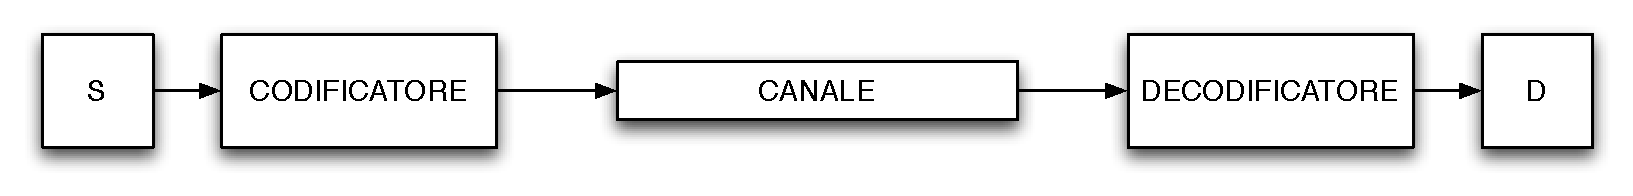
\includegraphics[width=\textwidth]{img/intro2.pdf}
\caption{sistema di comunicazione dotato di codificatore e decodificatore}
\label{fig:0006}
\end{center}
\end{figure}

Ponendosi in un caso ancora più generale, è necessario considerare anche la presenza del rumore. Tipicamente infatti non è possibile 
avere un canale di comunicazione \emph{affidabile}. A causa di molti fattori (e.g. interferenze) sarà infatti possibile che ciò che 
viene inviato dalla sorgente non coincida con quanto ricevuto dal destinatario. Quest'ultimo scenario è rappresentato in figura 
\ref{fig:0007}.

\begin{figure}[htbp]
\begin{center}
	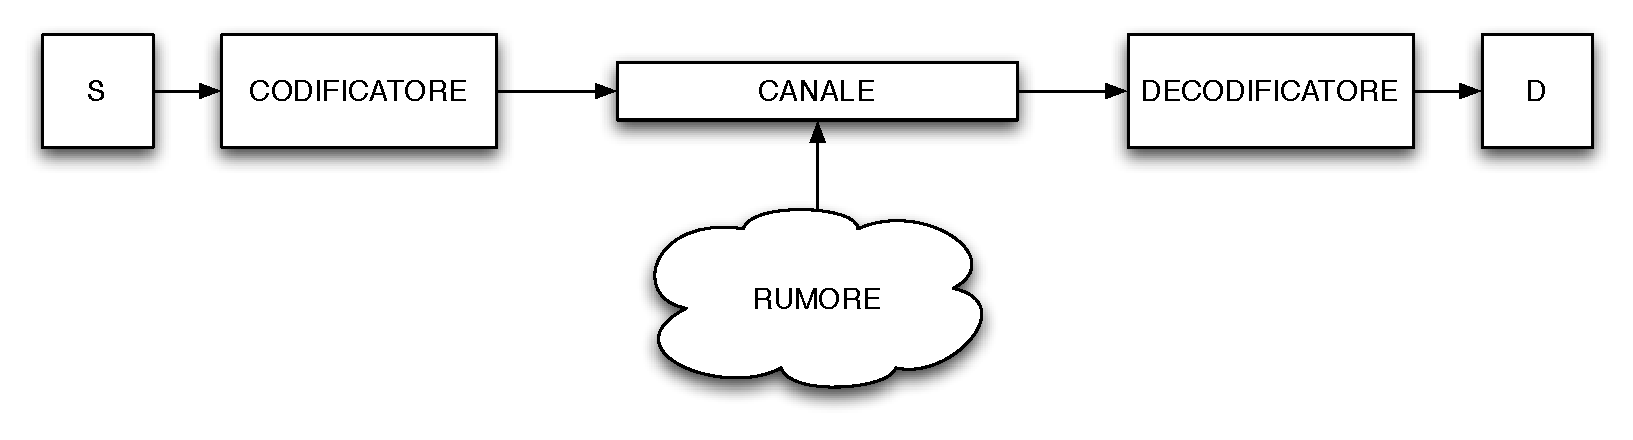
\includegraphics[width=\textwidth]{img/intro3.pdf}
\caption{sistema di comunicazione dotato di codificatore e decodificatore, con presenza di rumore}
\label{fig:0007}
\end{center}
\end{figure}

La teoria dell'informazione si occupa dunque di problemi che coinvolgono la trasmissione di informazione da un luogo a un altro, o da un tempo ad un altro (ad esempio la memorizzazione di file in un hard disk per una successiva lettura). In questo ultimo caso 
sorgente e destinazione coincidono.
I problemi di base da affrontare sono due:
\begin{enumerate}
\item \textbf{efficienza}: Migliorare l'efficienza della trasmissione, riducendo la quantità di informazione inviata.
In questo modo è possibile aumentare la velocità di trasmissione (o ridurre le dimensioni da memorizzare nell'esempio dell'hard disk).
\item \textbf{affidabilità}: Rendere la comunicazione affidabile nel caso del rumore, introducendo quindi dell'informazione aggiuntiva 
che consenta di ricostruire l'informazione originale, anche in presenza di errori.
\end{enumerate}

I due problemi sono collegati da un concetto chiave, che è quello di \textbf{ridondanza}. In generale infatti per aumentare l'efficienza si cercherà di eliminare l'informazione ``inutile'', riducendo il messaggio al minimo necessario per renderlo comprensibile. Per aumentare invece l'affidabilità sarà necessario aggiungere informazione, in maniera da poter individuare e correggere eventuali errori 
in fase di trasmissione.
Si tratta dunque di due problemi chiaramente in contrasto.

\noindent
Alcune osservazioni:
\begin{enumerate}
\item il canale considerato è unidirezionale: nei contesti reali i canali sono invece spesso bidirezionali. Possiamo però pensare semplicemente a due canali differenti con uno scambio di ruoli tra l'entità sorgente e l'entità destinatario
\item la sorgente e il destinatario sono unici, mentre nella realtà possono esserci n sorgenti e m destinatari, collegati con k canali, con flussi bidirezionali (pensiamo ai sistemi multimediali); questo fa parte dell'area della teoria dell'informazione che si occupa del broadcasting (diffusione delle informazioni) che non saranno considerate.
\end{enumerate}


Facciamo ora un esempio concreto: in figura \ref{fig:bsc} è rappresentato un \textbf{Binary Symmetric Channel (BSC)}.
\begin{figure}[htbp]
\begin{center}
	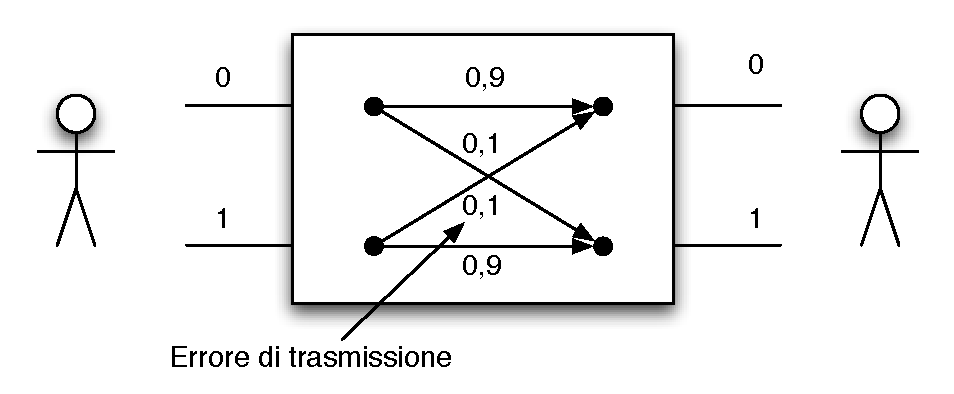
\includegraphics[width=0.7\textwidth]{img/bsc.pdf}
\caption{Binary Symmetric Channel}
\label{fig:bsc}
\end{center}
\end{figure}
Si tratta di un canale caratterizzato da due ingressi e due uscite. Supponiamo di conoscere statisticamente il canale e di aver 
compreso, dopo averlo osservato, che quando la sorgente invia 0, il destinatario riceve 0 il 90\% delle volte, mentre riceve 1 nel 10\% dei casi (c'è quindi una probabilità di errore). La stessa cosa è stata osservata anche per quel che riguarda la trasmissione di 1.
Per migliorare l'affidabilità del canale, possiamo inviare delle terne di bit. Per esempio, quando la sorgente vuole 
inviare 0 viene in realtà mandato 000, mentre quando vuole mandare 1 viene inviato 111. Il destinatario considererà come simbolo 
inviato, quello che appare più volte nel messaggio che riceve (e.g. 0 se riceve 001, 1 se riceve 111).
Con questa semplice tecnica abbiamo aumentato l'affidabilità del canale (chiaramente la probabilità di errore è più bassa), tuttavia 
ciò è avvenuto a scapito dell'efficienza. Dobbiamo infatti inviare il triplo dei simboli necessari, riducendo quindi di un fattore 3 
la velocità di trasmissione.

Sebbene sembri difficile conciliare queste due esigenze, un compromesso è rappresentato dal \textbf{secondo teorema di Shannon}, presentato alla fine della dispensa. Si tratta di un teorema non costruttivo: Shannon non fornisce il codice in questione, ma fornisce una dimostrazione sull'assurdità della non esistenza di tale codice, che ad oggi comunque non è stato ancora trovato (ci si è però avvicinati molto con i turbo-code).

\noindent
Definiamo ora in maniera più formale alcuni concetti.

\begin{definizione}[sorgente]
Si dice \textit{sorgente} un insieme di simboli \(\{s_1, s_2 ... s_n\}\).
\end{definizione}

\noindent
Conosciamo la sorgente quando conosciamo la probabilità con cui viene emesso ciascun simbolo.

\noindent
Possiamo distinguere tra:
\begin{enumerate}
\item \textbf{sorgenti discrete}: se possono generare un numero finito di simboli (quelle che prenderemo in esame)
\item \textbf{sorgenti continue}: se possono generare un numero infinito di simboli
\end{enumerate}

\noindent
Un'ulteriore distinzione è fra:
\begin{enumerate}
\item \textbf{sorgenti a memoria zero}: in cui l'emissione dei simboli è indipendente dai simboli generati in precedenza
\item \textbf{sorgenti con memoria}: quelle che troviamo tipicamente nel mondo reale, caratterizzate da una certa dipendenza della generazione dei simboli rispetto ai precedenti
\end{enumerate}

Nel nostro caso il concetto di sorgente coincide con il concetto di variabile aleatoria. C'è infatti una una corrispondenza perfetta tra i due: la sorgente emette simboli casuali caratterizzati ognuno da una probabilità di essere generato.

Supponiamo quindi che X sia una variabile aleatoria il cui dominio è \(\X = \{x_1, x_2 ... x_n\}\) caratterizzata da una distribuzione di probabilità \(p(x) = Pr\{X = x\}\), con \(x \in \X\).

Il problema che ci poniamo è quello di stabilire quanto sia informativa la sorgente: per far questo dobbiamo innanzitutto stabilire cosa si intende per informazione. L'informazione può essere considerata a 3 diversi livelli di crescente complessità:
\begin{enumerate}
\item \textbf{simbolico} (o sintattico): riguarda i singoli simboli e il modo in cui interagiscono tra loro, i vincoli di varia natura, non si preoccupa del significato;
\item \textbf{semantico}: riguarda ciò che la sorgente vuol dire al destinatario a livello di significato, si tratta di un'astrazione del modello della frase;
\item \textbf{pragmatico}: si distingue dalla semantica per ciò che la sorgente vuole intendere (ad esempio, se considero il messaggio ``Sai che ora è?'', non voglio una risposta sì/no, ma l'ora, ed è qui che entra in gioco la pragmatica, che riguarda ciò che voglio dire).
\end{enumerate}

\noindent
La teoria dell'informazione di Shannon si occupa dell'informazione a livello simbolico.

\medskip
\noindent
La dispensa è articolata in tre parti:
\begin{enumerate}
\item \textbf{formalizzazione della teoria dell'informazione}: in cui saranno date le definizioni di entropia e gli altri concetti chiave della teoria dell'informazione
\item \textbf{problemi di trasmissione in assenza di rumore}: dove ci si concentrerà sull'efficienza (ignorando il rumore), cercando quindi di eliminare la ridondanza
\item \textbf{problemi di trasmissione in presenza di rumore}: in cui si concentrerà sulla realizzazione di una trasmissione affidabile, cercando di conciliare efficienza e affidabilità
\end{enumerate}
\chapter{Entropia}

\section{Definizione di entropia}

\begin{definizione}[entropia]
Si dice \textit{entropia} il contenuto informativo medio di una sorgente S.
\end{definizione}

Dato un generico evento E come possiamo materialmente definire il contenuto informativo I(E) di questo evento? Shannon parte dalla considerazione che l'osservatore ha un patrimonio di conoscenze acquisite e di conseguenza ha una certa idea della probabilità che tale evento si verifichi. L'idea di base è che il contenuto informativo ha a che fare con l'incertezza: più l'osservatore è sorpreso nel 
vedere un simbolo, più il livello di contenuto informativo sarà alto (e viceversa).
Quindi più la probabilità di un evento è bassa, più sarà alto il suo I(E) se tale evento si verifica, fino ad arrivare all'estremo di un evento con probabilità prossima a 0, che avrà un contenuto informativo tendente a infinito.

Possiamo quindi dire che il contenuto informativo di un evento sarà funzione della sua probabilità:
\[I(E) = f(P(E))\]
Proviamo ora a enumerare quali proprietà debba avere la funzione f affinchè il ragionamento fatto finora abbia senso:
\begin{enumerate}
\item f dovrebbe essere definita nell'intervallo \((0,1]\) (aperto a sinistra). Infatti l'argomento di f è una probabilità (che per 
definizione è compresa tra 0 e 1). Inoltre escludiamo lo 0, in quanto in tal caso l'evento non si verifica mai e non è quindi di interesse. Si deve quindi avere:
\[f: (0,1] \longrightarrow \R^+\]
\item f(1) = 0, in quanto l'evento certo non porta nessuna informazione
\item $\lim_{P(E) \rightarrow 0} f(P(E)) = + \infty$
      In quanto quando la probabilità tende a 0, abbiamo il massimo contenuto informativo (c'è la massima ``sorpresa'').
\item f sarà una funzione continua, in quanto non ci aspettiamo che ci siano dei ``salti'' di probabilità
\item f sarà una funzione monotona decrescente (strettamente)
\item consideriamo 2 eventi indipendenti \(E_1\) ed \(E_2\) (esempio: ``oggi c'è il sole'' ed ``è uscita testa dal lancio di una moneta'') , il contenuto informativo dell'intersezione dei due eventi \(I(E_1 \cap E_2)\) (l'evento congiunto) è dato dalla somma dei rispettivi contenuti informativi:
\[I(E_1 \cap E_2) = I(E_1) + I(E_2)\]
Esprimendo il contenuto informativo utilizzando la funzione f, e tenendo conto che la probabilità dell'evento congiunto è pari al prodotto della probabilità dei singoli eventi otteniamo:
\[
\begin{split}
I(E_1 \cap E_2) &= f(P(E_1 \cap E_2)) \\
&= f(P(E_1) \cdot P(E_2)) 
\end{split}
\]
quindi dovrà essere:
\[I(E_1) + I(E_2) = f(P(E_1) \cdot P(E_2))  \]
ossia (sintesi finale della proprietà):
\[ f(P(E_1) \cdot P(E_2)) = f(P(E_1)) + f(P(E_2)) \]
\end{enumerate}

Una funzione che permette di rispettare la proprietà 6 è il logaritmo (\ref{fig:0010}), in quanto il logaritmo del prodotto di due termini è pari alla somma dei logaritmi dei singoli termini, ma tale funzione non rispetta la proprietà 3. Possiamo però prendere la funzione \(- \log x\) (figura \ref{fig:0011}): questa rispetta tutte le proprietà, per cui Shannon ha definito il \textbf{contenuto informativo di un evento} come \(- \log P(E)\), oppure come \(\log \frac{1}{P(E)}\) (semplice proprietà dei logaritmi).
Shannon dimostra anche che questa funzione è l'unica in grado di rispettare tutte le proprietà.

\begin{figure}[htbp]
\begin{center}
	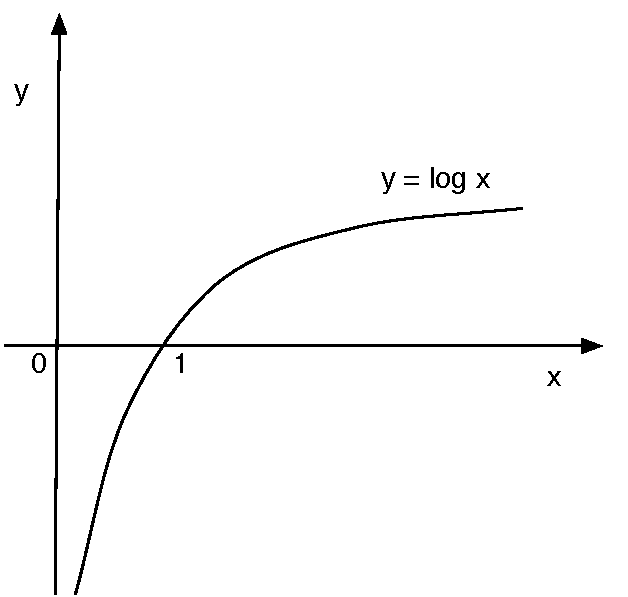
\includegraphics[width=0.6\textwidth]{img/logx.pdf}
\caption{funzione logaritmo}
\label{fig:0010}
\end{center}
\end{figure}

\begin{figure}[htbp]
\begin{center}
	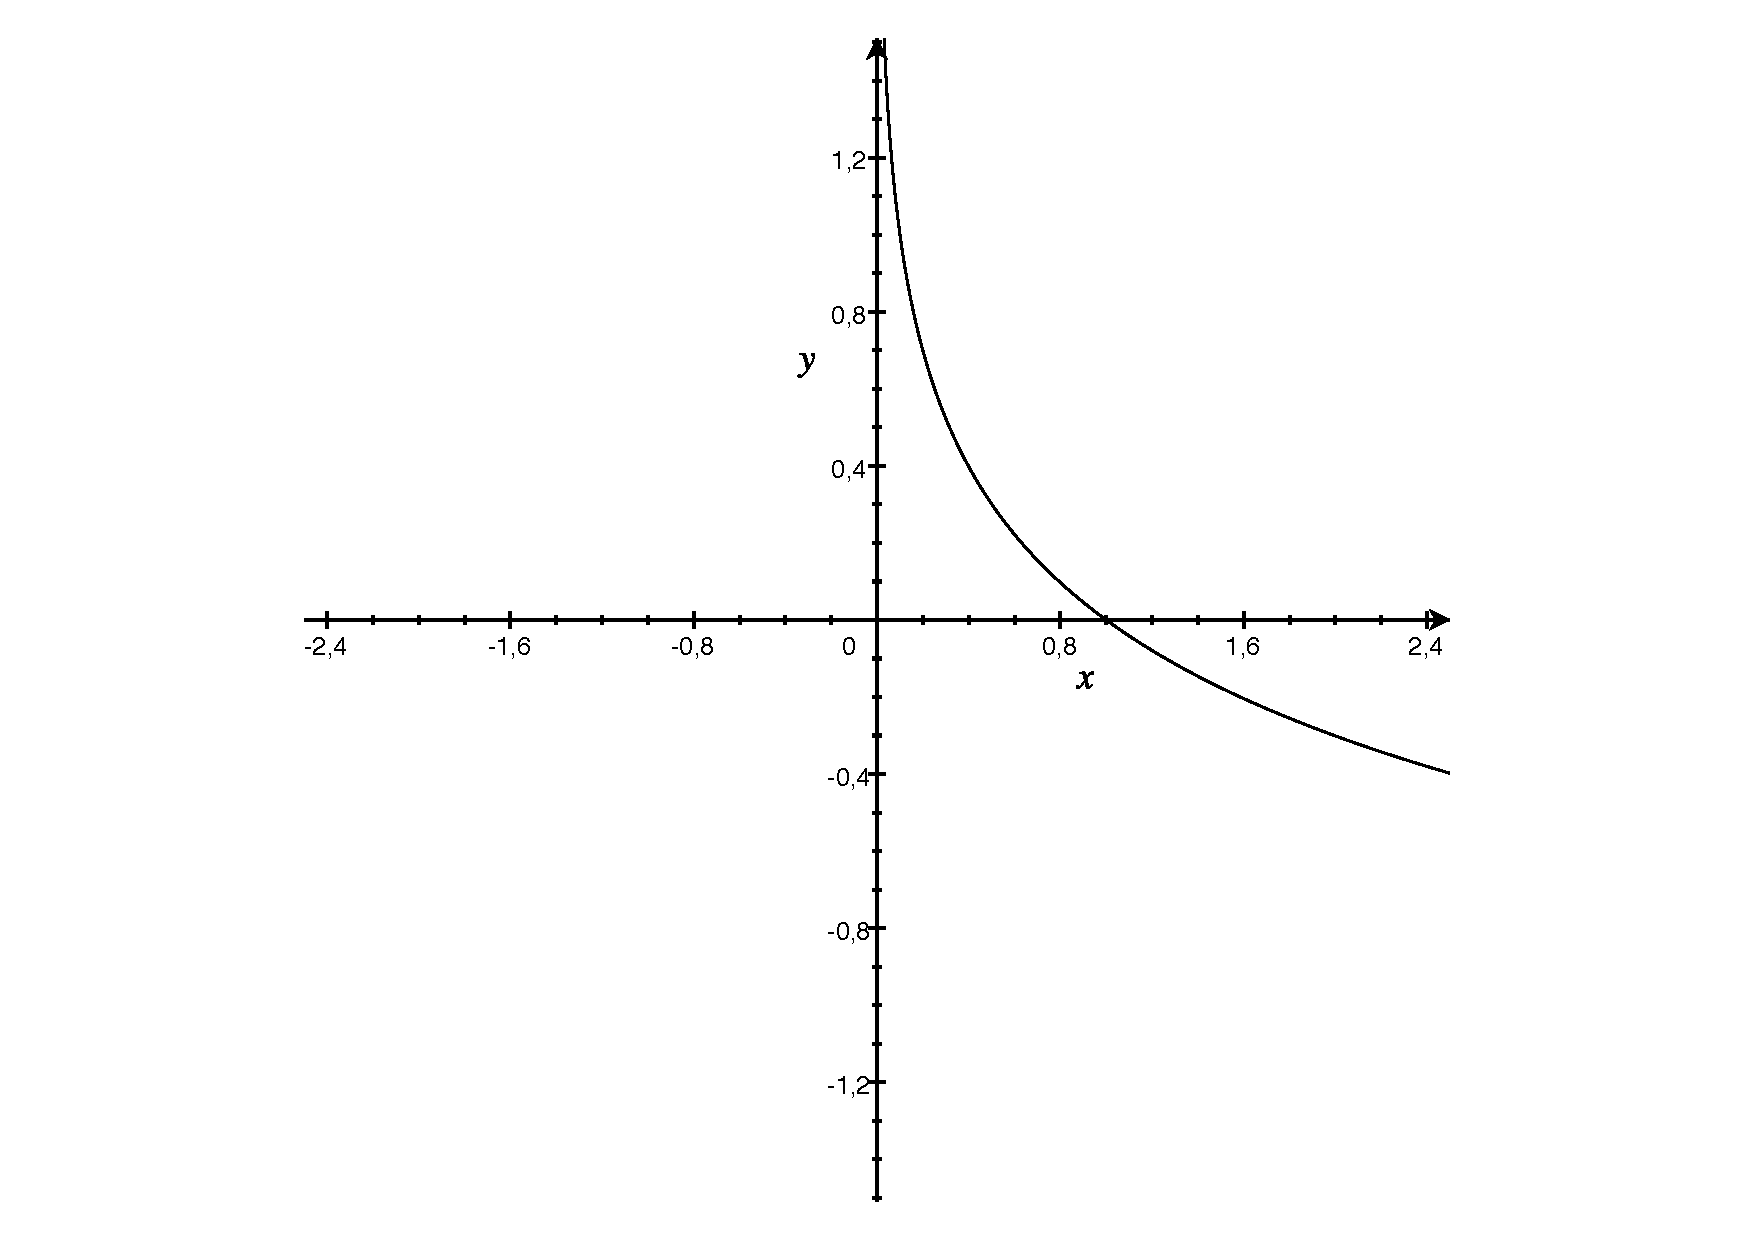
\includegraphics[width=0.6\textwidth]{img/logx2.pdf}
\caption{funzione \(- \log(x)\)}
\label{fig:0011}
\end{center}
\end{figure}

Abbiamo così definito il contenuto informativo di un singolo evento, dobbiamo invece cercare di esprimere il \textbf{contenuto informativo medio} della sorgente. Supponiamo quindi di avere una sorgente che genera una sequenza di simboli \(s_1, s_2, s_3 ... s_n\). Ciascun evento (ovvero simbolo generato) ha contenuto informativo pari a \(I(s_1), I(s_2) ... I(s_n) = -\log p(s_1), -\log p(s_2) ... -\log p(s_n)\). Il contenuto informativo medio della sorgente sarà quindi la media dei contenuti informativi dei singoli eventi:
\[
\begin{split}
H(S) &= \sum_{s \in S} p(s) I(s)\\
&= - \sum_{s \in S} p(s) \log p(s)\\
&= \sum_{s \in S} p(s) \log \frac{1}{p(s)}
\end{split}
\]

In maniera del tutto equivalente, possiamo descrivere la sorgente con una variabile aleatoria (v.a.).
In particolare possiamo considerare la v.a. X, tale che \(\X = \{x_1, x_2 ... x_n\}\).
La probabilità che si verifichi l'evento x è:
\[P\{X = x\} = p(x) \ x \in \X\]
allora il contenuto informativo per tale evento è:
\[I\{X = x\} = - \log p(x)\]
In maniera analoga a prima, il contenuto informativo medio sarà dato dal valore atteso della variabile X.
Questa quantità è proprio l'entropia H(X) (si noti che questo concetto non ha nulla a che fare con quello di entropia della fisica).

\noindent
Formalmente:
\begin{definizione}
\[H(X) \triangleq - \sum_{x \in \X} p(x) \log p(x) = \sum_{x \in \X} p(x) \log \frac{1}{p(x)}\]
\end{definizione}

A questo punto dobbiamo definire l'unità di misura che utilizzeremo. Infatti, al variare della base del logaritmo, cambia 
il valore numerico dell'entropia. In tabella \ref{tab:0001} sono riportate le principali basi utilizzate, con la relativa unità di misura.

\begin{table}[htbp]
	\begin{center}
	\begin{tabular}{ccc}
		\toprule
		Base & Unità di misura \\ 
		\midrule 
		2    & bit             \\ 
		e    & nat             \\ 
		10   & Hartley         \\ 
		\bottomrule               
	\end{tabular}
	\caption{unità di misura utilizzate e basi corrispondenti}
	\label{tab:0001}
	\end{center}
\end{table}

\noindent
Possiamo convertire da una misura all'altra utilizzando la formule dei logaritmi per il cambio di base:
\[\log_b x = \frac{\log_a x}{\log_a b}\]

\noindent
Se si vuole indicare una entropia in una specifica base, si può utilizzare la seguente definizione:
\begin{definizione}[entropia con base a]
Definiamo l' \textit{entropia con base a} come:
\[H_a(X) = - \sum_{x \in \X} p(x) \log_a p(x)\]
\end{definizione}

E' a questo punto necessaria una precisazione riguardante la definizione di entropia che è stata data.
Se supponiamo infatti di avere uno o più simboli dell'alfabeto che non verranno mai generati, si 
hanno degli x per i quali \(p(x) = 0\).
Succede dunque che nel calcolo dell'entropia ci si trova di fronte al calcolo di \(\log 0\), che non è definito.

\noindent
Possiamo però calcolare il limite della quantità in questione:
\[\lim_{p(x) \rightarrow 0} p(x) \log(p(x))\]
\[=\lim_{x \rightarrow 0} \frac{\log p(x)}{\frac{1}{p(x)}}\]
applicando la regola di de l'Hôpital:
\[\lim_{p(x) \rightarrow 0} \frac{\frac{1}{p(x)}}{-\frac{1}{p(x)^2}} = \lim_{p(x) \rightarrow 0} p(x) = 0\]

Per ovviare quindi al precedente problema poniamo \(0 \log 0 = 0\).
Questo ci consente di non considerare le probabilità nulle, in quanto non hanno alcuna influenza sul valore 
dell'entropia.







\section{Studio della funzione entropia}
Risulta utile studiare la funzione entropia (lo faremo in un caso particolare), in maniera tale da avere una idea precisa del suo comportamento.
Innanzitutto però facciamo due osservazioni:
\begin{enumerate}
\item l'entropia è sempre maggiore o uguale a 0:
\[H(x) \geq 0\]
questo perché:
\[H(x) = - \sum_{x \in \X} p(x) \log p(x)\]
ma sappiamo che \(p(x) \geq 0\) e che \(\log p(x) \leq 0\), quindi nel complesso \(p(x) \log p(x)\) sarà sempre negativo, essendoci il segno meno all'esterno della sommatoria, risulta che l'entropia è sempre maggiore o uguale a 0.

\item possiamo cambiare la base dell'entropia (dalla base a alla base b) tramite la seguente formula:
\[H_b(X) = \log_b a \cdot H_a(X) = \frac{H_a(X)}{\log_a b}\]
La dimostrazione è banale, utilizzando la proprietà del cambio di base dei logaritmi.
\end{enumerate}

Prendiamo ora l'esempio di una variabile aleatoria X associata al lancio di una moneta bilanciata, che assume quindi solo i valori 0 (testa) e 1(croce):
\[\X = \{0,1\}\]
\[P\{X = 0\} = 1/2\]
\[P\{X = 1\} = 1/2\]
Si tratta del caso peggiore in quanto non possiamo fare previsioni sul prossimo simbolo emesso, poiché entrambi hanno la stessa probabilità. Vediamo quanto vale l'entropia in questo caso:
\[
\begin{split} 
H(X) &= - P(X = 0) \cdot \log P(X = 0) - P(X = 1) \cdot \log P(X = 1)\\ 
&= -\frac{1}{2} \log{\frac{1}{2}} -\frac{1}{2} \log{\frac{1}{2}}\\ 
&= - \frac{1}{2} \log{2^{-1}} - \frac{1}{2} \log{2^{-1}}\\
&= - \frac{1}{2} (-1) \log{2} - \frac{1}{2} (-1) \log{2}\\
&= \frac{1}{2} \log{2} + \frac{1}{2} \log{2} = 1 bit
\end{split} 
\]
Abbiamo quindi anallizzato solo il caso particolare in cui la moneta è bilanciata, ovvero il caso in cui le probabilità di generazione dei vari simboli siano tutte uguali. Proviamo ora a generalizzare la nostra analisi prendendo in esame la famiglia di sorgenti binarie, introducento un parametro p. Tale parametro esprimere la probabilità di generazione dei 2 simboli (al variare di p ottengo sorgenti diverse):
\[X \ v.a. \qquad \X = \{0,1\}\]
\begin{align*}
p(0) &= P(X = 0) = p \quad 0 \leq p \leq 1 \\
p(1) &= P(X = 1) = 1-p
\end{align*}
Calcolando l'entropia generalizzata:
\[H(p) = - p \log{p} -(1-p) \log (1-p) \mbox{ con } p \in [0,1]\]

\noindent
Studiamo ora il comportamento di questa funzione (figura \ref{fig:entropia}).

\noindent
Osserviamo che:
\begin{enumerate}
\item qualsiasi entropia è sempre maggiore o uguale a 0
\item negli estremi dell'intervallo la funzione assume valori (ricordando che abbiamo posto \(0 \log 0 = 0\)):
\[H(0) = - 0 \log{0} -(1-0) \log (1-0) = 0\] 
\[H(1) = - 1 \log{1} -(1-1) \log (1-1) = 0\]
dall'esempio precedente sappiamo inoltre che \(H(1/2) = 1\);
\item si può notare una certa simmetria, tale che \(H(p) = H(1-p)\) infatti:
\[
\begin{split}
H(1-p) &= - (1- p) \log{(1-p)} -(1- 1 + p) \log (1- 1 + p) \\
&= - (1- p) \log{(1-p)} - p \log p = H(p)
\end{split}
\]
\item studiando la derivata possiamo capire quali siano i punti di minimo e massimo:
\[
\begin{split} 
D \ H(p) &= \frac{d H(p)}{d p} \\ 
&= - \frac{d [p \log p + (1-p) \log (1-p)]}{d p} \\ 
&= - [\log p + \cancel{p} \frac{1}{\cancel{p}} \log e - \log{(1-p)} - \cancel{(1-p)} \frac{1}{\cancel{(1-p)}}\log e] \\ 
&= - [\log p +  \cancel{\log e} - \log{(1-p)} - \cancel{\log e}] \\ 
&= \log (1-p) - \log p \\ 
\end{split} 
\]
per trovare i punti di massimo è sufficiente controllare quando si annulla la derivata:
\[\frac{d H(p)}{d p} = 0 \Longrightarrow \log (1-p) \cdot \log p = 0 \iff 1-p = p \iff p = 1/2\]
Quindi c'è un unico punto in cui si annulla, ossia il massimo valore assunto dall'entropia è:
\[H(1/2) = 1\]
\item H(p) è concava\footnote{
\begin{definizione}[funzione convessa]
Data la funzione:
\[f: [a,b] \longrightarrow \R \]
f si dice \textit{funzione convessa} se
\[\forall x_1, x_2 \in [a,b], \lambda \in [0,1] \quad f(\lambda x_1 + (1-\lambda)x_2) \leq \lambda f(x_1) + (1-\lambda) f(x_2)\]
\end{definizione}

\begin{definizione}[funzione concava]
Data la funzione:
\[f: [a,b] \longrightarrow \R \]f si dice \textit{funzione concava} se -f è convessa.
\end{definizione}
} per il teorema descritto nella nota a piè di pagina\footnote{
\begin{teorema}
se \(f \in \E^1\) (ossia se f è derivabile almeno 1 volta) allora:
\[\mbox{f convessa} \iff \forall x, x_0 \in [a,b] : f(x) \geq f(x_0) + f'(x_0) (x-x_0)\]
\label{concava1}
\end{teorema}

\begin{teorema}
se \(f \in \E^2\) (ossia se f è derivabile almeno 2 volte) allora:
\[\mbox{f convessa} \iff \forall x \in [a,b]: f''(x) \geq 0\]
\label{concava}
\end{teorema}
}, infatti:
\[
\begin{split} 
H''(p) &= \frac{d^2 H(p)}{dp^2} = \\ 
&= \frac{d [\log(1-p) - \log p]}{dp} \\ 
&= - \frac{1}{1-p}\log e - \frac{1}{p} \log e < 0 \ \forall \ p \in [0,1]
\end{split} 
\]
in quanto per \(p \in [0,1]\) sia \(- \frac{1}{1-p}\) sia \(- \frac{1}{p}\) sono negativi;
\item la funzione è simmetrica rispetto all'asse verticale \(p = \frac{1}{2}\); per dimostrarlo deve essere che \(\forall \ q \leq 1/2\):
\[H(1/2 - q) = H(1/2 + q)\]
ma sappiamo che:
\[H(p) = H(1-p)\]
quindi:
\[H(1/2 + q) = H(1-(1/2 - q)) = H(1/2 - q)\]
pertanto la funzione entropia ha una forma a campana simmetrica (figura \ref{fig:entropia}).
\end{enumerate}
Si ricordi che questo studio è stato effettuato nel caso di 2 variabili (i grafici sono infatti bidimensionali). E' possibile (sebbene 
sia abbastanza complicato), estendere quanto visto al caso generale con n variabili.

\begin{figure}[htbp]
\begin{center}
	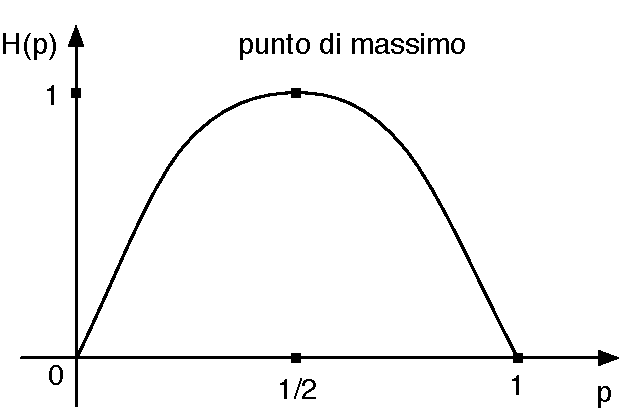
\includegraphics[width=0.6\textwidth]{img/entropia.pdf}
\caption{studio della funzione H(p)}
\label{fig:entropia}
\end{center}
\end{figure}










\section{Proposizioni sull'entropia}
Vengono ora presentate alcune proposizioni che hanno come oggetto l'entropia.
Tuttavia, per dimostrare formalmente la loro validità, sarà necessario introdurre prima 
alcuni concetti e risultati.
\subsection{Simplesso standard}

\begin{figure}[htbp]
  \centering
  \subfloat[n=2]{\label{fig:simpl2}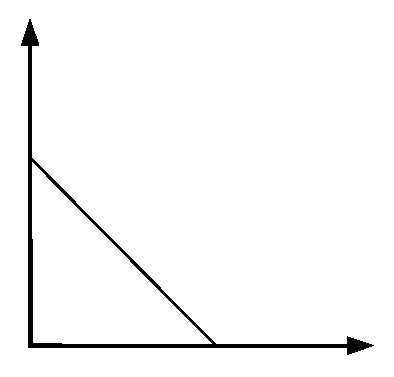
\includegraphics[width=0.4\textwidth]{img/simplex2.pdf}}                
  \subfloat[n=3]{\label{fig:simpl3}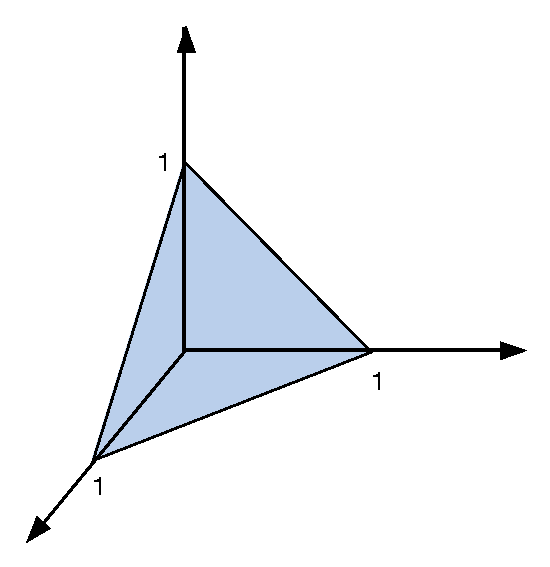
\includegraphics[width=0.4\textwidth]{img/simplex3.pdf}}
  \caption{Rappresentazione del simplesso standard}
  \label{fig:animals}
\end{figure}

Il simplesso standard di $R^n$ o spazio delle probabilità n-dimensionale, è definito come segue:
\begin{definizione}[Simplesso standard]

 \[ \triangle_n = \{ \bar{x} \in R^n \mid \sum_{i=1}^{n} x_i=1 \ ; \ \forall i=1..n: x_i \ge 0 \} \]
\end{definizione}

Per chiarire meglio il concetto, facciamo due esempi:
\begin{itemize}
 \item Nel caso in cui n=2, abbiamo il simplesso standard unidimensionale (figura \ref{fig:simpl2}).
       Deve essere che $x_1 \ge 0, x_2 \ge 0$ e che $x_1+x_2=1$. Nella figura $x_1$ è rappresentato 
       sull'asse x, mentre $x_2$ sull'asse y (l'inverso è equivalente).
       Si ottiene dunque un segmento.
 \item Nel caso in cui n=3, abbiamo il simplesso standard bidimensionale (figura \ref{fig:simpl3}).
       In questo caso si ottiene un triangolo.
\end{itemize}





\subsection{Disuguaglianza di Gibbs}
Prima di introdurre la disuguaglianza di Gibbs, presentiamo un lemma che sarà utile 
per dimostrare la validità della disuguaglianza.

\begin{lemma}

 \[ln(x) \le x-1 \] 
 \begin{proof}
  Sia $y=ln(x)$, allora $y'=\frac{1}{x}$ e $y''=-\frac{1}{x^2}$.

  Poiché $y''$ è sempre negativa, la funzione y è strettamente concava (Teorema \ref{concava}).
  Ma se una funzione è concava, per il teorema \ref{concava1} deve essere:
  \[ f(x) \le f(x_0) + f'(x_0)(x-x_0) \]
  
  Quindi per la funzione y:
  \[ ln(x) \le ln(x_0) + \frac{1}{x_0}(x-x_0) \]

  Ponendo $x_0=1$ risulta:
  \[ ln(x) \le x-1 \]
 \end{proof}
  \label{lemma_entr}
\end{lemma}

\begin{osservazione}
 Il lemma precedente può essere esteso anche al caso di un logaritmo con base qualunque.
 In particolare risulta:
 \[log(x) \le log(e)(x-1) \]
 La dimostrazione è banale e si basa sulla formula per il cambio di base tra logaritmi.
\end{osservazione}


\begin{lemma}[disuguaglianza di Gibbs o lemma del logaritmo]

 \[Dati \ \bar{p} \ e \  \bar{q} \in \triangle_n:\] 
 \[ -\sum_{i=1}^n p_i log(p_i) \le - \sum_{i=1}^n p_i log(q_i) \]

 \begin{proof}
    
   Supponiamo che $\forall i=1..n$: $p_i>0 \ e \ q_i>0$.
  Se così non fosse possiamo avere i seguenti casi:

  \begin{itemize}
   \item $p_i=0 \ e \ q_i=0$: si ha che l'elemento delle sommatorie è 0log(0), che per la convenzione 
   stabilita in precedenza, vale 0. In questo caso quindi possiamo ignorare gli elementi
   in quanto non modificano il valore delle sommatorie.
   \item $p_i=0 \ e \ q_i \ge 0$: in questo caso si ha 0log(0) nella parte sinistra (risulta 0
   come nel caso di prima). Nella parte destra invece $0log(q_i)$ è banalmente 0.
   Il caso è quindi analogo al precedente.
   \item $p_i \ge 0 \ e \ q_i=0$: in questo caso la disuguaglianza è vera. 
   Infatti si avrebbe $p_i log(0)$. Ma passando al limite log(0) tende a $- \infty$. 
   La parte destra della disuguaglianza è dunque $+ \infty$.
  \end{itemize}

   Poiché $p_i>0 \ e \ q_i>0$:
   \[ \frac{q_i}{p_i}>0 \].
   Per il lemma \ref{lemma_entr} si ha:
   \[ ln \left( \frac{q_i}{p_i} \right) \le \frac{q_i}{p_i} - 1 \]
   \[ \Rightarrow p_i ln \left( \frac{q_i}{p_i} \right) \le p_i \left [ \frac{q_i}{p_i} - 1 \right ] \]
   \[ \Rightarrow \sum_{i=1}^{n} p_i ln \left( \frac{q_i}{p_i} \right) \le 
      \sum_{i=1}^{n} p_i \left [ \frac{q_i}{p_i} - 1 \right ] 
       = \sum_{i=1}^{n} q_i - \sum_{i=1}^n p_i = 1-1 = 0
   \]
   \[ \Rightarrow \sum_{i=1}^{n} p_i ln \left( \frac{q_i}{p_i} \right) \le 0 \]
   \[ \Rightarrow \sum_{i=1}^{n} p_i ln \left( \frac{1}{p_i} \right) +
    \sum_{i=1}^{n} p_i ln \left( q_i \right) \le 0 \]
   \[ \Rightarrow \sum_{i=1}^{n} p_i ln \left( \frac{1}{p_i} \right) \le
    -\sum_{i=1}^{n} p_i ln \left( q_i \right) \]
  \[ \Rightarrow -\sum_{i=1}^{n} p_i ln \left( p_i \right) \le
    -\sum_{i=1}^{n} p_i ln \left( q_i \right) \]

  Il lemma è stato dimostrato per il logaritmo naturale, tuttavia tramite la solita proprietà per il cambio di base
  risulta chiaro che la diseguaglianza vale con qualunque base.
 \end{proof}
 \label{gibbs}
\end{lemma}

\begin{osservazione}
 \[ -\sum_{i=1}^n p_i log(p_i) = - \sum_{i=1}^n p_i log(q_i) \iff \bar{p}=\bar{q}\]
\end{osservazione}







\subsection{Proposizioni}
Introdotti i concetti nei due paragrafi precedenti, possiamo ora enunciare e dimostrare 
le proposizioni:
\begin{proposizione}
 \[H(\bar{p})=0 \iff \exists i \in \{1..n\} \mid p_i=1  \]

  \begin{proof}
  \[H(\bar{p})=-\sum_{i=1}^{n}p_i log(p_i)=0 \iff \]
  \[ \forall i=1..n \ : \ p_i log(p_i)=0 \iff 
    p_i=0 \ \lor \ p_i=1 \iff \exists i \mid p_i=1 \]
  \end{proof}
\end{proposizione}

\begin{proposizione}
\label{propen}
 \[H(\bar{p}) \le H(\frac{1}{n},\frac{1}{n},...,\frac{1}{n})=log(n)  \]

  \begin{proof}
  Per la diseguaglianza di Gibbs (\ref{gibbs}):
  \[ H(\bar{p})=-\sum_{i=1}^n p_i log(p_i) \le -\sum_{i=1}^n p_i log(q_i)  \]

  \[Poniamo \ \bar{q}=\left ( \frac{1}{n},\frac{1}{n},...,\frac{1}{n} \right) \]

  \[ \Rightarrow -\sum_{i=1}^{n} p_i log(p_i) \le
    -\sum_{i=1}^{n} p_i log \left (\frac{1}{n} \right) \]

  \[ \Rightarrow -\sum_{i=1}^{n} p_i log(p_i) \le
    \sum_{i=1}^{n} p_i log(n) = log(n) \sum_{i=1}^{n} p_i = log(n) \]

  \[Ricordiamo che \sum_{i=1}^{n} p_i = 1 in quanto p_i \in \delta_n (simplesso standard) \forall i = 1, 2, ..., n \]

  \[ \Rightarrow H(\bar{p}) \le log(n) \]
  Resta da dimostrare che \[H(\frac{1}{n},\frac{1}{n},...,\frac{1}{n})=log(n) \]
  Che può essere provato calcolando direttamente l'entropia:

  \[H(\frac{1}{n},\frac{1}{n},...,\frac{1}{n})=\sum_{i=1}^n \frac{1}{n} log(n)=log(n) \sum_{i=1}^n \frac{1}{n}=log(n) \]


  \end{proof}
\end{proposizione}

\begin{proposizione}
 \[0 \le H(\bar{p}) \le log(n) \]

  \begin{proof}
   L'entropia è maggiore o uguale a 0 per definizione ed è 
   minore od uguale a log(n) per la proposizione \ref{propen}.
  \end{proof}
\end{proposizione}










\section{Entropia congiunta e condizionata}
Abbiamo definito l'entropia di una singola variabile casuale. Possiamo estendere questa definizione 
considerando invece due variabili casuali e definendo l'entropia congiunta.

In dettaglio consideriamo le variabili:
\[X=\{x_1..x_n\} \ e \ Y=\{y_1..y_n\}\]
Poniamo inoltre:
\[Pr\{X=x\}=p(x) \ e \ Pr\{Y=y\}=p(y) \]
\[Pr\{X=x,Y=y\}=p(x,y) \ e \ Pr\{X=x/Y=y\}=p(x/y) \]

\begin{definizione}
 L'entropia congiunta H(X,Y) di due variabili casuali X e Y è:
 \[ H(X,Y)=-\sum_{x \in X} \sum_{y \in Y} p(x,y)log( p(x,y) ) \]
\end{definizione}

Possiamo anche definire il concetto di entropia condizionata.
A tal scopo è utile ricordare la definizione di probabilità condizionata:
  \[ p(a/b)=\frac{p(a,b)}{p(b)} \]

Vogliamo in sostanza chiederci quale sia l'entropia della variabile X, supponendo di conoscere la variabile Y.
Possiamo innazitutto calcolare il valore dell'entropia condizionata ad uno specifico evento y.
In questo caso si ha:
\[
 H(X/Y=y)= -\sum_{x \in X} p(x/y)log(p(x/y))
\]

A partire da questo risultato, l'entropia condizionata può essere ottenuta semplicemente 
come valore atteso al variare di tutti gli eventi $y_i \in Y$.

\begin{definizione}
 L'entropia condizionata H(X/Y) di due variabili casuali X e Y è:
 \[
  \begin{split}
    H(X/Y) &=  \sum_{y \in Y}p(y)H(X/Y=y)  \\
         &= -\sum_{y \in Y} p(y) \sum_{x \in X} p(x/y)log(p(x/y) \\
         &= -\sum_{x \in X} \sum_{y \in Y} p(x,y)log( p(x/y) )
  \end{split}
  \]
 (l'ultimo passaggio deriva direttamente dalla definizione di probabilità condizionata)
\end{definizione}

E' lecito domandarsi se esista un legame tra entropia, entropia congiunta ed entropia condizionata.
La risposta è si, come risulta dal seguente teorema.

\begin{teorema}[Regola della catena]
 \[ H(X,Y)=H(X)+H(Y/X)=H(Y)+H(X/Y) \]
 \begin{proof}
  \[
   \begin{split}
    H(X,Y) &=  -\sum_{x \in X} \sum_{y \in Y} p(x,y) log(p(x,y))  \\
         &= -\sum_{x \in X} \sum_{y \in Y} p(x,y) log \left [p(x) p(y/x) \right] \\
         &= -\sum_{x \in X} \sum_{y \in Y} p(x,y)log(p(x)) - \sum_{x \in X} \sum_{y \in Y} p(x,y)log(p(y/x)) \\
         &= -\sum_{x \in X} p(x)log(p(x)) - \sum_{x \in X} \sum_{y \in Y} p(x,y)log(p(y/x)) \\
         &= H(X) + H(Y/X)
  \end{split}
  \]
  In maniera del tutto analoga si dimostra l'altra equivalenza.
 \end{proof}
\label{catena}
\end{teorema}

\begin{corollario}
\[
 H(X,Y/Z)=H(X/Z)+H(Y/X,Z)
\]
\begin{proof}
In maniera analoga a quanto fatto per l'entropia condizionata, calcoliamo inizialmente per un valore fissato 
(in questo caso per un $z \in Z$).
\[
 H(X,Y/Z=z)=-\sum_{x \in X} \sum_{y \in Y} p(x,y/z) log(p(x,y/z))
\]

\noindent
Utilizziamo quindi il valore atteso (sempre analogamente a prima) per calcolare l'entropia:

\[\begin{split}
 H(X,Y/Z)&=\sum_{z \in Z} p(z) H(X,Y/Z=z) \\
 &=-\sum_{z \in Z} p(z) \sum_{x \in X} \sum_{y \in Y} p(x,y/z) log(p(x,y/z)) \\
 &=-\sum_{x \in X} \sum_{y \in Y} \sum_{z \in Z} p(x,y/z) p(z) log(p(x,y/z)) \\ 
 &=-\sum_{x \in X} \sum_{y \in Y} \sum_{z \in Z} p(x,y,z) log(p(x,y/z)) \\
 \end{split}
\]

A questo punto, in maniera analoga al teorema:
\[\begin{split}
 H(X,Y/Z)=&-\sum_{x \in X} \sum_{y \in Y} \sum_{z \in Z} p(x,y,z) log(p(x,y/z)) \\
 =&-\sum_{x \in X} \sum_{y \in Y} \sum_{z \in Z} p(x,y,z) log[p(x/z) p(y/x,z)] \\
 =&-\sum_{x \in X} \sum_{y \in Y} \sum_{z \in Z} p(x,y,z) log(p(x/z)) \\
   &-\sum_{x \in X} \sum_{y \in Y} \sum_{z \in Z} p(x,y,z)log(p(y/x,z) \\
 =&-\sum_{x \in X} \sum_{z \in Z} p(x,z) log(p(x/z)) -\sum_{x \in X} \sum_{y \in Y} \sum_{z \in Z} p(x,y,z)log(p(y/x,z) \\
 =& H(X/Z)+H(Y/X,Z)
 \end{split}
\]
\end{proof}
\end{corollario}


\bigskip 

\noindent
Per provare l'utilità della regola della catena, applichiamola ad un esempio concreto.

\smallskip
\noindent
\textbf{Esempio.}
Consideriamo due v.a. X,Y le cui probabilità congiunte sono riportate in tabella \ref{tab:catena}

\begin{table}[htbp]
  \begin{center}
   \begin{tabular}{c|cccc|c}
	Y/X & 1 & 2 & 3 & 4 & p(y)\\
       \hline
	1 & 1/8 & 1/16 & 1/32 & 1/32 & 1/4 \\ 
	2 & 1/16 & 1/8 & 1/32 & 1/32 & 1/4 \\ 
	3 & 1/16 & 1/16 & 1/16 & 1/16 & 1/4 \\ 
        4 & 1/4 & 0 & 0 & 0 & 1/4 \\ 
        \hline
        p(x) & 1/2 & 1/4 & 1/8 & 1/8 & 1 \\  
    \end{tabular}
     
     \caption{Probabilità delle v.a. X e Y}
    \label{tab:catena}
  \end{center}
\end{table}

\noindent
Supponiamo di voler calcolare H(X), H(Y), H(X,Y), H(X/Y) e H(Y/X).
Per calcolare H(X) utilizziamo la definizione di entropia, mentre per
H(Y) possiamo usare la proposizione \ref{propen}.
\[
 \begin{split}
 H(X) &= H \left( \frac{1}{2},\frac{1}{4},\frac{1}{8},\frac{1}{8} \right) \\
      &= \frac{1}{2} log(2) + \frac{1}{4} log(4) + \frac{1}{8} log(8) + \frac{1}{8} log(8) \\
      &= \frac{1}{2} + \frac{2}{4} + \frac{3}{8} + \frac{3}{8} \\
      &= \frac{7}{4} \ bit
 \end{split}
\]

\[
 \begin{split}
 H(Y) &= H \left( \frac{1}{4},\frac{1}{4},\frac{1}{4},\frac{1}{4} \right) \\
      &= log(4) = 2 \ bit
 \end{split}
\]

A questo punto calcoliamo H(X/Y) tramite la definizione di entropia condizionata, mentre
per ottenere H(X,Y) e H(Y/X) possiamo utilizzare la regola della catena.

\[
 \begin{split}
      &H(X/Y)
      = \sum_{y \in Y} p(y) H(X/Y=y)= \\
      &= \frac{1}{4} H(X/Y=1) + \frac{1}{4} H(X/Y=2) +\frac{1}{4} H(X/Y=3) +\frac{1}{4} H(X/Y=4) \\
      &= \frac{1}{4} \left [ 
        H \left( \frac{1}{2},\frac{1}{4},\frac{1}{8},\frac{1}{8} \right) +
        H \left( \frac{1}{4},\frac{1}{2},\frac{1}{8},\frac{1}{8} \right) +
        H \left( \frac{1}{4},\frac{1}{4},\frac{1}{4},\frac{1}{4} \right) +
        H \left(1,0,0,0 \right) 
       \right ]\\
      &= \frac{1}{4} \left [ \frac{7}{4} + \frac{7}{4} + 2 + 0 \right ] \\
      &= \frac{11}{8} \ bit
 \end{split}
\]

\[
  H(X,Y)=H(Y)+H(X/Y)=2+ \frac{11}{8}=\frac{27}{8} \ bit
\]

\[
 H(Y/X)=H(X,Y)-H(X)= \frac{27}{8}-\frac{7}{4}=\frac{13}{8} \ bit
\]

Grazie alla regola della catena abbiamo quindi evitato di calcolare esplicitamente H(Y/X)
e soprattutto H(X,Y). Nel caso di quest'ultima il calcolo sarebbe stato sicuramente molto oneroso.

\bigskip
\bigskip
\bigskip

E' utile estendere la regola della catena a più variabili.

\begin{teorema}[Regola della catena generalizzata]
 \[ H(X_1,X_2,...,X_n)=\sum_{i=1}^n H(X_i/X_{i-1},X_{i-2},...,X_1) \]

\begin{proof}
 Per induzione, sul numero n di variabili.
\begin{description}
 \item[Caso base, n=2] Bisogna dimostrare che:
 \[
  H(X_1,X_2)=H(X_1)+H(X_2/X_1)
 \]
 Ma questa è esattamente la regola della catena (Teorema \ref{catena}).
 \item[Passo induttivo]
  Supponiamo che l'uguaglianza valga per n e dimostriamo che vale anche per n+1.
  Poniamo poi $Z=X_1,X_2,..X_n$. Risulta:
  \[\begin{split}
   H(X_1,X_2,...,X_{n+1})&=H(Z,X_{n+1}) \\
   &=H(Z)+H(X_{n+1}/Z) \\
   &=H(X_1,X_2,..X_n) + H(X_{n+1}/X_1,X_2,..X_n) \\
   \end{split}
  \]
  Ora per ipotesi induttiva:
  \[
   H(X_1,X_2,..X_n)=\sum_{i=1}^n H(X_i/X_{i-1},X_{i-2},...,X_1)
  \]
   Da cui:
  \[\begin{split}
   &H(X_1,X_2,..X_n) + H(X_{n+1}/X_1,X_2,..X_n) \\
   &=\sum_{i=1}^n H(X_i/X_{i-1},X_{i-2},...,X_1) + H(X_{n+1}/X_n,..,X_2,X_1) \\
   &=\sum_{i=1}^{n+1} H(X_i/X_{i-1},X_{i-2},...,X_1) 
   \end{split}
  \]

\end{description}

\end{proof}
\label{catenag}
\end{teorema}


\section{Entropia relativa e informazione mutua}
Fino ad ora abbiamo preso in considerazione l'entropia relativa ad una sola quantità (anche se tale quantità poteva comprendere più variabili condizionate e/o congiunte). Ora siamo invece interessati a dei risultati che leghino tra loro più variabili.
Prima però è necessario introdurre alcuni concetti, utili per le dimostrazioni.

\begin{definizione}[Insieme convesso]
 Un insieme X si dice convesso se comunque presi due punti $x,y \in X$ il segmento che li congiunge è contenuto interamente in X.
 Formalmente, $X \in R^n$ è convesso se:
 \[
  \forall x,y \in X, \lambda \in [0,1] \ : \ \lambda x + (1-\lambda) y \in X
 \]
\end{definizione}

\noindent
In figura \ref{convessi} sono riportati un insieme convesso ed uno non convesso.

\begin{figure}[htbp]
\centering
\subfloat[Convesso]
   {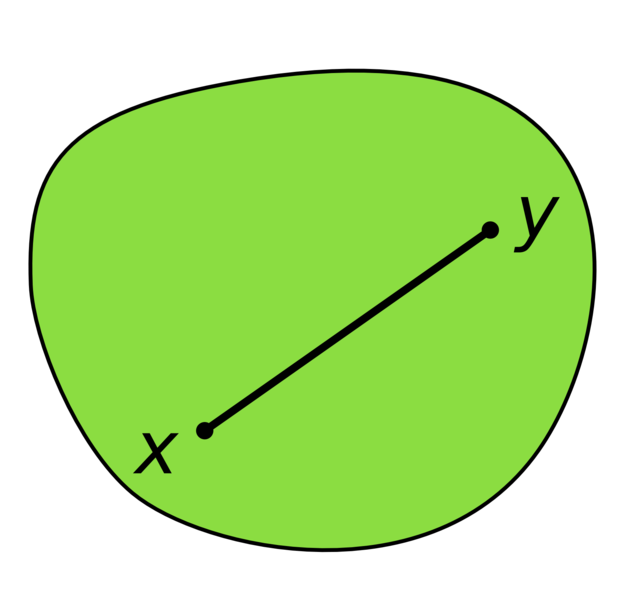
\includegraphics[width=0.30\textwidth]{img/convex2.png}}
\hspace{5mm}
\subfloat[Non convesso]
  {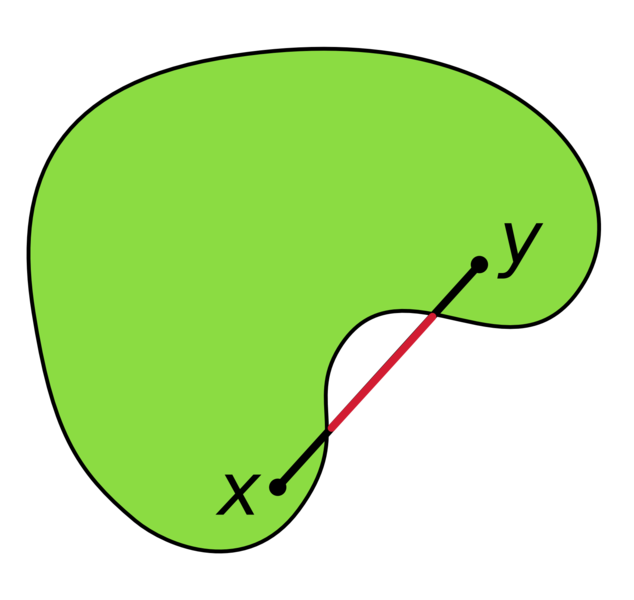
\includegraphics[width=0.30\textwidth]{img/convex1.png}}
\caption{Esempio di insiemi}
\label{convessi}
\end{figure}

\begin{definizione}[Convex Hull]
 Dato un insieme di punti, si dice \textbf{convex hull} (chiusura convessa) il più piccolo insieme convesso che li contiene tutti.
\end{definizione}

Il convex hull si può ottenere congiungendo con dei segmenti, i punti più ``esterni'' dell'insieme. Il convex hull di due punti sarà 
quindi il segmento che li congiunge. In figura \ref{fig:convexhull} è riportato il convex hull di 3 punti $p_1,p_2,p_3$. In generale, con k punti:
\begin{equation}
 CH(p_1,p_2,...,p_k)=\{ p \in R^n \mid p=\sum_{i=1}^k \lambda_i p_i \ \forall \bar{\lambda}=(\lambda_1,\lambda_2,...,\lambda_k) 
\in \Delta_k\}
\label{convex}
\end{equation}

\begin{figure}[htbp]
\begin{center}
	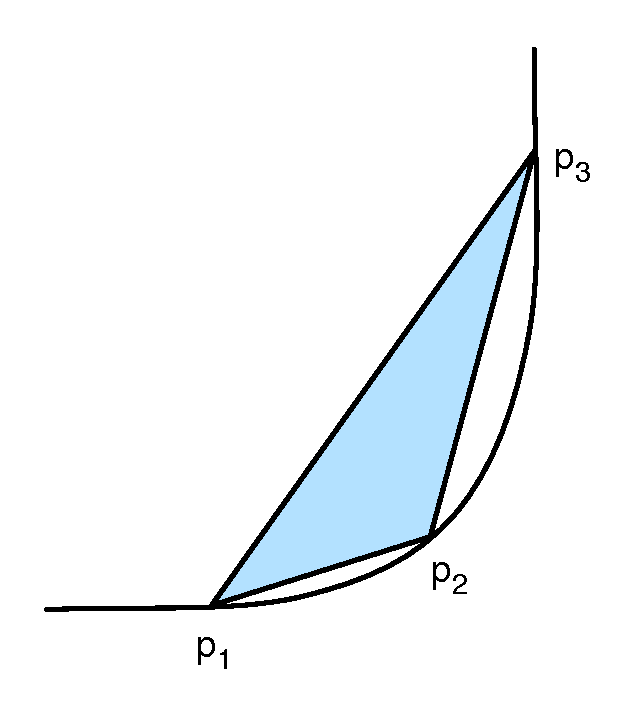
\includegraphics[width=0.35\textwidth]{img/convexhull.pdf}
\caption{Convex hull di $p_1,p_2,p_3$}
\label{fig:convexhull}
\end{center}
\end{figure}

Dalla definizione di funzione convessa e di convex hull, si può ricavare che data una funzione f convessa e comunque presi k punti $p_1,p_2,..p_k$ su y=f(x), risulta che $CH(p_1,p_2,...p_k)$ sta ``sopra`` y=f(x). L'esempio in figura \ref{fig:convexhull} mostra esattamente questo fatto con 3 punti (f è la curva).
Questo risultato è noto come disuguaglianza di Jensen. Tuttavia per arrivare alla forma ''finale`` della disuguaglianza, è necessario effettuare qualche passaggio a partire dall'idea che è stata appena esposta.

Potremo allora descrivere tutti gli infiniti punti del convex hull. Ovvero, data $f: [a,b] \to R$ convessa e comunque presi k punti 
$p_1,p_2,..p_k$ su y=f(x), risulta che:
\[
f(x) \le y, \forall P=(x,y) \in CH(p_1,p_2,...p_k)
\]
Stiamo in sostanza esprimendo il fatto che tutti i punti del convex hull stanno sopra la curva. Ma grazie alla \eqref{convex}, possiamo 
descrivere questi infiniti punti. Risulta dunque che:
\[
 P(x,y)=P \left (\sum_{i=1}^k \lambda_i x_i, \sum_{i=1}^k \lambda_i f(x_i) \right)  
                 \forall \bar{\lambda}=(\lambda_1,\lambda_2,...,\lambda_k) \in \Delta_k
\]

Possiamo ora arrivare alla versione finale della disuguaglianza.

\bigskip

\begin{teorema}[Disuguaglianza di Jensen]
 Sia $f: [a,b] \to R$ una funzione convessa, $x_1..x_k \in$ [a,b], $\bar{\lambda}=(\lambda_1,\lambda_2,...,\lambda_k) \in \Delta_k$.
 Allora vale che:
 \[
 f \left( \sum_{i=1}^k \lambda_i x_i \right) \le \sum_{i=1}^k \lambda_i f(x_i)
 \]
\begin{proof}
 Per prima cosa è necessario dimostrare che il teorema sia ''ben posto``, ovvero che f sia calcolata sempre 
 all'interno del dominio [a,b].
 Bisogna in sostanza dimostrare che:
 \[
  a \le x_i \le b  \ \ \forall i=1..k
 \]
 E che:
 \[
  a \le \sum_{i=1}^k \lambda_i x_i \le b \ \ \forall i=1..k
 \]

 \noindent
 Il primo caso è banale, infatti $x_1..x_k \in$ [a,b] per ipotesi.
 Per quanto riguarda il secondo caso invece osserviamo che $\lambda_i \ge0$ per ipotesi.
 Abbiamo quindi che:
 \[\begin{split}
  & a \le x_1 \le b \\
  \Rightarrow & \lambda_i a \le \lambda_i x_i \le \lambda_i b \\
  \Rightarrow & \sum_{i=1}^k \lambda_i a \le \sum_{i=1}^k \lambda_i x_i \le \sum_{i=1}^k \lambda_i b \\
  \Rightarrow & a \sum_{i=1}^k \lambda_i \le \sum_{i=1}^k \lambda_i x_i \le b \sum_{i=1}^k \lambda_i \\
  \Rightarrow & a \le \sum_{i=1}^k \lambda_i x_i \le b \\
   \end{split}
 \]
Il teorema è dunque ben posto. Possiamo allora iniziare la dimostrazione, per induzione su k (numero di punti).

\begin{description}
 \item[Caso base, k=2]
  \mbox{}

  Dobbiamo dimostrare che per ogni $\lambda_1,\lambda_2$ positivi, tali che $\lambda_1+\lambda_2=1$:
  \[
   f( \lambda_1 x_1 + \lambda_2 x_2) \le \lambda_1 f(x_1) + \lambda_2 f(x_2)
  \]
  Ma ciò è equivalente a:
  \[
   f( \lambda_1 x_1 + (1-\lambda_1) x_2) \le \lambda_1 f(x_1) + (1-\lambda_1) f(x_2)
  \]
  Che è banalmente vero, data la convessità di f.

 \item[Passo induttivo]
\mbox{}

Supponiamo che la disuguaglianza sia vera per k e dimostriamo che vale anche per k+1.
Pongo:
\[
 \mu_i=\frac{\lambda_i}{1-\lambda_{k+1}} \ i=1..k
\]
Osservo che $\mu_i>0 \forall i=1..k$ (rapporto di quantità positive) e che vale:
\[\begin{split}
 & \sum_{i=1}^k \mu_i=\sum_{i=1}^k \frac{\lambda_i}{1-\lambda_{k+1}} \\
 &= \frac{1}{1-\lambda_{k+1}} \sum_{i=1}^k \lambda_i
 = \frac{1-\lambda_{k+1}}{1-\lambda_{k+1}}=1
 \end{split}
\]
Considero ora la parte sinistra della disuguaglianza da dimostrare:
\[\begin{split}
 & f \left( \sum_{i=1}^{k+1} \lambda_i x_i \right) \\
 = & f \left( \sum_{i=1}^k \lambda_i x_i +\lambda_{k+1}x_{k+1} \right) \\
 = & f \left( \sum_{i=1}^k (1-\lambda_{k+1}) \mu_i x_i +\lambda_{k+1}x_{k+1} \right) \\
 = & f \left( (1-\lambda_{k+1}) \sum_{i=1}^k \mu_i x_i +\lambda_{k+1}x_{k+1} \right) \\
 \end{split}
\]

Ma poiché f è convessa (primo passaggio) e vale l'ipotesi induttiva (secondo passaggio):
\[\begin{split}
 & f \left( (1-\lambda_{k+1}) \sum_{i=1}^k \mu_i x_i +\lambda_{k+1}x_{k+1} \right) \\
 & \le (1-\lambda_{k+1})  f \left( \sum_{i=1}^k \mu_i x_i\right) +\lambda_{k+1} f(x_{k+1})  \\
 & \le (1-\lambda_{k+1})  \sum_{i=1}^k \mu_i f(x_i) +\lambda_{k+1} f(x_{k+1})  \\
 & = \sum_{i=1}^k \lambda_i f(x_i) +\lambda_{k+1} f(x_{k+1}) \\
 &= \sum_{i=1}^{k+1} \lambda_i f(x_i) \\
 \end{split}
\]

Riassumendo dunque abbiamo che:
\[
f \left( \sum_{i=1}^{k+1} \lambda_i x_i \right) \le \sum_{i=1}^{k+1} \lambda_i f(x_i)
\]

che dimostra il passo induttivo, concludendo la dimostrazione.
\end{description}
\end{proof}
\label{jensen}
\end{teorema}

\begin{corollario}
 Se inoltre f è strettamente convessa, vale che:
 \[
 f \left( \sum_{i=1}^k \lambda_i x_i \right) = \sum_{i=1}^k \lambda_i f(x_i) \iff \forall i \in \sigma(\bar{\lambda}) \ : \ x_i=const
 \]
 Dove $\sigma(\bar{\lambda})$ è detto supporto di $\bar{\lambda}$. Ovvero è l'insieme degli indici i per cui $\lambda_i \ne 0$
 \begin{proof}
 \mbox{}

  \begin{description}
   \item[\(\Longrightarrow\)] (Omesso, la dimostrazione è complicata)
   \item[\(\Longleftarrow\)] 
   Si ha che:
   \[\begin{split}
    & f \left( \sum_{i=1}^k \lambda_i x_i \right)=
    f \left( \sum_{i \in \sigma(\bar{\lambda}) } \lambda_i x_i \right) \\
    =& f \left( \sum_{i \in \sigma(\bar{\lambda}) } \lambda_i const \right)=
     f \left( const \sum_{i \in \sigma(\bar{\lambda}) } \lambda_i \right) \\
    =& f \left( const \right)= \sum_{i \in \sigma(\bar{\lambda}) } [\lambda_i] f \left( const \right) \\
    =& \sum_{i \in \sigma(\bar{\lambda}) } [\lambda_i f \left( const \right)] \\
    =& \left( \sum_{i=1}^k \lambda_i f(x_i) \right)
     \end{split}
   \]

  \end{description}
 \end{proof}
\end{corollario}

\bigskip

\noindent
Introduciamo ora il concetto di metrica (o distanza), al fine di descrivere una particolare distanza.

\begin{definizione}[Metrica]
 Dato un insieme X, una metrica (o distanza) è una funzione
\[
 d: X \times X \to R
\]
Per cui valgono le seguenti proprietà, $\forall x,y,z \in X$:
\[\begin{split}
 & 1) d(x,y) \ge 0 \\
 & 2) d(x,y)=0 \iff x=y \\
 & 3) d(x,y)=d(y,x) \\
 & 4) d(x,y) \le d(x,z)+d(z,y)
 \end{split}
\]
\end{definizione}

\begin{definizione}[Distanza di Kullback-Leibler]
\mbox{}

 Dati $\bar{p} \ e \ \bar{q} \in \Delta_n$, la lora distanza di Kullback-Leibler è:
\[
 D_{KL}(\bar{p} \| \bar{q})=\sum_{i=1}^n p_i log\frac{p_i}{q_i}
\]

(Assumiamo che $0 log0=0$ e $p_i log \frac{p_i}{0}=\infty$ )
\label{distkl}
\end{definizione}

\begin{osservazione}
 La distanza di Kullback-Leibler non è una metrica. Non valgono infatti le proprietà 3 e 4.
\end{osservazione}

\begin{teorema}
 La distanza di Kullback-Leibler soddisfa le proprietà 1 e 2 di metrica.
 Ovvero, date $\bar{p}$ e $\bar{q} \in \Delta_n$ (distribuzioni di probabilità):

 \begin{itemize}
  \item[(i)]  $D_{KL}(\bar{p} \| \bar{q}) \ge 0$
  \item[(ii)] $D_{KL}(\bar{p} \| \bar{q}) = 0 \iff \bar{p}=\bar{q}$
 \end{itemize}

\begin{proof}
 \mbox{}

 \begin{description}
 \item[(i)]
  \[\begin{split}
    &-D_{KL}(\bar{p} \| \bar{q})= -\sum_{i=1}^n p_i log \frac{p_i}{q_i} \\
    &=\sum_{i=1}^n p_i log \frac{q_i}{p_i} \\
    &=\sum_{i \in \sigma(\bar{p})} p_i log \frac{q_i}{p_i} \\
    \end{split}
  \]
  Ora posso applicare la disuguaglianza di Jensen (teorema \ref{jensen}). Tuttavia 
  il verso della disuguaglianza sarà inverso, in quanto la funzione logaritmo è concava e non convessa.
 \[\begin{split}
  &\sum_{i \in \sigma(\bar{p})} p_i log \frac{q_i}{p_i} \\
   \le & log \sum_{i \in \sigma(\bar{p})} p_i \frac{q_i}{p_i} \\
  =& log \sum_{i \in \sigma(\bar{p})} q_i \\
  \le & log \sum_{i=1}^n q_i \\
  =& log 1=0
  \end{split}
 \]

  Abbiamo quindi dimostrato che:
  \[
   -D_{KL}(\bar{p} \| \bar{q}) \le 0
  \]
  Da cui:
  \[
   D_{KL}(\bar{p} \| \bar{q}) \ge 0
  \]
 \item[(ii)]
  Possiamo utilizzare quanto dimostrato nel punto (i). In particolare, la distanza sarà zero se e solo se 
  le due disuguaglianze che compaiono sono uguaglianze.
  Per quanto riguarda la seconda disuguaglianza:
  \[\begin{split}
   &log \sum_{i \in \sigma(\bar{p})} q_i=log \sum_{i=1}^n q_i \\
   \iff &\sum_{i \in \sigma(\bar{p})} q_i=\sum_{i=1}^n q_i \\
   \iff & \forall i \notin \sigma(\bar{p}) : p_i=q_i
   \end{split}
  \]
   Ciò è vero in quanto, affinché i due termini coincidano, al di fuori del supporto di p non devono esserci indici i per cui 
   $q_i \ne 0$ (altrimenti la sommatoria ''completa`` sarebbe più grande ristretto a quella limitata al supporto di p).
   Ma se i non appartiene al supporto di p, allora $p_i=0$. Pertanto deve essere $p_i=q_i=0$, per $i \notin \sigma(\bar{p})$.

   Per quanto riguarda invece la prima disuguaglianza, si avrà uguaglianza solamente nel caso limite dato dal corollario al teorema 
   di Jensen (si noti che la funzione logaritmo è strettamente concava).
   Per il corollario bisogna avere che:
   \[
    \forall i \in \sigma(\bar{\lambda}) \ : \ x_i=const
   \]
   Nel caso in esame dunque:
   \[
    \forall i \in \sigma(\bar{p}) \ : \ \frac{q_i}{p_i}=const
   \]
   Quindi:
   \[
    \forall i \in \sigma(\bar{p}) \ : q_i=const \ p_i
   \]

   Da cui:
   \[ \begin{split}
    \sum_{i \in \sigma(p)} q_i &=\sum_{i \in \sigma(p)} const \ p_i \\
     &=const \sum_{i \in \sigma(p)} p_i \\
     &=const=1
    \end{split}
   \]
   Quindi deve essere const=1, ovvero:
   \[
    \forall i \in \sigma(\bar{p}) \ : p_i=q_i
   \]
   Riassumendo quindi le due condizioni si ha uguaglianza se e solo se:
   \[
    \forall i=1..n : p_i=q_i \ \ \iff \ \ \bar{p}=\bar{q}
   \]

\end{description}

\end{proof}
\label{leibler}
\end{teorema}

La distanza di Kullback-Leibler è anche nota come \textit{entropia relativa} e misura in un certo senso la distanza tra due distribuzioni di probabilità. Vediamo ora il concetto, molto importante, di informazione mutua (che è una particolare distanza di Kullback-Leibler).

\begin{definizione}[Informazione mutua]
 Date X,Y v.a e posto al solito $p(x)=Pr\{X=x\}$, $p(y)=Pr\{Y=y\}$, $p(x,y)=Pr\{X=x, Y=y\}$ si definisce 
 informazione mutua:
 \[
  I(X;Y)=\sum_{x \in X} \sum_{y \in Y} p(x,y) log \frac{p(x,y)}{p(x)p(y)}
 \]
\end{definizione}

\begin{osservazione}
 L'informazione mutua è una specifica distanza di Kullback-Leibler: $D_{KL}(p(x,y) \|  p(x)p(y))$.
 \begin{proof}
  Bisogna innanzitutto verificare che p(x)p(y) sia una distribuzione di probabilità.
  In maniera banale (prodotto di due probabilità):
  \[
   0 \le p(x)p(y) \le 1 \ \ \forall x \in X,y \in Y
  \]
  Risulta poi:
  \[\begin{split}
   &\sum_{x \in X}\sum_{y \in Y} p(x)p(y) \\
   =&\sum_{x \in X} p(x) \sum_{y \in Y}p(y) \\
   =& 1 \times 1 \\
   =&1 
    \end{split}
  \]
  p(x)p(y) è dunque una distribuzione di probabilità.
  Ponendo $p_i=p(x,y)$ e $q_i=p(x)p(y)$, si ottiene la distanza KL.
 \end{proof}

\end{osservazione}

In sostanza quindi, l'informazione mutua misura in un certo senso il grado di dipendenza tra due v.a.
Se infatti le due variabili sono indipendenti, allora p(x,y)=p(x)p(y) e quindi l'informazione mutua vale zero. Viceversa, più le 
variabili sono dipendenti tra loro, più la distanza aumenta. Vediamo ora come l'informazione mutua sia strettamente legata 
al concetto di entropia.

\begin{teorema}
\[
 I(X;Y)=H(X)-H(X/Y)=H(Y)-H(Y/X)
\]
\begin{proof}
\[\begin{split}
 I(X;Y)=&\sum_{x \in X} \sum_{y \in Y} p(x,y) log \frac{p(x,y)}{p(x)p(y)} \\
   =&\sum_{x \in X} \sum_{y \in Y} p(x,y) log \frac{p(y)p(x/y)}{p(x)p(y)} \\
   =&\sum_{x \in X} \sum_{y \in Y} p(x,y) log \frac{p(x/y)}{p(x)} \\
   =&\sum_{x \in X} \sum_{y \in Y} p(x,y) log (p(x/y))-\sum_{x \in X} \sum_{y \in Y} p(x,y) log (p(x)) \\
   =&-H(X/Y)-\sum_{x \in X} log (p(x)) \sum_{y \in Y} p(x,y)\\
   =&-H(X/Y)-\sum_{x \in X} log (p(x)) p(x)\\
   =&-H(X/Y)+H(X)\\
   =&H(X)-H(X/Y)\\
 \end{split}
\]
In maniera del tutto analoga si dimostra la seconda uguaglianza.
\end{proof}
\label{infmutua}
\end{teorema}

In sostanza quindi l'informazione mutua può anche essere vista come differenza di entropie. Utilizzando, ad esempio, la prima 
uguaglianza l'informazione mutua tra X e Y mi dice l'incertezza che mi rimane sulla variabile X, dopo aver ''conosciuto`` la variabile 
Y. Come si vedrà più avanti, questo fatto costituisce la base per l'analisi dei canali di trasmissione (nello specifico è fondamentale 
per calcolare la capacità di un canale).

\begin{osservazione}
 I(X;Y)=H(X)+H(Y)-H(X,Y)
 \begin{proof}
  Per il teorema \ref{infmutua}:
  \[
  I(X;Y)=H(X)-H(X/Y)
  \]
  Per la regola della catena (Teorema \ref{catena}):
  \[\begin{split}
  I(X;Y)&=H(X)-[H(X,Y)-H(Y)] \\
        &=H(X)+H(Y)-H(X,Y)
    \end{split}
  \]
 \end{proof}
\end{osservazione}

Si può utilizzare un diagramma di Venn, per rappresentare (in maniera intuitiva) la relazione tra entropia ed informazione mutua (Figura \ref{fig:mutua}).

\begin{figure}[htbp]
\begin{center}
	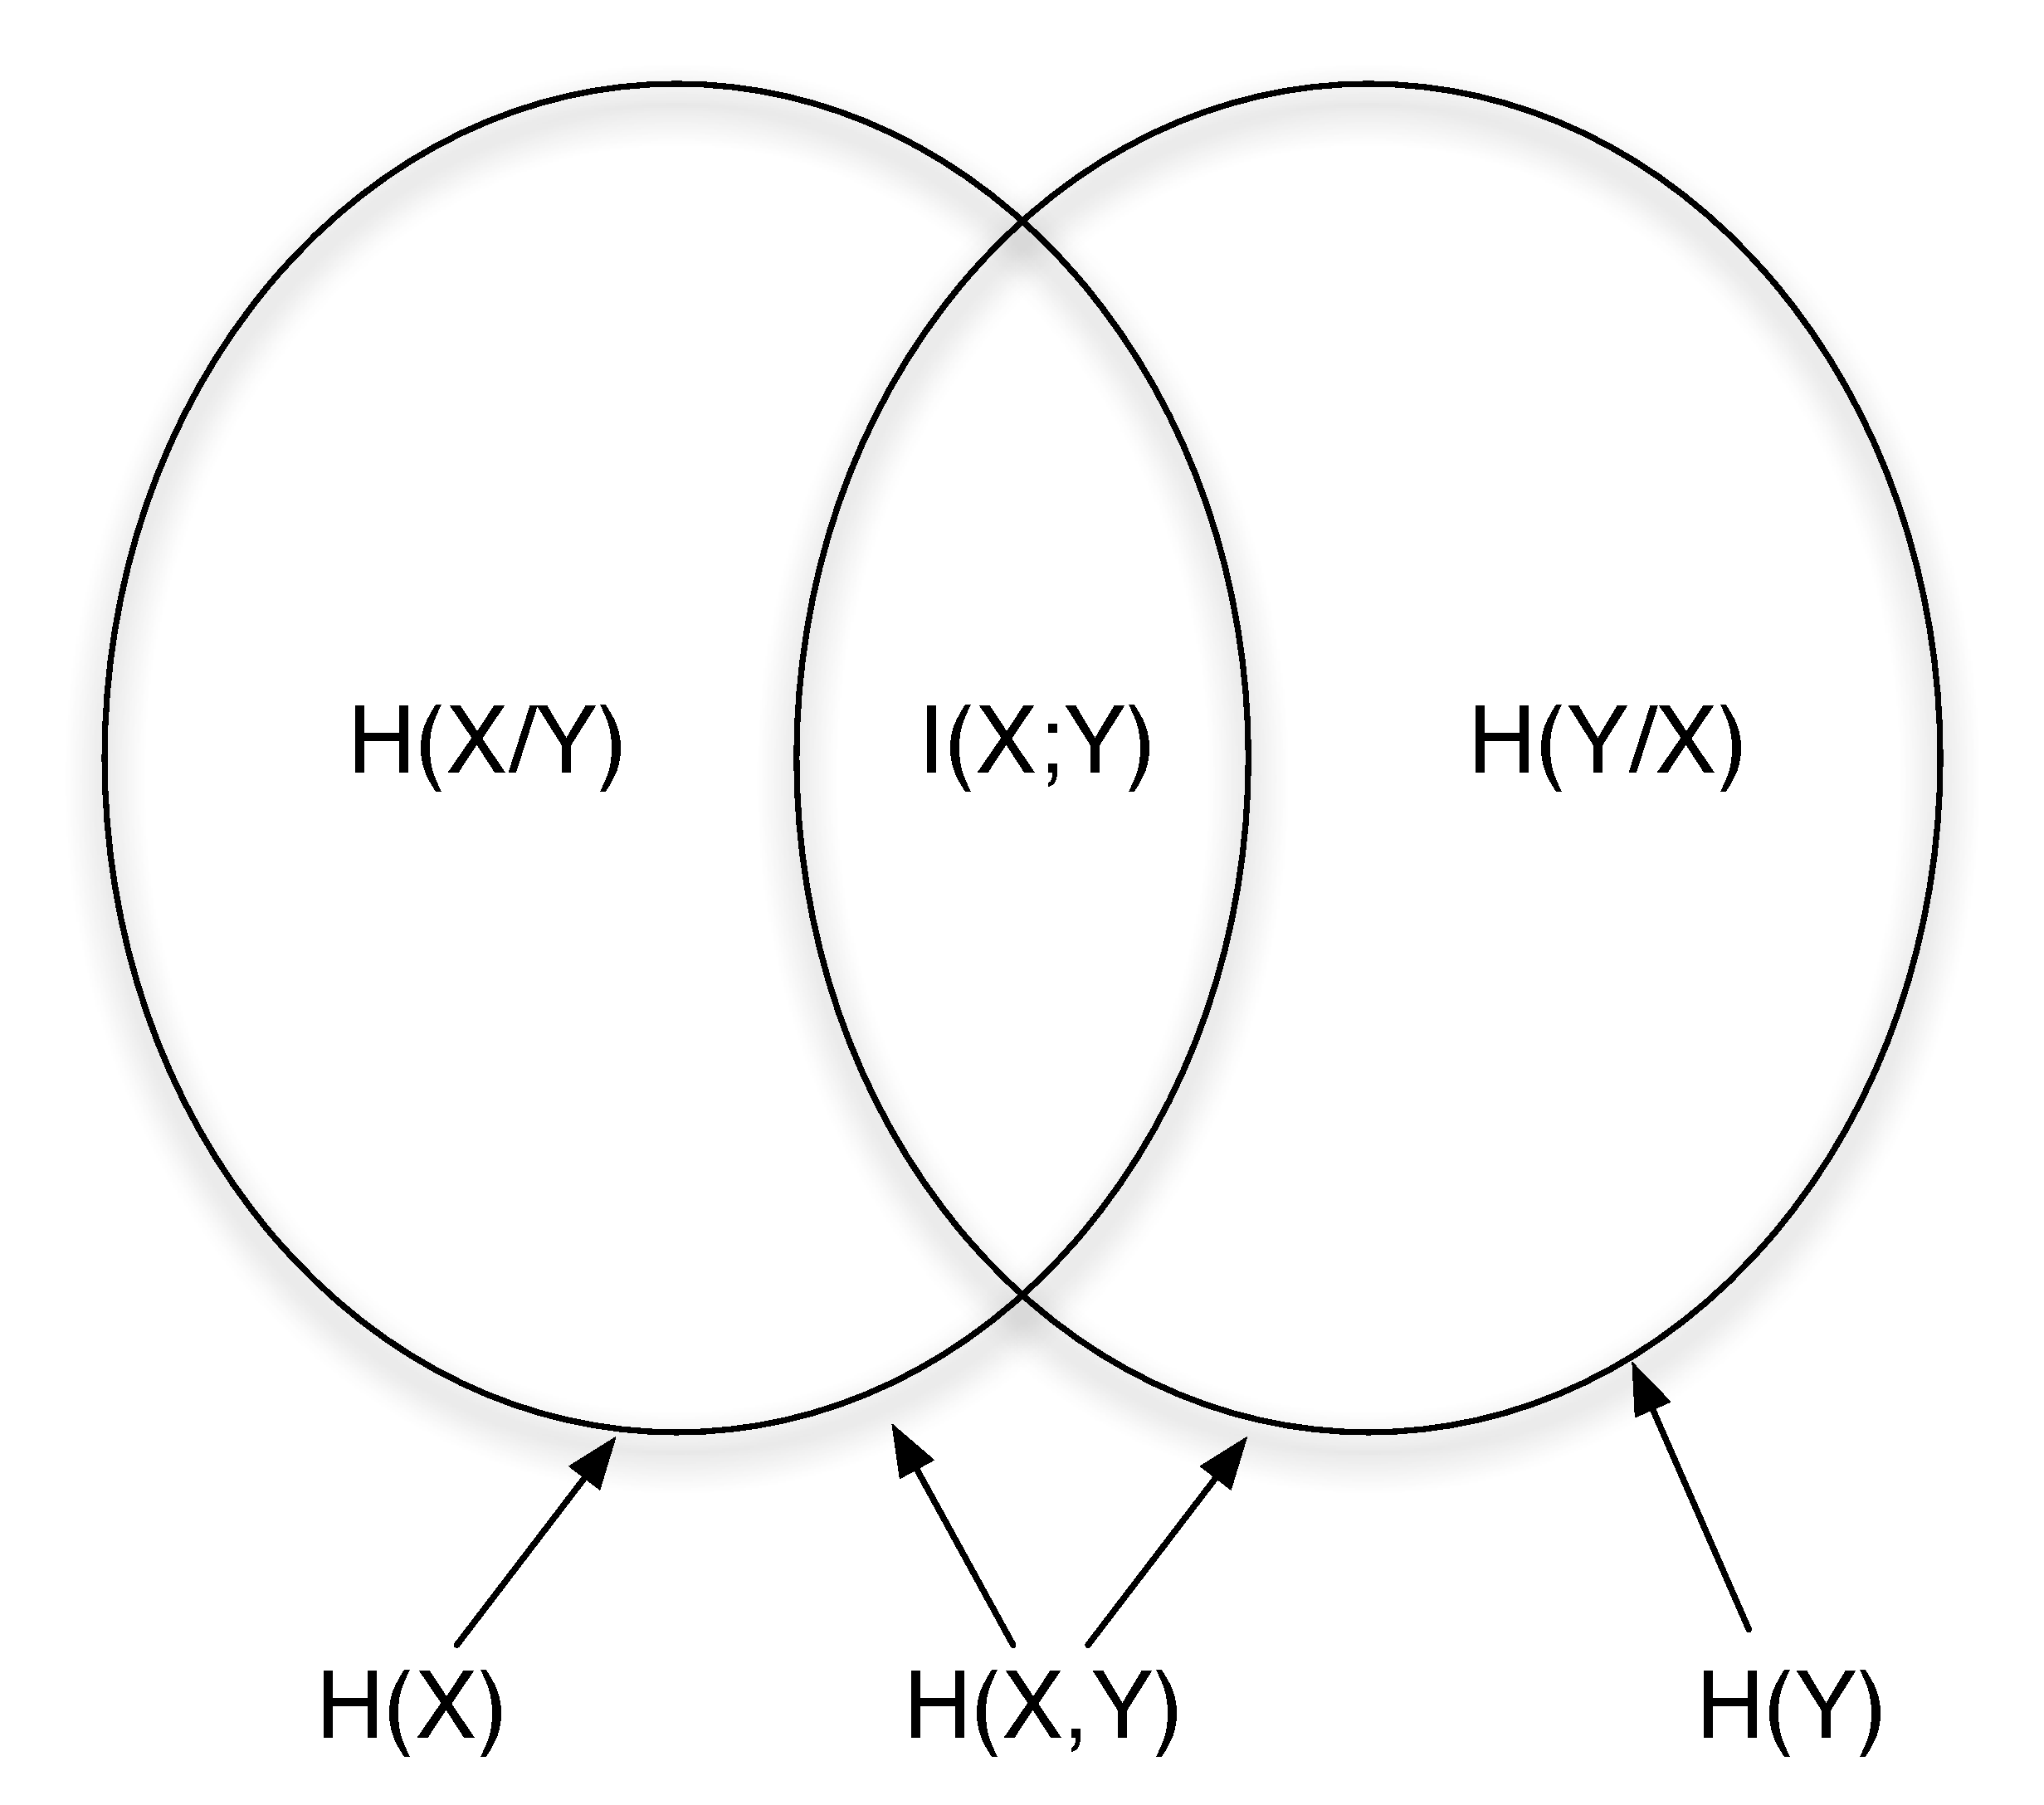
\includegraphics[width=0.5\textwidth]{img/mutua.pdf}
\caption{Relazione tra entropia ed informazione mutua}
\label{fig:mutua}
\end{center}
\end{figure}

\noindent
Possiamo, sempre sulla base del teorema \ref{infmutua}, effettuare una serie di osservazioni sull'informazione mutua.

\begin{osservazione}
\[
 I(X;X)=H(X)
\]
\end{osservazione}

\begin{osservazione}
 \[
   I(X;Y) \ge 0  
 \]
 \begin{proof}
  Banale, poiché l'informazione mutua è una distanza KL che è maggiore o uguale a 0 per il teorema \ref{leibler}.
 \end{proof}
\label{distinf}
\end{osservazione}

\begin{osservazione}
 \[
   I(X;Y)=0 \iff X \ e \ Y \ sono \ statisticamente \ indipendenti  
 \]
 \begin{proof}
  Per il teorema \ref{leibler} una distanza KL è 0 se e solo se le due distribuzioni di probabilità coincidono.
  In questo caso quindi, se e solo se p(x,y)=p(x)p(y) (che è proprio la definizione di indipendenza).
 \end{proof}
 \label{mutuaindip}
\end{osservazione}

\begin{osservazione}[Il condizionamento riduce l'entropia]
 \[
  H(X/Y) \le H(X)
 \]
  \begin{proof}
   \[\begin{split}
     & H(X/Y) \le H(X) \\ 
     \iff & H(X/Y) -H(X) \le 0 \\
     \iff & H(X)-H(X/Y) \ge 0 \\
     \iff & I(X;Y) \ge 0
     \end{split}
   \]
  Ma per l'osservazione \ref{distinf}, l'informazione mutua è sempre maggiore o uguale a zero.
  \end{proof}

 \label{condizionamento}
\end{osservazione}

\begin{osservazione}
 La funzione entropia è concava. Ovvero dati:
 \[
 \bar{p} \in \Delta_n \\
 H(\bar{p})=-\sum_{i=1}^n p_i log(p_i)
 \]
 Vale che:
 \[
  \forall \lambda \in [0,1] \ e \ \bar{p}_1,\bar{p}_2 \in \Delta_n \ : \ 
   H(\lambda \bar{p}_1 + (1-\lambda) \bar{p}_2) \ge \lambda H(\bar{p}_1) + (1-\lambda) H(\bar{p}_2)
 \]

\begin{proof}
 Consideriamo $\X=\{1..n\}$ e costruiamo due variabili casuali $X_1,X_2$ con valori in $\X$, così distribuite:
 \[
  X_1 \sim \bar{p_1} \\ X_2 \sim \bar{p_2}
 \]
 Consideriamo poi una variabile $\Theta$ nell'insime $\{1,2\}$, così distribuita:
 \[
  Pr\{\Theta=1\}=\lambda \\ Pr\{\Theta=2\}=1-\lambda
 \]
 Costruiamo infine una variabile Z che varia nell'insieme X, definita come:
 \[
  Z=X_{\Theta}
 \]
 In altre parole Z è una variabile composta, che vale $X_1$ con probabilità $\lambda$ e $X_2$ con probabilità $1-\lambda$.
 Ora analizziamo la distribuzione Z, calcolando $Pr\{Z=x\} , \ x \in X$:
 \[\begin{split}
  Pr\{Z=x\}=&Pr\{[\Theta=1 \land X_1=x] \lor [\Theta=2 \land X_2=x]  \} \\
  =&Pr\{[\Theta=1 \land X_1=x]\} + Pr\{[\Theta=2 \land X_2=x]  \} \\
  =&Pr\{\Theta=1\} Pr\{X_1=x\} + Pr\{\Theta=2\} Pr\{X_2=x\} \\
  =& \lambda \bar{p}_{1x} + (1-\lambda) \bar{p}_{2x}
  \end{split}
 \]
  Dove con $\bar{p}_{1x}$ abbiamo indicato la componente x° di $\bar{p}_1$ (similmente per $\bar{p}_2$).
  Risulta quindi che:
  \[
   Z \sim q=\lambda \bar{p}_1 + (1-\lambda) \bar{p}_2
  \]
  Da cui:
  \[
   H(Z)=H(\lambda \bar{p}_1 + (1-\lambda) \bar{p}_2)
  \]
  Ora semplifichiamo $H(Z/\Theta)$. Risulta:
  \[\begin{split}
   H(Z/\Theta)=&Pr\{\Theta=1\}H(Z/\Theta=1)+Pr\{\Theta=2\}H(Z/\Theta=2) \\
   =& \lambda H(Z/\Theta=1)+(1-\lambda)H(Z/\Theta=2) \\
   =& \lambda H(X_1)+(1-\lambda)H(X_2) \\
   =& \lambda H(\bar{p}_1)+(1-\lambda)H(\bar{p}_2) \\
   \end{split}
  \]
  Riassumendo si ha dunque che:
  \[
    H(Z)=H(\lambda \bar{p}_1 + (1-\lambda) \bar{p}_2) \\ H(Z/\Theta)=\lambda H(\bar{p}_1)+(1-\lambda)H(\bar{p}_2)
  \]
  Ora, per l'osservazione \ref{condizionamento} il condizionamento riduce l'entropia. Vale quindi:
   \[
     H(Z/\Theta) \le H(Z) 
  \]
  Ovvero:
  \[\begin{split}
   & H(Z/\Theta) \le H(Z) \\
   \iff & H(Z) \ge H(Z/\Theta)  \\
   \iff &  H(\lambda \bar{p}_1 + (1-\lambda) \bar{p}_2) \ge \lambda H(\bar{p}_1)+(1-\lambda)H(\bar{p}_2)
   \end{split}
  \]


\end{proof}
\label{entrconcava}
\end{osservazione}

In maniera analoga a quanto fatto per l'entropia, cerchiamo ora di definere l'informazione mutua condizionata.
Vogliamo in sostanza calcolare:
\[
 I(X,Y/Z)
\]
Al solito, calcoliamo prima il valore per uno specifico $z \in Z$:
\[\begin{split}
 I(X,Y/Z=z)&=D_{KL}[p(x,y/z) \ \| \ p(x/z)p(y/z)] \\
 &=\sum_{x \in X} \sum_{y \in Y} p(x,y/z) log \frac{p(x,y/z)}{p(x/z)p(y/z)}
  \end{split}
\]

\noindent
Calcoliamo poi (sempre come già fatto per l'entropia) il valore atteso rispetto a Z:
\[
 \begin{split}
 I(X,Y/Z)&=\sum_{z \in Z} p(z) I(X,Y/Z=z) \\
 &=\sum_{z \in Z} \sum_{x \in X} \sum_{y \in Y} p(z)p(x,y/z) log \frac{p(x,y/z)}{p(x/z)p(y/z)} \\
 &=\sum_{z \in Z} \sum_{x \in X} \sum_{y \in Y} p(x,y,z) log \frac{p(x,y/z)}{p(x/z)p(y/z)}
  \end{split}
\]

\bigskip
\noindent
Naturalmente non siamo in presenza di una forma ''compatta``. Tuttavia a partire da questo risultato, 
si può arrivare alla seguente osservazione.

\begin{osservazione}
 \[
 I(X,Y/Z)=H(X/Z)-H(X/Y,Z)
\]
\end{osservazione}

\begin{osservazione}
 \[
  I(X,Y/Z) \ge 0
 \]
\end{osservazione}

\begin{osservazione}
\[
 H(X_1,X_2,..,X_n)=\sum_{i=1}^n H(X_i/X_1,X_2,..X_{i-1}) \le \sum_{i=1}^n H(X_i)
\]
\end{osservazione}


\section{Asymptotic Equipartition Property}
\label{aep}
La AEP (Asymptotic Equipartition Property) è la variante della legge dei grandi numeri, nel campo della teoria dell'informazione.
La legge (debole) dei grandi numeri, importante risultato nel campo della statistica, può essere riassunta nel modo seguente.

Siano $Z_1..Z_n$ delle variabili aleatorie i.i.d (indipendenti e identicamente distribuite) ciascuna con media $\mu$ e varianza $\sigma^2$.
Sia inoltre $\bar{Z}_n$ la media campionaria di queste n variabili, ovvero:
\[
 \bar{Z}_n=\frac{1}{n} \sum_{i=1}^n Z_i
\]

Allora vale che:
\[
 \forall \epsilon > 0: \\
 \lim_{n\to\infty}Pr(|\bar{Z}_n-\mu|\le \epsilon)=1
\]

Possiamo in sostanza dire che (per n grande) la media campionaria tende in probabilità al valore atteso.

Siano ora $X_1..X_n$ delle variabili aleatorie i.i.d. Indichiamo con $X^n$ l'insieme di tutte le sequenze possibili e con $\bar{x}=(x_1,x_2,...x_n) \in X^n $ una generica sequenza.

\bigskip
\noindent
\textbf{Esempio}

\noindent
Siano $A_1$ e $A_2$ due v.a. i.i.d, definite nell'insieme $\{1,2,3\}$.
Allora:
\[
 A^2=\Bigl \lbrace \{1,1\},\{1,2\},\{1,3\},\{2,1\},\{2,2\},\{2,3\},\{3,1\},\{3,2\},\{3,3\} \Bigl \rbrace
\]
Una generica sequenza $\bar{a}$ è (ad esempio) $\{2,3\}$.

\bigskip
Possiamo dividere l'insieme $X^n$ in due parti: l'insieme delle sequenze tipiche e l'insieme delle sequenza atipiche.

\begin{definizione}
 L'insieme delle sequenze ($\epsilon$,n)-tipiche è:
\[
 A_{\epsilon}^n=\{ \bar{x} \in X^n \mid 2^{-n(H(x)+\epsilon)} \le p(\bar{x}) \le 2^{-n(H(x)-\epsilon)} \}
\]
\label{tipiche}
\end{definizione}

\noindent
Stiamo in sostanza affermando che le sequenze tipiche hanno tutte circa la stessa probabilità: 
$p(\bar{x}) \backsimeq 2^{-nH(x)} \ \forall \bar{x} \in A_{\epsilon}^n$

\begin{teorema}[AEP]
 \[
  \lim_{n \to \infty} Pr\{A_{\epsilon}^n\}=1
 \]
 \begin{proof}
  \[
  \begin{split}
    \bar{x} \in A_{\epsilon}^n &\iff 2^{-n(H(x)+\epsilon)} \le p(\bar{x}) \le 2^{-n(H(x)-\epsilon)} \\
    &\iff -n(H(x)+\epsilon) \le log(p(\bar{x})) \le -n(H(x)-\epsilon) \\
    &\iff -(H(x)+\epsilon) \le \frac{1}{n} log(p(\bar{x})) \le -(H(x)-\epsilon) \\
    &\iff H(x)-\epsilon \le -\frac{1}{n} log(p(\bar{x})) \le H(x)+\epsilon \\
    &\iff \mid -\frac{1}{n} log(p(\bar{x})) - H(x) \mid \le \epsilon  \\
  \end{split}
  \]

 Consideriamo ora $Z_1..Z_n$ v.a. i.i.d e poniamo
 \[
  Z_i= -log( p(X_i) )
 \]
 
  \noindent
  Calcoliamo allora la media campionaria delle variabili Z:
  \[
  \begin{split}
   \bar{Z}_n &=\frac{1}{n} \sum_{i=1}^n Z_i \\
             &=\frac{1}{n} \sum_{i=1}^n -log(p(X_i)) \\
             &=-\frac{1}{n} log \left [ \prod_{i=1}^n (p(X_i) \right] \\
             &=-\frac{1}{n} log(p(\bar{x}))
  \end{split}
  \]
  L'ultimo passaggio è dovuto all'indipendenza delle variabili.
  Consideriamo ora il valore atteso delle variabili Z:
  \[
  \begin{split}
   \mu &=\sum_{i=1}^n p(Z_i) Z_i \\
        &=\sum_{i=1}^n p(X_i)(-log(p(X_i)) \\
             &=H(X)
  \end{split}
  \]
  Risulta quindi:
  \[ \begin{split}
   \bar{x} \in A_{\epsilon}^n &\iff \mid -\frac{1}{n} log(p(\bar{x})) - H(x) \mid \le \epsilon \\
   &\iff \mid \bar{Z}_n - \mu \mid \le \epsilon
    \end{split}
  \]
  Da cui, per la legge dei grandi numeri:
  \[
  \lim_{n \to \infty} Pr\{A_{\epsilon}^n\}=
     \lim_{n \to \infty} Pr\{ \mid \bar{Z}_n - \mu \mid \le \epsilon \}=1
 \]

 \end{proof}

\end{teorema}

Per chiarire meglio i concetti esposti, possiamo rappresentare graficamente l'insieme $X^n$ delle sequenze, che 
contiene quelle tipiche e quelle atipiche (figura \ref{fig:sequenze}).
Si nota come si tratti di due insiemi disgiunti. Il teorema AEP ci dice che, per n sufficientemente grande, la probabilità 
di avere una sequenze tipica tende a 1. Inoltre, tutte le sequenze tipiche sono circa equiprobabili.

\begin{figure}[htbp]
\begin{center}
	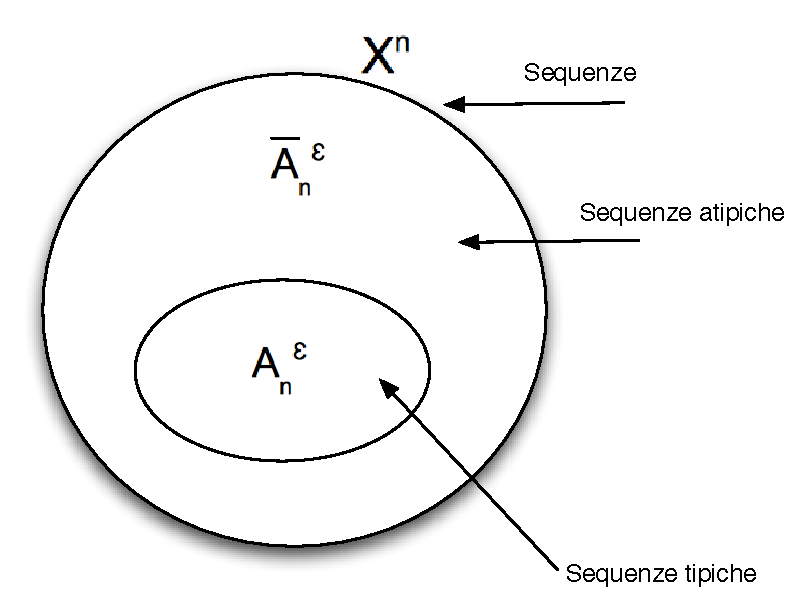
\includegraphics[width=0.6\textwidth]{img/sequenze.pdf}
\caption{Rappresentazione grafica delle sequenze}
\label{fig:sequenze}
\end{center}
\end{figure}

\bigskip
\noindent
\textbf{Esempio}

\noindent
Consideriamo il lancio di una moneta. Supponiamo di effettuare n lanci (con n grande) e costruire quindi sequenze lunghe n.
Se la moneta è totalmente sbilanciata ed esce sempre testa (probabilità di avere testa 1, di croce 0), allora ci sarà solo una sequenza
tipica: quella formata da tutte teste. Le altre sequenze infatti non potranno mai verificarsi.
Se la moneta è invece perfettamente bilanciata (probabilità di avere testa uguale a probabilità di avere croce) tutte le sequenze 
saranno tipiche. E' facile infatti notare che sono tutte equiprobabili.

\bigskip
E' interessante a questo punto sapere quanti elementi contiene l'insieme delle sequenze tipiche. Intuitivamente (per n suff. grande) la
sua cardinalità dovrebbe essere $2^{nH(x)}$. Infatti $1/2^{-nH(x)}=2^{nH(x)}$ poiché la probabilità totale è 1 e tutte le sequenze 
tipiche sono equiprobabili.

\bigskip
\noindent
\textbf{Esempio}

\noindent
Riprendiamo l'esempio della moneta considerato prima e proviamo a calcolare la cardinalità dell'insieme sequenze tipiche.
Per quanto detto il numero delle sequenze tipiche dovrebbe essere $2^{nH(x)}$.
Nel caso in cui la moneta è bilanciata, l'entropia risulta:
\[
 H(X)=H \left( \frac{1}{2},\frac{1}{2} \right)=1
\]
Quindi la cardinalità sarebbe $2^n$, ovvero tutte le sequenze sono tipiche (la cardinalità di $X^n$ è banalmente $2^n$).
Se consideriamo invece la moneta in cui la probabilità di avere testa è 1, allora l'entropia risulta:
\[
 H(X)=H \left(1\right)=0
\]
Quindi la cardinalità dovrebbe essere $2^{n0}=1$, ovvero esiste un'unica sequenza tipica.

\bigskip
Quanto detto finora è solo un ragionamento intuitivo, formalizziamo in maniera più accurata questo punto tramite alcune 
proposizioni.

\begin{osservazione}
 \[
   \forall \epsilon > 0, \ \exists n_0 \mid \forall n \ge n_0 \ : \ Pr\{A_{\epsilon}^n\} \ge 1 - \epsilon 
 \]
  
  \begin{proof}
   Una successione $\{a_n\}$ ha limite l $\in$ R se $\forall \delta > 0$: 
   \[
    \exists n_o \mid \forall n \ge n_0 : \ \mid a_n-l \mid \le \delta
   \]

   Ma per il teorema AEP:
   \[ \begin{split}
    & \lim_{n \to \infty} Pr\{A_{\epsilon}^n\}=1 \\
    & \Rightarrow \mid Pr\{A_{\epsilon}^n\} -1 \mid \le \delta \\
    & \Rightarrow 1- Pr\{A_{\epsilon}^n\} \le \delta \\
    & \Rightarrow Pr\{A_{\epsilon}^n\} \ge 1- \delta
    \end{split}
   \]
   Poniamo $\delta=\epsilon$ per concludere la dimostrazione.
  \end{proof}
\label{ossAep}
\end{osservazione}

\begin{proposizione}
 \mbox{}
 \begin{itemize}
  \item[(i)] $ |A_{\epsilon}^n| \le 2^{n(H(x)+\epsilon)}$
 
  \item[(ii)] $|A_{\epsilon}^n| \ge (1-\epsilon) 2^{n(H(x)-\epsilon)}$  (per n suff. grande)
 \end{itemize}
 \begin{proof}
  \mbox{}
  \begin{itemize}
   \item[(i)] Si ha che:
   \[
    1=\sum_{x \in X^n} p(x) \ge \sum_{x \in A_{\epsilon}^n} p(x) \ge 
      \sum_{x \in A_{\epsilon}^n} 2^{-n(H(x)+ \epsilon)}=|A_{\epsilon}^n| 2^{-n(H(x)+ \epsilon)} 
   \]
   Da cui:
   \[
    |A_{\epsilon}^n| 2^{-n(H(x)+ \epsilon)} \le 1 \Rightarrow |A_{\epsilon}^n| \le 2^{n(H(x)+ \epsilon)}
   \]


   \item[(ii)]
   Per l'osservazione \ref{ossAep}:
   \[
    \forall \epsilon > 0, \ \exists n_0 \mid \forall n \ge n_0 \ : \ 1 - \epsilon \le Pr\{A_{\epsilon}^n\}
   \]
   Da cui:
   \[
    1 - \epsilon \le Pr\{A_{\epsilon}^n\}=\sum_{x \in A_{\epsilon}} p(x) \le 
    \sum_{x \in A_{\epsilon}} 2^{-n(H(x)-\epsilon)} = |A_{\epsilon}^n| 2^{-n(H(x)-\epsilon)}
   \]
   Risulta quindi:
   \[\begin{split}
    & 1 - \epsilon \le |A_{\epsilon}^n| 2^{-n(H(x)-\epsilon)}  \\
    & \Rightarrow |A_{\epsilon}^n| 2^{-n(H(x)-\epsilon)}  \ge 1 - \epsilon \\
    &\Rightarrow |A_{\epsilon}^n| \ge (1 - \epsilon) 2^{n(H(x)-\epsilon)}
    \end{split}
   \]

  \end{itemize}

 \end{proof}

\end{proposizione}

Ques'ultima proposizione dimostra che la nostra intuizione era corretta e formalizza in maniera precisa all'interno 
di quali estremi si trova la cardinalità dell'insieme delle sequenze tipiche.

\subsection{Generalizzazione dell'AEP}

L'AEP fornisce dei risultati importanti, tuttavia ha delle ipotesi abbastanza restrittive. In particolare, abbiamo supposto che le v.a. 
$X_1..X_n$, fossero i.i.d. Nel caso di una sorgente generica, ciò equivale a dire che essa è senza memoria. Non sempre però è lecito fare questa assunzione. Per fare un esempio, se la sorgente emette delle lettere che costituiscono parole in lingua italiana, dopo la lettera e.g. h, seguirà con tutta probabilità una vocale. In questo contesto quindi non si potrebbe accettare l'ipotesi di indipendenza e non si potrebbe dunque applicare l'AEP.

Mettiamoci dunque in un caso più generale, considerando un processo stocastico. Possiamo pensare ad un processo stocastico, come ad una famiglia di variabili casuali $X_1..X_n$. Indicheremo tale processo nel seguente modo:
\[
 \{X_t\}_{t=1..\infty}
\]

In questo contesto possiamo pensare al processo come ad una sorgente, che genera appunto $X_1..X_n$. Ora, a seconda delle relazioni 
tra le variabili, possiamo avere diversi tipi di processi. Consideriamo i seguenti casi:
\begin{itemize}
 \item $X_1..X_n$ i.i.d. E' il caso che abbiamo considerato fino ad ora, in cui le variabili sono indipendenti
 \item Catena di Markov: E' un processo stocastico, per cui vale la seguente proprietà:
  \[\begin{split}
   &Pr\{ X_n=x_n \mid X_1=x_1 \mid X_2=x_2 \mid ... \mid X_{n-1}=x_{n-1}\} \\
   =&Pr\{ X_n=x_n \mid X_{n-1}=x_{n-1} \}
  \end{split}
  \]
  In sostanza quindi l'emissione di un simbolo (pensando in termini di sorgente), equivale unicamente all'emissione del simbolo 
  precedente. Si può dire in sostanza che la catena è di ordine 1 (è rilevante infatti solo l'ultimo simbolo emesso).
 \item Processo stazionario: E' un processo stocastico, per cui vale la seguente proprietà:
 \[\begin{split}
  \forall l \in Z: \\ & Pr\{X_1=x_1, X_2=x_2, ... , X_n=x_n\}  \\
  = &Pr\{X_{1+l}=X_1, X_{2+l}=x_2, ... , X_{n+l}=x_n \}
    \end{split}
 \]
  In questo caso quindi si ha una condizione ``relativa'' del tempo. Ovvero la probabilità di una certa sequenza non dipende dallo
  specifico istante temporale.
 \item Processo ergodico: Dato un processo stocastico, definiamo:
 \[
  N_{\bar{x}}^n(X_1X_2...X_n) 
 \]
  Come il numero di volte in cui compare la stringa $\bar{x}$ in $X_1X_2...X_n$.
  Allora un processo è ergodico se:
 \[
  \forall \bar{x} \in X^n: \frac{1}{n} N_{\bar{x}}^n(X_1X_2...X_n) \xrightarrow{n \to \infty} p(\bar{x}) \ in \ probabilita'
 \]
  Dove ``in probabilità'' equivale a dire:
  \[
   \forall \epsilon > 0: \lim_{n \to \infty} Pr\{ \mid \frac{1}{n} N_{\bar{x}}^n(X_1X_2...X_n) - p(\bar{x})  \mid \le \epsilon\}=1
  \]


\end{itemize}

Possiamo ora generalizzare il concetto di entropia, nel caso di un processo stocastico. Considerando quindi una serie di v.a. invece 
di un'unica variabile (com'era invece nella definizione di entropia).

\begin{definizione}[Tasso entropico]
 Date un processo stocastico $\bar{X}$, formato da una serie di v.a. $X_1..X_n$ si definisce il tasso entropico nel seguente modo:
 \[
 H(\bar{X})=\lim_{n \to \infty} \frac{H(X_1,X_2,...,X_n)}{n}
 \]
  Quando il limite esiste.
\end{definizione}

Il tasso entropico è dunque una sorta di ``incertezza media'', tra le variabili del processo.
Possiamo però pensare al tasso entropico anche in maniera differente, ovvero considerando la ``dipendenza'' tra le variabili.
Definiamo così un'altra quantità:

\[
 H'(\bar{X})=\lim_{n \to \infty} H(X_n \mid X_1,X_2,..X_{n-1})
\]

Vediamo ora come queste due quantità siano strettamente legate tra loro. Prima però è utile convincersi che la definizione di tasso 
entropico è una ``buona definizione''. In particolare, la definizione di tasso entropico deve essere consistente con quella di entropia.
Ponendosi dunque nel caso di variabili i.i.d, tasso entropico ed entropia dovranno coincidere.

\begin{osservazione}
 Se $X_1..X_n$ sono v.a. i.i.d, allora:
 \[
   H(\bar{X})=H'(\bar{X})=H(X)
 \]
 \begin{proof}
  \[\begin{split}
   H(\bar{X})&=\lim_{n \to \infty} \frac{H(X_1..X_n)}{n} \\
   &=\lim_{n \to \infty} \frac{\sum_{i=1}^n H(X_i)}{n} \\
   &=\lim_{n \to \infty} \frac{n H(X)}{n} \\
   &=\lim_{n \to \infty} {H(X)} \\
   &=H(X)
    \end{split}
  \]

  \[\begin{split}
   H'(\bar{X})&=\lim_{n \to \infty} H(X_n \mid X_1,X_2,..X_{n-1}) \\
   &=\lim_{n \to \infty} H(X_n) \\
   &=\lim_{n \to \infty} H(X) \\
   &= H(X)
    \end{split}
  \]

 \end{proof}

\end{osservazione}

Le due definizioni di tasso entropico, sono dunque consistenti con quella di entropia. Siamo ora interessati a vedere come queste 
due quantità siano legate tra loro, nel caso di un processo stocastico più generale.
Prima però introduciamo un lemma che ci sarà utile in seguito.

\begin{lemma}[Lemma di Cesaro]
Sia $\{a_n\} \ n \in N$ una successione tale che:
\[
 \lim_{n \to \infty} \{a_n\}=a
\]
Definiamo:
\[
 \forall n \in N: b_n=\frac{1}{n} \sum_{i=1}^n a_i
\]
Allora:
\[
 \lim_{n \to \infty} b_n=a
\]
\end{lemma}

Possiamo ora enunciare e dimostrare un importante teorema che afferma l'equivalenza tra le due definizioni di tasso entropico viste, 
nel caso di processo stazionario.

\begin{teorema}
Sia $\{X_t\}_t$ un processo stocastico stazionario, allora:
\[
 H(\bar{X})=H'(\bar{X})
\]
(le due quantità esistono e coincidono)
 \begin{proof}
 \mbox{}

 Dimostriamo innazitutto che H'(X) esiste.
 Definiamo la successione: 
 \[
  a_n=H(X_n \mid X_1,X_2,..,X_{n-1})
 \]
 Si ha che $\forall n \in N$:
 \begin{itemize}
 \item $a_n \ge 0$. Infatti l'entropia è sempre positiva, per definizione.
 \item $a_{n+1} \le a_n$. Infatti:
 \[\begin{split}
   &H(X_{n+1} \mid X_1,X_2,...,X_n)  \\
   \le &H(X_{n+1} \mid X_2,X_3,...,X_n) \\
   = &H(X_{n} \mid X_1,X_2,...,X_{n-1})
   \end{split}
 \]
 La prima disuguaglianza deriva dal fatto che il condizionamento riduce l'entropia (osservazione \ref{condizionamento}). L'uguaglianza invece deriva dal fatto che il processo è stazionario (è il caso in cui l=1).
 \end{itemize}

 \noindent
 Da queste due condizioni, segue che il limite della successione esiste e quindi esiste anche $H'(\bar{X})$.
 
 \noindent
 Dimostriamo ora che esiste anche $H(\bar{X})$ e che coincide con $H'(\bar{X})$.
 Definiamo la successione:
 \[
  b_n=\frac{1}{n} H(X_1,X_2,...,X_n)
 \]
 Ma per la regola della catena ``generalizzata'' (Teorema \ref{catenag}):
 \[\begin{split}
  b_n &=\frac{1}{n} H(X_1,X_2,...,X_n) \\
      &=\frac{1}{n} \sum_{i=1}^n H(X_i \mid X_1,X_2,...,X_{i-1}) \\
      &=\frac{1}{n} \sum_{i=1}^n a_i
   \end{split}
 \]
 Infine, per il lemma di Cesaro:
 \[
  H(\bar{X})=\lim_{n \to \infty} b_n= \lim_{n \to \infty} a_n=H'(\bar{X})
 \]


 \end{proof}
 
\end{teorema}

A questo punto è possibile generalizzare il concetto di AEP, considerando situazioni più realistiche in cui le variabili 
non sono indipendenti.

\begin{teorema}[Shannon-McMillan-Breiman]
\mbox{}

 Sia $\{X_t\}_t$ un processo \textit{stazionario} ed \textit{ergodico}. Allora:
 \[
  \lim_{n \to \infty} Pr\{A_{\epsilon}^n\}=1
 \]
 Dove $A_{\epsilon}^n$ è l'insieme delle sequenze tipiche definite precedentemente [\ref{tipiche}]. Tuttavia, al posto dell'entropia, 
 bisogna utilizzare il tasso entropico. Ovvero:
 \[
  A_{\epsilon}^n=\{ \bar{x} \in X^n \mid 2^{-n(H(\bar{x})+\epsilon)} \le p(\bar{x}) \le 2^{-n(H(\bar{x})-\epsilon)} \}
 \]

\end{teorema}

\chapter{Codifica di sorgente}

Tratteremo ora il caso di un canale completamente affidabile (come quello in figura \ref{fig:0006}). Non essendoci alcun disturbo, ogni 
simbolo inviato corrisponder� a quello ricevuto. Siamo interessati a ``compattare'' l'informazione il pi� possibile, eliminando
la ridondanza. Come gi� enunciato nell'introduzione, l'eliminazione della ridondanza consente di comprimere l'informazione. In questo modo potremo aumentare la velocit� di trasmissione (ci sono infatti meno simboli da mandare).

\begin{definizione}[codice di sorgente] 
Sia X una variabile aleatoria, con \(\X = \{x_1 ... x_k\}\), caratterizzata da una certa distribuzione di probabilit� nota:
\[X \sim p(x) \ \forall x \in X\]
e sia $\D$ un alfabeto D-ario finito, $\D=\{0,1,..,D-1\}$. Allora si dice codice di sorgente una funzione che assegna a ciascun simbolo della variabile casuale X una stringa di simboli appartenenti all'alfabeto D:
\[C: \X \longrightarrow \D^*\]
\end{definizione}
Dove \(\D*\) indica l'insieme di tutte le sequenze di qualsiasi lunghezza costruita su simboli di D, ossia:
\[\D^* = \cup_{k = 1}^\infty \D^k\]
con \(\D^k\) insieme delle stringhe di lunghezza k:
\[\D^k = \begin{matrix}  \underbrace{\D \times \D ... \times \D} \\ k
\end{matrix}\]

In tabella \ref{tab:codici1} sono riportati alcuni esempi di codici. In questo caso � stato utilizzato un alfabero 
binario, ovvero $\D=\{0,1\}$. Mentre $X=\{a,b,c,d\}$. Gli elementi del codominio della funzione del codice, sono detti ``parole di codice'' (codewords). Nell'esempio di $C^I$, le parole di codice sono 0,00,10,1101.


\begin{table}[htbp]
  \begin{center}
   \begin{tabular}{c|c}
	$C^I$ & $C^{II}$ \\
       \hline
	$a \to 0$ & $a \to 0$ \\ 
	$b \to 00$ & $b \to 00$ \\ 
	$c \to 10$ & $c \to 10$ \\ 
        $d \to 1101$ & $d \to 1101$ \\ 
    \end{tabular}
     
     \caption{Esempio di codici}
    \label{tab:codici1}
  \end{center}
\end{table}

E' naturale chiedersi quando un codice sia preferibile rispetto ad un altro.
Possiamo esprimere la bont� di un codice in base a due parametri: la sua lunghezza media (che deve essere pi� piccola possibile) e l'efficacia con cui il destinatario pu� ricostruire il messaggio ricevuto; un codice deve quindi avere due caratteristiche:
\begin{enumerate}
\item non ambiguit�
\item efficienza
\end{enumerate}

Per chiarire meglio questa idee, consideriamo i codici in tabella \ref{tab:codici2}: 
\begin{itemize}
 \item Il codice 3 � molto efficiente (utilizza per ogni lettera un solo simbolo). Tuttavia � molto ambiguo, quanto infatti
 il destinatario riceve 0 non � in grado di determinare se sia stata inviata una a o una b.
 \item Il codice 4 � poco efficiente (sequenze molto lunghe), tuttavia non � ambiguo. Il destinatario sar� infatti in grado di 
determinare il simbolo inviato dalla sorgente.
 \item Il codice 5 rispetta invece entrambi i criteri. Non si utilizzano molti simboli e non si ha ambiguit�.
\end{itemize}

\begin{table}[htbp]
  \begin{center}
   \begin{tabular}{c|c|c}
	$C^{III}$ & $C^{IV}$ & $C^{V}$\\
       \hline
	$a \to 0$ & $a \to 1101$ & $a \to 0$ \\ 
	$b \to 0$ & $b \to 110000$ & $a \to 10$ \\ 
	$c \to 1$ & $c \to 00100$ & $a \to 110$ \\ 
        $d \to 1$ & $d \to 11111$ & $a \to 111$ \\ 
    \end{tabular}
     
     \caption{Esempio di codici}
    \label{tab:codici2}
  \end{center}
\end{table}

Quantifichiamo ora con pi� precisione il concetto di efficienza di un codice.
In particolare misureremo questa efficienza, calcolando la lunghezza media delle parole del codice.

\begin{definizione}[lunghezza di un codice sorgente] 
\mbox{}

Dato un codice di sorgente C:
\[C: \X \longrightarrow \D*\]
La sua lunghezza (media) �:
\[L(C) = \sum_{x \in \X}l(x) p(x)\]
Dove con l(x) abbiamo indicato la lunghezza della parola di codice x.
\label{lunghezza}
\end{definizione}

\noindent
\textbf{Esempio}

\noindent
Prendiamo in considerazione il codice $C^V$ (tabella \ref{tab:codici2}) e calcoliamo la sua lunghezza.
Per poterlo fare, assumiamo che la variabile X sia distribuita nel modo seguente:

\[X = \left(\begin{array}{cccc}a & b & c & d \\1/2 & 1/4 & 1/8 & 1/8\end{array}\right)\]

Risulta dunque:
\[L(C) = 1/2 \cdot 1 + 1/4 \cdot 2 + 1/8 \cdot 3 + 1/8 \cdot 3 = 7/4 = 1,75\]

E' ora interessante provare a calcolare l'entropia della variabile X:
\[
\begin{split}
H(X)&= \sum_{x \in \X}l(x) \log \frac{1}{p(x)} = \\
&= 1/2 \cdot \log 2^1 + 1/4 \cdot \log 2^2 + 1/8 \cdot \log 2^3 + 1/8 \cdot \log 2^3 = \\
&= 1/2 \cdot 1 + 1/4 \cdot 2 + 1/8 \cdot 3 + 1/8 \cdot 3 = \\
&= 7/4 = 1,75
\end{split}
\]

Come si pu� vedere, succede che l'entropia coincide con la lunghezza del codice. Si tratta di un caso particolare (dovuto
alla scelta del codice). Come vedremo successivamente, l'entropia rappresenta un limite inferiore alla lunghezza di un codice.

\section{Tipi di codice}
Abbiamo definito come misurare quantitativamente l'efficienza di un codice (in base alla sua lunghezza media).
Vediamo ora come formalizzare l'ambiguit�.

\begin{definizione}[codice non singolare] 
Un codice C si dice \textit{non singolare} se C (in quanto funzione) � \textbf{iniettiva}. 
Ossia se presi due simboli \(x_1 \ e \ x_2\):
\[x_1 \neq x_2 \Rightarrow C(x_1) \neq C(x_2)\]
ossia per simboli diversi, si hanno parole di codice diverse.
\end{definizione}

\noindent
\textbf{Esempio}
Il codice \(C^{III}\) in tabella \ref{tab:codici1} � singolare. I codici $C^{IV}$ e $C^{V}$, invece, sono non singolari.

\bigskip
\noindent
Come � facile notare, il fatto di avere un codice non singolare, non garantisce l'assenza di ambiguit�. Si consideri ad esempio il codice in figura \ref{fig:codice3}. Il destinatario vede arrivare una sequenza continua di simboli e deve essere in grado di distinguere le varie stringhe. Nell'esempio tuttavia sorgono dei problemi. Se si riceve '010' non si � in grado di stabilire se � stato inviato b oppure c seguito do a. Un codice non ambiguo, deve essere quindi caratterizzato da una \textbf{segmentazione non ambigua}.

\begin{figure}[htbp]
\begin{center}
	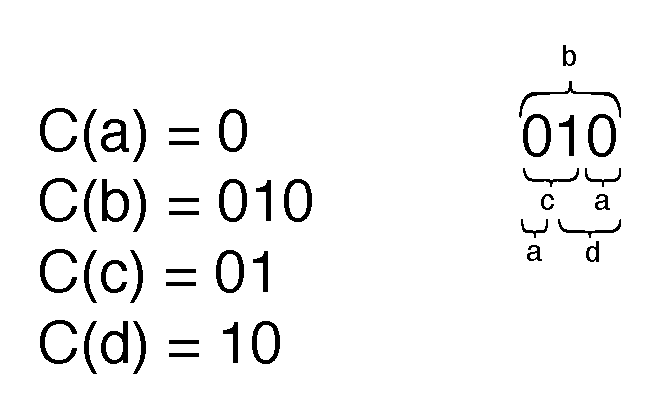
\includegraphics[width=0.4\textwidth]{img/codice3.pdf}
\caption{esempio di codice non singolare ma ambiguo; si pu� notare a destra come la segmentazione presenti delle ambiguit�: la stringa 010 potrebbe infatti essere interpretata come b oppure come c seguito da a, oppure come a seguita da d.}
\label{fig:codice3}
\end{center}
\end{figure}

Abbiamo in sostanza bisogno di un criterio pi� forte per costruire codici non ambigui.
Se C � un codice qualsiasi, la sua estensione k-esima � un codice costruito su stringhe di simboli di X lunghe k:
\[C^k: \X^k \longrightarrow \D^*\]
dove:
\[C^k(x_1... x_k) = C(x_1) C(x_2) ... C(x_k)\]
Consideriamo il codice in figura \ref{fig:codice3}. La sua estensione 2\textordfeminine \ sar� quella rappresentata in tabella \ref{tab:codice4}.

\begin{table}[htbp]
  \begin{center}
   \begin{tabular}{c|c}
	$\X^{2}$ & $ \D^{*}$ \\
       \hline
	$aa$ & $00$ \\ 
	$ab$ & $0010$ \\ 
	$ac$ & $001$ \\ 
        $ad$ & $010$ \\ 
        $ba$ & $0100$ \\ 
        $...$ & $...$ \\ 
    \end{tabular}
     
     \caption{Estensione 2� del codice}
    \label{tab:codice4}
  \end{center}
\end{table}

A partire dall'estensione k-esima possiamo quindi costruire l'estensione, ossia quella che mappa una qualsiasi stringa costruita su simboli di \(\X\) in $D^*$:
\[C^*: \X^* -> \D^*\]
\[C^*(x_1... x_n) = C(x_1) C(x_2) ... C(x_n)\]

\begin{definizione}[Codice U.D.]
Sia \(C: \X \longrightarrow \D^*\) un codice, C si dice \textit{univocamente decodificabile} (UD) se:
\[C^*: \X^* \longrightarrow \D^*\]
(l'\textit{estensione del codice}), � non singolare.
\label{codiceUD}
\end{definizione}

Se un codice � UD, allora il destinatario riuscir� sempre a segmentare i bit in arrivo.
Riprendendo sempre l'esempio precedente, appare chiaro che il codice in figura \ref{fig:codice3}  non � UD Infatti nella sua estensione 2� (tabella \ref{tab:codice4}) compare la sequenza '010', che per� � presenta anche nel codice originale (figura \ref{fig:codice3}).


I codici UD sono sicuramente non ambigui, ma alcuni di essi possono essere inefficienti, come quello rappresentato in figura \ref{fig:0024}: in questo caso il fatto che una parola sia prefisso dell'altra provoca l'introduzione di un ritardo di decodifica. Ci� � dovuto al fatto che � necessario un certo numero di simboli per riuscire a distinguere le due differenti parole. Per ovviare a questo problema introduciamo un'ulteriore classe di codici.

\begin{figure}[htbp]
\begin{center}
	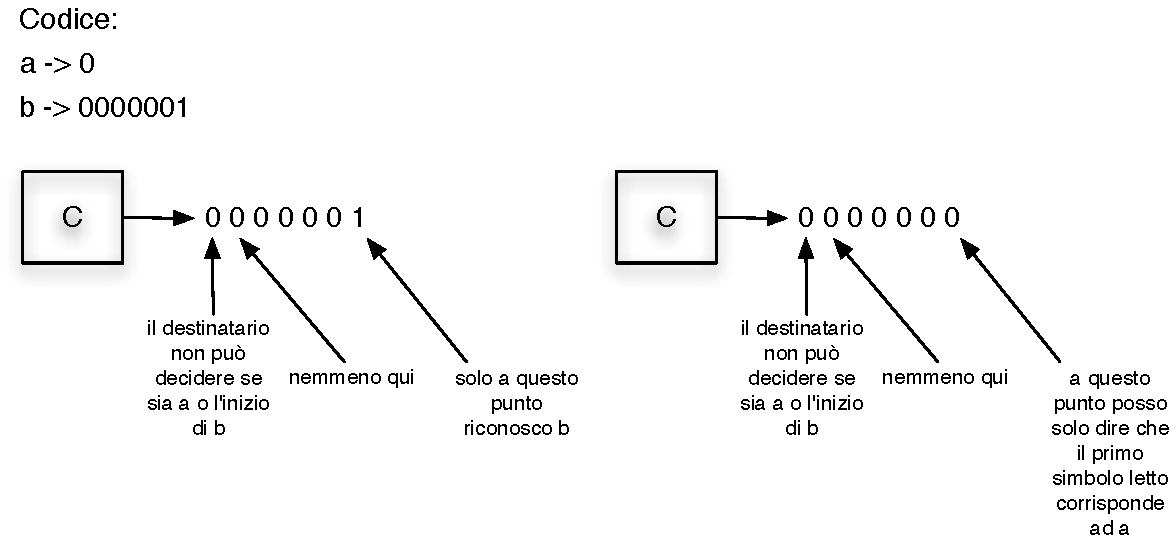
\includegraphics[width=\textwidth]{img/istantaneo.pdf}
\caption{esempio di codice UD poco efficiente (si tratta di un comma code, in quanto l'1 funge da separatore delle stringhe)}
\label{fig:0024}
\end{center}
\end{figure}

\begin{figure}[htbp]
\begin{center}
	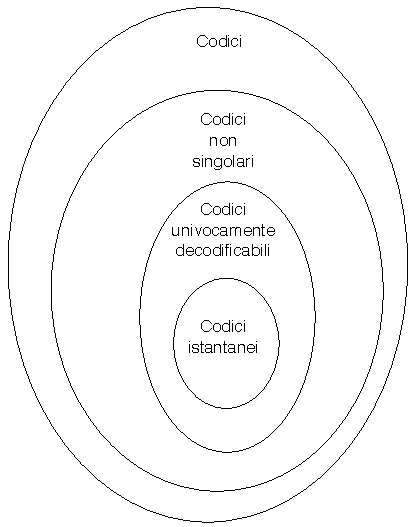
\includegraphics[width=0.5\textwidth]{img/codici.pdf}
\caption{schema riassuntivo dei tipi di codice}
\label{fig:0004}
\end{center}
\end{figure}


\begin{definizione}[codice istantaneo]
Un codice C si dice \textit{istantaneo o a prefisso} se nessuna parola di codice � prefisso di un'altra.
\end{definizione}
Possiamo osservare che un codice istantaneo � sicuramente anche UD (torneremo meglio dopo su questo punto). In sostanza i codici 
istantanei sono un sottoinsieme di quelli UD. Possiamo anche dire che � necessario avere un codice UD (per non avere ambiguit�), tuttavia � preferibile che il codice sia anche istantaneo (pi� efficienza).
In figura \ref{fig:0004} � rappresentato uno schema riassuntivo dei codici visti.





\subsection{Teorema di Sardinas-Patterson}
Non � sempre immediato determinare se un codice sia o meno univocamente decodificabile, in quanto bisognerebbe considerare la sua estensione (che come abbiamo visto � formata da stringhe di lunghezza infinita).
E' necessario quindi un criterio che renda questa operazione pi� semplice. Il teorema di Sardinas-Patterson fornisce un metodo utile.

L'idea base del teorema � la seguente. Supponiamo di avere una stringa binaria di un codice non UD (figura \ref{fig:0018}): ciascuna parola della segmentazione in alto ha il suffisso che � anche prefisso delle corrispondenti parole nella segmentazione in basso; il problema si verifica quando il suffisso di una parola della segmentazione in alto coincide con una parola intera della segmentazione alternativa, perch� questo pu� dar luogo a una doppia interpretazione. Se invece le segmentazioni si intersecano sempre, senza mai che un suffisso e una parola coincidano, allora il codice � UD.

\begin{figure}[htbp]
\begin{center}
	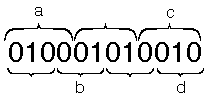
\includegraphics[width=0.4\textwidth]{img/ud.pdf}
\caption{a ha il suffisso che � prefisso di b; c ha il suffisso che coincide con l'intera parola d}
\label{fig:0018}
\end{center}
\end{figure}

\begin{teorema}[di Sardinas-Patterson]
Dato un codice \(C: X -> \D^*\), e posti:
\[S_0 = C(X_0) = \{C(x) \in \D^* | x \in X_0\}\]
\[\forall \ n \geq 1 : S_n = \{w \in D^* | \exists \ a \in S_0, \exists \ b \in S_{n-1} \ t.c. \  a = bw \lor b = aw\}\]
(ossia l'insieme dei suffissi), allora condizione necessaria e sufficiente affinch� C sia univocamente decodificabile �:
\[\forall \ n \geq 1 : S_0 \cap S_n = \varnothing\]
ossia nessuno dei suffissi generati dovr� corrispondere con una parola di codice.
\end{teorema}

Perch� un codice sia UD bisogna verificare la condizione per qualsiasi valore di n, quindi dovremmo iterare il procedimento fino a trovare il primo n per cui la condizione � violata. Ma questo potrebbe non accadere mai (e questo � ovvio nel caso in cui si stia analizzando un codice UD), e quindi l'algoritmo itererebbe all'infinito. Tuttavia l'insieme dei suffissi generabili � finito, quindi il processo prima o poi comincer� a generare insiemi gi� generati: in tal caso la procedura termina (e il codice � UD). Pu� verificarsi anche il caso in cui a un certo punto si genera l'insieme vuoto: anche qui la procedura termina e il codice � UD (da ora in poi saranno tutti insiemi vuoti).

\bigskip
\noindent
\textbf{Esempio}

\noindent
Verifichiamo se il codice ($S_0$ in figura \ref{fig:0019}) � UD: il procedimento � rappresentato sempre in figura \ref{fig:0019}:
\begin{enumerate}
\item \(S_0\) � il codice di partenza;
\item per costruire \(S_1\) vado a vedere se qualche parola di \(S_0\) � prefisso di qualcun'altra nello stesso insieme; se ne trovo vado a prendere il suffisso e lo metto in \(S_1\): a � prefisso di ab e abb, quindi inseriamo in \(S_1\) i corrispondenti suffissi d e bb;
\item controllo se gli elementi di \(S_1\) ci sia una parola di codice, cosa non vera, per cui proseguo;
\item per costruire \(S_2\) vado a vedere se qualche parola di \(S_1\) � prefisso di qualche parola di \(S_0\) o se qualche parola di \(S_0\) � prefisso di qualche parola di \(S_1\); se ne trovo vado a prendere il suffisso e lo metto in \(S_1\): d � prefisso di deb, mentre bb di bbcde, quindi inseriamo in \(S_2\) i corrispondenti suffissi eb e cde;
\item controllo se gli elementi di \(S_2\) ci sia una parola di codice, cosa non vera, per cui proseguo;
\item e cos� via...
\item arrivato ad  \(S_5\) scopro che ad � una parola di codice, quindi possiamo concludere che il codice non � UD.
\end{enumerate}
Altri due esempi di applicazione del teorema di Sardinas-Patterson sono rappresentati nelle figure \ref{fig:0020} e \ref{fig:0021}.

\begin{figure}[htp]
\begin{center}
	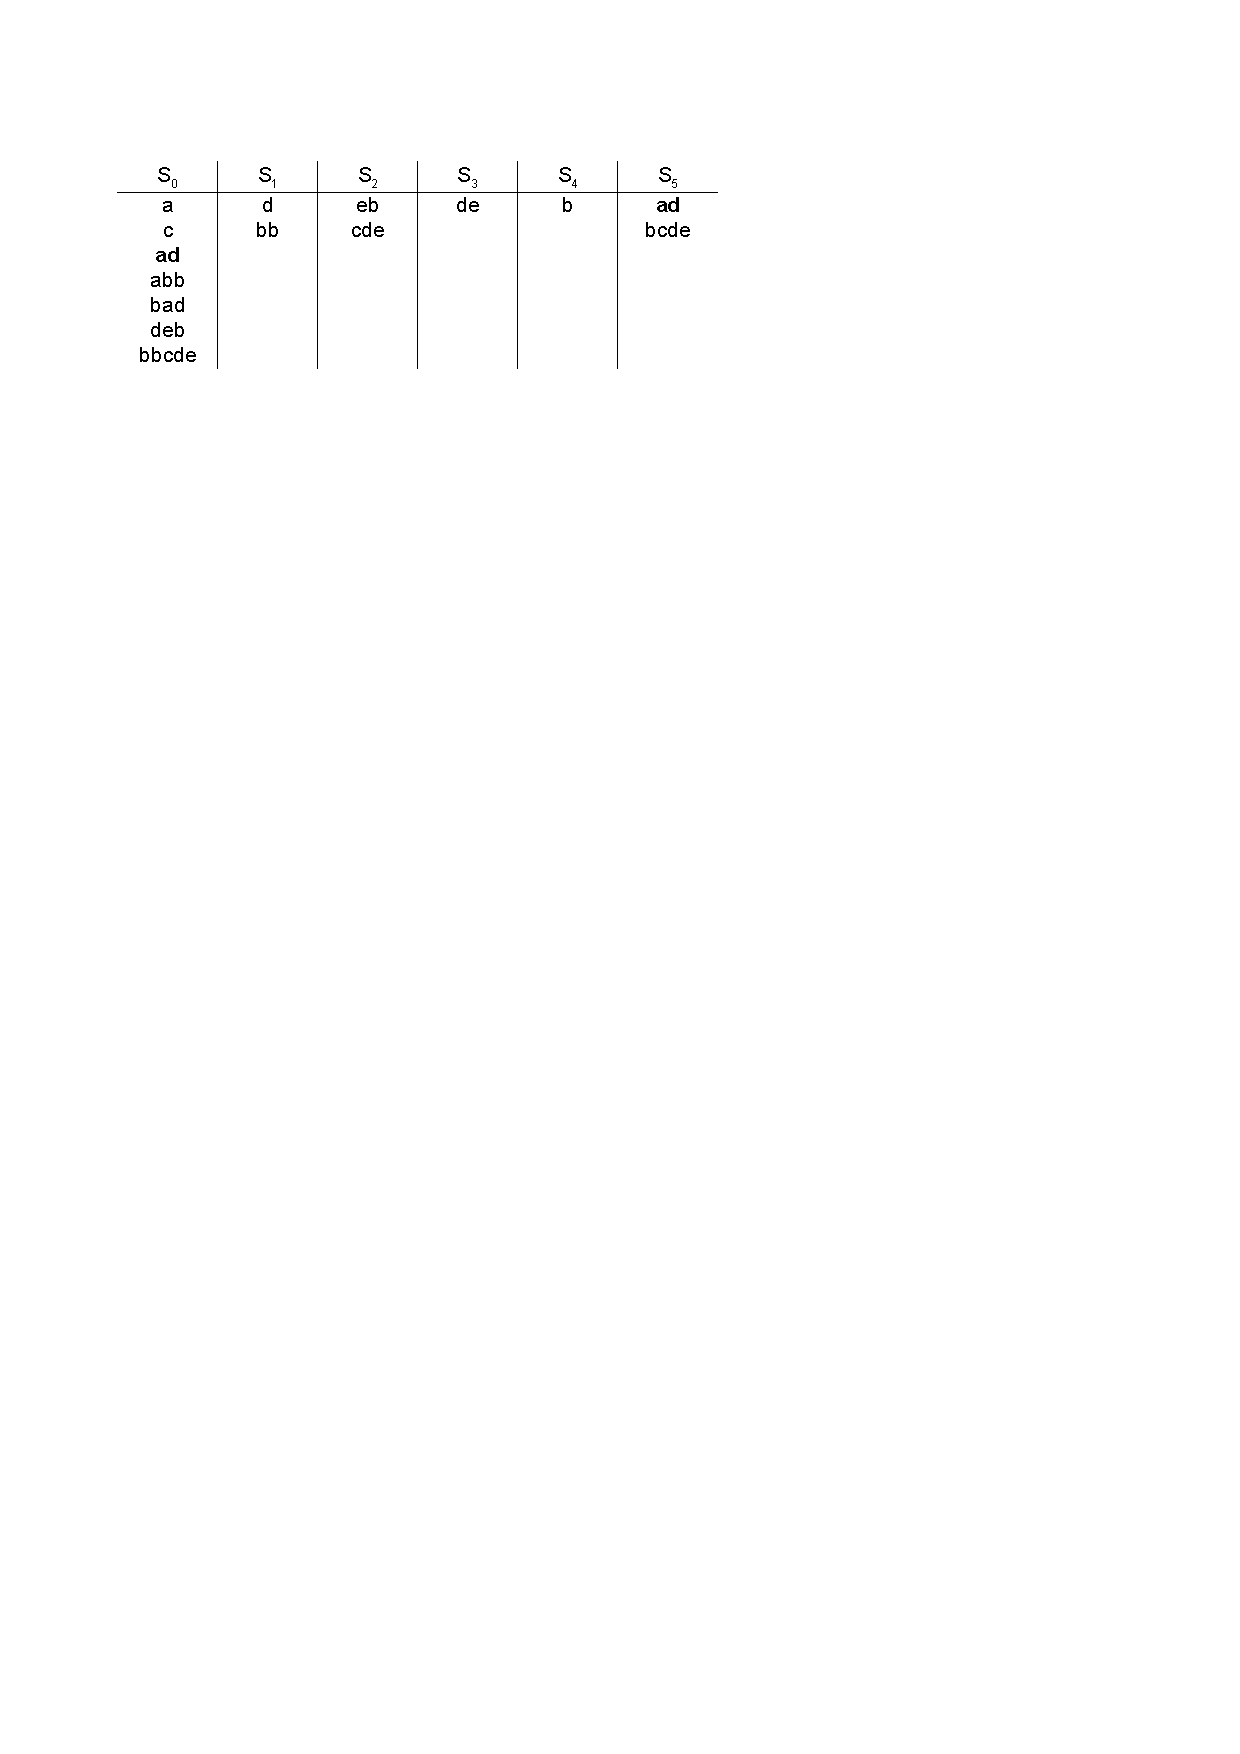
\includegraphics[width=\textwidth]{img/patt1.pdf}
	
\includegraphics[width=0.2\textwidth]{img/patt1b.pdf}
\caption{procedimento basato sul teorema di Sardinas-Patterson; il codice non � UD. In basso un esempio di ambiguit�}
\label{fig:0019}
\end{center}
\end{figure}

\begin{figure}[htp]
\begin{center}
	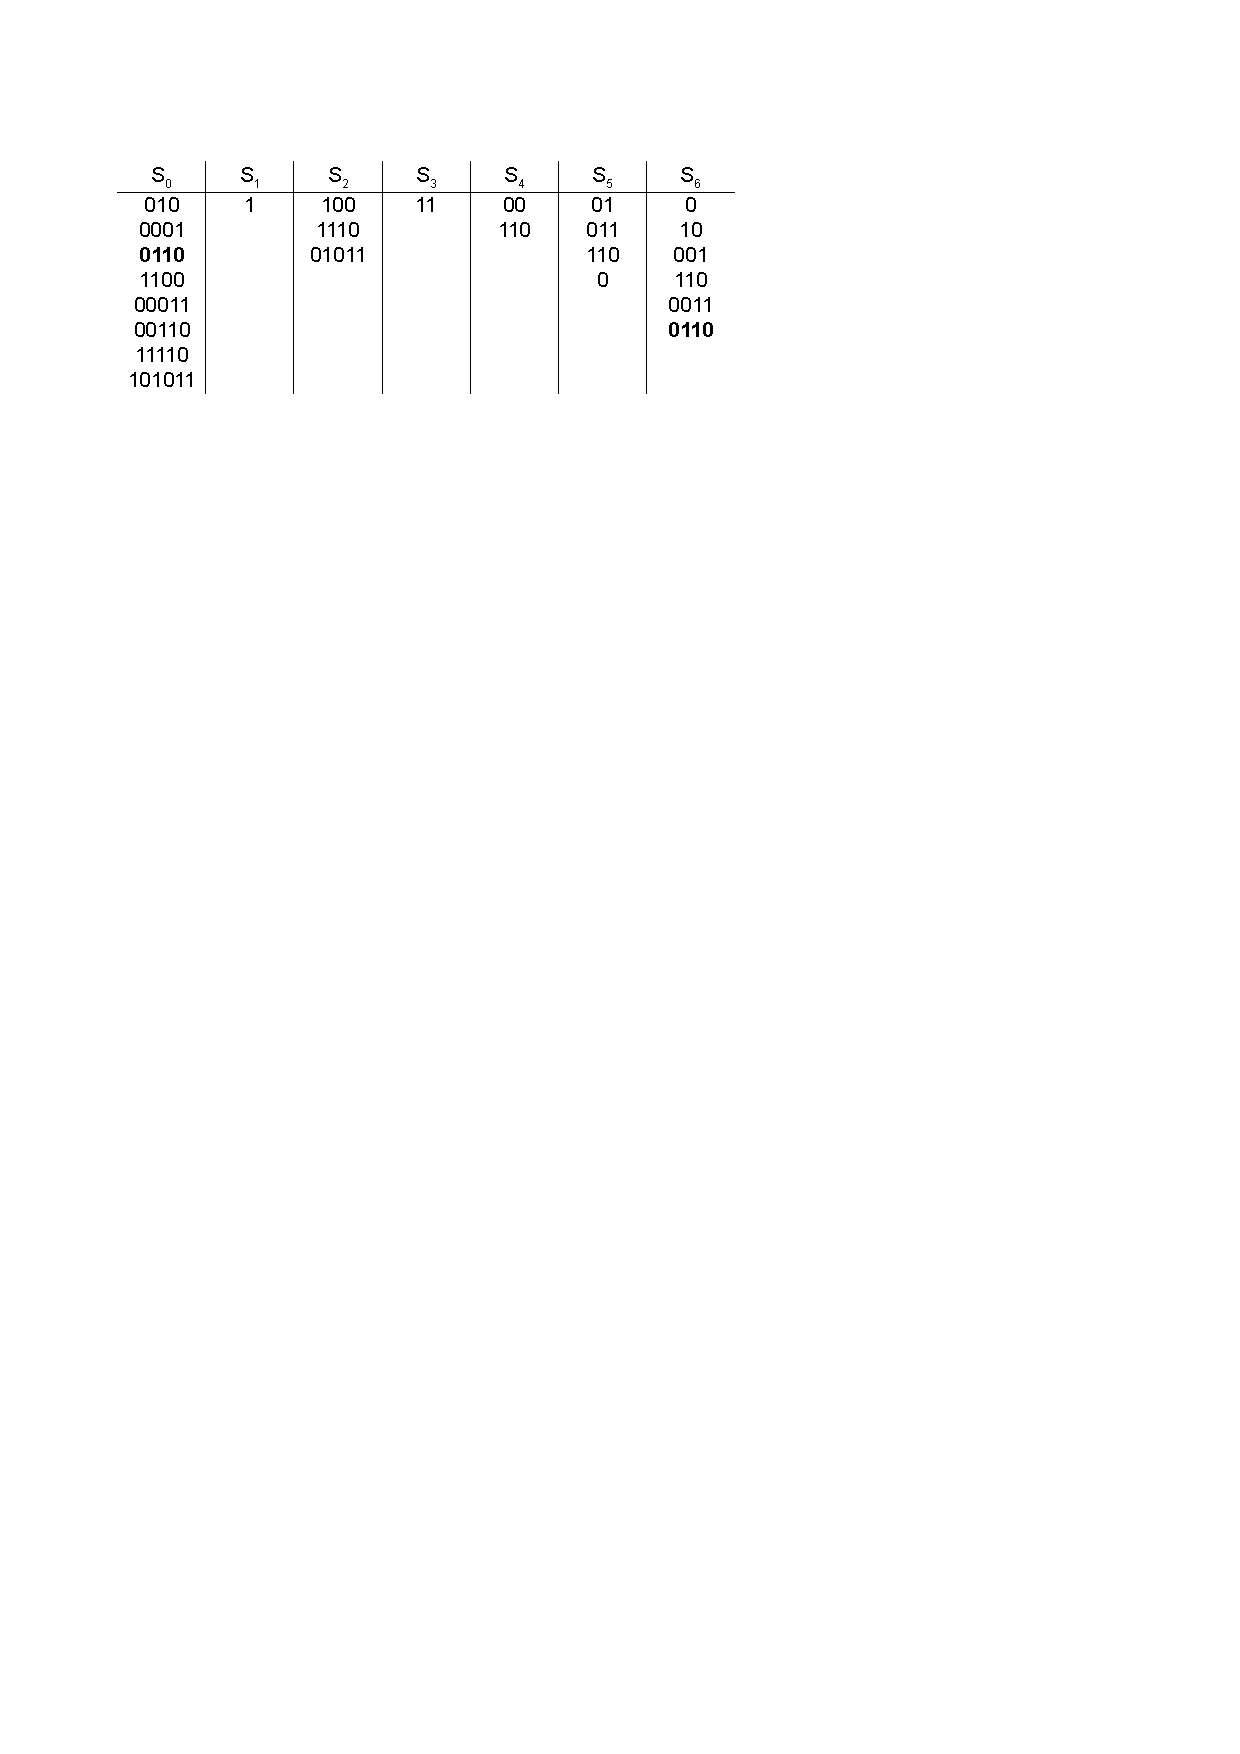
\includegraphics[width=\textwidth]{img/patt2.pdf}
\caption{procedimento basato sul teorema di Sardinas-Patterson, il codice non � UD}
\label{fig:0020}
\end{center}
\end{figure}

\begin{figure}[htp]
\begin{center}
	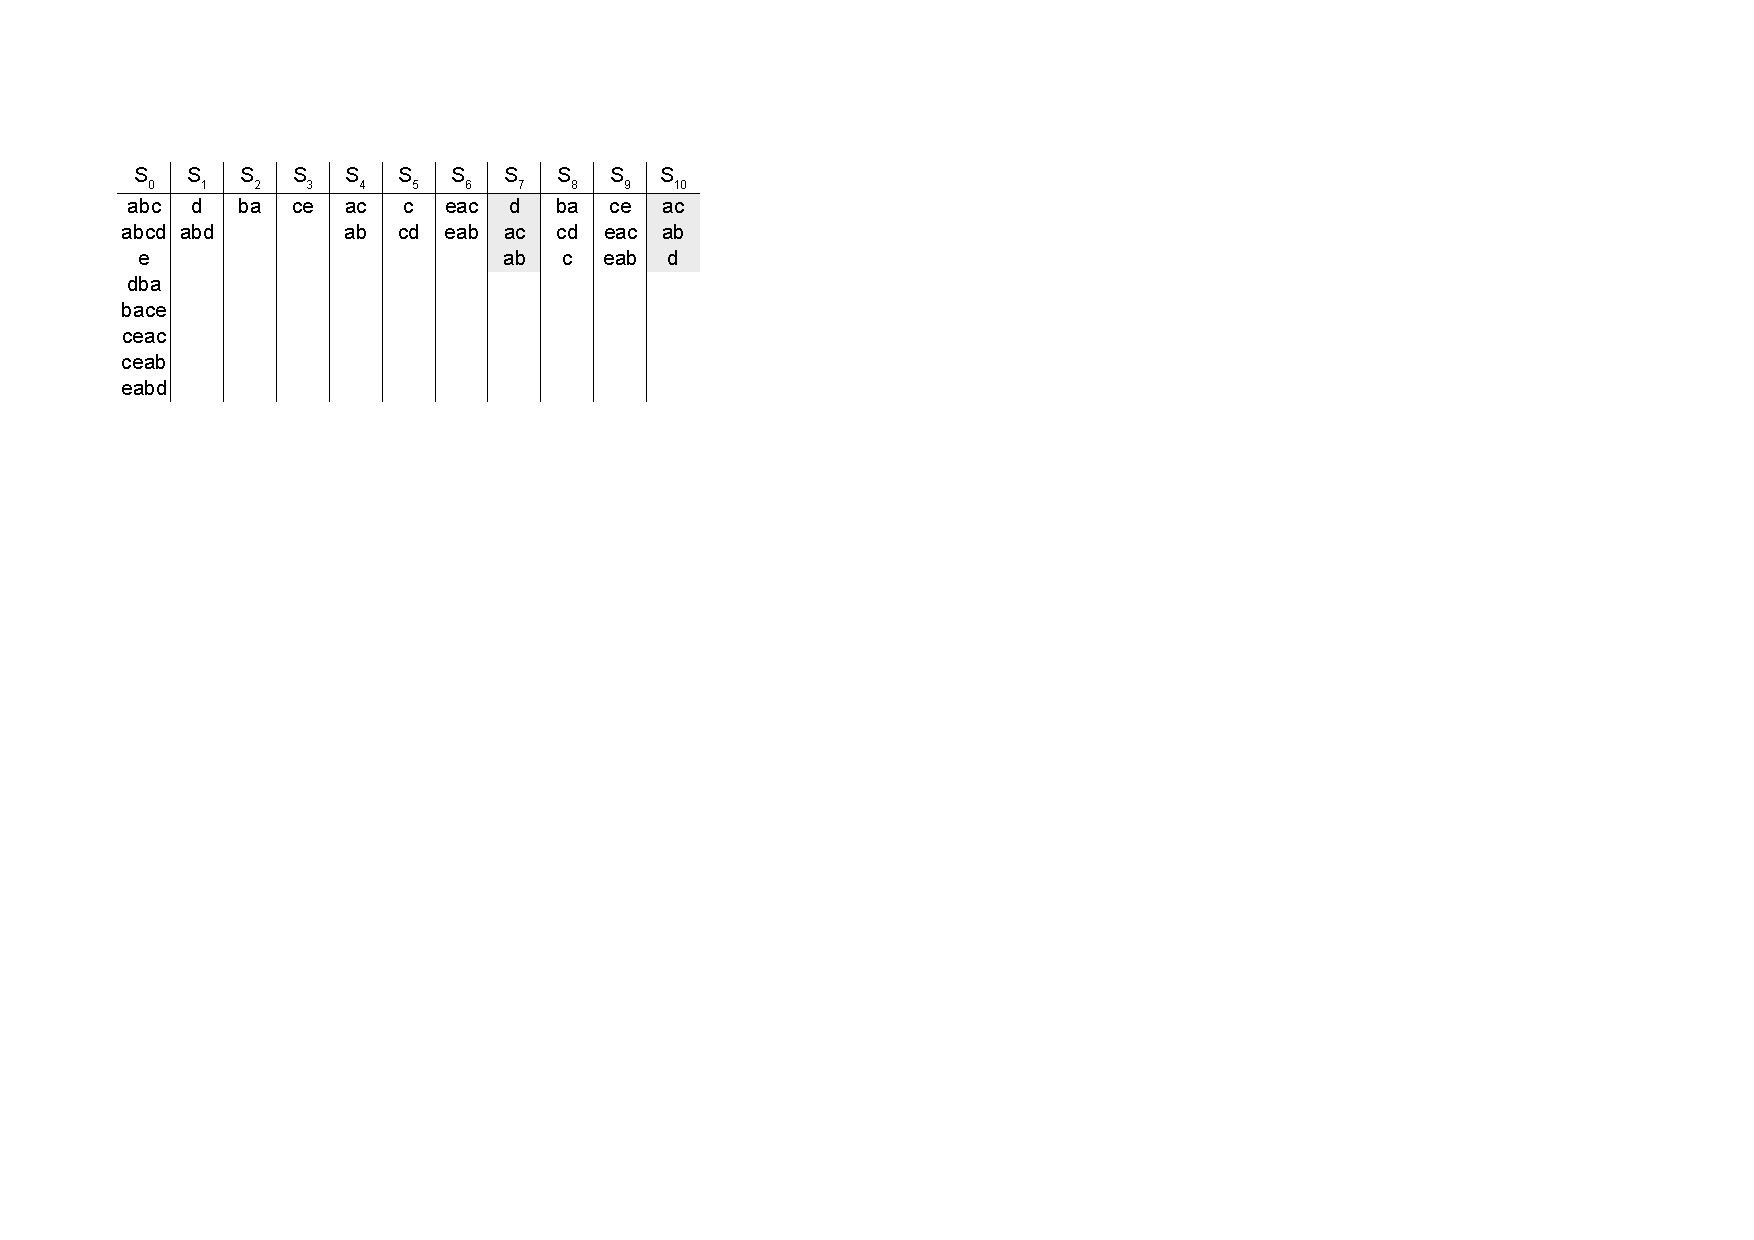
\includegraphics[width=0.9\textwidth]{img/patt3.pdf}
\caption{procedimento basato sul teorema di Sardinas-Patterson, il codice � UD}
\label{fig:0021}
\end{center}
\end{figure}

\newpage

\section{Costruzione di codici}
Sono stati visti vari tipi di codici. Inoltre abbiamo evidenziato come le classi di maggior interesse siano quelle dei codici istantanei 
ed univocamente decodificabili. Vediamo ora quali condizioni devono valere, affinch� sia possibile costruirli.

\subsection{Disuguaglianza di Kraft}
La Disuguaglianza di Kraft, fornisce un vincolo importante per la costruzione di codici istantanei.
Infatti, affinch� sia possibile costruire un codice istantaneo, la lunghezza delle parole di codice deve rispettare un vincolo.
\`E importante notare che il teorema esprime la possibilit� di costruire un codice istantaneo. In altre parole, se il teorema vale allora con determinate lunghezze di parole di codice si pu� un costruire un codice istantaneo. Tuttavia non tutti i codici con quelle determinate lunghezze sono istantanei!

\begin{teorema}[Disuguaglianza di Kraft]
\label{kraft}
Condizione necessaria e sufficiente \textbf{affinch� sia possibile} costruire un codice istantaneo D-ario (ossia un codice costruito su un alfabeto di D simboli) con lunghezza di parola \(l_1, l_2 ... l_n\) �:
\[\sum_{i = 1}^n D^{-l_i} \leq 1\]
\begin{proof}
A partire da un codice D-ario, possiamo costruire il corrispondente \textbf{albero D-ario di codifica} (figura \ref{fig:albero}).
L'albero ha profondit� pari alla lunghezza della parola pi� grande e ciascun vertice (o ciascun cammino) rappresenter� una sequenza 
di simboli (la cui lunghezza � al massimo la lunghezza della parola pi� lunga).
Nell'albero si evidenziano i vertici, i cui cammini dalla radice corrispondono ad una parola di codice.
In questo modo si costruisce una corrispondenza biunivoca tra il codice e l'albero.
E' facile osservare che un codice � istantaneo se e solo se nel corrispondente albero di codifica non esistono due vertici evidenziati che appartengono uno al sottoalbero dell'altro. In altre parole, percorrendo il cammino dalla radice ad un vertice evidenziato, non devo incontrare altri vertici evidenziati.

\begin{figure}[htbp]
\begin{center}
	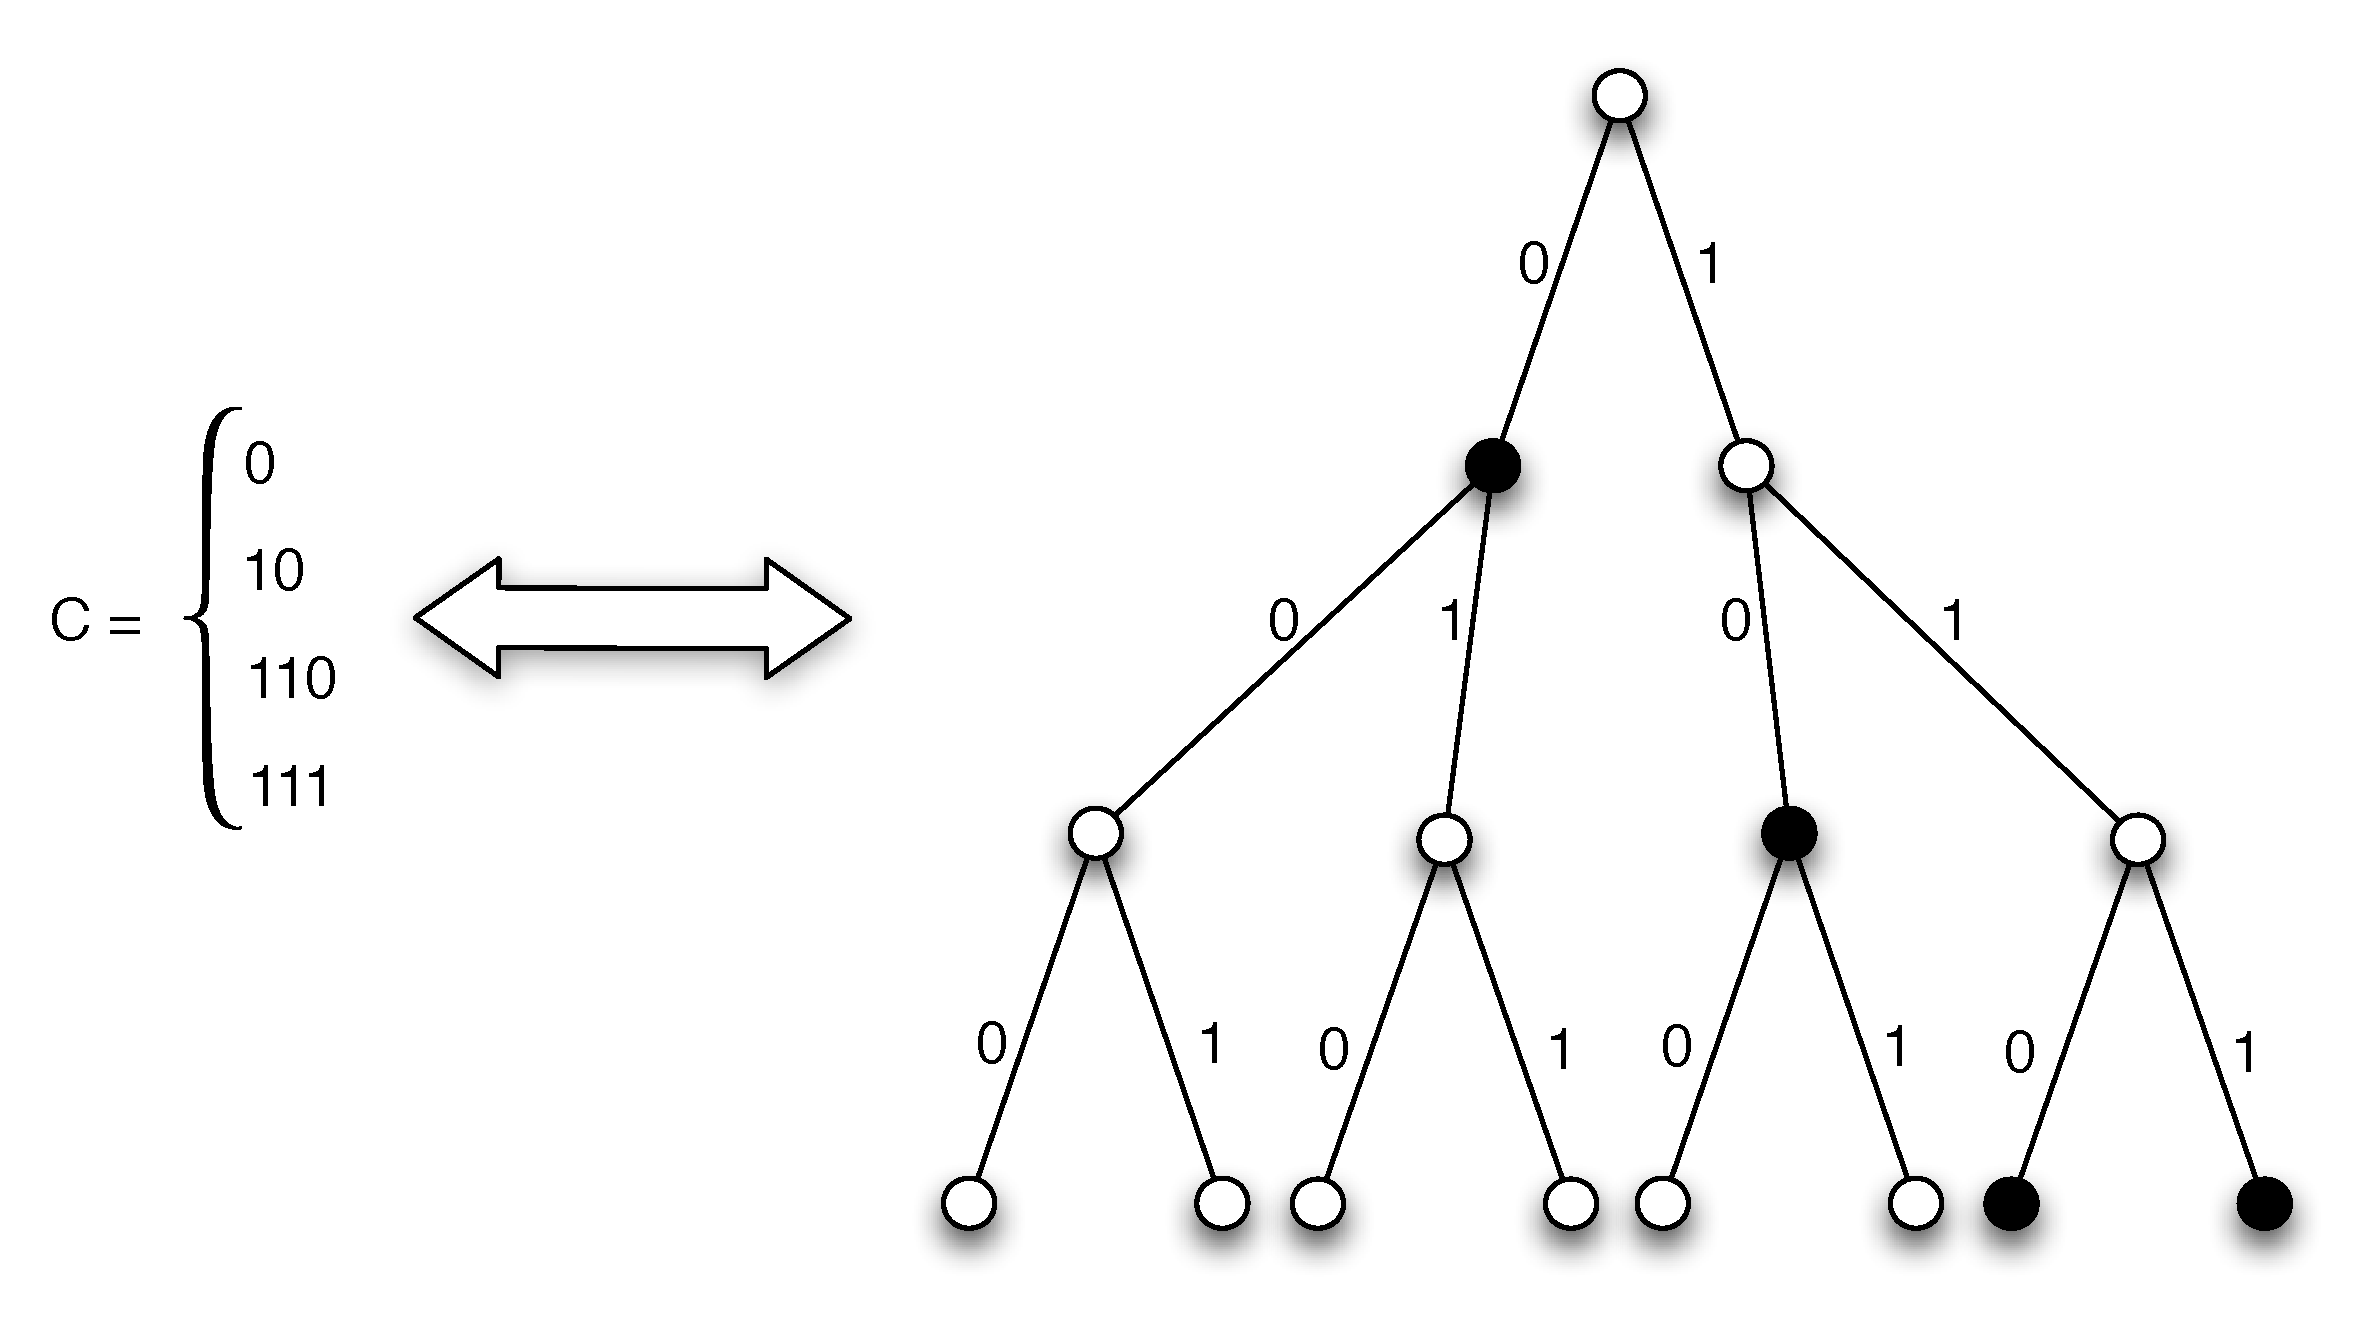
\includegraphics[width=\textwidth]{img/kraft.pdf}
\caption{Esempio di codice e corrispondente albero binario}
\label{fig:albero}
\end{center}
\end{figure}

Dobbiamo ora dimostrare le due implicazioni:
\begin{description}
\item[\(\Longrightarrow\)]: supponiamo che C sia un codice istantaneo D-ario e assumiamo che le lunghezze delle parole di codice siano ordinate in maniera crescente:
\[l_1 \leq l_2 ... \leq l_n\]
Dobbiamo  quindi dimostrare che vale la disuguaglianza del teorema.
Poich� il codice � istantaneo, nessuna parola di codice � prefisso di qualcun'altra. Nella rappresentazione dell'albero, quindi, preso il sottoalbero che fa capo ad una parola di codice, nessun altro vertice corrispondente ad altre parole di codice � contenuto in tale sottoalbero. Di conseguenza i sottoalberi radicati nei vertici delle varie parole di codice non si intersecano.

Siamo ora interessati al numero di foglie di ogni sottoalbero (che fa capo ad una parola di codice). E' facile osservare che un albero 
D-ario ha \(D^{h}\) foglie, con h profondit� dell'albero. Ma in questo caso la profondit� � pari alla lunghezza della parola di codice pi� lunga, l'albero avr� dunque \(D^{l_n}\) foglie. Poich� i vari sottoalberi non si intersecano, deve essere:
\[
 \mid I_1 \mid + \mid I_2 \mid + ... + \mid I_n \mid \le D^{l_n}
\]

\begin{figure}[htbp]
\begin{center}
	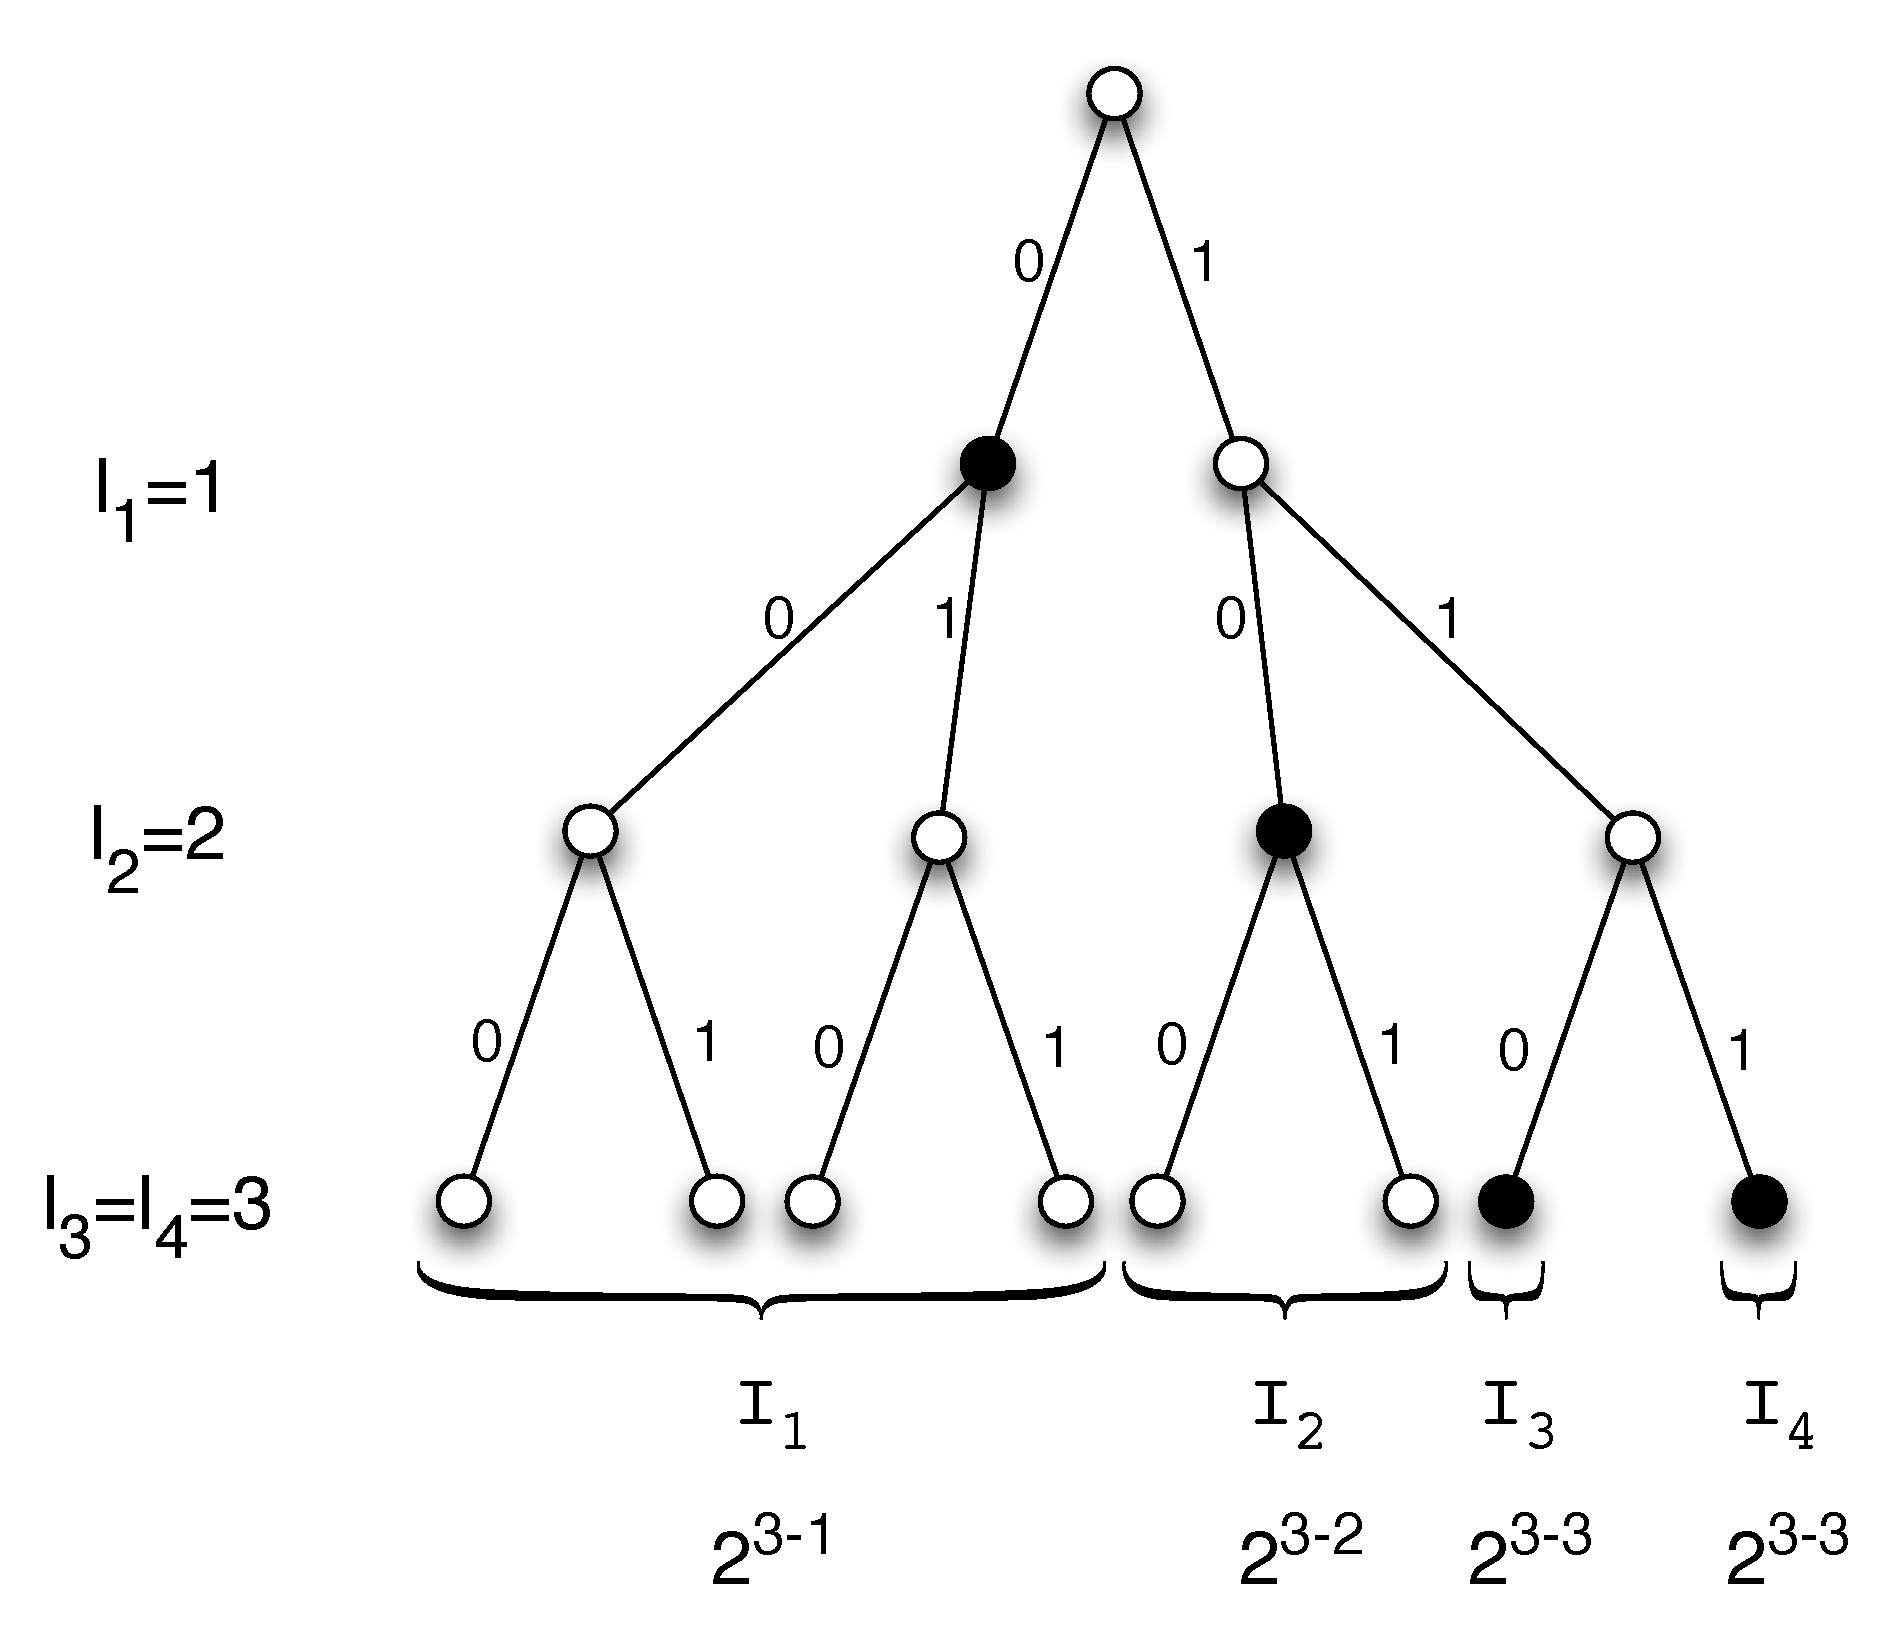
\includegraphics[width=0.7\textwidth]{img/kraft2.pdf}
\caption{Esempio di albero binario associato ad un codice, con varie quantit� evidenziate}
\label{fig:albero2}
\end{center}
\end{figure}

Dove con $\mid I_i \mid$ abbiamo indicato il numero di foglie del sottoalbero corrispondente alla parola di codice i.
Per ricavare tale numero, � possibile utilizzare ancora la formula \(D^{h}\). Questa volta per� l'altezza � quella del sottoalbero 
che fa capo alla parola i. Per come � costruito l'albero, si ricava che tale altezza vale $l_n-l_i$ (figura \ref{fig:albero2}).

Risulta quindi:
\[ D^{l_n- l_1} + D^{l_n- l_2} + ... D^{l_n- l_n} \leq D^{l_n}\]

Da cui:
\[\begin{split}
 &\sum_{i = 1}^n D^{l_n-l_i} \leq D^{ln} \\
 \Rightarrow &\sum_{i = 1}^n D^{l_n} \cdot D^{-l_i} \leq D^{l_n} \\
 \Rightarrow &D^{l_n} \sum_{i = 1}^n D^{-l_i} \leq D^{l_n} \\
 \Rightarrow &\sum_{i = 1}^n D^{-l_i} \leq 1
 \end{split}
\]

\item[\(\Longleftarrow\)]: supponiamo che valga:
\[\sum_{i = 1}^n D^{-l_i} \leq 1\]
con \(l_1 \leq l_2 ... \leq l_n\) e dimostriamo come sia possibile costruire un codice istantaneo con tali lunghezze.
A tal scopo, costruiamo un codice con il seguente algoritmo:
\begin{enumerate}
\item Presa la prima foglia da sinistra non compresa in un sottoalbero (tra quelli evidenziati nel punto 2), risali fino al livello \(l_i\)
\item Aggiungi la sequenza associata ad \(l_i\) all'insieme delle parole di codice (ed evidenzia il suo sottoalbero)
\item Se non hai raccolto n parole di codice, torna ad 1
\end{enumerate}
Il codice cos� ottenuto � istantaneo, poich� non ci sono intersezioni fra i sottoalberi corrispondenti alle parole di codice. 
Un esempio dell'applicazione dell'algoritmo � riportato in figura \ref{fig:albero3}.

\begin{figure}[htbp]
\begin{center}
	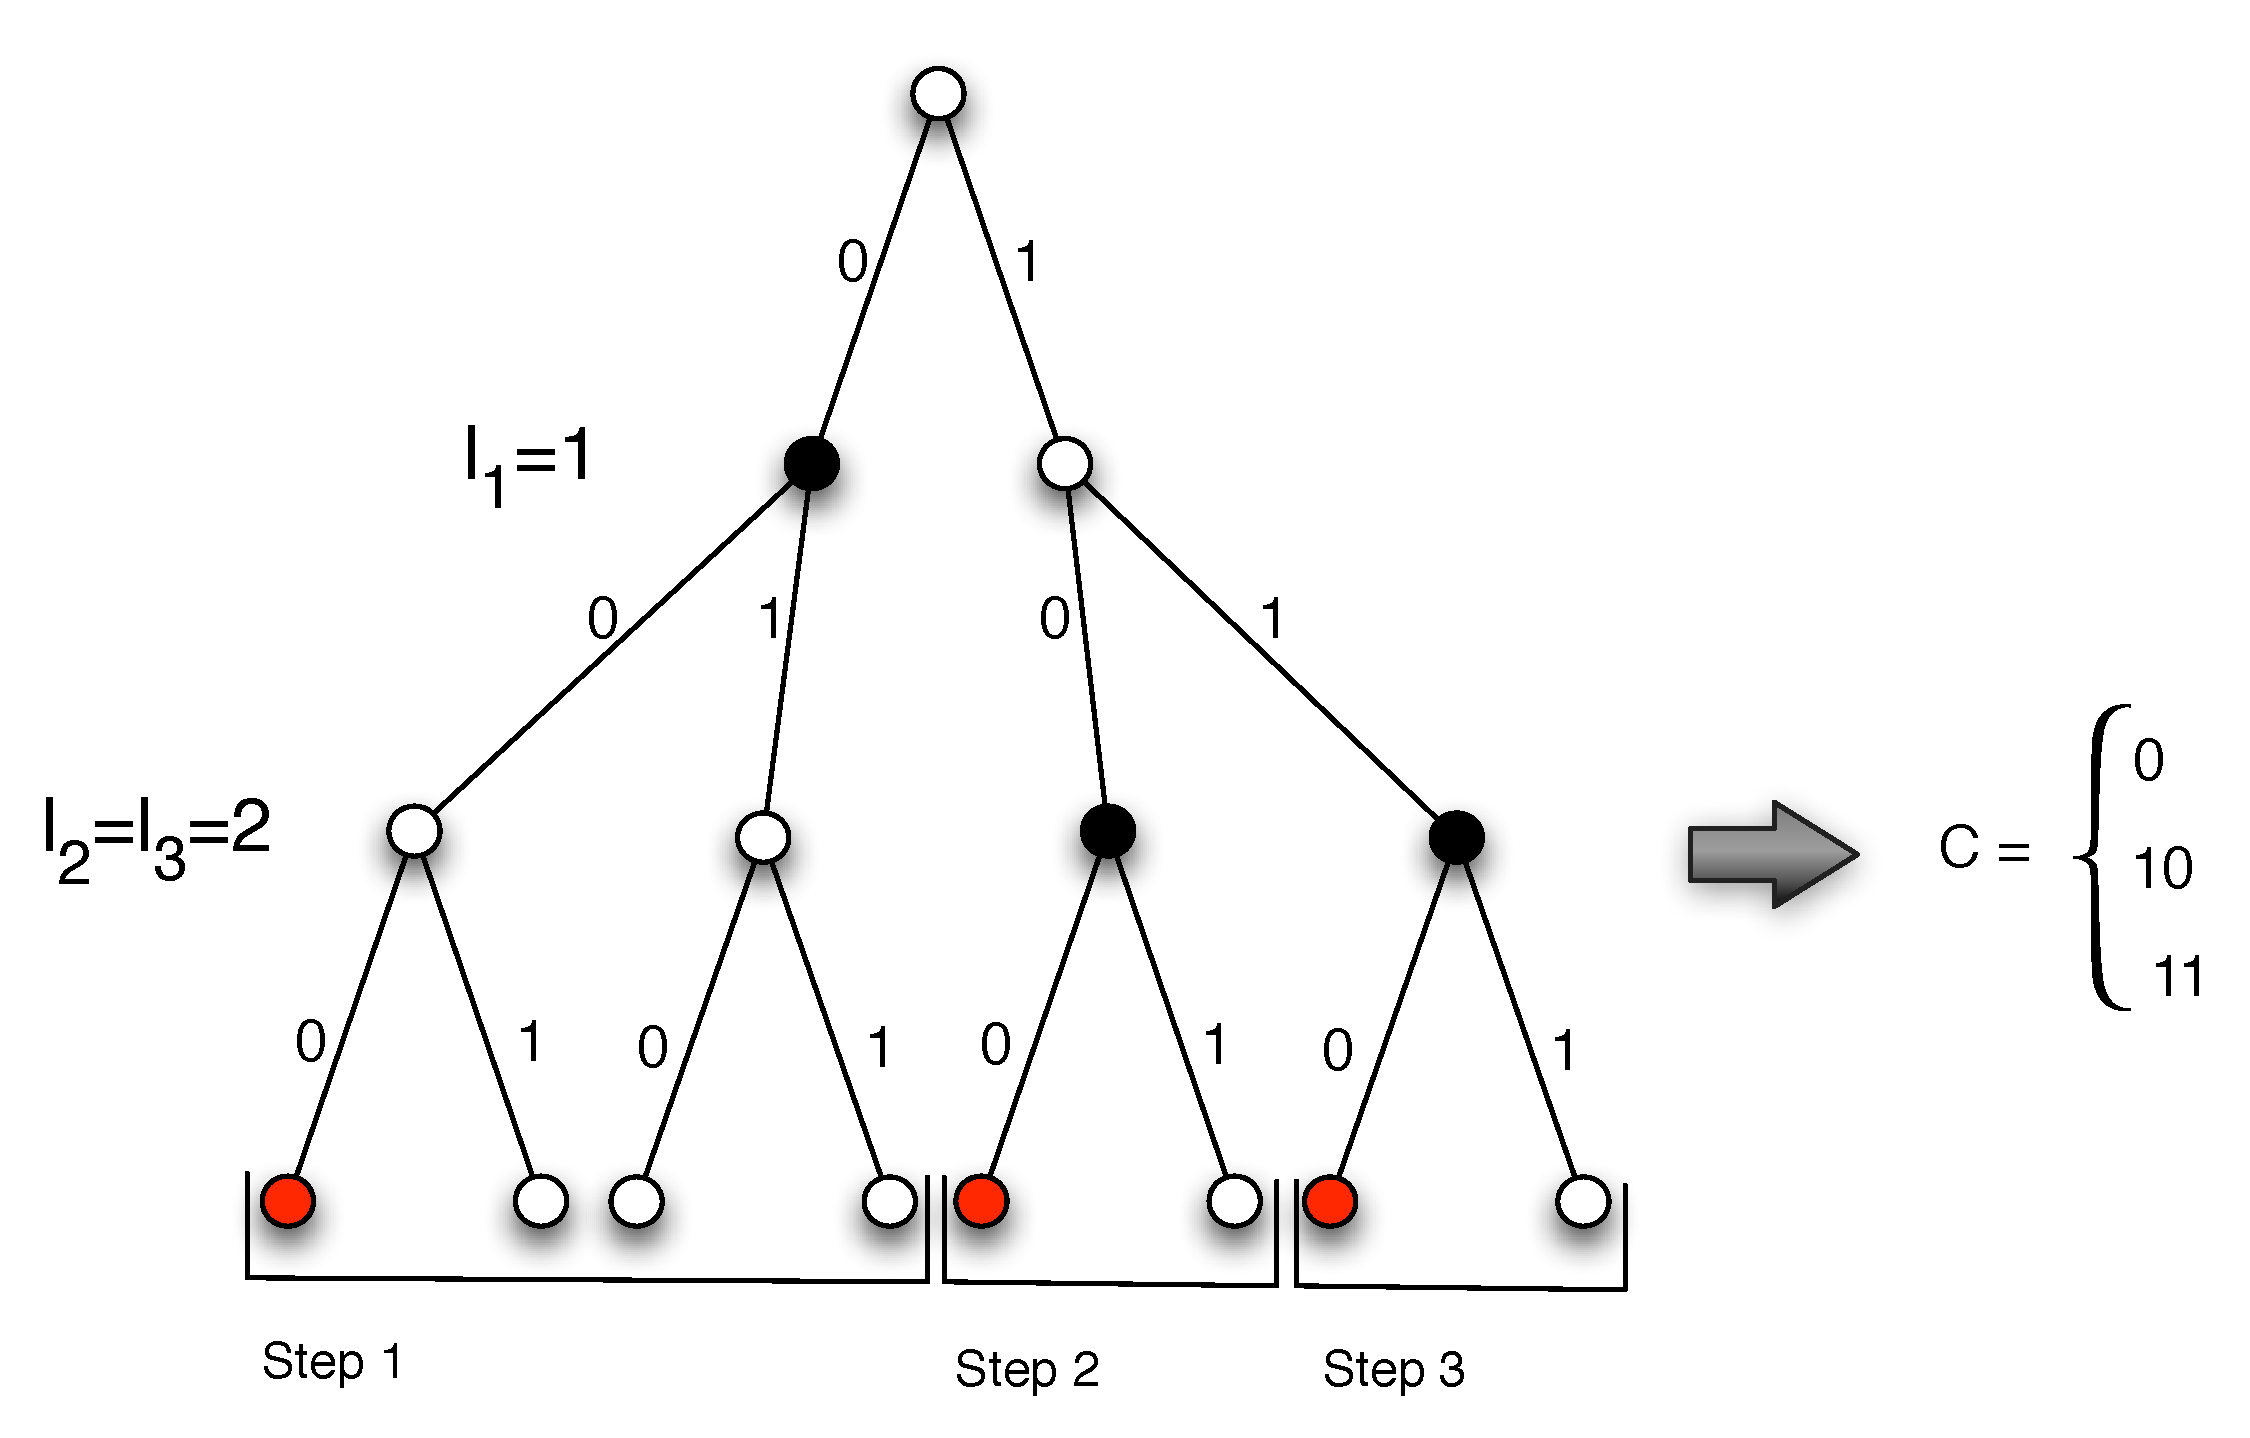
\includegraphics[width=0.9\textwidth]{img/kraft3.pdf}
\caption{Esempio dell'algoritmo per generare il codice istantaneo}
\label{fig:albero3}
\end{center}
\end{figure}

Prima di poter concludere la dimostrazione, � fondamentale risolvere una questione importante. Dobbiamo infatti essere sicuri che ci siano sempre foglie disponibili da cui scegliere ad ogni iterazione dell'algoritmo.
Ovvero l'insieme delle foglie non disponibili (perch� facente parti di un sottoalbero) deve essere strettamente 
minore delle foglie totali.
Il numero totale di foglie, come visto prima, � $D^{ln}$. Il numero di foglie non disponibili al passo 0 � 0 (sono tutte disponibili), al passo 1 � $D^{ln-l1}$, al passo 2 � $D^{ln-l1}+D^{ln-l2}$, al passo j � $\sum_{i = 1}^j D^{ln-l_j}$.
Deve quindi essere:
\[
 \forall k=1..n-1 \ : \ \sum_{i = 1}^k D^{ln-l_i} < D^{ln} 
\]

In maniera analoga all'implicazione precedente abbiamo che:
\[
 \begin{split}
  & \sum_{i = 1}^n D^{-l_i} \leq 1 \\
  \Rightarrow & D^{ln} \sum_{i = 1}^n D^{-l_i} \leq D^{ln} \\
  \Rightarrow & \sum_{i = 1}^n D^{ln-l_i} \leq D^{ln}  
 \end{split}
\]

Poich� D � positivo:
\[
\forall i=1..n \ : \ D^{ln-l_i} > 0
\]
Da cui:
\[
  D^{ln-l_1} < D^{ln-l_1} + D^{ln-l_2} < ... < \sum_{i = 1}^{n-1} D^{ln-l_i}  < \sum_{i = 1}^n D^{ln-l_i} \leq D^{ln}  
\]

Quindi esiste sempre una foglia disponibile ad ogni passo dell'algoritmo.
\end{description}
\end{proof}
\end{teorema}

\subsection{Disuguaglianza di McMillan}
Prima di presentare la disuguaglianza, forniamo un lemma utili per la dimostrazione:

\begin{lemma}
 \[
  \forall \alpha > 0 \ : \ \lim_{n \to \infty} \sqrt[n]{\alpha}=1
 \]
\label{lemmaMillan}
\end{lemma}


\begin{teorema}[Disuguaglianza di McMillan]
Condizione necessaria e sufficiente \textbf{affinch� sia possibile} costruire un codice univocamente decodificabile D-ario (ossia un codice costruito su un alfabeto di D simboli) con lunghezza di parola \(l_1, l_2 ... l_n\) �:
\[\sum_{i = 1}^n D^{-l_i} \leq 1\]
\label{macmillan} 

\begin{proof}
Dobbiamo ora dimostrare le due implicazioni:
\begin{description}
\item[\(\Longleftarrow\)]: 
Banale. La disuguaglianza � identica a quella di Kraft. Pertanto possiamo costruire un codice istantaneo, che come abbiamo gi� visto � anche UD.
\item[\(\Longrightarrow\)]:
Supponiamo di aver costruito un codice $C: \ \X \to D^*$ univocamente decodificabile.
Indicando con l(x) la lunghezza della parola di codice associata ad $x \in X$, dobbiamo dimostrare che:

\[\sum_{x \in \X} D^{-l(x)} \leq 1\]

Consideriamo l'estensione k-esima ($k>1$) di C, $C^k : \X^k \to D^*$.
Poich� C � UD, la sua estensione k-esima sar� non singolare (per definizione di codice UD [\ref{codiceUD}]).
Consideriamo poi la potenza k-esima della parte sinistra della disuguaglianza:
\[\begin{split}
&\left[ \sum_{x \in \X} D^{-l(x)} \right]^k \\
 =& \sum_{a_1 \in \X} D^{-l(a_1)} \sum_{a_2 \in \X} D^{-l(a_2)} ... \sum_{a_k \in \X} D^{-l(a_k)} \\
 =&\sum_{a_1 \in \X} \sum_{a_2 \in \X} ... \sum_{a_k \in \X} \left [ D^{-l(a_1)} D^{-l(a_2)} ... \ D^{-l(a_k)} \right ] \\
 =&\sum_{\bar{a} \in \X^k} D^{-l(\bar{a})}
\end{split}
\]

Dove $\bar{a}=(a_1,a_2,..a_k)$ e $l(\bar{a})=l(a_1)+l(a_2)+...+l(a_k)$

Definiamo ora la sequenza pi� lunga in X:
\[
 l_{max} = max \{l(x) | x \in \X \}
\]
Definiamo poi l'insieme delle sequenze in $X^k$ di lunghezza m:
\[
 A_m^k=\{ \bar{x} \in X^k \mid l(\bar{x})=m \}
\]
E il numero di tali sequenze:
\[
 {\alpha}_m^k=| A_m^k |
\]
Possiamo allora riscrivere la sommatoria precedente, ordinandola in base alle lunghezze delle parole:
\[
 \sum_{\bar{a} \in \X^k} D^{-l(\bar{a})}=\sum_{m=1}^{k l_{max}} {\alpha}_m^k D^{-m}
\]

Poich� $C^k$ � non singolare deve essere:
\[\alpha_m^k \leq D^m\] 
Infatti $D^m$ � il numero di sequenze lunghe m che possono costruire con D simboli. Affinch� $\alpha_m^k$ sia pi� grande, 
dovrebbero per forza esserci due sequenze uguali (cosa impossibile, perch� appunto $C^k$ � non singolare).
Pertanto:
\[\begin{split}
 & \sum_{m=1}^{k l_{max}} {\alpha}_m^k D^{-m} 
 \le \sum_{m=1}^{k l_{max}} D^m D^{-m} \\
 =&\sum_{m=1}^{k l_{max}} 1 
 =k l_{max}
  \end{split}
\]

Riassumendo:
\[
 \forall k>1 \ : \ \left[ \sum_{x \in \X} D^{-l(x)} \right]^k \le k l_{max}
\]

Facendo ora la radice k-esima:
\[
\forall k>1 \ : \ \sum_{x \in \X} D^{-l(x)} \le \sqrt[k]{k} \sqrt[k]{l_{max}}
\]
Poich� la disuguaglianza vale per ogni k, varr� anche per k che tende ad infinito.
Possiamo allora utilizzare il lemma \ref{lemmaMillan} per ottenere:
\[
 \sum_{x \in \X} D^{-l(x)} \le 1
\]

che conclude la dimostrazione.

\end{description}
\end{proof}
\end{teorema}


\section{Codici}
\subsection{Limite alla lunghezza di un codice}
Abbiamo gi� introdotto il concetto di efficienza di un codice. In particolare, abbiamo evidenziato come un codice efficiente debba 
avere una lunghezza (media) piccola. Tuttavia, questa osservazione ci consente solo di confrontare tra loro due codici, ma non riusciamo 
a determinare se una data lunghezza � ``buona'' o meno.
Il seguente teorema fornisce un limite inferiore alla lunghezza di codice. E' importante notare che anche un codice ottimale pu� 
(e come si vedr� � quello che accade) non riuscire sempre a raggiungere tale limite.

\begin{teorema} Sia C un codice D-ario univocamente decodificabile, per la variabile aleatoria 
$X \sim p(X_i)=p_i$. Allora:
\begin{itemize}
\item[(i)]
$
 L(C) \ge H_D(X) = \frac{H(X)}{log(D)}
$
\item[(ii)]
$
 L(C) = H_D(X) \iff \forall x_i \in X: -log_D(p(x_i))=l(x_i)
$
\end{itemize}
\label{limitelcodice}
\begin{proof}
\mbox{}

\begin{description}
\item[(i)]: 
Per la definizione di lunghezza di codice [\ref{lunghezza}] e di entropia:
\[
 L(C)=\sum_{i=1}^n p_i l_i \\ H_D(X)=-\sum_{i=1}^n p_i log_D(p_i)
\]

\noindent
Da cui:
\[ \begin{split}
 L(C) - H_D(X) &=\sum_{i=1}^n p_i l_i + \sum_{i=1}^n p_i log_D(p_i) \\
               &=-\sum_{i=1}^n p_i log_D(D^{-l_i}) + \sum_{i=1}^n p_i log_D(p_i) \\
               &=\sum_{i=1}^n p_i log_D \left( \frac{p_i}{D^{-l_i}} \right)  \\
 \end{split}
\]

\noindent
Costruisco ora una distribuzione di probabili� Q:
\[
 \forall i=1..n \ \ q_i=\frac{D^{-l_i}}{C} \\ con \ C=\sum_{k=1}^n D^{-l_k}
\]

\noindent
E da cui (semplice passaggio algebrico):
\[
 D^{-li}=q_i C
\]

\noindent
Q � proprio una una distribuzione di probabilit�, poich�:
\begin{enumerate}
 \item $\forall i=1..n \ q_i >0$ Infatti D (la base delle potenze) � sempre positivo.
 \item $\displaystyle\sum_{i=1}^n q_i=1$ Infatti:
  \[
   \sum_{i=1}^n q_i=\sum_{i=1}^n \frac{D^{-l_i}}{C}= \frac{1}{C} \sum_{i=1}^n D^{-l_i} =\frac{1}{C} \ C = 1
  \]

\end{enumerate}

Posso dunque introdurre la distribuzione Q nella formula precedente:
\[ \begin{split}
  & \sum_{i=1}^n p_i log_D \left( \frac{p_i}{D^{-l_i}} \right)  \\
  =&\sum_{i=1}^n p_i log_D \left( \frac{p_i}{C q_i} \right)  \\
  =&\sum_{i=1}^n p_i log_D \left( \frac{p_i}{q_i} \right) + \sum_{i=1}^n p_i log_D \left( \frac{1}{C} \right) \\      
  =&\sum_{i=1}^n p_i log_D \left( \frac{p_i}{q_i} \right) + log_D \left( \frac{1}{C} \right) \sum_{i=1}^n p_i \\
  =&\sum_{i=1}^n p_i log_D \left( \frac{p_i}{q_i} \right) + log_D \left( \frac{1}{C} \right)\\
 \end{split}
\]

Ora accade che la prima parte � una distanza di Kullback-Leibler (def. \ref{distkl}), quindi il termine � maggiore o uguale a 0 (Teorema \ref{leibler}).
C � sicuramente minore di 1. Per ipotesi infatti il codice � UD, quindi vale la disuguaglianza di McMillan (Teorema \ref{macmillan}).
Segue quindi che anche la seconda parte � maggiore o uguale a 0.
Quindi:
\[
 L(C) - H_D(X) \ge 0 \Rightarrow L(C) \ge H_D(X)
\]
\item[(ii)]: 
Utilizzando quanto ricavato nel punto (i), per avere uguaglianza deve essere:
\[
 \sum_{i=1}^n p_i log_D \left( \frac{p_i}{q_i} \right) + log_D \left( \frac{1}{C} \right)=0
\]

Ma poich� entrambi i termini sono maggiori o uguali a 0 ( risultato del punto (i) ), deve essere:
\[
 \sum_{i=1}^n p_i log_D \left( \frac{p_i}{q_i} \right)=0 \\ log_D \left( \frac{1}{C} \right)=0
\]

Da cui:
\[
 log_D \left( \frac{1}{C} \right)=0 \Rightarrow \frac{1}{C}=1 \Rightarrow C=1
\]

Ed inoltre:
\[\begin{split}
  & \sum_{i=1}^n p_i log_D \left( \frac{p_i}{q_i} \right)=0 \\
  \Rightarrow & \forall i=1..n \ log_D \left( \frac{p_i}{q_i} \right)=0 \\
  \Rightarrow & \forall i=1..n \: \ p_i=q_i \\
  \Rightarrow & \forall i=1..n \ : \ p_i=q_i=\frac{D^{-li}}{C} \\
  \Rightarrow & \forall i=1..n \ : \ p_i=\frac{D^{-li}}{C} \\
  \Rightarrow & \forall i=1..n \ : \ p_i=D^{-li} \\
  \end{split}
\]

Riassumendo deve quindi valere che:
\[
 \forall i=1..n \ : \ p_i=D^{-li}
\]

\end{description}
\end{proof}
\end{teorema}

Il teorema appena visto, ci dice in sostanza che sar� possibile raggiungere il limite inferiore per la lunghezza di codice (che � l'entropia), solamente quando la distribuzione di probabilit� ha un particolare andamento.
Vista l'importanza di queste considerazioni, a tali distribuzioni di probabilit� sar� dato un nome.

\begin{definizione}
 $\bar{p} \in \Delta_n=\{\bar{x} \in R^n \mid x_i \ge 0 \sum_{i=1}^n x_i=1\}$ si dice \textbf{D-adica} se:
\[
 \forall i=1..n \ : \ log_D \left ( \frac{1}{p_i} \right ) \in N
\]
Oppure in maniera equivalente (semplice passaggio algebrico):
\[
 \exists \ l_i \in N \ : \ p_i=D^{-l_i}
\]


\end{definizione}


\subsection{Codice di Shannon}
Come abbiamo visto nel paragrafo precedente, esiste un limite inferiore alla lunghezza di codice.
Il codice di Shannon, cerca di avvicinarsi a questo limite.
Tuttavia non si tratta di un codice ottimale. E' infatti possibile costruire (in alcuni casi) dei codici con 
lunghezza inferiore a quelli del codice di Shannon.

\begin{definizione}[Codice di Shannon]
Data una v.a. $X \sim p(X_i)=p_i$, si dice codice di Shannon ($C_S$) un codice D-ario per cui:
\[
 \forall i \in X: \ l_i=\left \lceil log_D \left (\frac{1}{p_i} \right) \right \rceil
\]

\end{definizione}

\begin{proposizione}E' possibile costruire un codice di Shannon univocamente decodificabile
 \begin{proof}
  Per la definizione del simbolo di intero superiore:
  \[
   \forall x: x \le \lceil x \rceil < x+1
  \]
   Dai cui:
   \[\begin{split}
    & log_D \left( \frac{1}{p_i} \right) \le l_i < log_D \left( \frac{1}{p_i} \right)+1 \\
    \Rightarrow & -l_i \le -log_D \left( \frac{1}{p_i} \right) \\
    \Rightarrow & -l_i \le log_D(p_i) \\
    \Rightarrow & D^{-l_i} \le p_i \\
    \Rightarrow & \sum_{i=1}^n D^{-l_i} \le \sum_{i=1}^n p_i \\
    \Rightarrow & \sum_{i=1}^n D^{-l_i} \le 1
     \end{split}
   \]
   
   \noindent
   A questo punto, per la disuguaglianza di McMillan [\ref{macmillan}], � possibile costruire un codice UD.
 \end{proof}

\end{proposizione}

La proposizione precedente ci dice che possiamo costruire un codice di Shannon UD. Ci� � di fondamentale 
importanza, in quanto (come abbiamo ribadito pi� volte), un codice non UD � ambiguo (e quindi poco utile).
A questo punto ci interessa sapere quanto il codice di Shannon sia efficiente.
Una prima informazione � fornita dal seguente teorema.

\begin{teorema}
\[
 H_D(X) \le L(C_S) < H_D(X)+1
\]
\begin{proof}
\[\begin{split}
 & l_i=\left \lceil log_D \left (\frac{1}{p_i} \right) \right \rceil \\
 \Rightarrow & log_D \left ( \frac{1}{p_i} \right ) \le l_i < log_D \left ( \frac{1}{p_i} \right ) + 1 \\
 \Rightarrow & p_i log_D \left ( \frac{1}{p_i} \right ) \le p_i l_i < p_i log_D \left ( \frac{1}{p_i} \right ) + p_i \\ 
 \Rightarrow & \sum_{i=1}^n p_i log_D \left ( \frac{1}{p_i} \right ) \le \sum_{i=1}^n  p_i l_i 
                < \sum_{i=1}^n  p_i log_D \left ( \frac{1}{p_i} \right ) + \sum_{i=1}^n p_i \\ 
 \Rightarrow & H_D(X) \le L(C_S) < H_D(X)+1
 \end{split}
\]
\end{proof}
\label{codiceshannon}
\end{teorema}

Il teorema dice in sostanza che il codice � ``buono'', in quanto si avvicina molto al limite inferiore (l'entropia in base D).
Tuttavia il codice non � ottimale, come � facile dimostrare tramite un controesempio.

\begin{proposizione}
 Il codice di Shannon non � ottimale
\begin{proof}
 Consideriamo il seguente controesempio: Sia $\X=\{1,2,3\}$ e D=2 (codice binario). Sia inoltre 
 $p(x_1)=2/3$, $p(x_2)=2/9$, $p(x_3)=1/9$.
 Allora:
\[\begin{split}
 L(C_S) &= \sum_{i=1}^3 p_i l_i \\
        &= \frac{2}{3} \left \lceil log \left (\frac{3}{2} \right) \right \rceil + 
           \frac{2}{9} \left \lceil  log \left (\frac{9}{2} \right) \right  \rceil +
           \frac{1}{9} \biggl \lceil log \left (9            \right) \biggr \rceil \\
        &= \frac{2}{3} + \frac{2}{3} + \frac{4}{3} \\
        & \simeq 1.78 
  \end{split}
\]
 
 Costruiamo ora un codice C' migliore di $C_S$, provando quindi che $C_S$ non � ottimale.
 Poniamo C'(1)=0, C'(2)=10, C'(3)=11. Quindi $l_1=1$, $l_2=2$, $l_3=2$. Il codice � banalmente UD.
 Calcoliamo la sua lunghezza:

\[\begin{split}
 L(C') &= \sum_{i=1}^3 p_i l_i \\
        &= 1 \frac{2}{3} + 
           2 \frac{2}{9} +
           2 \frac{1}{9} \\
        &= \frac{4}{3}\\
        & \simeq 1.33
  \end{split}
\]

Chiaramente $L(C') < L(C_S)$, quindi $C_S$ non � ottimale

\end{proof}
\end{proposizione}

Per quanto riguarda il controesempio formulato nella dimostrazione della proposizione, � interessante calcolare anche l'entropia di X:

\[\begin{split}
 H(X) &= H \left( \frac{2}{3},\frac{2}{9},\frac{1}{9} \right) \\
      &=\frac{2}{3}log \left (\frac{3}{2} \right) + \frac{2}{9}log \left (\frac{9}{2} \right) 
+ \frac{1}{9}log \left (9 \right) \\
 & \simeq 1.22
  \end{split}
\]

L'entropia � minore di C' (abbiamo infatti dimostrato che � un limite inferiore). Si noti tuttavia che C' nell'esempio precedente 
� ottimale, tuttavia non si riesce a raggiunge il valore dell'entropia (X non � infatti 2-adica). Si noti infine che, quando 
X � D-adica, il codice di Shannon � ottimale. Succede infatti che il logaritmo � un numero naturale e quindi la lunghezza coincide 
con l'entropia.

\subsection{Codice di Huffman}
Vediamo ora un altro codice, che questa volta � ottimale. Si tratta del codice di Huffman.
A differenza del codice di Shannon, in questo caso viene fornito un algorimo, che consente di costruire il codice.
L'idea di fondo � che ai simboli meno probabili debbano essere assegnate le parole di codice pi� lunghe (e di egual lunghezza).
Per semplicit� utilizziamo un esempio per descrivere il funzionamento dell'algoritmo.
Consideriamo il procedimento in tabella \ref{tab:huffman1}:
\begin{itemize}
 \item L'insieme dei simboli � $s_1$,$s_2$,$s_3$,$s_4$,$s_5$ con probabilit� rispettivamente 
       0.4, 0.3, 0.1, 0.1, 0.06, 0.04
 \item Si ordinano le probabilit� in maniera decrescente e si ottiene $S_0$
 \item Si ``accorpano'' i due simboli meno probabili (che sono gli ultimi due in virt� dell'ordinamento).
       Si costruisce quindi $S_1$, sommando le probabilit� di questi due simboli. In figura, la probabilit� 
       che si ottengono come somma sono quelle cerchiate.
 \item Si ripete il procedimento fino a che non rimangono solamente due probabilit� (in questo caso al passo $S_4$)
 \item Si assegna 0 al primo simbolo ed 1 al secondo, costruendo $C_4$
 \item Per costruire $C_3$, si riporta il codice per le probabilit� non cerchiate (in questo caso 1 per la probabilit� 0.4).
       Per la probabilit� cerchiata invece si riporta il codice ad entrambi i simboli che si erano accorpati.
       Si aggiunge poi 0 per il primo simbolo ed 1 per il secondo.
 \item Si ripete il procedimento fino ad ottenere $C_0$
 \item $C_0$ � il codice cercato
\end{itemize}

\begin{table}[htbp]
  \begin{center}
   \begin{tabular}{l|| l|l|| l|l|| l|l|| l|l|| l|l}
	 & $S_0$ & $C_0$  & $S_1$ & $C_1$  & $S_2$ & $C_2$  & $S_3$ & $C_3$  & $S_4$ & $C_4$\\
       \hline
	$s_1$ & 0.4 & 1     & 0.4 & 1     & 0.4 & 1   & 0.4 & 1 & $ \boxed{0.6}$ & 0  \\ 
	$s_2$ & 0.3 & 00    & 0.3 & 00    & 0.3 & 00  & 0.3 & 00 & 0.4 & 1 \\ 
	$s_3$ & 0.1 & 011   & 0.1 & 011   & $\boxed{0.2}$ & 010 & $\boxed{0.3}$ & 01 & &\\ 
        $s_4$ & 0.1 & 0100  & 0.1 & 0100  & 0.1 & 011 & & & & \\ 
        $s_5$ & 0.06 & 01010 & $\boxed{0.1}$ & 0101 & & & & &\\ 
        $s_6$ & 0.04 & 01011 & & & & & & &\\ 
    \end{tabular}
     
     \caption{Esempio del funzionamento dell'algoritmo di Huffman}
    \label{tab:huffman1}
  \end{center}
\end{table}

Si noti che l'algoritmo consente di scegliere liberamente quale debba essere la somma delle due probabilit�.
E' quindi possibile, a seconda delle scelte fatte, ottenere codici diversi.
Nell'esempio in tabella \ref{tab:huffman1}, avremo potuto infatti decidere che la somma di 0.2 e 0.1 in $S_3$, era il primo
0.3 e non il secondo. Per chiarire questo punto, si osservi l'esempio in tabella \ref{tab:huffman2}. Sebbene la variabile X 
(simboli con loro probabilit�) sia la stessa, il codice ottenuto � completamente diverso.

\begin{table}[htbp]
  \begin{center}
   \begin{tabular}{l|| l|l|| l|l|| l|l|| l|l|| l|l}
	 & $S_0$ & $C_0$  & $S_1$ & $C_1$  & $S_2$ & $C_2$  & $S_3$ & $C_3$  & $S_4$ & $C_4$\\
       \hline
	$s_1$ & 0.4 & 1     & 0.4 & 1     & 0.4 & 1   & 0.4 & 1 & $ \boxed{0.6}$ & 0  \\ 
	$s_2$ & 0.3 & 01    & 0.3 & 01    & 0.3 & 01  & $\boxed{0.3}$ & 00 &           0.4 & 1 \\ 
	$s_3$ & 0.1 & 0000   & $\boxed{0.1}$ & 001   & $\boxed{0.2}$ & 000 & 0.3 & 01 & &\\ 
        $s_4$ & 0.1 & 0001  & 0.1 & 0000  & 0.1 & 001 & & & & \\ 
        $s_5$ & 0.06 & 0010 & 0.1 & 0001 & & & & &\\ 
        $s_6$ & 0.04 & 0011 & & & & & & &\\ 
    \end{tabular}
     
     \caption{Esempio del funzionamento dell'algoritmo di Huffman}
    \label{tab:huffman2}
  \end{center}
\end{table}

Persino la lunghezza delle varie parole di codice non � esattamente la stessa. Nel secondo caso infatti 4 parole di codice sono lunghe 4, mentre nel primo caso solamente una lo �. Tuttavia, entrambi i codici sono ottimali.

E' interessante notare che a volte non � necessario terminare tutto il procedimento. Se infatti accade che per alcune distribuzioni di probabilit� (ottenute durante il procedimento) si conosce un codice ottimale, lo si pu� inserire. Si riduce cos� il numero di passi da 
eseguire. Naturalmente � difficile avere a disposizione un codice ottimale ``direttamente''. Tuttavia se la distribuzioni di probabilit� � D-adica, come abbiamo visto, possiamo utilizzare il codice di Shannon.
Consideriamo l'esempio in tabella \ref{tab:huffman3}. In questo caso $S_1$ � D-adica.
E' facile dunque calcolare le lunghezze delle parole di codice, che sono banalmente 1,2,3,3. Infatti 
log(2)=1,log(4)=2,log(8)=3. Basta quindi costruire un codice UD che rispetti queste lunghezze e proseguire da questo punto 
l'algoritmo di Huffman.

\begin{table}[htbp]
  \begin{center}
   \begin{tabular}{l|| l|l|| l|l}
	 & $S_0$ & $C_0$  & $S_1$ & $C_1$\\
       \hline
	$s_1$ & 0.5 & 0     & 0.5 & 0 \\ 
	$s_2$ & 0.25 & 10    & 0.25 & 10 \\ 
	$s_3$ & 0.125 & 110   & 0.125 & 110\\ 
        $s_4$ & 0.100 & 1110  & $\boxed{0.125}$ & 111 \\ 
        $s_5$ & 0.025 & 1111 &  &   \\ 
    \end{tabular}
     
     \caption{Esempio del funzionamento dell'algoritmo di Huffman, semplificato dal fatto che $S_1$ � D-adica}
    \label{tab:huffman3}
  \end{center}
\end{table}


Dimostriamo ora che il codice di Huffman � ottimale. Prima per� introduciamo alcuni lemmi che saranno utili durante la dimostrazione.
\begin{proposizione}[Regola di Morse]
\mbox{}

 Sia:
 \[
  C: \X \to \D*
 \]
  un codice ottimale. Allora:
\[
 \forall x,y \in \X: p(x)>p(y) \Rightarrow l(x) \le l(y)
\]
\begin{proof}
\mbox{}

 Supponiamo per assurdo che:
\[
 \exists x,y \in \X: p(x)>p(y) \Rightarrow l(x) > l(y)
\]

 \noindent
 Costruiamo allora un codice C' la cui lunghezza � inferiore a quella di C, dimostrando quindi che C 
 non � ottimale. Sia:

 \[
  C': \X \to \D*
 \]

 un codice definito nel modo seguente:
 \[
  \forall z \in \X \
  C'(z)=
   \begin{cases} 
     C(z) & \mbox{se } z \ne x \land z \ne y  \\ 
     C(x) & \mbox{se } z=y \\
     C(y) & \mbox{se } z=x
   \end{cases} 
 \]

\noindent
Ovvero C' � identico a C, salvo per il fatto che le due parole di codice per i simboli x e y sono state scambiate.
Si ha che:

\[ \begin{split}
 L(C)-L(C') &=\sum_{z \in \X} p(z) l(z) - \sum_{z \in \X} p(z) l'(z) \\
            &=\sum_{z \in \X} p(z)[l(z)-l'(z)] \\
            &=\sum_{z \in \X}^{
                    z \ne x \land z\ne y} p(z)[l(z)-l(z)] + p(x)[l(x)-l'(x)] + p(y)[l(y)-l'(y)] \\
            &=p(x)[l(x)-l'(x)] + p(y)[l(y)-l'(y)] \\
            &=p(x)[l(x)-l(y)] + p(y)[l(y)-l(x)] \\
            &=p(x)[l(x)-l(y)] - p(y)[l(x)-l(y)] \\
            &=[p(x)-p(y)][l(x)-l(y)]
   \end{split}
\]

\noindent
Ma p(x) e p(y) sono positive in quanto probabilit� e per ipotesi $p(x) > p(y)$. Avevamo inoltre supposto che $l(x) > l(y)$. Pertanto:
\[
 [p(x)-p(y)][l(x)-l(y)] > 0 \Rightarrow L(C)-L(C')>0 \Rightarrow L(C')<L(C)
\]

\noindent
Quindi la lunghezza di C' � inferiore a C, pertanto C non pu� essere ottimale. Assurdo.

\end{proof}

\end{proposizione}

La regola di Morse ci dice in sostanza che, per avere un codice ottimale, � necessario che a simboli pi� probabili siano assegnate 
parole di codice pi� corte. Nel famoso codice Morse infatti alla lettera E (che in un testo in lingua inglese � la pi� frequente) � assegnato un solo simbolo. 

\begin{proposizione}
 Sia C un codice istantaneo ed ottimale. Allora le 2 parole di codice pi� lunghe hanno la stessa lunghezza.
\begin{proof}
 Supponiamo per assurdo che ci� non sia vero. Sia allora b la parola pi� lunga ed a la seconda parola pi� lunga, quindi $l(a)<l(b)$.
 Posso allora costruire un codice C' identico a C, salvo per il fatto che b � troncata ai primi l(a) simboli.
 Il codice � banalmente istantaneo (infatti a non era un prefisso di b). Tuttavia la sua lunghezza � inferiore a quella di C, 
 poich� $l(a)<l(b)$. Pertanto C non � ottimale. Assurdo.
\end{proof}

\end{proposizione}

\begin{osservazione}
 E' sempre possibile costruire un codice ottimale, in cui le 2 parole pi� lunghe differiscono solo per l'ultimo bit.
\label{diff1bit}
\end{osservazione}


\begin{teorema}[Teorema di Huffman]
L'algoritmo di Huffman restituisce un codice:
\begin{itemize}
\item[(i)] Istantaneo
\item[(ii)] Ottimale
\end{itemize}
\begin{proof}
\mbox{}

\begin{itemize}
\item[(i)]
Per induzione.
Il caso base � il primo codice costruito dall'algoritmo ($C_n$). Per il funzionamento dell'algoritmo il codice � formato unicamente da due simboli, pertanto � banalmente istantaneo.
Per il passo induttivo, dimostriamo che se $C_k$ � istantaneo, allora lo � anche $C_{k-1}$.
Ci� � banalmente vero, in quanto $C_{k-1}$ � uguale a $C_k$ (che � istantaneo per ipotesi), tranno per il fatto che una parola di codice � stata ``sdoppiata'' in due. Tuttavia queste due parole non sono prefisso di altre (per come sono costruite), pertanto anche $C_k$ � istantaneo.
\item[(ii)]
Per induzione. Il caso base � il primo codice costruito dall'algoritmo ($C_n$). Poich� le 2 parole di codice sono formate unicamente da un simbolo, il codice � banalmente ottimale. Per il passo induttivo, dimostriamo che se $C_{k+1}$ � ottimale, allora lo � anche $C_{k}$.
In tabella \ref{tab:huffdim} � rappresentato un passo dell'algoritmo di Huffman.

\begin{table}[htbp]
  \begin{center}
   \begin{tabular}{l || l|l|| l|l || l}
	 ... & $S_k$ & $C_k$  & $S_{k+1}$ & $C_{k+1}$ & ...\\
       \hline
	...& $s_0$          $p_0$          & $w_0$ & $s_0$ $p_0$      & $w_0$ & ... \\ 
	...& $s_1$          $p_1$          & $w_1$ & $s_1$ $p_1$      & $w_1$ & ... \\ 
	...& $s_2$          $p_2$          & $w_2$ & $s_2$ $p_2$      & $w_2$ & ...\\
        ...& $...$          ...            & ...   & ...   ...      & ... & ...\\  
        ...& $s_{\alpha 0}$ $p_{\alpha 0}$ & $w_{\alpha 0}$ & $s_{\alpha}$ $p_{\alpha}$ & $w_{\alpha}$ & \\ 
        ...& $s_{\alpha 1}$ $p_{\alpha 1}$ & $w_{\alpha 1}$ &             &  &   \\ 
    \end{tabular}
     
     \caption{Situazione in un passo dell'algoritmo di Huffman}
    \label{tab:huffdim}
  \end{center}
\end{table}

Per come funziona l'algoritmo di Huffman, si ha che:
\[ \begin{split}
 &p_{\alpha} =p_{\alpha0}+p_{\alpha1} \\
 &w_{\alpha0} =w_{\alpha}0 \\
 &w_{\alpha1}=w_{\alpha}1 \\
 &l(w_{\alpha0})=l(w_{\alpha1})=l(w_{\alpha})+1
 \end{split}
\]

Possiamo ora calcolare la lunghezza dei vari codici intermedi costruiti dall'algoritmo.
Indichiamo con $L_k$ la lunghezza del codice k-esimo, ovvero $L_k=L(C_k)$.
Allora:

\[\begin{split}
 L_{k+1}&=p_0 l(w_0) + p_1 l(w_1) + ... + p_{\alpha} l(w_{\alpha})
  \end{split}
\]

\[ \begin{split}
 L_{k} &=p_0 l(w_0) + p_1 l(w_1) + ... + p_{\alpha0} l(w_{\alpha0}) + p_{\alpha1} l(w_{\alpha1}) \\
       &=p_0 l(w_0) + p_1 l(w_1) + ... + p_{\alpha0} [l(w_{\alpha})+1] + p_{\alpha1} [l(w_{\alpha})+1] \\
       &=p_0 l(w_0) + p_1 l(w_1) + ... + [p_{\alpha0}+p_{\alpha1}][l(w_{\alpha})+1] \\
       &=p_0 l(w_0) + p_1 l(w_1) + ... + p_{\alpha}[l(w_{\alpha})+1] \\
 \end{split}
\]

\[\begin{split}
 L_{k+1}-L_{k}&=p_0 l(w_0) + p_1 l(w_1) + ... + p_{\alpha} l(w_{\alpha}) \\
              &-p_0 l(w_0) - p_1 l(w_1) - ... - p_{\alpha}[l(w_{\alpha})+1] \\
              &=p_{\alpha} l(w_{\alpha}) - p_{\alpha}[l(w_{\alpha})+1] \\
              &=-p_{\alpha}
 \end{split}
\]

\[
 L_{k+1}=L_{k}-p_{\alpha}
\]



\noindent
Supponiamo ora per assurdo che $C_{k}$ non sia ottimale. Ci� equivale a dire che esiste un codice 
$\bar{C}_k$, la cui lunghezza � inferiore a quella di $C_k$:
\[
 \exists \ \bar{C}_k : \bar{L}_k < L_k
\]

Per l'osservazione \ref{diff1bit}, � sempre possibile costruire un codice ottimale per cui le due parole pi� 
lunghe differiscono solo nell'ultimo bit. Consideriamo pertanto che $\bar{C}_k$ sia un codice per cui vale questa propriet�.
Se ora applichiamo l'algoritmo di Huffman ``al contrario'', a partire da $\bar{C}_k$, possiamo costruire un codice 
$\bar{C}_{k+1}$. Tale codice sar� uguale a $\bar{C}_k$, ma con le due parole pi� lunghe fuse in un unico simbolo 
(private dell'ultimo bit).
Esattamente come nel caso precedente, si avr� che:
\[
 \bar{L}_{k+1}=\bar{L}_{k}-p_{\alpha}
\]
Da cui:
\[\begin{split}
 \bar{L}_{k+1} - L_{k+1}&=\bar{L}_{k}-p_{\alpha} - [L_k-p_{\alpha}] \\
  &=\bar{L}_{k}-p_{\alpha} - L_k+p_{\alpha} \\
  &=\bar{L}_{k}-L_k
 \end{split}
\]

Ma poich� $\bar{L}_k < L_k$, si ha che:
\[
 \bar{L}_k-L_k<0 \Rightarrow \bar{L}_{k+1}-L_{k+1}<0 \Rightarrow \bar{L}_{k+1}<L_{k+1}
\]

Ovvero risulterebbe che $C_{k+1}$ non � ottimale, in quanto $\bar{C}_{k+1}$ ha una lunghezza inferiore.
Ma questo � assurdo, poich� per ipotesi $C_{k+1}$ era ottimale.
Segue quindi che $C_{k}$ � ottimale, concludendo la dimostrazione.

\end{itemize}
\end{proof}
\end{teorema}

Abbiamo utilizzato il codice di Huffman solamente con alfabeti binari, tuttavia l'algoritmo 
funziona anche nel caso pi� generale di alfabeti D-ari. Anche la dimostrazione di ottimalit� pu� essere estesa 
per considerare questo caso (non sar� fatto).

Naturalmente l'algoritmo necessit� di qualche modifica, nel caso di alfabeti con D simboli. In maniera abbastanza intuitiva, invece di prendere gli ultimi 2 simboli, si prenderanno gli ultimi D.
Tuttavia c'� un problema evidente: il numero di simboli di partenza, potrebbe non ridursi esattamente a D nell'ultima fase ``forward''.
Per risolvere questo problema, possiamo aggiungere dei simboli fittizzi (con probabilit� 0) nella fase iniziale.
Naturalmente bisogna determinare quanti simboli � necessario aggiungere.

L'algoritmo, ad ogni passo della prima fase, accorpa gli ultimi D simboli. Ci� vuol dire che nel passo i ci sono D-1 simboli in meno rispetto al passo i-1. Infatti ne vengono eliminati D, ma se ne aggiunge uno (che � appunto l'accorpamento dei D simboli).
Facendo uno schema riassuntivo:
\[\begin{split}
 S_0 \ &: \ n \ simboli  \\
 S_1 \ &: \ n-(D-1) \ simboli \\
 S_2 \ &: \ n-(D-1)-(D-1)=n-2(D-1) \ simboli \\
 S_3 \ &: \ n-3(D-1) \ simboli \\
 S_i \ &: \ n-i(D-1) \ simboli
   \end{split}
\]

Poich� nell'ultima fase vogliamo avere D simboli, deve essere che:
\[
 \exists \ k \ge 1 : D=n-k(D-1)
\]

Da cui:
\[
 n=D+k(D-1)=(D-1)+k(D-1)+1=(K+1)(D-1)+1
\]

Ovvero n deve essere congruo ad 1 (in modulo D-1):

\[
 n \equiv 1 \  mod(D-1)
\]

\noindent
In sostanza devo aggiungere una serie di simboli, finch� tale condizione non � soddisfatta.

\bigskip
\noindent
\textbf{Esempio}
Consideriamo D=\{0,1,2,3\} ed una sorgente con 11 simboli.
Dobbiamo quindi trovare $n \ge 11$ tale che:
\[
 n \equiv 1 \  mod(3)
\]
Il risultato � chiaramente 13 (infatti 3*4+1=13), dobbiamo quindi aggiungere 2 simboli fittizzi.
L'algoritmo di Huffman in un caso con questi parametri � riportato in tabella \ref{tab:huffmanD}.

\begin{table}[htbp]
  \begin{center}
   \begin{tabular}{l|l|| l|l|| l|l|| l|l}
	 $S_0$ & $C_0$  & $S_1$ & $C_1$  & $S_2$ & $C_2$  & $S_3$ & $C_3$ \\
       \hline
	0.22 & 2   & 0.22 & 2       & $\boxed{0.23}$& 1 & $\boxed{0.40}$ & 0  \\ 
	0.15 & 3   & 0.15 & 3       & 0.22          & 2  & 0.23 & 1 \\ 
	0.12 & 00  & 0.12 & 00      & 0.15          & 3  & 0.22 & 2 \\ 
        0.10 & 01  & 0.10 & 01      & 0.12          & 00 & 0.15 & 3 \\ 
        0.10 & 02  & 0.10 & 02      & 0.10          & 01 & &\\ 
        0.08 & 03  & 0.08 & 03      & 0.10          & 02 & &\\
        0.06 & 11  & $\boxed{0.07}$ & 10 & 0.08     & 03 & &\\  
        0.05 & 12  & 0.06 & 11 & & &\\
        0.05 & 13  & 0.05 & 12 & & &\\
        0.04 & 100 & 0.05 & 13 & & &\\    
        0.03 & 101 & & & & &\\    
        \hline
        0 & 102 & & & & &\\    
        0 & 103 & & & & &\\    
    \end{tabular}
     
     \caption{Esempio del funzionamento dell'algoritmo di Huffman con 4 simboli}
    \label{tab:huffmanD}
  \end{center}
\end{table}

\section{1� Teorema di Shannon}
Come abbiamo visto, il codice di Huffman fornisce un algoritmo per costruire un codice ottimale.
In sostanza quindi, sembrerebbe che il limite di efficienza sia stato raggiunto e meglio di cos� non si possa fare per comprimere 
l'informazione. E' stato anche visto che se la distribuzione X non � D-adica, nemmeno un codice ottimale (e.g. Huffman) riesce a raggiungere (relativamente alla lunghezza) il valore dell'entropia (che � un limite inferiore).

Analizzando pi� attentamente la questione, ci si accorge che fortunatamente si pu� fare di meglio. Fino ad ora infatti abbiamo 
considerati i simboli emessi dalla sorgente singolarmente. E' interessante invece vedere cosa si riesce ad ottenere se si considerano 
insieme di simboli. Si vuole in sostanza fare una cosiddetta ``Codifica a pacchetto''.

Per inquadrare meglio questa idea, facciamo un esempio. Supponiamo che la sorgente generi due simboli A e B, con probabilit� rispettivamente 2/3 ed 1/3. Il miglior codice possibile � banalmente quello che utilizza un unico bit per simbolo (tabella 
\ref{tab:codpac1}).

\begin{table}[htbp]
  \begin{center}
   \begin{tabular}{c|c l}
	 $\X$ & p  & $C^1$ \\
       \hline
	A & 2/3 & 0  \\ 
	B & 1/3 & 1 \\ 
    \end{tabular}
     \caption{Un codice per S}
    \label{tab:codpac1}
  \end{center}
\end{table}

Consideriamo ora l'estensione seconda della sorgente, che corrisponde all'emissione di due simboli.
Un codice ottimale � riportato in tabella \ref{tab:codpac2}.

\begin{table}[htbp]
  \begin{center}
   \begin{tabular}{c|c l}
	 $\X^2$ & p  & $C^2$ \\
       \hline
	AA & 4/9 & 0  \\ 
	AB & 2/9 & 10 \\
        BA & 2/9 & 110 \\  
        BB & 1/9 & 111 \\ 
    \end{tabular}
     \caption{Un codice per $S^2$}
    \label{tab:codpac2}
  \end{center}
\end{table}

In maniera analoga possiamo costruire l'estensione terza della sorgente e cos� via.
Calcoliamo ora la lunghezza dei codici ottimali $C^1$, $C^2$, $C^3$ (quest'ultimo non � stato indicato,ma visto che interessa solo la sua lunghezza pu� essere costruito con l'algoritmo di Huffman) e l'entropia della variabile X.
Si noti che per lunghezza del codice $C^k$, intendiamo la lunghezza relativamente alla sorgente iniziale. Ovvero, una volta 
calcolata la lunghezza con la formula usuale, � necessario dividere per k. Infatti il codice invia k simboli, ma noi vogliamo considerare la lunghezza per inviare un solo simbolo.
Facendo i dovuti calcoli si ottiene:
\[\begin{split}
 L(C^1)&=1 \\
 L(C^2)& \simeq 0.944 \\
 L(C^3)& \simeq 0.938 \\
 H(X)& \simeq 0.918
 \end{split}
\]

Dai dati che si ottengono, sembrerebbe che l'idea della ``codifica a pacchetto'' sia buona. La lunghezza si riduce, avvicinandosi 
al valore dell'entropia. Cerchiamo ora di formalizzare questa intuizione.

Consideriamo una sorgente senza memoria S $[ \ \{X_i\}_i iid \ ]$ e la sua estensione n-esima $S^n$. Consideriamo poi un codice ottimale per $S^n$. Indichiamo tale codice con $C^n$ e la sua lunghezza con $L^*$.

\noindent
Abbiamo dimostrato (teorema \ref{codiceshannon}) che per il codice di Shannon vale:
\[
 H_D(X) \le L(C_S) < H_D(X)+1
\]

\noindent
Tuttavia, visto che stiamo considerando un codice ottimale, a maggior ragione varr� questa disuguaglianza.
In dettaglio avremo che:
\[
 H_D(X_1..X_n) \le L^* < H_D(X_1..X_n)+1
\]
Da cui:
\[\begin{split} 
 & H_D(X_1..X_n) \le L^* < H_D(X_1..X_n)+1 \\
 \Rightarrow & n H_D(\X) \le L^* < nH_D(\X) + 1 \\
 \Rightarrow & H_D(\X) \le \frac{L^*}{n} < H_D(\X) + \frac{1}{n} \\
 \Rightarrow & \lim_{n \to \infty} \frac{L^*}{n}=H_D(\X)  
  \end{split}
\]

In sostanza quindi, la nostra intuizione era corretta: al crescere del numero di simboli considerati, la lunghezza si avvicina sempre di 
pi� all'entropia. L'ipotesi che ci ha consentito di ottenere questo risultato � stata quella di indipendenza della variabile X.
E' infatti grazie ad essa che � possibile trasformare $H_D(X_1..X_n)$ in $n H_D(\X)$. Il risultato vale dunque solamente nel caso 
di una sorgente senza memoria.

Proviamo ora a generalizzare i risultati ottenuti, considerando S come processo stazionario S $[ \ \{X_i\}_i \ stazionario \ ]$.
In questo caso si ottiene:
\[
 \begin{split} 
 & H_D(X_1..X_n) \le L^* < H_D(X_1..X_n)+1 \\
 \Rightarrow & \frac{H_D(X_1..X_n)}{n} \le \frac{L^*}{n} < \frac{H_D(X_1..X_n)}{n} + \frac{1}{n} \\
 \Rightarrow & \lim_{n \to \infty} \frac{L^*}{n}=\frac{H_D(X_1..X_n)}{n}=H_D(\bar{X})  
  \end{split}
\]

Il risultato � analogo al precedente, tuttavia questa volta la lunghezza tende al tasso entropico $H_D(\bar{X})$ invece che all'entropia.
Questo risultato � noto come 1� teorema di Shannon (o della codifica di sorgente).

\begin{teorema}[1� teorema di Shannon (o della codifica di sorgente)]
 Sia S una sorgente stazionaria e $S^n$ la sua estensione n-esima, con n qualsiasi. Sia $C^n$ un codice ottimale UD D-ario per $S^n$.
 Allora:
 \[
  \lim_{n \to \infty} \frac{L^*}{n}=H_D(\bar{S})  
 \]

\end{teorema}

\section{Un codice tramite il teorema AEP}
L'AEP � un risultato di grande importanza anche per la costruzione di codici.
In particolare costruiremo un codice binario utilizzando quanto visto nel paragrafo dell'AEP (sez. \ref{aep}).
Il codice sar� formato da due pacchetti (o parti in questo caso), le sequenze tipiche e le sequenze atipiche.
Per distinguere questi due pacchetti, utilizzermo un bit (e.g. 0 sequenza tipica, 1 atipica).
Determiniamo ora il numero di bit necessari per ciascun pacchetto:
\begin{itemize}
 \item Sequenze tipiche: E' stato visto che per il numero di sequenze tipiche vale che:
       \[
        | A_{\epsilon}^n| \le 2^{n(H(X)+\epsilon)}
       \]
       Se identifico quindi ciascuna sequenza con un numero avr� bisogno di al pi� $2^{n(H(X)+\epsilon)}$ ``numeri''.
       Quindi, poich� siamo nel caso binario, serviranno:
       \[
        log_2 2^{n(H(X)+\epsilon)}=n(H(X)+\epsilon) bit
       \]
       Tuttavia, visto che si potrebbe ottenere un numero reale, � necessario aggiungere un ulteriore bit.
       I bit necessari per codificare le sequenze sono dunque:
       \[
        n(H(X)+\epsilon)+1
       \]


 \item Sequenze atipiche: In questo caso, in maniera abbastanza banale, possiamo considerare un numero di bit sufficiente 
       a codificare tutte le possibili sequenze (che sono $|X^n|$).
       Servono pertanto:
       \[
         log|X^n|=nlog(|X|) \ bit
       \]
       Come nel caso precedente, � necessario un bit aggiuntivo. I bit necessari sono dunque:
       \[
        n log(|X|)+1
       \]

\end{itemize}

Vediamo ora come la lunghezza del codice cos� costruito sia arbitrariamente vicina all'entropia.


\begin{teorema}
\[
 E \left [ \frac{1}{n} l(X^n) \right] \le H(x)+\delta \ \forall \delta >0 \ ed \ n \ sufficientemente \ grande
\]
\begin{proof}
E' necessario dimostrare che:
\[
 \forall \delta >0, \exists n_o \in N: \ \forall n \ge n_0 \ E \left [ \frac{1}{n} l(X^n) \right] \le H(x)+\delta
\]
 Pongo allora:
\[
 \epsilon=\frac{\delta}{2+log(|X|)} > 0
\]
Inoltre:
 \begin{itemize}
  \item[a)]
   \[
    \lim_{n \to \infty} \frac{2}{n}=0 \Rightarrow \forall \epsilon >0 \ \exists n_1 \in N: \ \forall n>n_1 \ \frac{2}{n} \le \epsilon
   \]
  \item[b)]
   \[
    \lim_{n \to \infty} Pr\{A_{\epsilon}^n\}=1 \Rightarrow \forall \epsilon >0 \ \exists n_2 \in N: \ \forall n>n_2 \ 
Pr\{A_{\epsilon}^n\} \ge 1-\epsilon
   \]
 \end{itemize}

\noindent
Pongo allora $n_0=max(n_1,n_2)$ e considero $n>n_0$.
Vale che:
\[\begin{split}
 E \left [ l(X^n) \right]&=\sum_{x \in X^n} p(\bar{x})l(\bar{x}) \\
 &=\sum_{x \in A_{\epsilon}^n} p(\bar{x})l(\bar{x})  + \sum_{x \in \bar{A}_{\epsilon}^n} p(\bar{x})l(\bar{x}) \\
 &= [n(H(X)+\epsilon)+2]\sum_{x \in A_{\epsilon}^n} p(\bar{x}) + [nlog(|X|)+2]\sum_{x \in \bar{A}_{\epsilon}^n} p(\bar{x}) \\
 &= [n(H(X)+\epsilon)+2] Pr\{A_{\epsilon}^n\} + [nlog(|X|)+2] Pr\{\bar{A}_{\epsilon}^n\} \\
 &= [n(H(X)+\epsilon)+2] Pr\{A_{\epsilon}^n\} + [nlog(|X|)+2] (1-Pr\{A_{\epsilon}^n\}) \\
 &=n(H(X)+\epsilon)Pr\{A_{\epsilon}^n\} + nlog(|X|)(1-Pr\{A_{\epsilon}^n\}) + 2\\
 \end{split}
\]
Ora per il fatto che come tutte le probabilit� $0 \le Pr\{A_{\epsilon}^n\} \le 1$ e che vale (b), si ha:
\[\begin{split}
  &n(H(X)+\epsilon)Pr\{A_{\epsilon}^n\} + nlog(|X|)(1-Pr\{A_{\epsilon}^n\}) + 2\\
  \le &n(H(X)+\epsilon) + nlog(|X|)(1-Pr\{A_{\epsilon}^n\}) + 2\\
  \le& n(H(X)+\epsilon) +n log(|X|)\epsilon + 2 \\
   =&n[H(X)+\epsilon+\epsilon log(|X|) + \frac{2}{n}]
  \end{split}
\]
Ora si pu� utilizzare (a):
\[\begin{split}
   &n[H(X)+\epsilon+\epsilon log(|X|) +\frac{2}{n}]  \\
  \le & n[H(X)+\epsilon+\epsilon log(|X|) +\epsilon]  \\
  =& n[H(X)+\epsilon log(|X|) +2\epsilon]  \\
  =& n[H(X)+\epsilon ( 2+ log(|X|))]  \\
  \end{split}
\]
Sostituiamo ora $\epsilon$:
\[\begin{split}
 & n[H(X)+\epsilon ( 2+log(|X|) )]  \\
 =&n[H(X)+ \frac{\delta}{2+log(|X|)} ( 2+log(|X|) )] \\
 =&n[H(X)+ \delta]
 \end{split}
\]
Riassumendo si ha dunque che:
\[
 E \left [ l(X^n) \right] \le n[H(X)+ \delta]
\]
Dividendo infine per n:
\[
 \frac{1}{n} E \left [ l(X^n) \right] \le H(X)+ \delta \iff E \left [ \frac{1}{n} l(X^n) \right] \le H(X)+ \delta
\]


\end{proof}
\end{teorema}


\chapter{Codifica di canale}
Tratteremo ora il caso di una trasmissione, in cui sia presente il rumore. In altre parole non è certo che quello che viene inviato, 
corrisponda a quello che viene ricevuto. Si tratta in sostanza dello schema in figura \ref{fig:0007}.
In questo caso quindi (diversamente dalla codifica di sorgente) non siamo interessati a comprimere l'informazione. Vogliamo invece 
aggiungere della ridondanza, al fine di aumentare l'affidabilità della trasmissione.
Cercheremo infine di trovare un compromesso tra affidabilità ed efficienza.

\section{Capacità di canale}
Fino ad ora non abbiamo definito in maniera formale un canale di trasmissione. Tuttavia, come vedremo, si tratta di un concetto fondamentale. Per fare un esempio, l'affidabilità e l'efficienza che si possono raggiungere dipendono strettamente dal canale.
E' quindi utile definirlo con precisione, unitamente a concetti come la sua capacità.

\begin{definizione}[Canale]
 Un canale C è una terna C=(X,p(y/x),Y). Dove:
 \begin{itemize}
  \item X è l'alfabeto di ingresso
  \item p(y/x) sono le probabilità forward. Ovvero $p(y_i/x_j)$ è la probabilità che il destinatario 
        abbia ricevuto $y_i$, quanto è stato inviato $x_j$.
  \item Y è l'alfabeto di uscita
 \end{itemize}
\end{definizione}

\noindent
Per rappresentare un canale (e quindi le tre quantità appena indicate), si utilizzano fondamentalmente due modalità:
\begin{itemize}
 \item \textbf{Matrice di canale}: E' una matrice $|X| \times |Y|$, che contiene le probabilità forward.
                          Ovvero in posizione (i,j) è riportata $p(y_j/x_i)$. (Esempio in figura \ref{fig:noiseless2}).
 \item \textbf{Grafo di canale}: E' un grafo bipartito: un insieme di nodi è formato da $X_1,X_2,..,X_n$, l'altro insieme 
                        da $Y_1,Y_2,...,Y_m$.
                        Gli archi che connettono i nodi sono etichettati con le probabilità forward. Ovvero l'arco che connette
                        $X_i$ con $Y_j$ riporta $p(y_j/x_i)$. Per convenzione, se per qualche i,j $p(y_j/x_i)=0$, l'arco viene omesso.
                       (Esempio in figura \ref{fig:noiseless1}).
\end{itemize}

\bigskip

\begin{definizione}[Estensione di un canale]
 Dato un canale C(X,p(y/x),Y) la sua estensione n-esima è:
\[
 C^n=(X^n,p^n(y,x),Y^n)
\]
Dove:
\begin{itemize}
 \item $X^n=X \times X \times ... \times X$
 \item $Y^n=Y \times Y \times ... \times Y$
 \item $p^n(y,x)=\prod_{i=1}^n p(y_i/x_i)$ (se il canale è senza memoria)
\end{itemize}
\end{definizione}

\bigskip

Da qui in avanti assumeremo sempre di trovarci in presenza di un canale ``senza memoria''. Ovvero in un canale dove la probabilità 
di emissione di un simbolo, non dipende dai simboli emessi precedentemente ma unicamente dal simbolo inviato.
Fatte queste premesse, siamo ora interessati a calcolare la capacità informazionale di un canale. Vogliamo in sostanza determinare 
la massima quantità di informazione che può viaggiare attraverso un canale. Se ci mettiamo dalla parte del destinatario, inizialmente 
non abbiamo visto arrivare alcun simbolo dal canale. Pertanto la nostra ``incertezza'' sulla variabile X è l'entropia H(X). Dopo l'arrivo di un simbolo però, la nostra incertezza si riduce ad H(X/Y). E' in sostanza l'incertezza che ci rimane su X, dopo aver 
visto Y. L'informazione che ha viaggiato sul canale è dunque:
\[
 H(X)-H(X/Y)=I(X;Y)
\]

La massima quantità di informazione che può viaggiare attraverso un canale, sarà dunque data dal massimo valore che può 
assumere l'informazione mutua. Vediamo allora da cosa dipende questo valore:
\[\begin{split}
 I(X;Y)=&H(X)-H(X/Y) \\
        =&\sum_{x \in X} \sum_{y \in Y} p(x,y) log \frac{p(x,y)}{p(x)p(y)} \\
        =&\sum_{x \in X} \sum_{y \in Y} p(x)p(y/x) log \frac{p(x)p(y/x)}{p(x)p(y)} \\
        =&\sum_{x \in X} \sum_{y \in Y} p(x)p(y/x) log \frac{p(y/x)}{p(y)} \\
        =&\sum_{x \in X} \sum_{y \in Y} p(x)p(y/x) log \frac{p(y/x)}{ \displaystyle\sum_{z \in X} p(z)p(y/z)} \\
  \end{split}
\]

Come si nota dall'ultimo risultato, l'informazione mutua dipende dalle probabilità forward (termini p(y/x)) e dalle probabilità di ``ingresso'' (termini p(x)).
Possiamo in sostanza dire che:
\[
 I(X;Y)=f(S,C)
\]
Ovvero l'informazione mutua è una funzione della sorgente e del canale. Visto che vogliamo calcolare la capacità di uno specifico canale, non potremo variare le probabilità forward. In altre parole, le probabilità forward sono una caratteristica specifica del canale, sulle quali non si può agire. Pertanto per calcolare il massimo dell'informazione mutua (come detto poco prima), potremo agire 
unicamente sulle probabilità di ``ingresso''. Questo ci porta direttamente alla definizione di capacità di canale.

\begin{definizione}
 La capacità di un canale (senza memoria) è:
 \[
  C=\max_{p(x)} I(X;Y)
 \]

\end{definizione}

\bigskip

\noindent
Vediamo ora alcune proprietà della capacità di canale.

\begin{osservazione}
\[
 C \ge 0
\]
 \begin{proof}
  \[
   C=\max_{p(x)} I(X;Y)
  \]
  Ma $I(X;Y) \ge 0$ (Osservazione \ref{distinf}).
 \end{proof}
\end{osservazione}

\bigskip

\begin{osservazione}
\[
 C \le min\{log(|X|), log(|Y|)\}
\]
 \begin{proof}
  \[
   I(X;Y)=H(X)-H(X/Y) \le H(X) \le log(|X|)
  \]
  E:
  \[
   I(X;Y)=H(Y)-H(Y/X) \le H(Y) \le log(|Y|)
  \]
  Da cui $I(X;Y) \le min\{log(|X|), log(|Y|)\}$
 \end{proof}
\end{osservazione}

\bigskip

\begin{osservazione}
\mbox{}

 I(X;Y) è continua in p(x)
\end{osservazione}

\begin{osservazione}
\mbox{}

 I(X;Y) è concava in p(x)
\begin{proof}
\mbox{}

 \noindent
 Osserviamo che se f è una funzione concava e g è una funzione lineare. Ovvero (in simboli):
 \[
  f(\lambda x+(1-\lambda)y) \ge \lambda f(x)+ (1-\lambda) f(y) \ \ \forall \lambda \in [0,1]
 \]
 \[
  g(ax+by)=ag(x)+bg(y)
 \] 
  Allora:
  \begin{itemize}
   \item[a)] $h=f \circ g$ è concava. Infatti:
              \[\begin{split}
              h(\lambda x + (1-\lambda)y)&=f(g(\lambda x + (1-\lambda)y)) \\
              &=f(\lambda g(x) + (1-\lambda)g(y)) \\
              & \ge \lambda f(g(x)) + (1-\lambda)f(g(y)) \\
              &=\lambda h(x) + (1-\lambda)h(y) \\
               \end{split}
             \]

   \item[b)] $h=f+g$ è concava. Infatti:
              \[\begin{split}
                h(\lambda x + (1-\lambda)y)&=f(\lambda x + (1-\lambda)y)+g(\lambda x + (1-\lambda)y) \\
                &\ge \lambda f(x) + (1-\lambda)f(y)+g(\lambda x + (1-\lambda)y) \\
                &=\lambda f(x) + (1-\lambda)f(y)+ \lambda g(x) + (1-\lambda)g(y) \\
                &=\lambda[f(x)+g(x)] + (1-\lambda)[f(y)+g(y)] \\
                &=\lambda h(x) + (1-\lambda)h(y) \\
               \end{split}
              \]

  \end{itemize}
  Ora, per il teorema \ref{infmutua}:
  \[
   I(X;Y)=H(Y)-H(Y/X)
  \]
  H(Y) è concava rispetto a p(y). Inoltre:
  \[
   p(y)=\sum_{x \in X}p(x)p(y/x)
  \]
   Quindi p(y) è lineare rispetto a p(x). Quindi per (a), H(Y) è concava rispetto a p(x).
  Esaminiamo ora H(Y/X).
  \[
   H(Y/X)=\sum_{x \in X} p(x)H(Y/X=x)
  \]
   Ma H(Y/X=x) non dipende da p(x), quindi H(Y/X) è lineare in p(x).
   Ora per (b), la somma di una funzione concava e di una lineare da una funzione concava, concludendo la dimostrazione.
\end{proof}
\end{osservazione}
Nota: le ultime due proprietà non riguardano la capacità di canale, ma l'informazione mutua. Tuttavia sono strettamente legate alla 
capacità di canale (visto che è appunto il massimo dell'informazione mutua).

\section{Tipi di canali}
Vediamo ora alcune famiglie di canali, unitamente alla loro capacità.
Successivamente presentiamo anche 3 particolari canali (sempre studiando la loro capacità).

\subsection{Canale noiseless}

\medskip

\begin{definizione}
 Un canale si dice noiseless (uno a molti) se:
\[
 \forall y \in Y \exists ! \ x \in X \ : \ p(y/x) > 0
\]
\end{definizione}

In questo tipo di canale quindi, il destinatario sa sempre che simbolo è stato inviato.
Il mittente invece non è in grado di sapere cosa il destinatario abbia ricevuto.
In figura \ref{fig:noiseless} è riportato un esempio di canale noiseless.

\begin{figure}[htbp]
  \centering
  \subfloat[Grafo di canale]{\label{fig:noiseless1}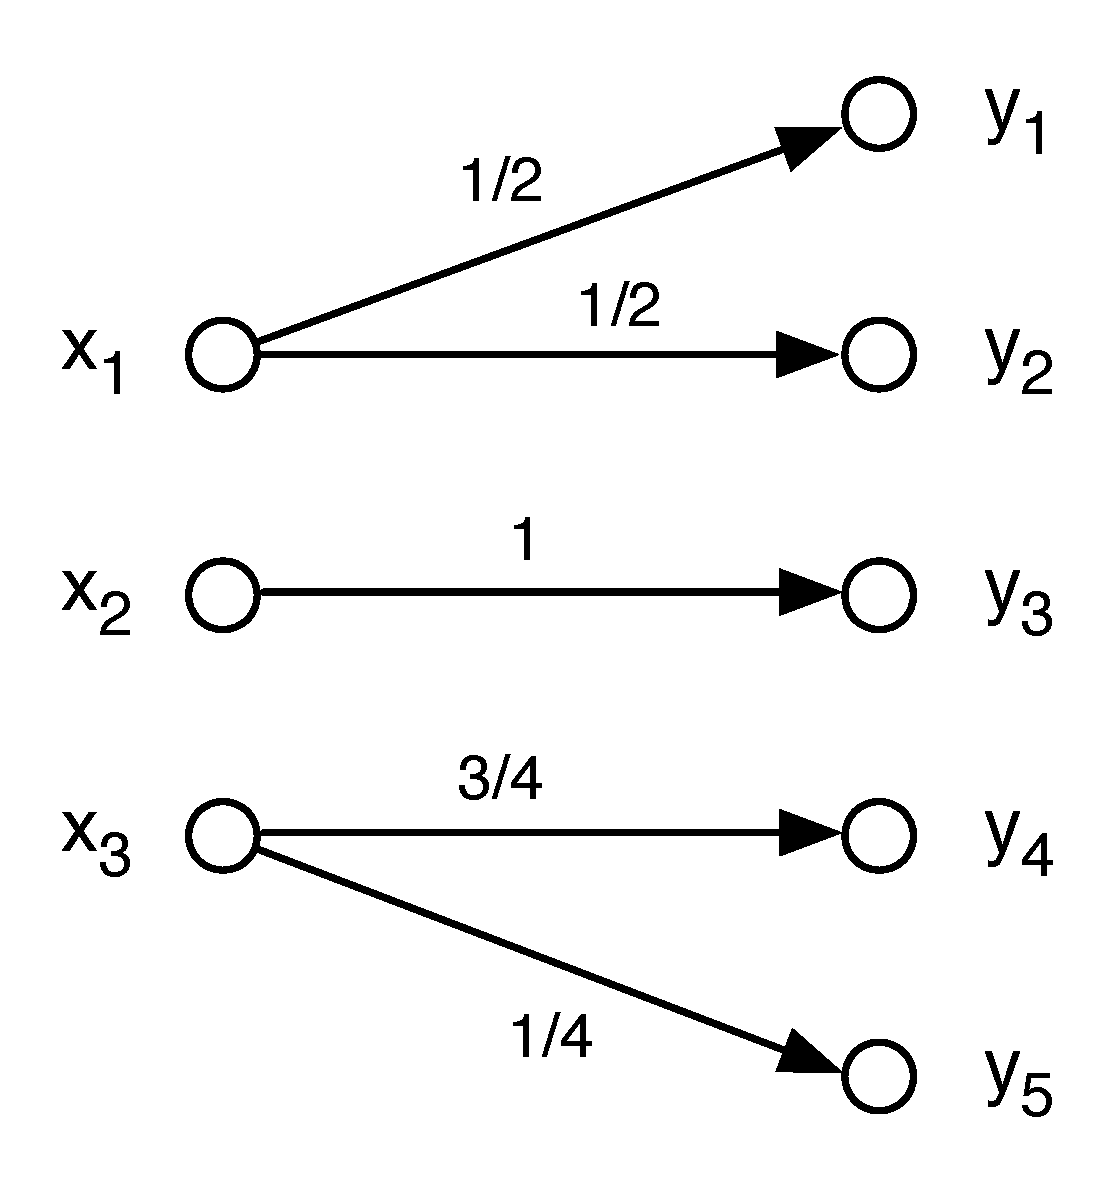
\includegraphics[width=0.4\textwidth]{img/noiseless1.pdf}}        
  \hspace{1cm}
  \subfloat[Matrice di canale]{\label{fig:noiseless2}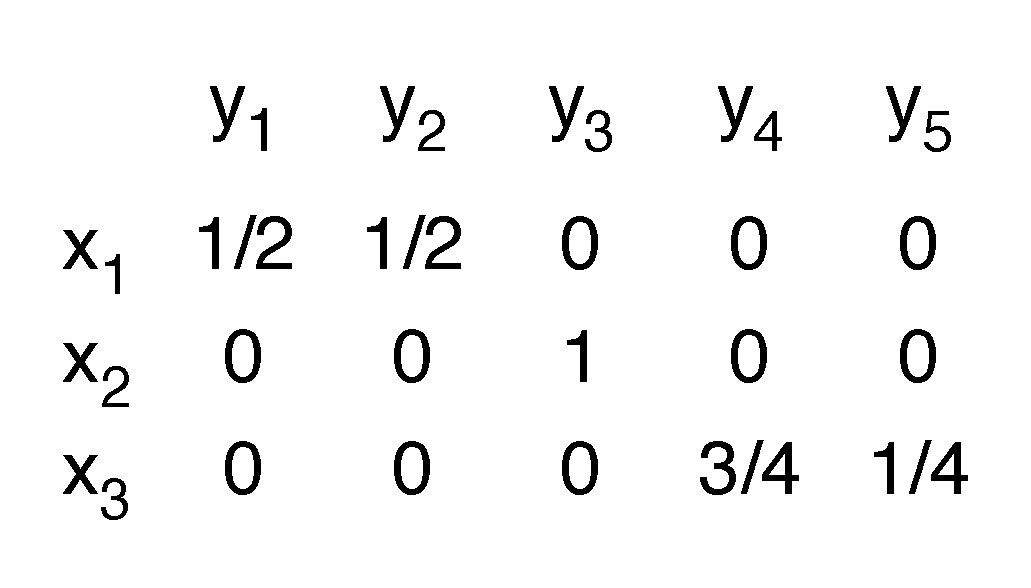
\includegraphics[width=0.4\textwidth]{img/noiseless2.pdf}}
  \caption{Esempio di canale noiseless}
  \label{fig:noiseless}
\end{figure}

\begin{lemma}
 Se $\mathcal{C}$ è noiseless, allora $H(X/Y)=0$
 \begin{proof}
 Supponiamo per comodità
 che $\forall y \in Y p(y)>0$. Se così non fosse, sarebbe sufficiente rimuovere il simbolo (non c'è quindi perdita di generalità).
 Dalla definizione di entropia condizionata:
 \[
  H(X/Y)=\sum_{y \in Y} p(y)H(X/Y=y)
 \]
 Poiché abbiamo supposto $p(y)>0$, bisogna dimostrare che:
 \[
  \forall y \in Y \ : \ H(X/Y=y)=\sum_{x \in X}p(x/y) log( p(x/y)) =0
 \]
 Chiaramente l'uguaglianza vale se: 
 \[
  \forall x \in X, \forall y \in Y \ : \ p(x/y)=0 \lor p(x/y)=1
 \]
 In maniera intuitiva però ciò è vero, è sufficiente infatti osservare il grafo di canale. Preso un certo y, esiste un unico 
 arco che lo connette ad un certo x (il caso con probabilità 1), mentre nessun arco che lo connette ad altri x (i casi con 
 probabilità 0).
 In maniera più formale, chiamiamo $x(y)$ l'unico $x$ per cui $p(y/x)>0$ (ne esiste uno solo per la def. di canale noiseless).
 Ora:
 \[
  p(x/y)=\frac{p(y/x)p(x)}{p(y)}=\frac{p(y/x)p(x)}{ \displaystyle\sum_{z \in X} p(y/z)p(z)}=
  \frac{p(y/x)p(x)}{ p(y/x(y))p(x(y))}
 \]
 A questo punto se x=x(y) si ottiene:
 \[
  p(x(y)/y)=\frac{p(y/x(y))p(x(y))}{ p(y/x(y))p(x(y))}=1
 \]
 Mentre se $x\neq x(y)$:
 \[
  p(x/y)=\frac{0 p(x)}{ p(y/x(y))p(x(y))}=0
 \]
 \end{proof}
\end{lemma}

\noindent
Calcoliamo ora la capacità per un canale noiseless.

\begin{lemma}
Se \mathcal{C} è noiseless, allora $C=log|X|$
\begin{proof}
 \[
  C=\max_{p(x)} I(X;Y)=\max_{p(x)} H(X)-H(X/Y)
 \]
 Ora per il lemma precedente H(X/Y) è 0, da cui:
 \[
  C=\max_{p(x)} H(X)-H(X/Y)=\max_{p(x)} H(X)
 \]
 Ma il massimo della funzione entropia è il logaritmo del numero di valori, che 
 si ha nel caso di distribuzione uniforme (proposizione \ref{propen}), quindi:
 \[
  C=\max_{p(x)} H(X)=log|X|
 \]
\end{proof}
\end{lemma}

\subsection{Canale deterministico}

\medskip

\begin{definizione}
 Un canale si dice deterministico (molti a uno) se:
\[
 \forall x \in X \exists ! \ y \in Y \ : \ p(y/x) > 0
\]
Ovvero se:
\[
 \forall x \in X \exists ! \ y \in Y \ : \ p(y/x)=1
\]
\end{definizione}

In questo caso la situazione è quindi opposta a prima. E' il mittente che sa sempre che simbolo viene ricevuto, mentre 
il destinatario non sa cosa è stato inviato.
In figura \ref{fig:deterministico} è riportato un esempio di canale deterministico.

\begin{figure}[htbp]
  \centering
  \subfloat[Grafo di canale]{\label{fig:determ1}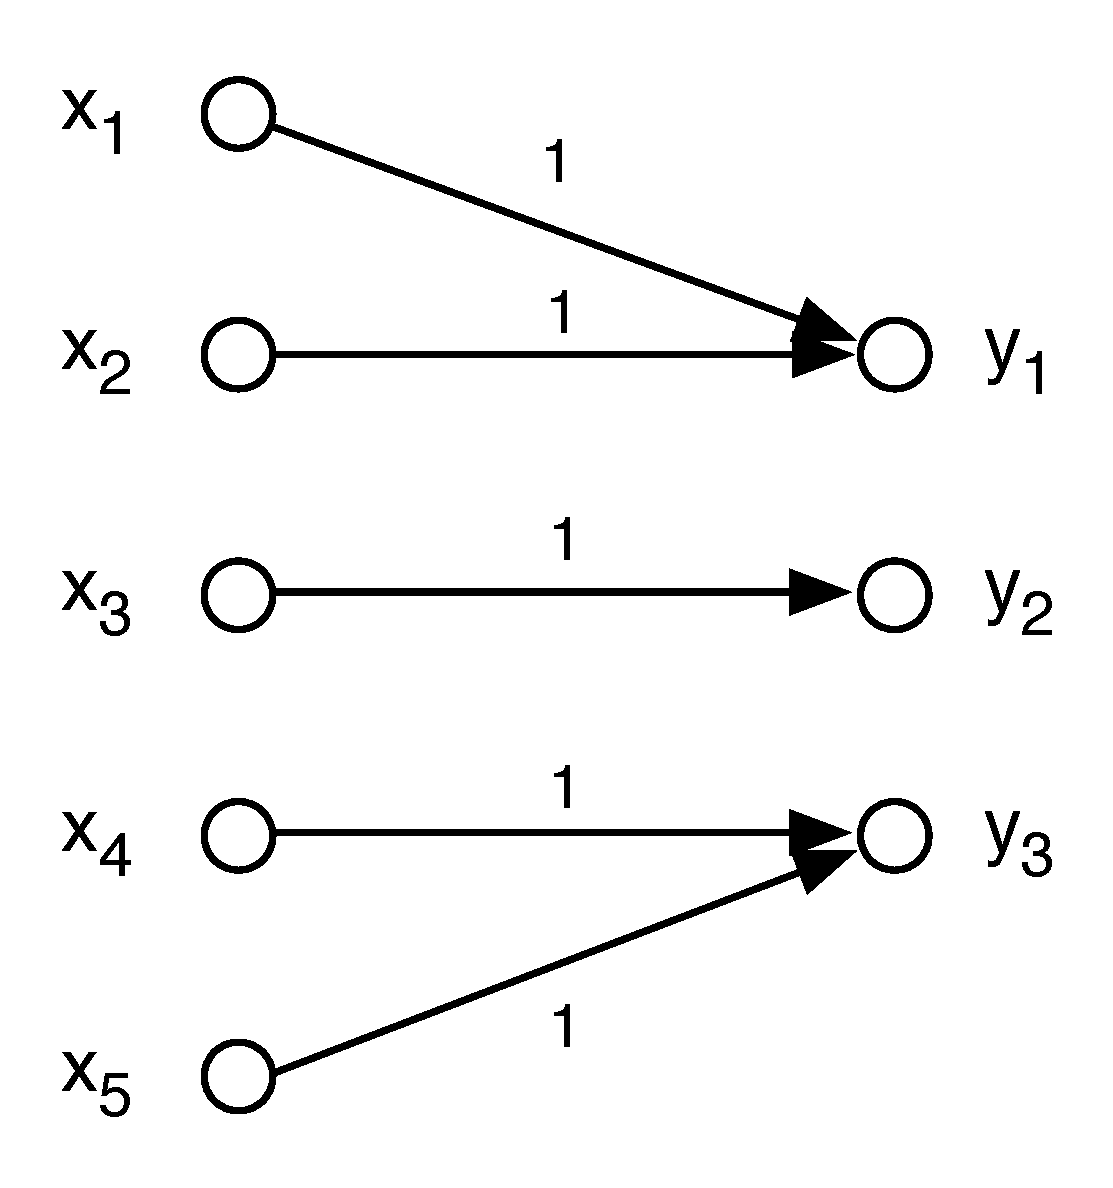
\includegraphics[width=0.4\textwidth]{img/determ1.pdf}}        
  \hspace{1cm}
  \subfloat[Matrice di canale]{\label{fig:determ2}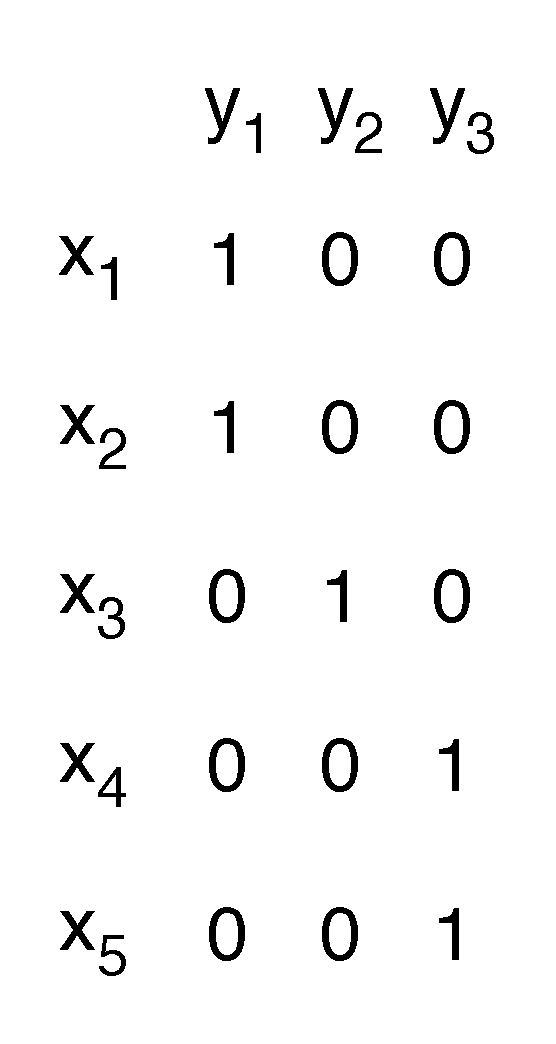
\includegraphics[width=0.25\textwidth]{img/determ2.pdf}}
  \caption{Esempio di canale deterministico}
  \label{fig:deterministico}
\end{figure}

\begin{lemma}
 Se \mathcal{C} è deterministico, allora $H(Y/X)=0$
 \begin{proof}
  \[
   H(Y/X)=\sum_{x \in X} p(x)H(Y/X=x)
  \]
  Ma $\forall x \in X$, H(Y/X=x)=0. Infatti:
  \[
   H(Y/X=x)=\sum_{y \in Y}p(y/x) log(p(y/x))
  \]
  E per la definizione di canale deterministico $p(y/x)=0 \lor p(y/x)=1$
 \end{proof}
\end{lemma}

Calcoliamo ora la capacità per un canale deterministico.

\begin{lemma}
Se \mathcal{C} è deterministico, allora $C=log|Y|$
\begin{proof}
 \[
  C=\max_{p(x)} I(X;Y)=\max_{p(x)} H(Y)-H(Y/X)
 \]
 Ora per il lemma precedente H(Y/X) è 0, da cui:
 \[
  C=\max_{p(x)} H(X)-H(X/Y)=\max_{p(x)} H(Y)
 \]
 Analogamente al canale noiseless, si ha il massimo che è pari al logaritmo, con distribuzione uniforme:
 \[
  C=\max_{p(x)} H(Y)=log|Y|
 \]
 Tuttavia questa volta la distribuzione uniforme deve essere p(y)!
 L'ultima considerazione è dunque valida se esiste una distribuzione p(x), tale che p(y) sia uniforme.
 Poniamo:
 \[
  X(y)=\{x \in X \ / \ p(y/x)=1 \}
 \]
 Allora la distribuzione p(x) che rende uniforme p(y) è:
 \[
  p(x)=\frac{1}{|Y| \ |X(y)|}
 \]
 Ciò è vero in quanto:
 \[\begin{split}
  p(y)&=\sum_{x \in X}p(x)p(y/x) \\
      &=\sum_{x \in X(y)}p(x) \\
      &=\sum_{x \in X(y)}\frac{1}{|Y| \ |X(y)|} \\
      &=\frac{1}{|Y|} \frac{|X(y)|}{|X(y)|} \\
      &=\frac{1}{|Y|}
   \end{split}
 \]

\end{proof}
\end{lemma}


\subsection{Canale completamente deterministico}

\medskip

\begin{definizione}
 Un canale si dice completamente deterministico (uno a uno) se è noiseless e deterministico.
\end{definizione}

In questo caso quindi sia il mittente che il destinatario sanno cosa è stato ricevuto/inviato.
In figura \ref{fig:cdeterministico} è riportato un esempio di canale completamente deterministico.

\begin{figure}[htbp]
  \centering
  \subfloat[Grafo di canale]{\label{fig:cdeterm1}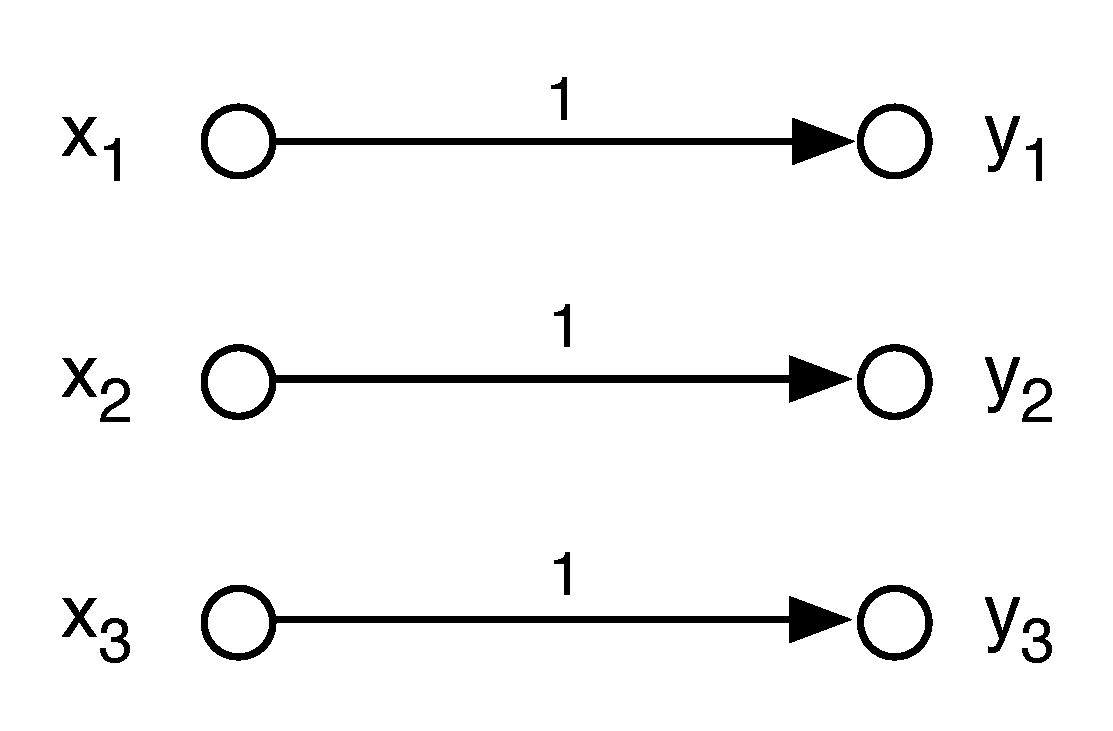
\includegraphics[width=0.4\textwidth]{img/cdeterm1.pdf}}        
  \hspace{1cm}
  \subfloat[Matrice di canale]{\label{fig:cdeterm2}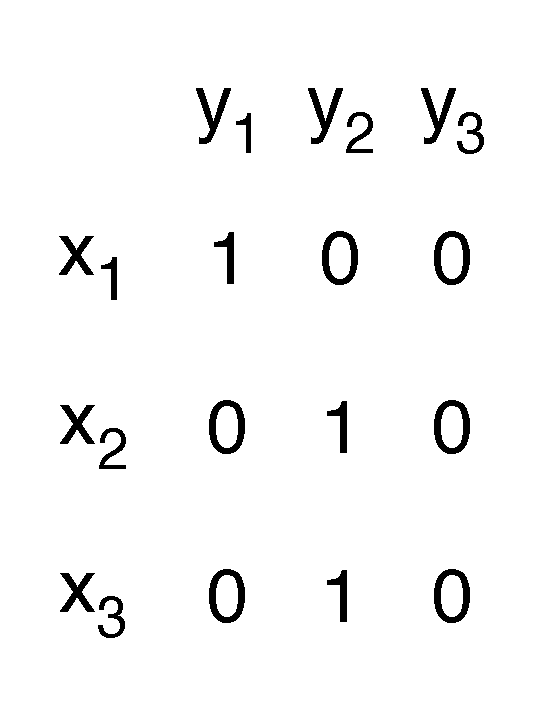
\includegraphics[width=0.25\textwidth]{img/cdeterm2.pdf}}
  \caption{Esempio di canale completamente deterministico}
  \label{fig:cdeterministico}
\end{figure}

\begin{lemma}
 Se \mathcal{C} è completamente completamente deterministico, allora:
 \begin{itemize}
  \item $H(Y/X)=H(X/Y)=0$
  \item $I(X;Y)=H(X)=H(Y)$
 \end{itemize}
 \begin{proof}
  Il primo punto segue direttamente dai lemmi per il canale noiseless e deterministico.
  Il secondo punto è la solita proprietà dell'informazione mutua:
  \[\begin{split}
   I(X;Y)&=H(X)-H(X/Y)=H(X) \\
   I(X;Y)&=H(Y)-H(Y/X)=H(Y)
   \end{split}
  \]

 \end{proof}
\end{lemma}

\noindent
Per quanto riguarda infine la capacità di canale:

\begin{lemma}
Se \mathcal{C} è completamente deterministico, allora $C=log|X|=log|Y|$
\begin{proof}
Segue direttamente dai lemmi per il canale noiseless e deterministico.
\end{proof}
\end{lemma}



\subsection{Canale inutile}

\medskip

\begin{definizione}
 Un canale si dice inutile (molti a molti) se:
 \[
  \forall y \in Y \ \exists C(y) \in R \ : \ \forall x \in X p(y/x)=C(y)
 \]
 Dove C(y) è una costante che dipende da y.
\end{definizione}

In questo caso quindi le colonne della matrice di canale sono costanti, quindi le righe sono tutte identiche fra loro.
In figura \ref{fig:inutile} è riportato un esempio di canale inutile. Osservando il grafo di canale (o la matrice) è facile capire
come mai il canale è detto ``inutile''. Infatti il mittente ed il destinatario non potranno derivare alcuna informazione dalla 
comunicazione...che è stata appunto inutile.

\begin{figure}[htbp]
  \centering
  \subfloat[Grafo di canale]{\label{fig:inutile1}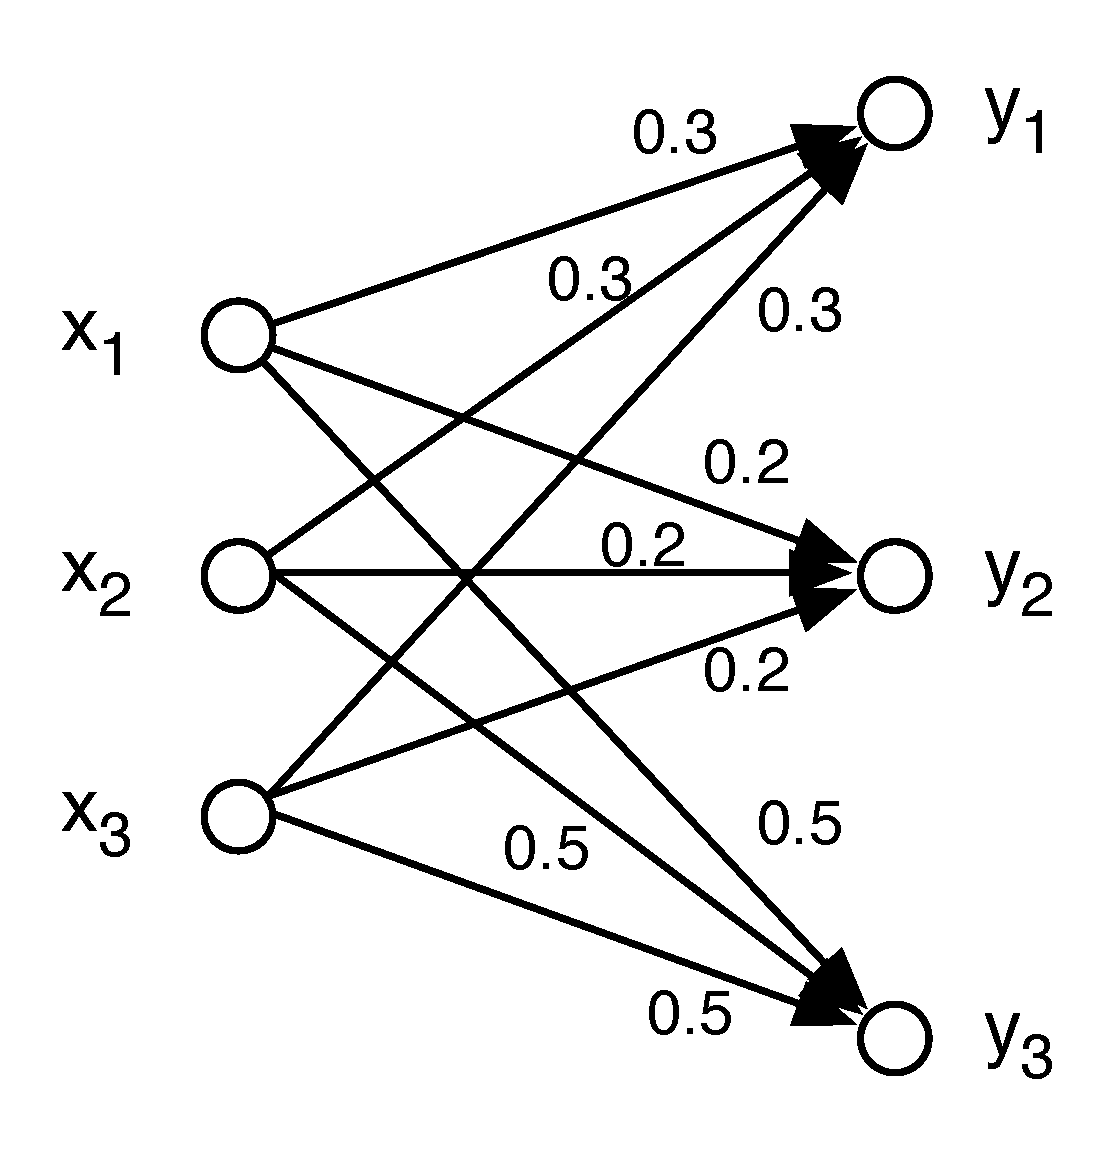
\includegraphics[width=0.5\textwidth]{img/inutile1.pdf}}        
  \hspace{1cm}
  \subfloat[Matrice di canale]{\label{fig:inutile2}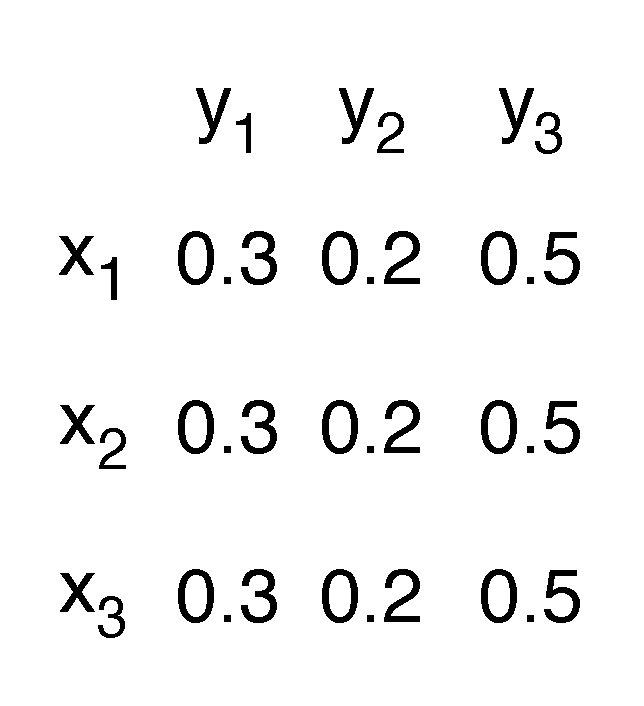
\includegraphics[width=0.25\textwidth]{img/inutile2.pdf}}
  \caption{Esempio di canale inutile}
  \label{fig:inutile}
\end{figure}

\begin{lemma}
 Se \mathcal{C} è inutile, allora:
\[
  I(X;Y)=0
\]
 \begin{proof}
\[\begin{split}
 p(x,y)&=p(x)p(y/x) \\
       &=p(x)p(y/x)\sum_{x \in X}p(x) 
       =p(x)C(y)\sum_{x \in X}p(x) \\
       &=p(x) \sum_{x \in X}p(x)C(y)
       =p(x) \sum_{x \in X}p(x)p(y/x)\\
       &=p(x) p(y) \\
  \end{split}
\]
Quindi $p(x,y)=p(x)p(y)$, il che implica che X e Y sono indipendenti.
Ma se X e Y sono indipendenti, per l'osservazione \ref{mutuaindip} si ha I(X;Y)=0
 \end{proof}
\end{lemma}

\noindent
Per quanto riguarda infine la capacità di canale:

\begin{lemma}
Se \mathcal{C} è inutile, allora $C=0$
\begin{proof}
Segue direttamente dal lemma precedente.
\end{proof}
\end{lemma}

\subsection{Canale simmetrico}

\medskip

\begin{definizione}
 Un canale si dice simmetrico se:
 \begin{enumerate}
  \item Le righe nella sua matrice di canale sono uguali a meno di una permutazione
  \item Le colonne nella sua matrice di canale sono uguali a meno di una permutazione
 \end{enumerate}
\end{definizione}


\begin{table}[htbp]
  \begin{center}
   \begin{tabular}{c c c c}
	& $y_1$ & $y_2$ & $y_3$ \\
	$x_1$ & 0.3 & 0.2 & 0.5 \\ 
	$x_2$ & 0.5 & 0.3 & 0.2  \\ 
	$x_3$ & 0.2 & 0.5 & 0.3  \\ 
    \end{tabular}
  \caption{Esempio di canale simmetrico (Matrice di canale).}
  \label{tab:tsim}
  \end{center}
\end{table}

\begin{lemma}
 Se \mathcal{C} è un canale simmetrico, c una riga ed r una colonna della sua matrice di canale, allora:
 \begin{enumerate}
  \item $H(Y/X)=H(r)$
  \item $H(X/Y)=H(c)$
 \end{enumerate}
 \begin{proof}
  \mbox{}

  \noindent
  Per quanto riguarda il primo punto:
  \[
   H(Y/X)=\sum_{x \in X}p(x)H(Y/X=x)
  \]
  Ma le righe sono tutte uguali a meno di una permutazione, quindi H(Y/X=x) è costante, da cui:
  \[
   H(Y/X)=H(r)\sum_{x \in X}p(x)=H(r)
  \]
  Il secondo punto è del tutto analogo, visto che anche le colonne sono uguali a meno di una permutazione.
 \end{proof}

\end{lemma}

\noindent
Un esempio di canale simmetrico è riportato in tabella \ref{tab:tsim}.
La capacità di un canale simmetrico è fornita dal seguente teorema

\begin{teorema}
 Se \mathcal{C} è un canale simmetrico ed r una riga della matrice di canale di \mathcal{C}, allora:
 \[
  C=log|Y| - H(r)
 \]
 \begin{proof}
\[
  C=\max_{p(x)} I(X;Y)=\max_{p(x)} H(Y)-H(Y/X)
\]
 Ora per il lemma precedente:
 \[
  \max_{p(x)} H(Y)-H(Y/X)=\max_{p(x)} H(Y)-H(r)
 \]
 H(r) non dipende da p(x), quindi basta massimizzare H(Y) che come già visto ha massimo in $log|Y|$. Quindi:
 \[
  C=\max_{p(x)} H(Y)-H(r)=log |Y| - H(r)
 \]
 Il risultato si ottiene, come già visto per il canale deterministico, quando p(y) ha distribuzione uniforme.
 Tuttavia in questo caso anche p(x) deve essere uniforme. Infatti:
 \[
  p(x)=\frac{1}{|X|} \Rightarrow p(y)=\frac{1}{|Y|}
 \]
 Ciò si ricava facilmente da:
 \[
  p(y)=\sum_{x \in X} p(x)p(y/x)=\frac{1}{|X|} \sum_{x \in X}p(y/x)
 \]
 Ma la somma degli elementi di ogni colonna è costante, quindi:
 \[
  \frac{1}{|X|} \sum_{x \in X}p(y/x)=\frac{1}{|X|} const=\frac{1}{|Y|}
 \]
 \end{proof}

\end{teorema}

\subsection{Canale debolmente simmetrico}

\medskip

\begin{definizione}
 Un canale si dice debolmente simmetrico se:
 \begin{enumerate}
  \item Le righe nella sua matrice di canale sono uguali a meno di una permutazione
  \item La somma degli elementi di ciascuna colonna nella sua matrice di canale è costante
 \end{enumerate}
\end{definizione}

\begin{table}[htbp]
  \begin{center}
   \begin{tabular}{c c c c}
	  & $y_1$ & $y_2$ & $y_3$ \\
	$x_1$ & 1/3 & 1/6 & 1/2 \\ 
	$x_2$ & 1/3 & 1/2 & 1/6  \\ 
    \end{tabular}
  \end{center}
  \label{tdsim}
  \caption{Esempio di canale debolmente simmetrico (Matrice di canale).}
\end{table}

\noindent
Un esempio di canale debolmente simmetrico è riportato in tabella \ref{tdsim}.
La capacità di canale è uguale a quella dei canali simmetrici, come descritto dal seguente teorema.

\begin{teorema}
 Se \mathcal{C} è un canale debolmente simmetrico ed r una riga della matrice di canale di \mathcal{C}, allora:
 \[
  C=log|Y| - H(r)
 \]
 Il risultato si ottiene quando p(x) è uniforme.
\begin{proof}
 E' esattamente identica a quella del canale simmetrico.
\end{proof}

\end{teorema}

\subsection{Binary Symmetric Channel}

Il Binary Symmetric Channel (BSC) è un particolare canale simmetrico composto da due simboli in ingresso e da due simboli in uscita (ne avevamo già visto un esempio in introduzione, figura \ref{fig:bsc}).

\begin{figure}[htbp]
  \centering
  \subfloat[Grafo di canale]{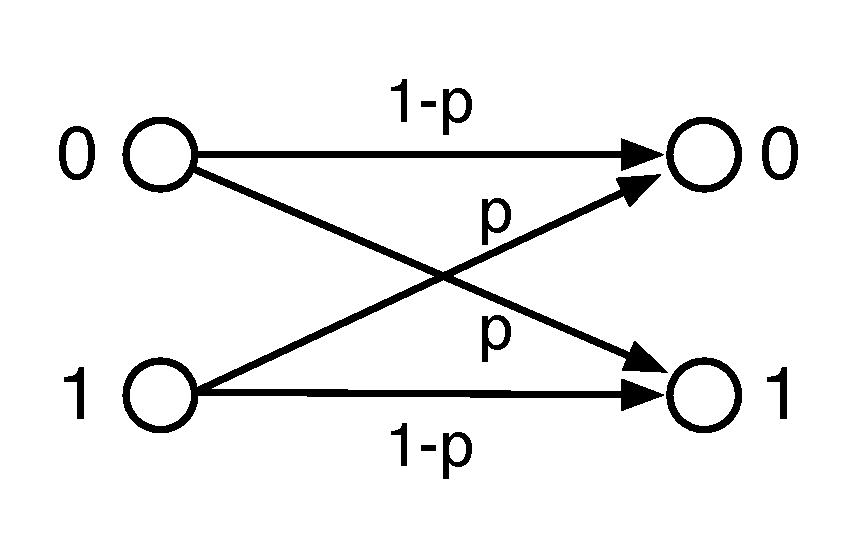
\includegraphics[width=0.4\textwidth]{img/bsc1.pdf}}        
  \hspace{1cm}
  \subfloat[Matrice di canale]{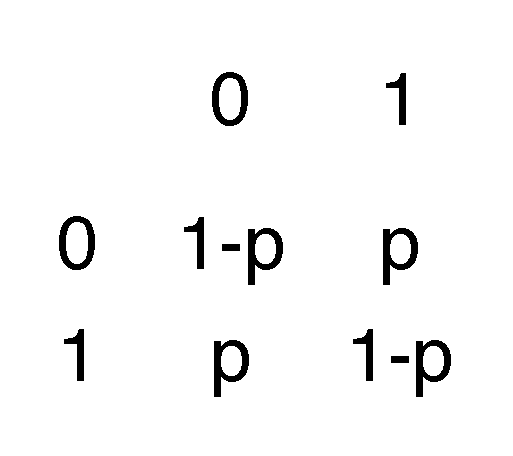
\includegraphics[width=0.25\textwidth]{img/bsc2.pdf}}
  \caption{BSC}
  \label{fig:bsc2}
\end{figure}

Il canale è rappresentato in figura \ref{fig:bsc2}. Con p abbiamo quindi indicato la probabilità che ci sia un errore di trasmissione.
Siamo ora interessati a calcolare la capacità di questo canale.
Innanzitutto indichiamo con $\Pi$ la probabilità che la sorgente emetta il simbolo 0, ovvero:
\[
 \Pi=P\{X=0\}
\]
Calcoliamo ora l'informazione mutua:
\[
 I(X;Y)=H(Y)-H(Y/X)
\]
Calcoliamo il primo termine. In questo caso la variabile Y ha due simboli, quindi l'entropia 
sarebbe formata da due elementi (Y=0 e Y=1), tuttavia ne indichiamo solo uno (Y=1). L'altro infatti si può ricavare 
al solito come differenza, tenendo conto che la somma è 1. 
\[
 H(Y)=H(\Pi p + (1-\Pi)(1-p))
\]
Per il secondo termine:
\[\begin{split}
 H(Y/X)&=\Pi H(Y/X=0) + (1-\Pi) H(Y/X=1) \\
       &=\Pi H(p) + (1-\Pi) H(p) \\
       &=H(p)
  \end{split}
\]
A questo punto la capacità di canale è:
\[
 C=\max_{p(x)} I(X;Y)=\max_{0 \le \Pi \le 1} I(X;Y)=\max_{0 \le \Pi \le 1} [ H(\Pi p + (1-\Pi)(1-p)) - H(p) ]
\]
Dobbiamo ora trovare il valore di $\Pi$ che massimizza l'informazione mutua, ovvero:
\[
 arg \max_{0 \le \Pi \le 1} [ H(\Pi p + (1-\Pi)(1-p)) - H(p) ]
\]
Ma H(p) non dipende da $\Pi$, quindi basta risolvere:
\[
 arg \max_{0 \le \Pi \le 1} [ H(\Pi p + (1-\Pi)(1-p))]
\]
Ma sappiamo che l'entropia raggiunge il massimo quando le componenti sono equiprobabili.
In questo caso abbiamo due componenti, quindi deve essere:
\[\begin{split}
 &\Pi p + (1-\Pi)(1-p)=\frac{1}{2} \\
 \Rightarrow &\Pi p + 1-p + -\Pi +\Pi p=\frac{1}{2} \\ 
 \Rightarrow &\Pi(2p-1) + 1-p =\frac{1}{2} \\ 
 \Rightarrow &\Pi(2p-1) =\frac{1}{2}-1+p \\ 
 \Rightarrow &\Pi(2p-1) =-\frac{1}{2}+p \\
 \Rightarrow &\Pi=\frac{-\frac{1}{2}+p}{2p-1} \\  
 \Rightarrow &\Pi=\frac{p-\frac{1}{2}}{2(p-\frac{1}{2})} \\
 \Rightarrow &\Pi=\frac{1}{2} \\
  \end{split}
\]

\noindent
Dunque si ha il massimo quando $\Pi=1/2$, ovveroquando la sorgente emette in maniera equiprobabile 0 o 1.
Infine, poiche $H(1/2,1/2)=1$, la capacità di canale di un BSC è:

\[
 C=1-H(p)
\]

In figura \ref{fig:cbsc} è rappresentata la capacità del canale, al variare di p.
Come si nota quando p=0 (o p=1) la capacità è massima, infatti sul canale circola un grande contenuto informativo, non c'è infatti 
alcuna incertezza. Viceversa quando p=1/2 sul canale non viaggia alcuna informazione. Il destinatario infatti alla ricezione di un simbolo non è in grado di inferire nulla (in questo caso si ha un canale inutile).

\begin{figure}[htbp]
\begin{center}
	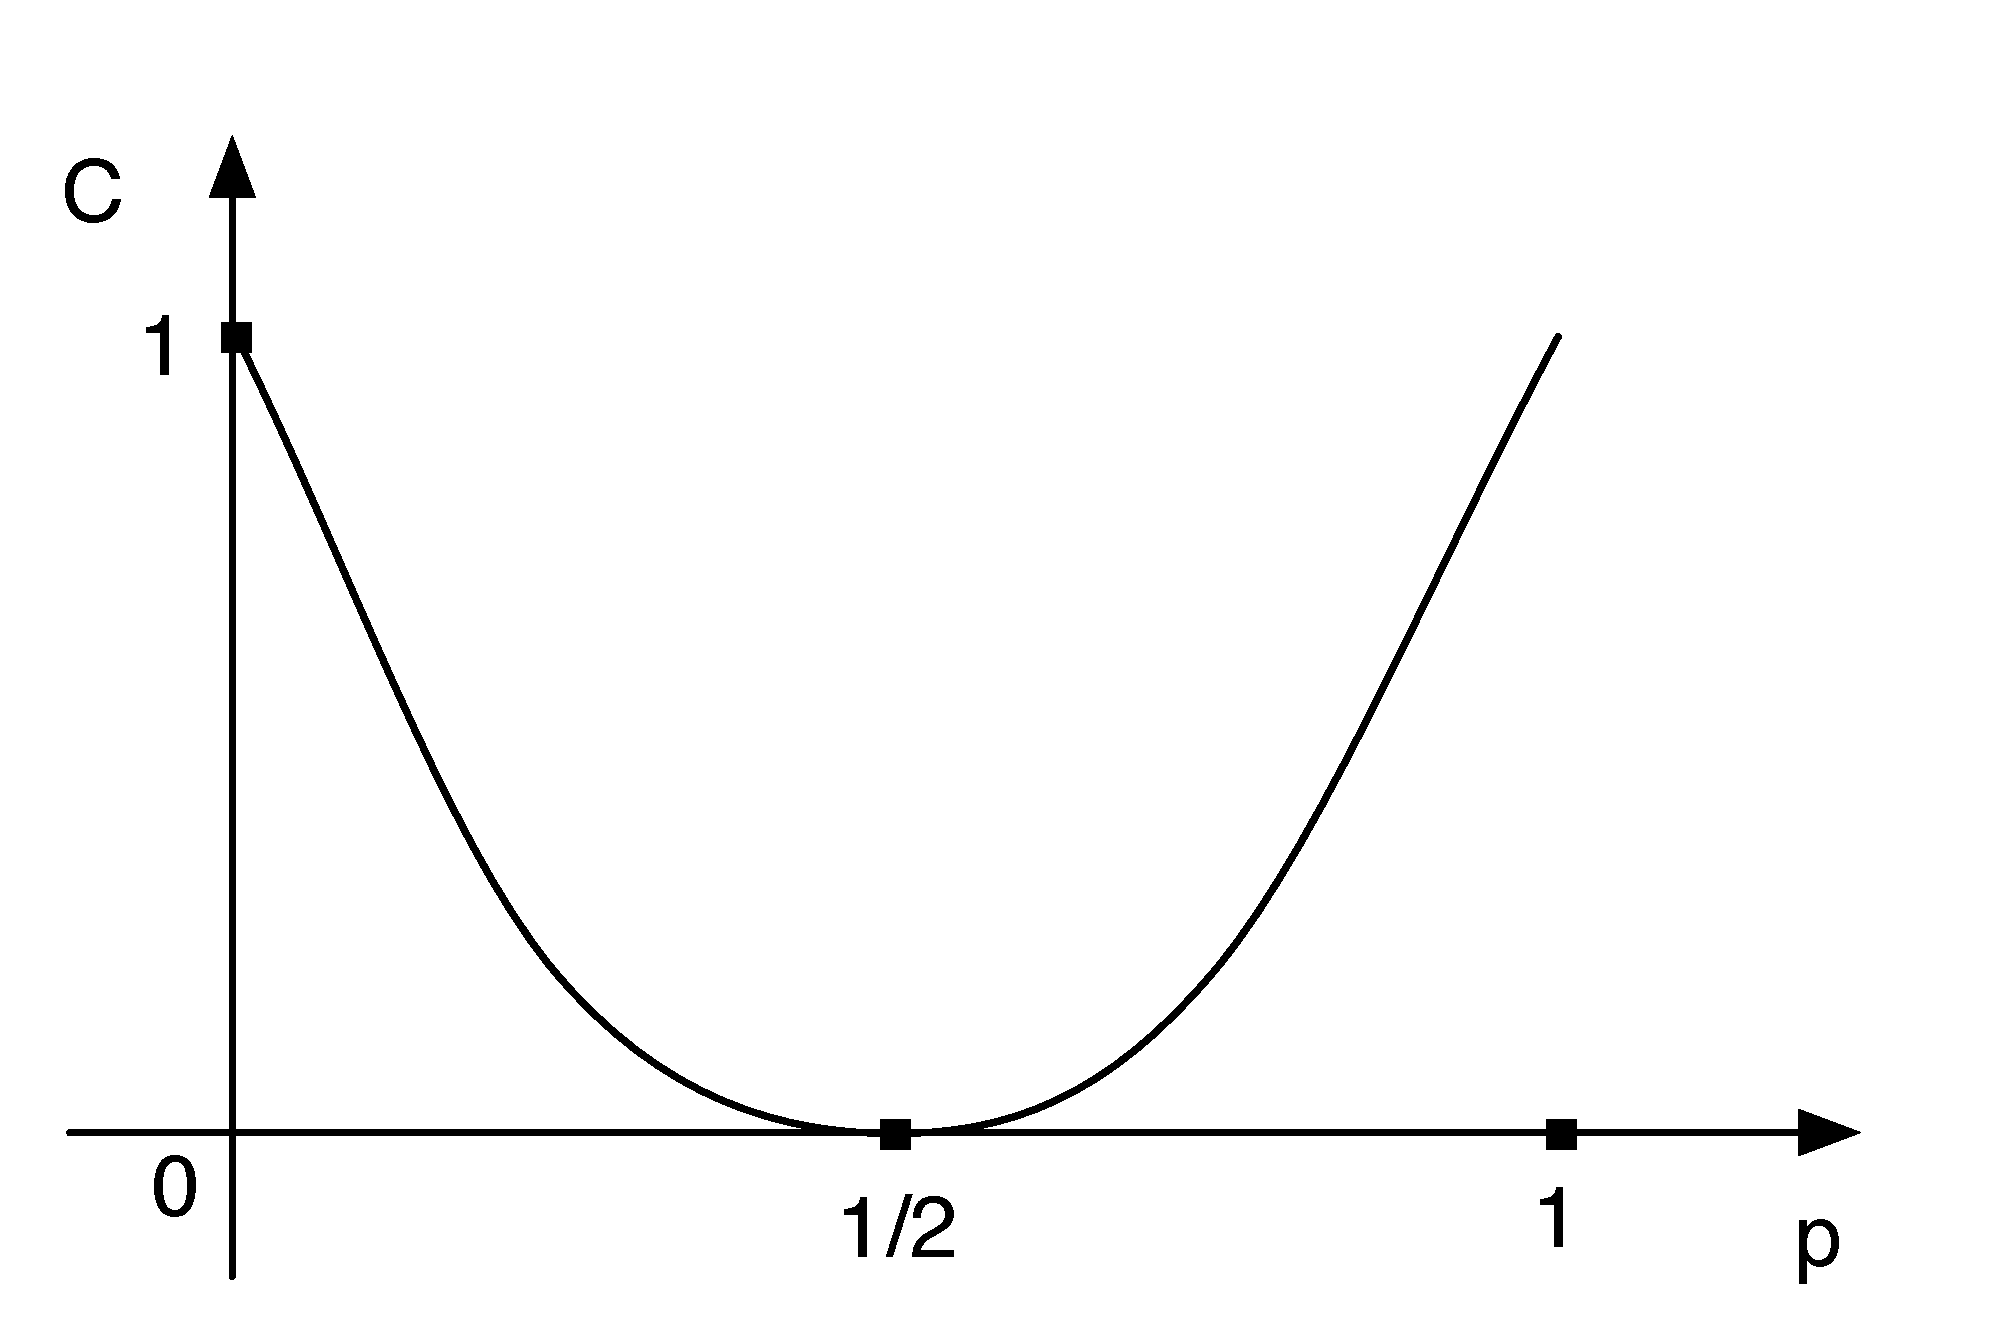
\includegraphics[width=0.6\textwidth]{img/cbsc.pdf}
\caption{Capacità di canale di un BSC al variare di p}
\label{fig:cbsc}
\end{center}
\end{figure}

\newpage

\subsection{Binary Erasure Channel}
Nel Binary Erasure Channel (BEC), il mittente può inviare due diversi simboli al destinatario. Un simbolo può essere ricevuto 
correttamente oppure ``perso'' (in questo caso il destinatario riceve uno speciale simbolo $\sharp$). Il canale ha dunque 2 ingressi, 3 uscite 
ed un parametro p che indica la probabilità di ``perdere'' il simbolo. Il canale è rappresentato in figura \ref{fig:bec}.

\begin{figure}[htbp]
  \centering
  \subfloat[Grafo di canale]{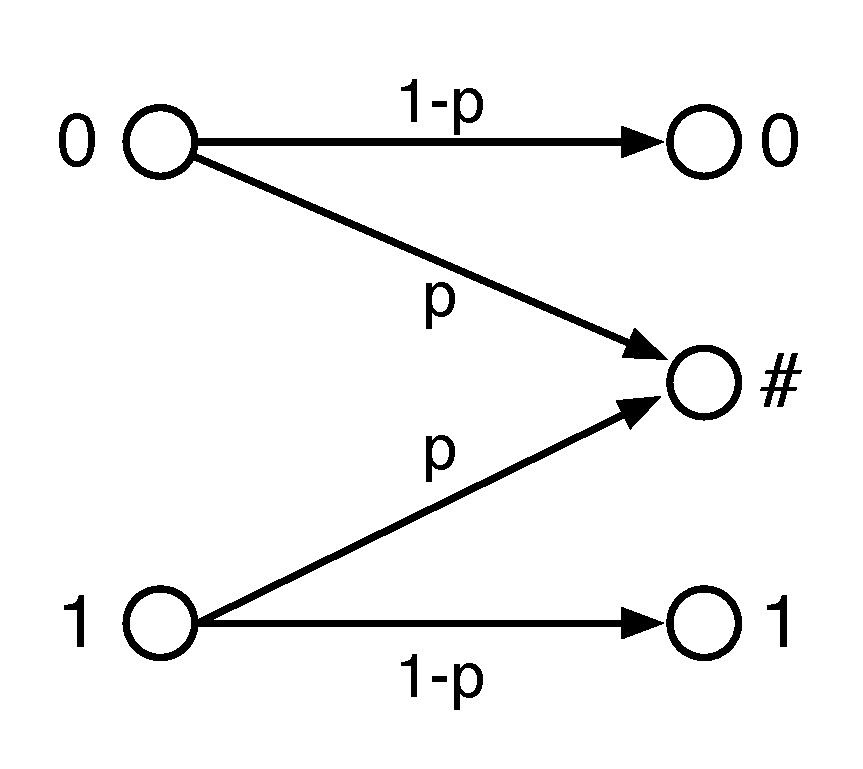
\includegraphics[width=0.35\textwidth]{img/bec1.pdf}}        
  \hspace{1cm}
  \subfloat[Matrice di canale]{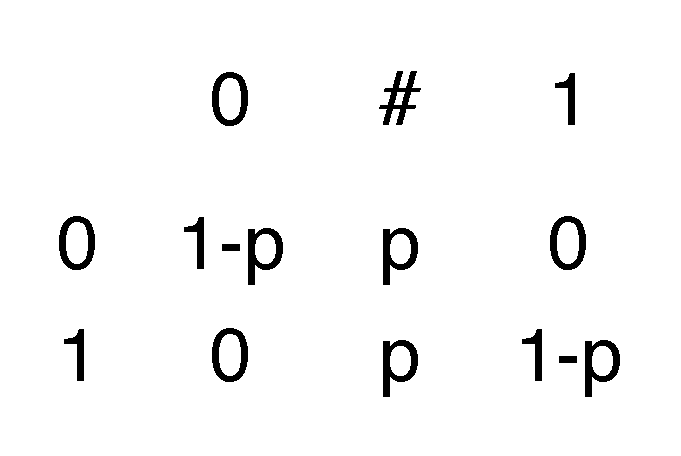
\includegraphics[width=0.26\textwidth]{img/bec2.pdf}}
  \caption{BEC}
  \label{fig:bec}
\end{figure}

\noindent
Procediamo al calcolo della capacità di canale. Come per il BSC poniamo:
\[
 \Pi=P\{X=0\}
\]
Ora per calcolare l'informazione mutua ricaviamo:
\[
 H(Y)=H(Y=0,Y=1,Y=\sharp)=H(\Pi (1-p), (1-\Pi) (1-p), p)
\]
E:
\[\begin{split}
 H(Y/X)&=\Pi H(Y/X=0) + (1-\Pi) H(Y/X=1) \\
       &=\Pi H(1-p,p,0) + (1-\Pi) H(0,p,1-p) \\
       &=\Pi H(p) + (1-\Pi) H(p) \\
       &=H(p)
  \end{split}
\]
Quindi:
\[
 I(X;Y)=H(Y)-H(Y/X)=H(\Pi (1-p), (1-\Pi) (1-p), p) - H(p)
\]
La capacità di canale è dunque:
\[
 C=\max_{0 \le \Pi \le 1} H(\Pi (1-p), (1-\Pi) (1-p), p) - H(p)
\]
In maniera analoga al BSC, H(p) non dipende da $\Pi$, quindi per massimizzare 
l'informazione mutua bisogna massimizzare la prima entropia.
Ma sappiamo che la funzione entropia è continua e concava (oss. \ref{entrconcava}).
Quindi esiste un solo massimo, quando la derivata è 0. Calcoliamo allora la derivata
(poniamo per brevità q=1-p):

\[\begin{split}
 &\frac{d}{d \Pi}  H(\Pi (1-p), (1-\Pi) (1-p), p) \\
 =&\frac{d}{d \Pi} H(\Pi q, (1-\Pi) q, p) \\
 =&\frac{d}{d \Pi} - [ \ \Pi q log(\Pi q) + (1-\Pi) q log((1-\Pi)q) + plog(p) \ ] \\
 =&-[\Pi q \frac{1}{\Pi q} q + q log(\Pi q) + (1-\Pi)q \frac{1}{(1-\Pi)q} (-q) + -qlog((1-\Pi)q) ] \\
 =&-[q + q log(\Pi q) -q -qlog((1-\Pi)q) ] \\
 =&-q[log(\Pi q) -log((1-\Pi)q) ] \\
 =&-qlog \frac{\Pi q}{(1-\Pi)q}=-qlog \frac{\Pi}{1-\Pi}
  \end{split}
\]
Ora eguagliamo la derivata a 0 e ricaviamo $\Pi$:
\[\begin{split}
 &-qlog \frac{\Pi}{1-\Pi}=0 \\
 \Rightarrow &\frac{\Pi}{1-\Pi}=1 \\
 \Rightarrow &\Pi=1-\Pi \\
\Rightarrow &\Pi=\frac{1}{2}
  \end{split}
\]
Quindi si ha il massimo quando $\Pi=\frac{1}{2}$.
La capacità di canale è dunque (si ponga sempre attenzione al fatto che come al solito H(p)=H(p,1-p) ):
\[\begin{split}
C=&H(\frac{1}{2} q, \frac{1}{2} q, p) - H(p) \\
=& -\frac{q}{2} log\frac{q}{2} - \frac{q}{2} log\frac{q}{2}  - plog(p) +p log(p) +q log(q)\\
=&-qlog\frac{q}{2}+q log(q)  \\
=&qlog(2) -qlog(q) +q log(q)\\
=&qlog(2) \\
=&q=1-p
\end{split}
\]

\subsection{Canale Z}
Il canale Z è composto da 2 simboli. Un simbolo arriva con certezza in maniera corretta al destinatario, mentre l'altro può essere 
tramutato nel primo con probabilità (quindi di errore) p. Il canale è rappresentato in figura \ref{fig:z}.

\begin{figure}[htbp]
  \centering
  \subfloat[Grafo di canale]{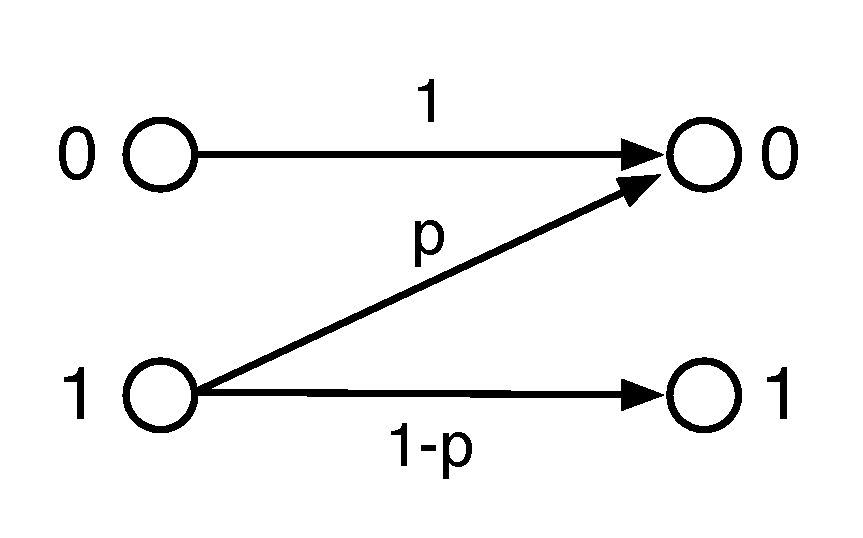
\includegraphics[width=0.35\textwidth]{img/z1.pdf}}        
  \hspace{1cm}
  \subfloat[Matrice di canale]{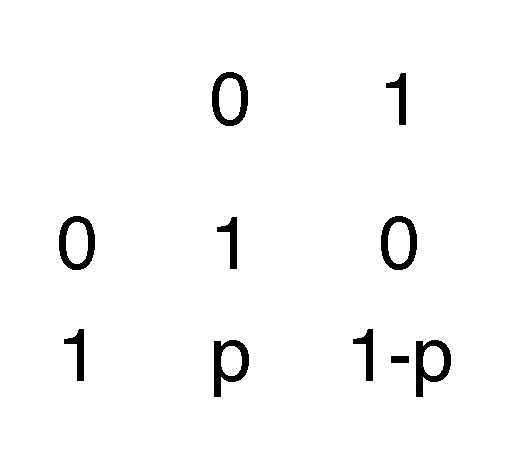
\includegraphics[width=0.26\textwidth]{img/z2.pdf}}
  \caption{Canale Z}
  \label{fig:z}
\end{figure}

\noindent
Calcoliamo ora la capacità del canale Z.
Poniamo (diversamente da prima!):
\[
 \Pi=P\{X=1\}
\]
Ora per calcolare l'informazione mutua ricaviamo:
\[\begin{split}
 H(Y)=&H(1-\Pi+\Pi p,\Pi (1-p)) \\
     =&H(1-\Pi(1-p),\Pi(1-p)) \\
     =&H(\Pi(1-p))
  \end{split}
\]
E:
\[\begin{split}
 H(Y/X)=&\Pi H(Y/X=1)+(1-\Pi)H(Y/X=0) \\
     =&\Pi H(p) + (1-\Pi)H(1) \\
     =&\Pi H(p) 
  \end{split}
\]
L'informazione mutua è dunque:
\[
 I(X;Y)=H(Y)-H(Y/X)=H(\Pi(1-p))-\Pi H(p)
\]
Al solito, per trovare la capacità del canale dobbiamo trovare il massimo 
dell'informazione mutua al variare di $\Pi$.
Per le stesse considerazione del BEC, vediamo dove la derivata si annulla.
Calcoliamo quindi la derivata dell'informazione mutua (per comodità q=1-p):
\[\begin{split}
 &\frac{d}{d \Pi}  H(\Pi(1-p))-\Pi H(p) \\
 =&\frac{d}{d \Pi}  H(\Pi q)-\Pi H(p) \\
 =&\frac{d}{d \Pi} -\Pi q log(\Pi q) - (1-\Pi q) log(1-\Pi q) -\Pi H(p) \\
 =& -\Pi q \frac{1}{\Pi q} q - qlog(\Pi q)  + \\
  &  -(1-\Pi q) \frac{1}{1-\Pi q} (-q) + q log(1- \Pi q)   +  \\
  &  -H(p) \\
 =& -q -qlog(\Pi q)+ q + qlog(1-\Pi q) -H(p) \\
 =& qlog \frac{1-\Pi q}{\Pi q} -H(p)
 \end{split}
\]
Ora equagliamo la derivata a 0 e ricaviamo $\Pi$:
\[\begin{split}
 & qlog \frac{1-\Pi q}{\Pi q} - H(p)=0 \\
 \Rightarrow & qlog \frac{1-\Pi q}{\Pi q}=H(p) \\
 \Rightarrow & log \frac{1-\Pi q}{\Pi q}=\frac{H(p)}{q} \\
 \Rightarrow & \frac{1-\Pi q}{\Pi q}=2^{\frac{H(p)}{q}} \\
 \Rightarrow & \frac{1}{\Pi q}-1=2^{\frac{H(p)}{q}} \\
 \Rightarrow & \frac{1}{\Pi q}=2^{\frac{H(p)}{q}}+1 \\
 \Rightarrow & \Pi=\frac{1}{q(2^{\frac{H(p)}{q}}+1)}
\end{split}
\]
Ora possiamo concludere calcolando la capacità del canale:
\[\begin{split}
 C=& H \left ( \frac{q}{q(2^{\frac{H(p)}{q}}+1)} \right)-\frac{1}{q(2^{\frac{H(p)}{q}}+1)} H(p) \\
  =& H \left (\frac{1}{2^{\frac{H(p)}{q}}+1} \right)-\frac{1}{q(2^{\frac{H(p)}{q}}+1)} H(p) \\
  =& H \left (\frac{1}{2^{\frac{H(p)}{q}}+1} \right)-\frac{H(p)}{q(2^{\frac{H(p)}{q}}+1)} \\
  =& H \left (\frac{1}{2^{\frac{H(q)}{q}}+1} \right)-\frac{H(q)}{q(2^{\frac{H(q)}{q}}+1)} \\
 \end{split}
\]


\section{Regole di decisione}
Sono state descritte varie tipologie di canale e soprattutto il concetto di capacità (di canale). Tuttavia, non abbiamo ancora chiarito 
il funzionamento della comunicazione in un canale rumoroso. Vediamo dunque in dettaglio come avviene la comunicazione.
Il mittente codifica il messaggio da inviare e manda quindi sul canale delle parole di codice (formate da simboli).
A partire dai simboli inviati, quelli che vengono ricevuti dipendono dal canale (come specificato dalla matrice o dal grafo di canale).
A questo punto il destinatario deve essere in grado di determinare le parole di codice inviate.
C'è bisogno in sostanza di una \textbf{regola di decisione}, che consenta di passare dai simboli ricevuti a quelli inviati.

\begin{definizione}
 Dato un canale C=(X,p(y/x),Y), una regola di decisione è una funzione
 \[
  d: Y \to X
 \]
\end{definizione}

\noindent
\textbf{Esempio}

\noindent
Data la seguente matrice di canale:

\begin{table}[htbp]
  \begin{center}
   \begin{tabular}{c c c c}
	& $y_1$ & $y_2$ & $y_3$ \\
	$x_1$ & 0.5 & 0.3 & 0.2 \\ 
	$x_2$ & 0.2 & 0.3 & 0.5  \\ 
	$x_3$ & 0.3 & 0.3 & 0.4  \\ 
    \end{tabular}
  \end{center}
\end{table}

\noindent
Una possibile regola di decisione è:
$d(y_1)=x_1$, 
$d(y_2)=x_2$, 
$d(y_3)=x_2$

\noindent
Un'altra possibile regola è:
$d(y_1)=x_1$, 
$d(y_2)=x_3$, 
$d(y_3)=x_2$

\noindent
Ancora, una terza regola può essere:
$d(y_1)=x_2$, 
$d(y_2)=x_2$, 
$d(y_3)=x_1$

\bigskip

Chiaramente una regola di decisione, dovrebbe cercare di ridurre l'errore al minimo. In pratica, dovrebbe essere tale da identificare 
correttamente il simbolo inviato nella maggior parte dei casi. Nell'esempio fatto poco prima, intuitivamente la 3° regola sembra sicuramente da scartare.
Definiamo ora la probabilità di errore, in maniera da trovare una regola che la minimizzi:
\begin{definizione}
 Dato un canale C=(X,p(y/x),Y) ed una regola di decisione d, la probabilità di errore di d è:
\[
 P_E(d)=\sum_{y \in Y} P(E/y)p(y)
\]
Dove P(E/y) indica la probabilità di decidere un simbolo errato quando si riceve y.
\end{definizione}
\noindent
Per minimizzare la probabilità di errore, dobbiamo avere d in modo che:
\[
 d^*=\arg \min_d P_E(d)=\arg \min_d \sum_{y \in Y} P(E/y)p(y)
\]
Ma la sommatoria è di termini positivi (ed indipendenti), quindi per minimizzarla è sufficiente minimizzare ogni termine.
Inoltre p(y) non dipende da d. Quindi:
\[
 \forall y \in Y \ : \ d(y)=\arg \min_d P(E/y)
\]

\noindent
A questo punto si nota che $P(E/y)=1-P(d(y)/y)$. Infatti la probabilità di decidere un simbolo errato, è complementare a quella di deciderlo in maniera corretta.
Risulta quindi:
\[
 \forall y \in Y \ : \ d(y)=\arg \max_d P(d(y)/y)
\]

\noindent
Possiamo ora formulare una regola di decisione, che minimizzi la probabilità di errore.

\begin{definizione}[Regola dell'osservatore ideale (ROI)]
\[
 \forall y \in Y \ : \ d(y)=\arg \max_{x \in X} p(x/y)
\]
\end{definizione}

La regola ROI è abbastanza intuitiva. Si sceglie sempre il simbolo che ha la probabilità maggiore di essere stato inviato, 
dato un simbolo ricevuto. Questa quantità è proprio p(x/y).
Sebbene la regola ROI minimizzi la probabilità di errore (e sia quindi ottima in questo senso), ha un grande svantaggio.
E' infatti necessario conoscere la matrice P(x/y) e quindi P(x). In altre parole, bisogna avere delle informazioni sulle 
probabilità di invio dei simboli da parte della sorgente. Spesso però queste informazioni non sono disponibili. E' quindi necessaria 
un'altra regola, che non abbia bisogno di questa informazione.

Non conoscere P(x), è equivalente a supporre che P(x) abbia una distribuzione uniforme. In questo caso la regola ROI si modificherebbe 
in questo modo:
\[
 \forall y \in Y \ : \ d(y)=\arg \max_{x \in X} p(x/y)=\arg \max_{x \in X} p(x)p(y/x)=\arg \max_{x \in X} p(y/x)
\]

Arriviamo quindi direttamente ad un'altra regola:
\begin{definizione}[Regola della massima verosimiglianza (RMV)]
\[
 \forall y \in Y \ : \ d(y)=\arg \max_{x \in X} p(y/x)
\]
\end{definizione}

Questa regola non è ottima (non minimizza quindi la probabilità di errore), però come detto ha il vantaggio di poter essere utilizzata
quando non è disponibile P(x).

\noindent
Valutiamo ora meglio la probabilità di errore, in maniera da terminare da cosa dipende:
\[\begin{split}
 P_E&=\sum_{y \in Y} P(E/y)p(y) \\
    &=1-\sum_{y \in Y} P(d(y)/y)p(y) \\
    &=1-\sum_{y \in Y} P(d(y),y) \\
    &=\sum_{y \in Y}\sum_{x \in X} p(x,y) - \sum_{y \in Y} P(d(y),y) \\
    &=\sum_{y \in Y}\sum_{x \in X}^{x \neq d(y)} p(x,y) \\
    &=\sum_{y \in Y}\sum_{x \in X}^{x \neq d(y)} p(x)p(y/x) \\
 \end{split}
\]

Quindi la probabilità di errore per una data regola di decisione dipende dal canale e dalla sorgente.
Se non conosco la sorgente (i.e. non conosco P(x)) e la considero con una distribuzione uniforme risulta:

\begin{equation}
 \begin{split}
 P_E &=\sum_{y \in Y}\sum_{x \in X}^{x \neq d(y)} p(x)p(y/x) \\
     &=\frac{1}{n}\sum_{y \in Y}\sum_{x \in X}^{x \neq d(y)} p(y/x) \\
 \end{split}
\label{perr}
\end{equation}

\section{Codici di canale}
Il nostro obiettivo, come ricordato più volte, è realizzare una trasmissione il più possibile affidabile e veloce.
Abbiamo dato una misura per l'affidabilità, che è la probabilità di errore enunciata nel paragrafo precedente. La velocità invece 
si può misurare facilmente in base al numero di bit inviati. Proviamo innanzitutto a migliorare l'affidabilità della trasmissione.

\begin{figure}[htbp]
\begin{center}
	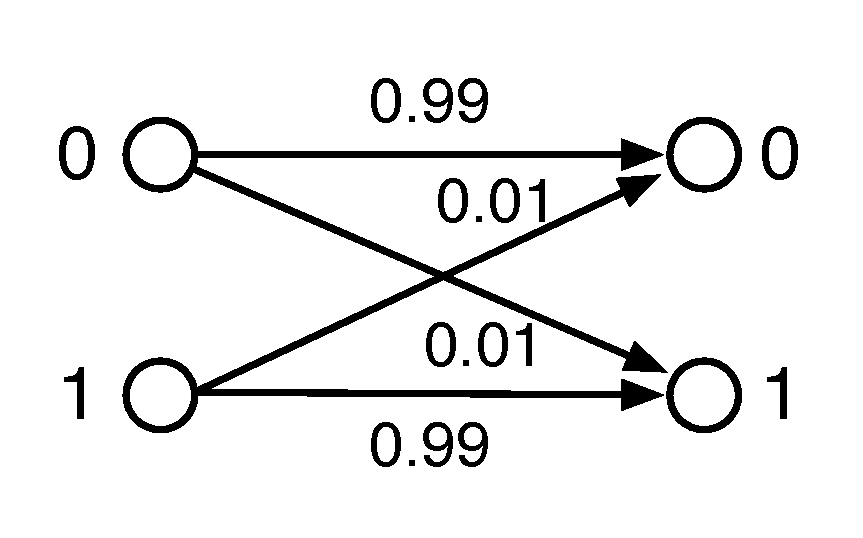
\includegraphics[width=0.4\textwidth]{img/bsc99.pdf}
\caption{BSC con p=0.01}
\label{fig:bsc99}
\end{center}
\end{figure}


Consideriamo un canale BSC con p=0.01 (figura \ref{fig:bsc99}) e supponiamo di non conoscere la sorgente, ovvero P(x). La regola di decisione 
sarà dunque quella della massima verosimiglianza. Ovvero:
\[
 d(0)=0 \\ d(1)=1
\]
Calcoliamo quindi la probabilità di errore, con la formula \eqref{perr}:
\[
 P_E=\frac{0.01+0.01}{2}=0.01
\]

Proviamo ora a migliorare l'affidabilità. In maniera abbastanza banale, inseriamo un codificatore che invia 3 volte il bit (invece di una sola). In sostanza quindi stiamo considerando l'estensione terza di un BSC. La situazione è quella rappresentata in figura \ref{fig:bsc3}. I simboli che possono essere inviati sul canale sono solamente due (000 e 111), mentre possono essere ricevute tutte le 
combinazioni di 3 bit (a seguito degli errori di trasmissione).

\begin{figure}[htbp]
\begin{center}
	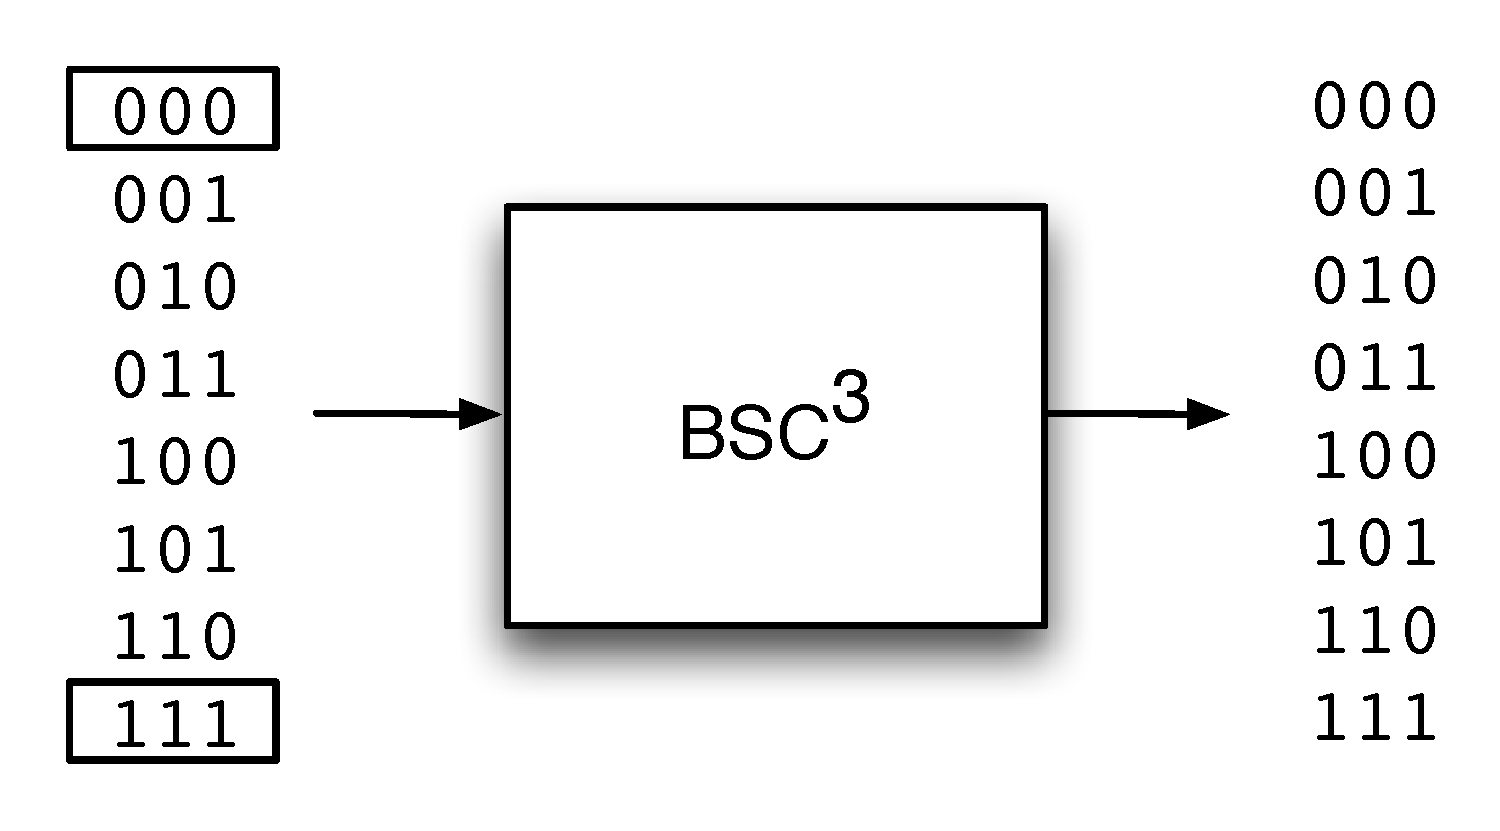
\includegraphics[width=0.6\textwidth]{img/bsc3.pdf}
\caption{$BSC^3$ con due possibili ingressi}
\label{fig:bsc3}
\end{center}
\end{figure}

La regola di decisione è abbastanza semplice. Si sceglie 0 se sono stati ricevuti più 0 che 1, mentre 1 nell'altro caso.
Poiché abbiamo scelto un'estensione dispari del canale, non ci troveremo mai nel caso in cui il numero di 0 e di 1 sia lo stesso.
Calcoliamo quindi la probabilità di errore in questo caso. Si ha un errore quando ci sono 2 o 3 bit errati. Se infatti è sbagliato 
un unico bit, si riesce banalmente a determinare il simbolo corretto. Quindi:
\[
 P_E=P(\sharp E=2)+P(\sharp E=3)
\]
Poiché la probabilità che un bit venga trasmesso in maniera non corretta è uguale a p=0.01 per tutti i simboli, si può utilizzare 
la distribuzione binomiale. Risulta quindi:
\[\begin{split}
 P_E&=p^2(1-p)^1 \binom{3}{2} + p^3(1-p)^0 \binom{3}{3} \\
    &=3p^2(1-p) +p^3 \\
    &=3 \cdot 0.01^2 \cdot 0.99 + 0.01^3 \\
    &\simeq 3 \cdot 10^{-4}
  \end{split}
\]
L'affidabilità è quindi aumentata rispetto al caso precedente. Tuttavia anche il numero di bit è aumentato, di ben 3 volte.
Possiamo quindi dire che la velocità di trasmissione (transmission rate) è 1/3. Si può procedere con l'approccio della ripetizione, aumentando il numero n di bit (sempre dispari però per quanto detto prima).

\begin{table}[htbp]
  \begin{center}
   \begin{tabular}{c | r | c}
        n & $P_E$ & Tras. Rate \\
        \hline
	1 & $10^{-2}$ & 1 \\
        3 & $3 \cdot 10^{-4}$ & 1/3 \\
        5 & $10^{-5}$ & 1/5 \\
        7 & $4 \cdot 10^{-7}$ & 1/7 \\
        9 & $10^{-8}$ & 1/9 \\
       11 & $5 \cdot 10^{-10}$ & 1/11 \\
    \end{tabular}
  \end{center}
\caption{Probabilità di errore e transmission rate, al crescere del numero di bit}
\label{tab:bscc}
\end{table}

I risultati sono quelli riportati in tabella \ref{tab:bscc}. Come si nota pare ci sia un trade-off importante: all'aumentare dell'affidabilità diminuisce notevolmente la velocità di trasmissione.
In realtà vedremo che non è così.

Proviamo ora a considerare un approccio differente. Consideriamo il caso iniziale del BSC (quindi massima velocità e minima affidabilità). Se al posto del BSC utilizziamo un $BSC^3$ ed inviamo tutte le combinazioni di bit abbiamo esattamente la stesse caratteristiche del BSC (a parte il fatto che vengono mandati 3 bit alla volta). Se indichiamo allora con M il numero di combinazioni 
inviabili (o meglio di parole di codice), in questo caso abbiamo M=8.
La situazione è rappresentata in figura \ref{fig:mbsc1}.
Viceversa, nel caso considerato prima avevamo M=2. Potevamo infatti inviare solamente due parole di codice (000 e 111), aumentavamo 
l'affidabilità e riducevamo la velocità (anche se venivano inviati 3 bit l'informazione era un solo bit). 
La situazione è rappresentata in figura \ref{fig:mbsc2}.
E' allora interessante considerare il caso intermedio, in cui M=4: si inviano 4 parole di codice (quindi 2 bit di informazione e 1 aggiuntivo).
L'esempio è rappresentato in figura \ref{fig:mbsc3}


\begin{figure}[htbp]
\begin{center}
	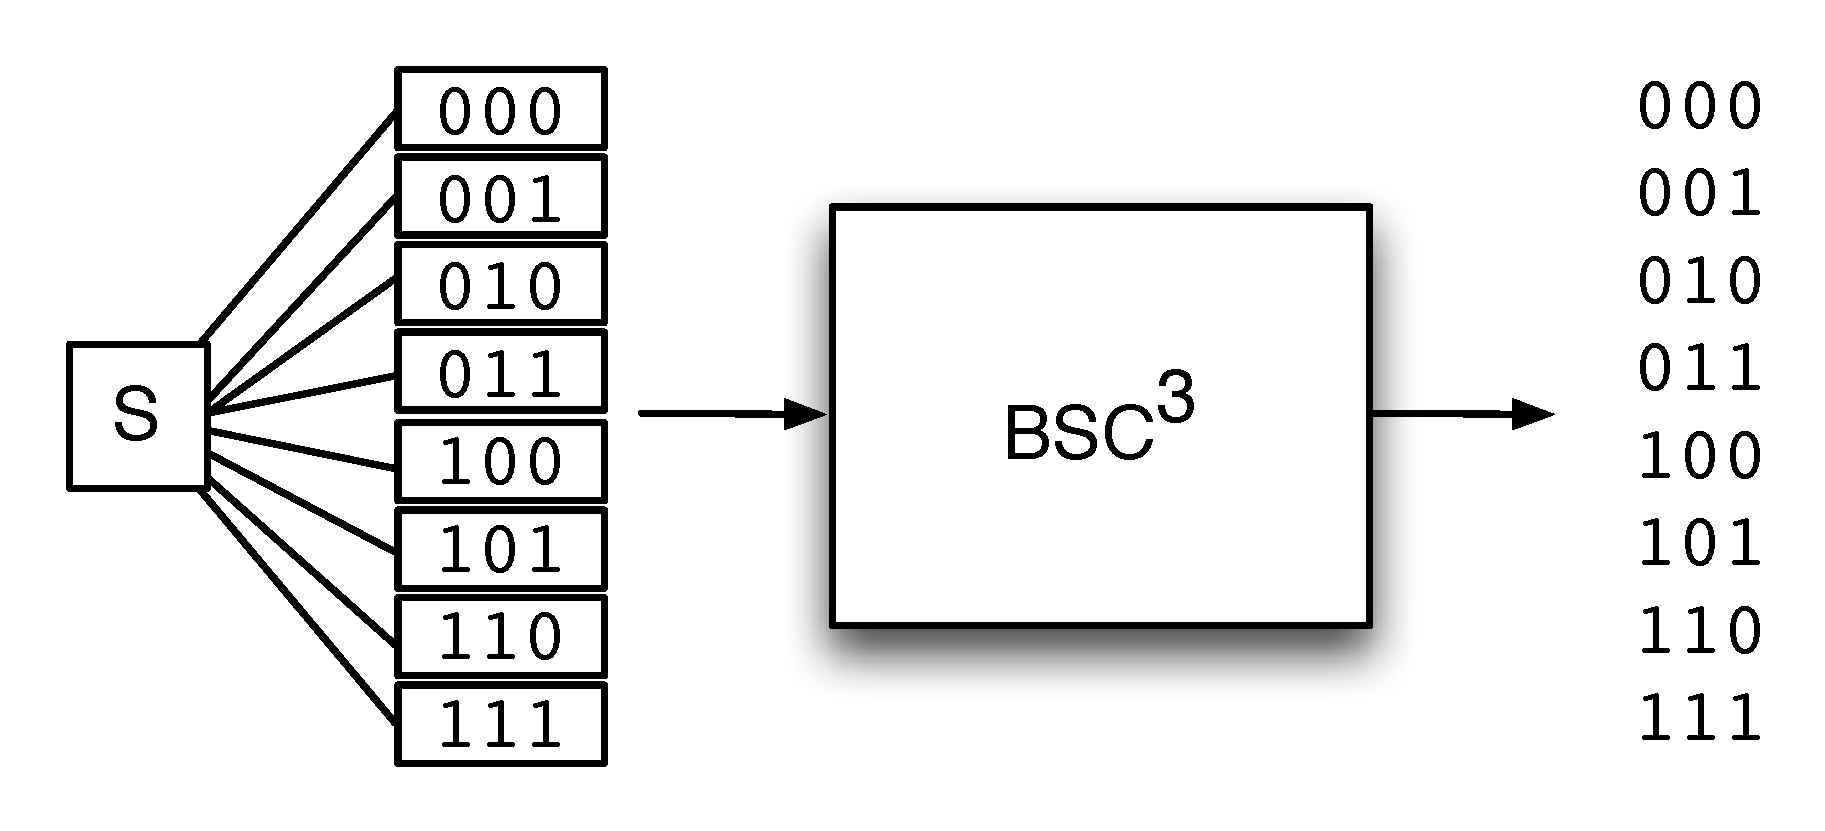
\includegraphics[width=0.6\textwidth]{img/mbsc1.pdf}
\caption{$BSC^3$ con M=8}
\label{fig:mbsc1}
\end{center}
\end{figure}

\begin{figure}[htbp]
\begin{center}
	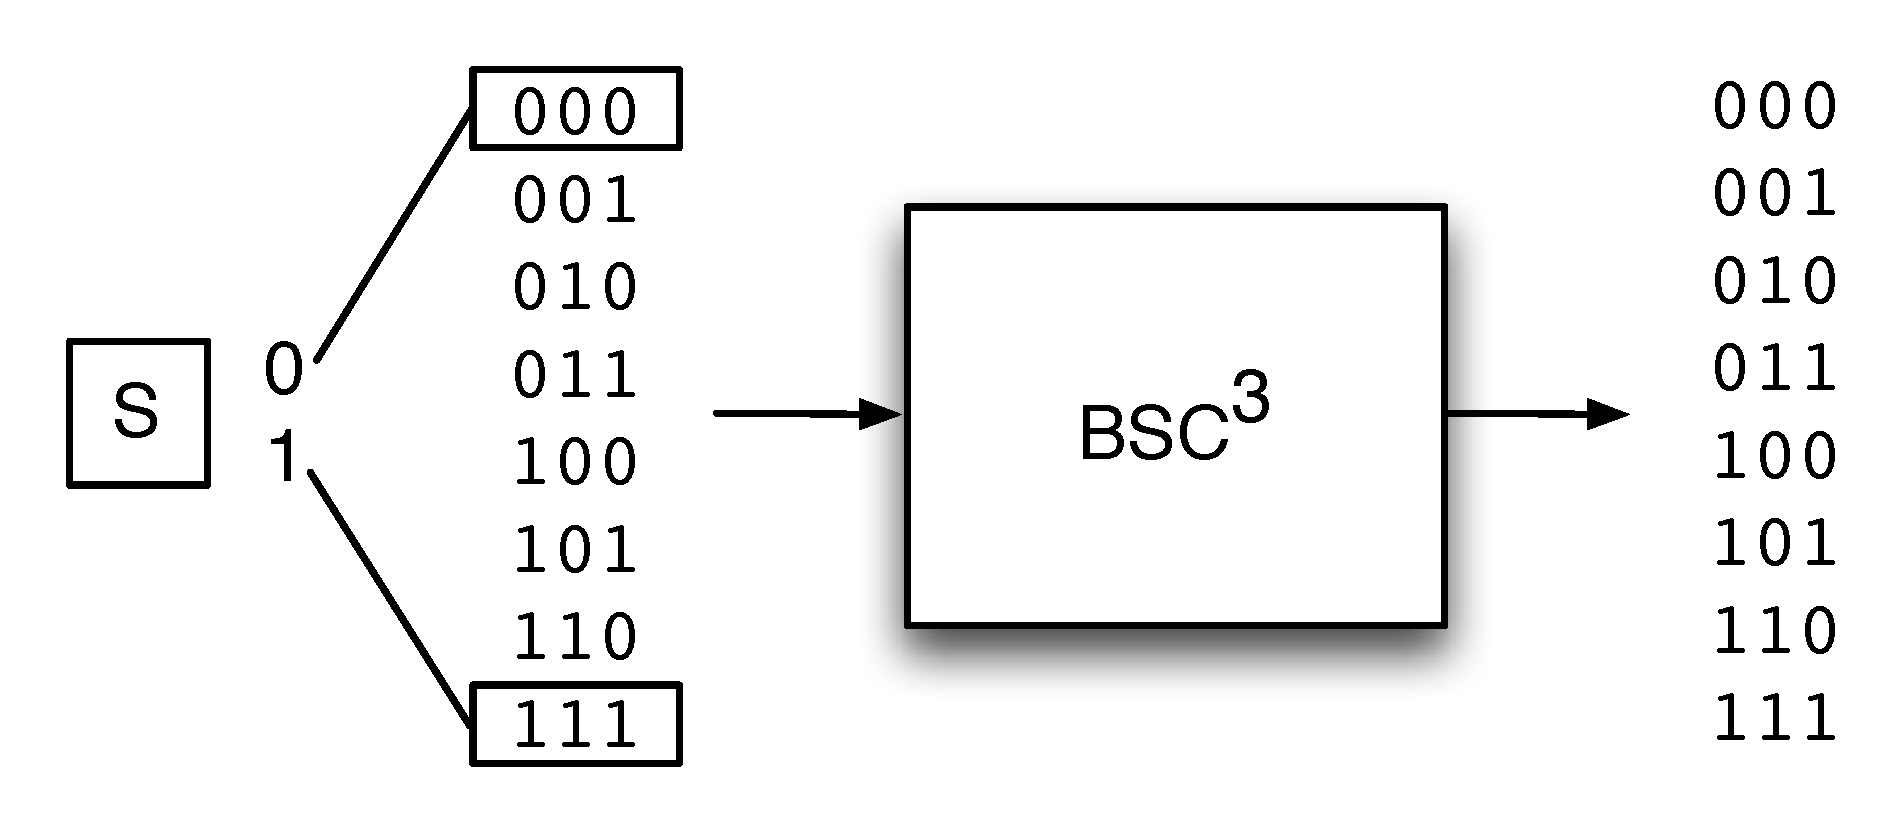
\includegraphics[width=0.6\textwidth]{img/mbsc2.pdf}
\caption{$BSC^3$ con M=2}
\label{fig:mbsc2}
\end{center}
\end{figure}

\begin{figure}[htbp]
\begin{center}
	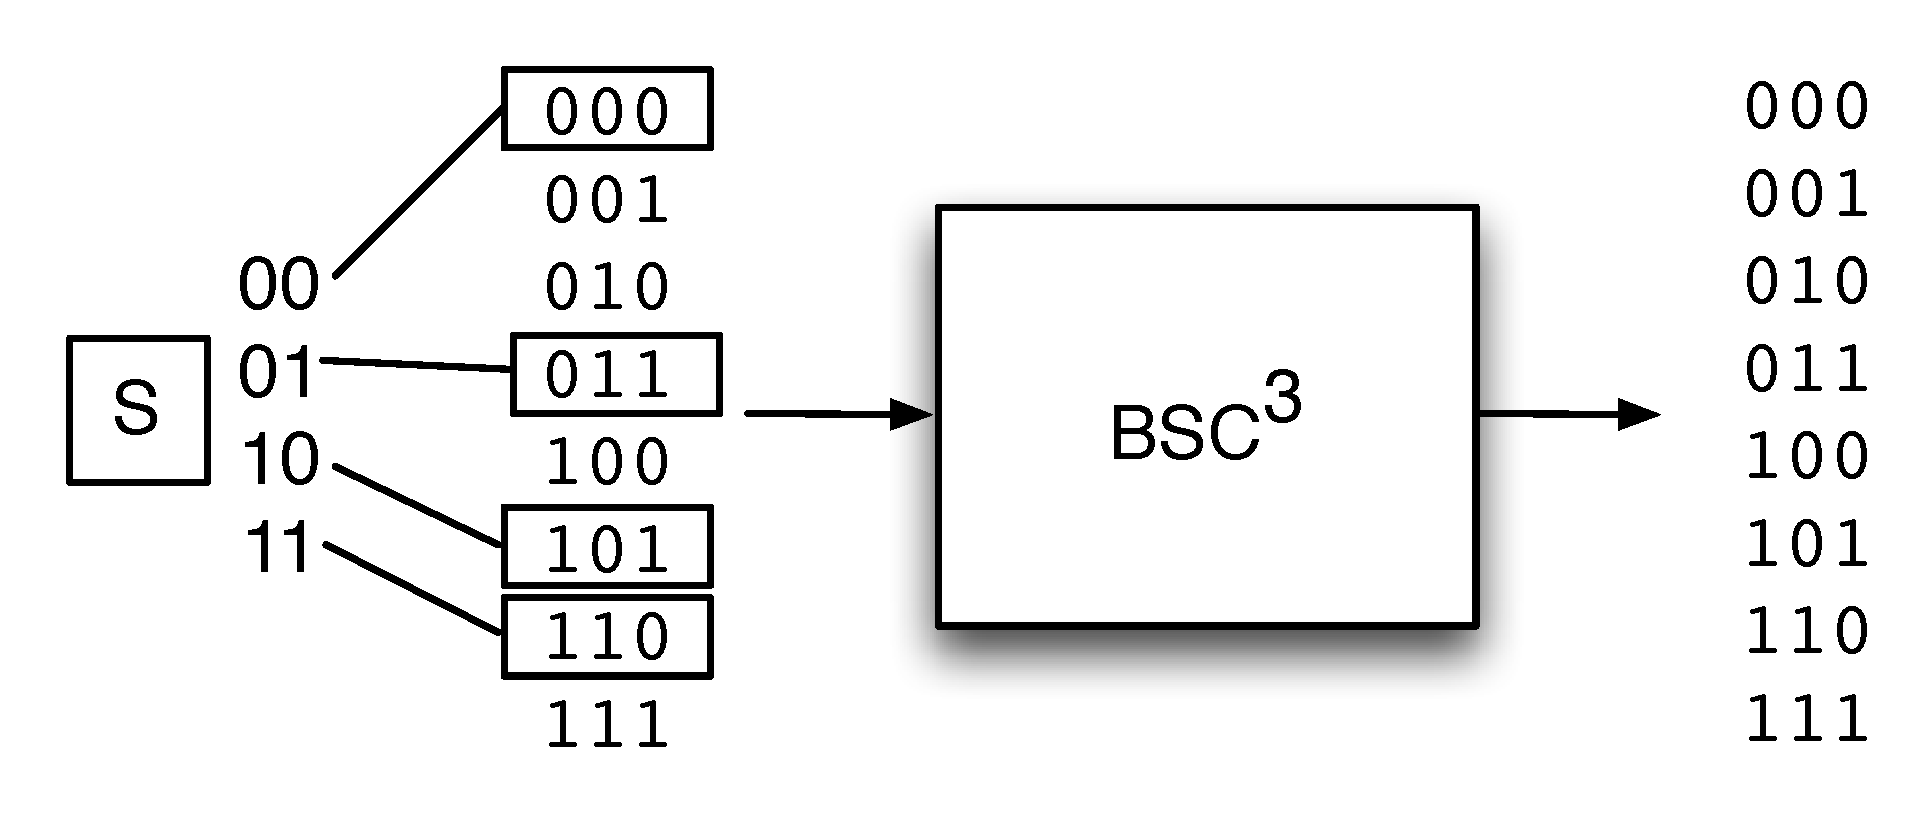
\includegraphics[width=0.6\textwidth]{img/mbsc3.pdf}
\caption{$BSC^3$ con M=4}
\label{fig:mbsc3}
\end{center}
\end{figure}

\newpage
\noindent
La funzione di decodifica per quest'ultimo caso è la seguente:
\[\begin{split}
 &d(000)=d(001)=00  \\
 &d(010)=d(011)=01  \\
 &d(100)=d(101)=10  \\
 &d(110)=d(111)=11  \\
 \end{split}
\]
Per scegliere i simboli da inviare sul canale, si può utilizzare il concetto di distanza di Hamming:
\begin{definizione}[Distanza di Hamming]
La distanza di Hamming tra due parole di codice (di uguale lunghezza) è il numero di posizioni in cui i 
simboli delle due parole differiscono.
\end{definizione}

Per esempio 000 e 011 hanno distanza di Hamming pari a 2 (gli ultimi 2 bit differiscono). Le parole di codice da inviare sono 
quindi state scelte al fine di massimizzare la distanza di Hamming tra le varie parole. Si nota infatti che la minima distanza in 
questo caso tra due parole qualsiasi è 2. In questo modo è possibile ``distanziare'' il più possibile le parole di codice, in maniera che errori sui singoli bit non transformino una parola di codice in un'altra.

%
%Confrontiamo ora la probabilità di errore e il transmission rate al variare di M nei tre casi.
%
%\begin{table}[htbp]
%  \begin{center}
%   \begin{tabular}{c | r |  c}
%        M & $P_E$ &  Tras. Rate \\
%        \hline
%	2 & $3 \cdot 10^{-4}$ & 0.33 \\
%        4 & $2 \cdot 10^{-2}$ & 0.66 \\
%        8 & $3 \cdot 10^{-2}$ & 1 \\
%    \end{tabular}
%  \end{center}
%\caption{Probabilità di errore e transmission rate, al variare di M}
%\label{tab:confrm}
%\end{table}

Variando i due parametri che abbiamo considerato finora: l'estensione n del canale e le parole di codice inviabili M possiamo ottenere moltissimi codici (detti codici (M,n)).

\begin{definizione}[Codice di canale (M,n)]
Un codice di canale (M,n) con:
\begin{itemize}
 \item n Estensione del canale
 \item M Numero di parole di codice inviabili sul canale
\end{itemize}
Si compone di:
\begin{itemize}
 \item Un index set $\{1,2,...,M\}$
 \item Una funzione di codifica $X^n: \{1,2,...,M\} \to X^n$
 \item Una regola di decisione d: $y^n \to \{1,2,...,M\}$
\end{itemize}

\end{definizione}

\begin{osservazione}
 Dato un codice (M,n) il suo transmission rate è:
\[
 R=\frac{log(M)}{n}
\]

\end{osservazione}

\section{2° Teorema di Shannon}
Supponiamo di voler inviare un insieme n tendente ad infinito, di parole di codice in un canale. Nel codice a ripetizione che abbiamo visto nel paragrafo precedente, eravamo in grado di ridurre arbitrariamente la probabilità di errore. Tuttavia avevamo visto che ciò 
portava ad una riduzione del transmission rate. Nel caso limite in cui la probabilità di errore tendeva a 0, anche la velocità di trasmissione tendeva a 0.
L'importante risultato del secondo teorema di Shannon dimostra invece che è possibile ridurre arbitrariamente la probabilità di errore, 
purché il transimission rate sia inferiore alla capacità di canale. In altre parole scelto un transmission rate a piacere (più piccolo della capacità di canale) si potrà trasmettere con una probabilità di errore tendente a 0.

Per vedere in maniera intuitiva che ciò è vero, consideriamo i risultati visti nel paragrafo relativo all'AEP (vedi par. \ref{aep}).
Supponiamo di poter inviare sul canale le parole di codice $X_1..X_M$. Per ciascuna di esse, il destinatario può ricevere qualsiasi 
sequenza di $Y^n$, tuttavia per il teorema AEP nella quasi totalità dei casi saranno ricevute solamente delle sequenze tipiche.
Possiamo quindi pensare intuitivamente per ogni parola di codice inviata, le sequenze ricevute siano solamente quelle comprese in una 
``sfera''. Il numero di sequenze in ogni sfera (sempre per l'AEP) è circa $2^{n H(Y/X)}$. Avremo quindi M sfere (una per ogni parola di codice), ciascuna con $2^{n H(Y/X)}$ sequenze. La situazione è quindi quella rappresentata in figura \ref{fig:sha2}.

\begin{figure}[htbp]
\begin{center}
	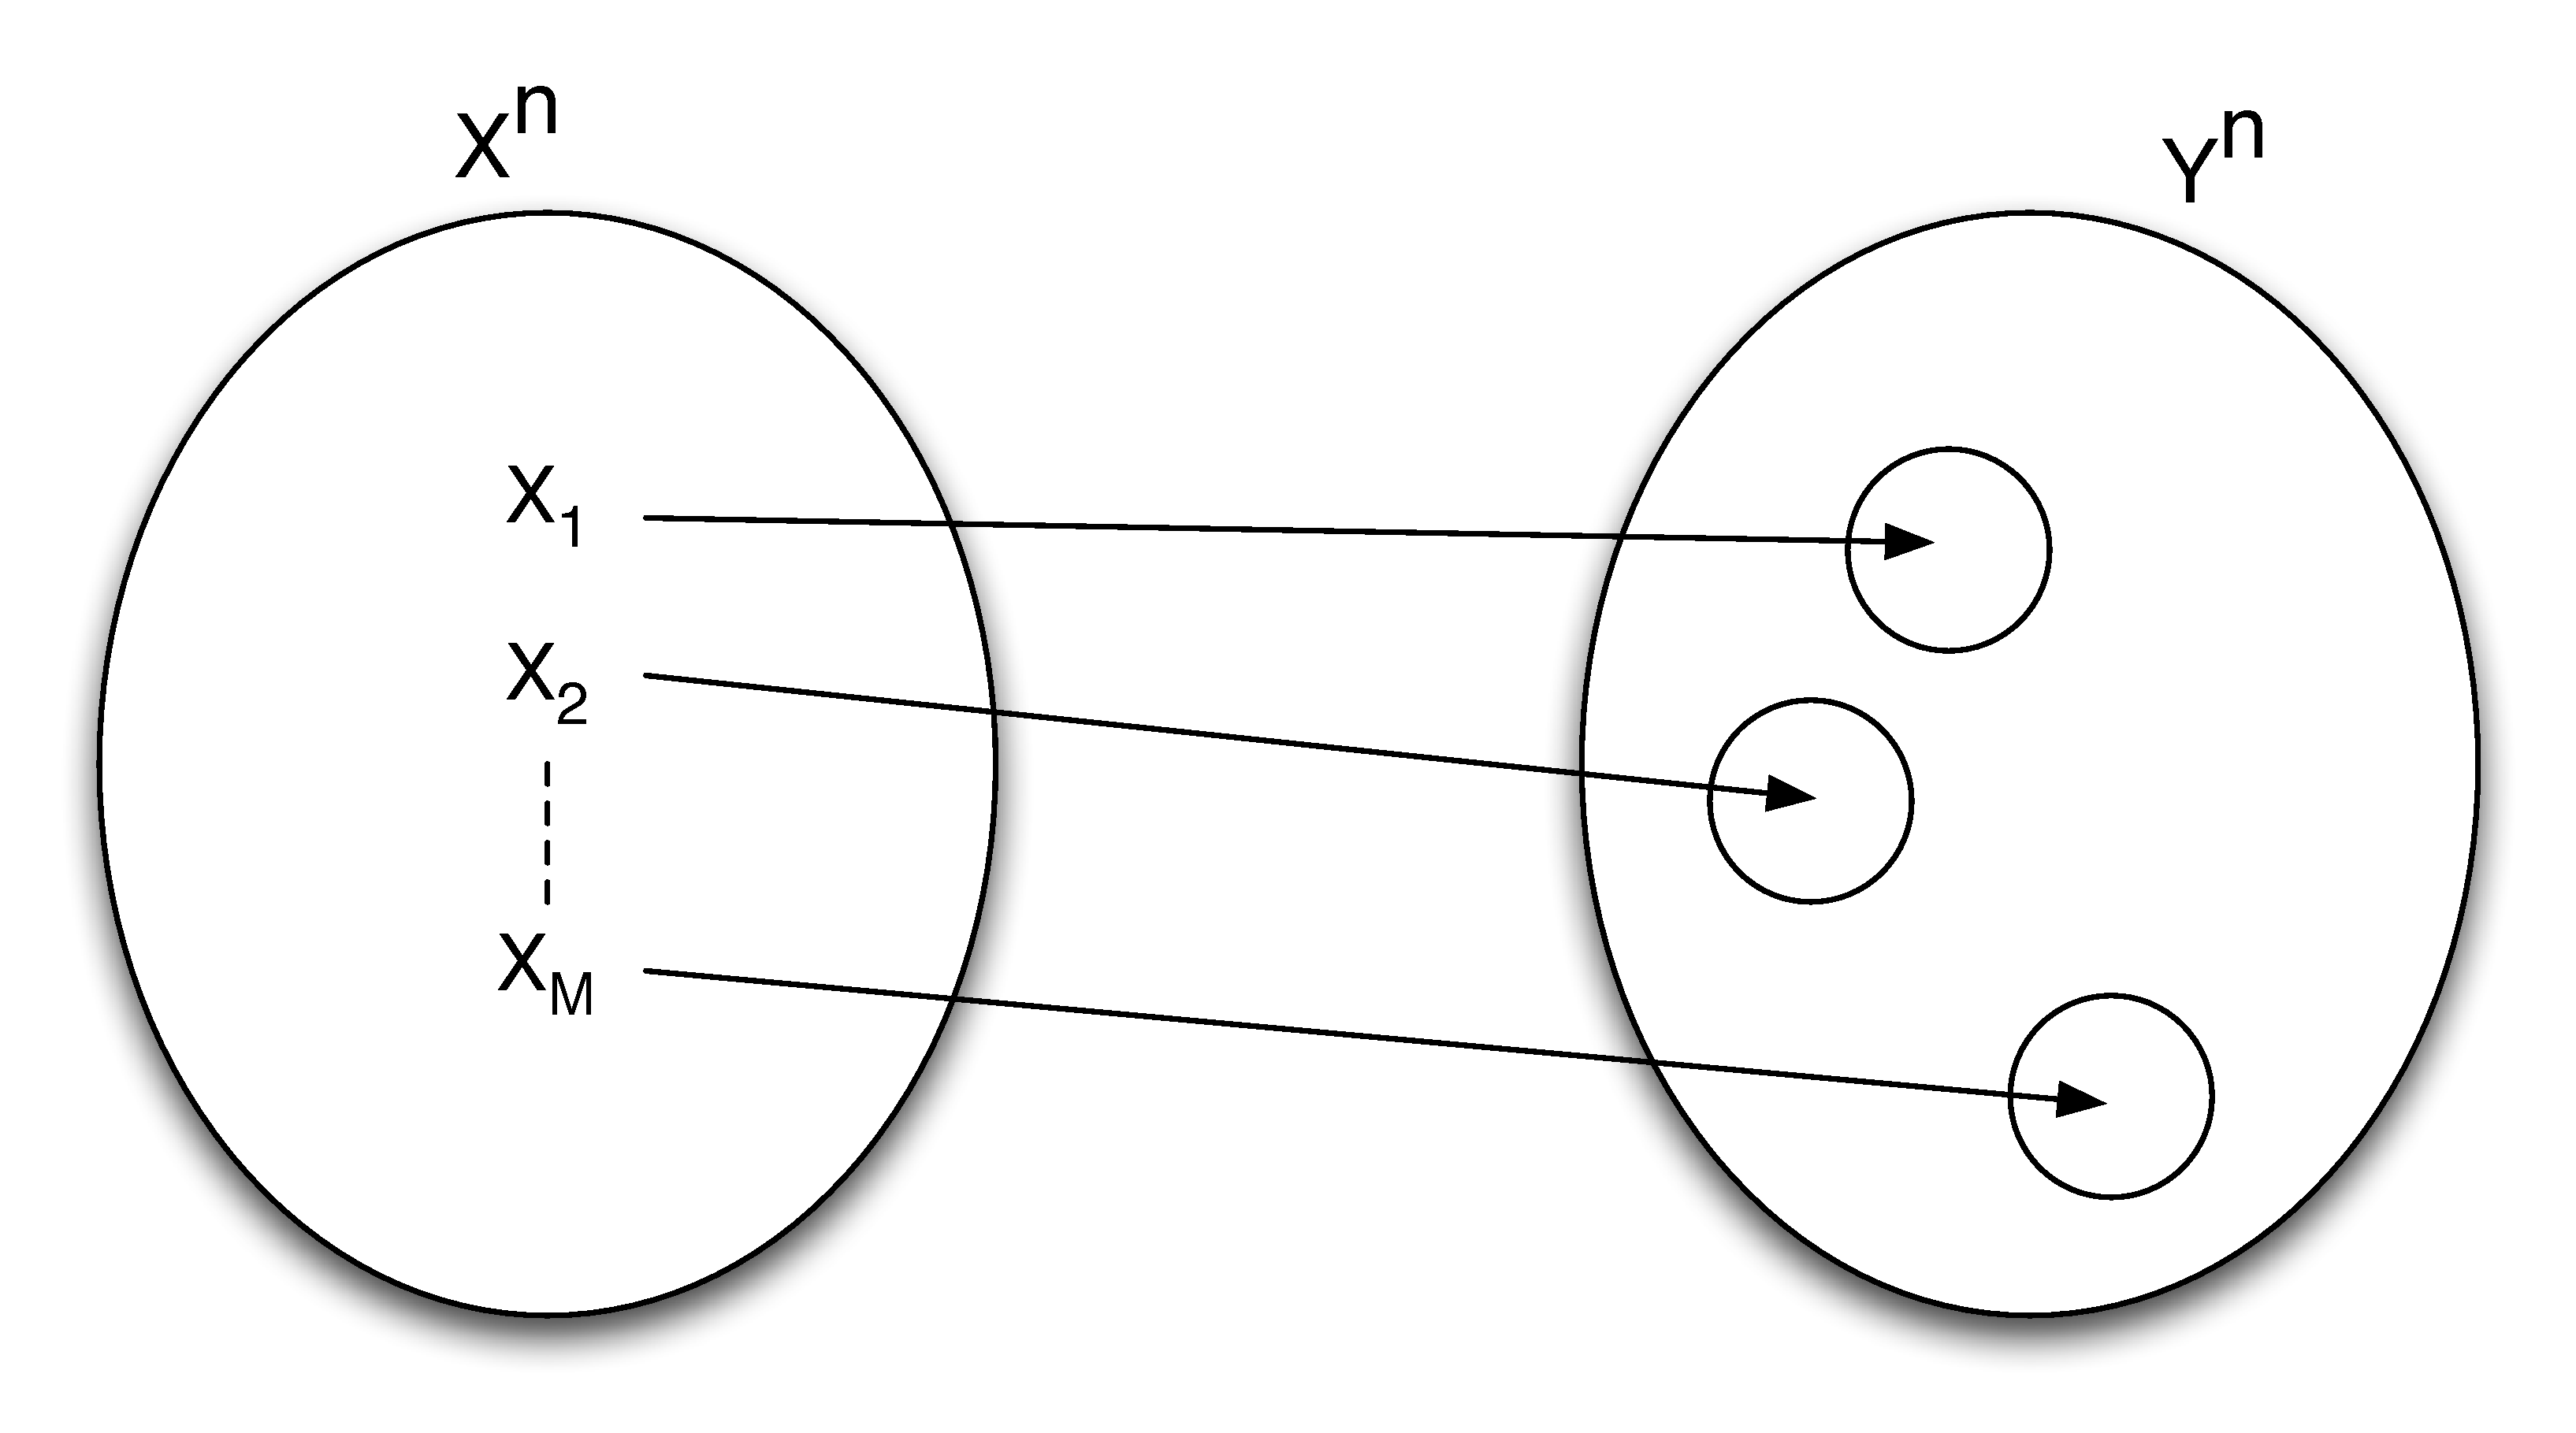
\includegraphics[width=0.6\textwidth]{img/sha2.pdf}
\caption{Rappresentazione intuitiva delle parole di codice inviate e delle sfere con le sequenze ricevute}
\label{fig:sha2}
\end{center}
\end{figure}

Si ponga ora attenzione al fatto che il numero totale di sequenze non è $M \times 2^{n H(Y/X)}$. Infatti non è detto che
le sfere siano tutte disgiunte. Il numero totale di sequenze tipiche è invece circa $2^{n H(Y)}$ (sempre per l'AEP). 
Ma sapendo quante sequenze contiene ogni sfera, possiamo ricavare il numero massimo di sfere possibili, affinché esse non si intersichino:
\[\begin{split}
 n_{max}&=\frac{2^{n H(Y)}}{2^{n H(Y/X)}} \\
    &=2^{n (H(Y)-H(Y/X))} \\
    &=2^{n I(X;Y) }
  \end{split}
\]

Ma per avere una trasmissione affidabile, siamo proprio interessati al fatto che non ci sia intersezione tra le sfere. In caso contrario infatti per una sequenza che fa parte di due sfere, si avrebbero più parole di codice possibili tra cui scegliere. Il numero M di sfere, deve essere quini inferiore ad $n_{max}$, per essere in grado di determinare la parola 
di codice inviata.
Deve quindi essere:
\[\begin{split}
 M \le & 2^{n I(X;Y)} \\
  log(M) \le & n I(X;Y) \\
 \frac{log(M)}{n} \le & I(X;Y) \\
 R \le & I(X;Y) \\
 R \le & I(X;Y) \le C \\
 R \le & C \\
  \end{split}
\]

\bigskip

Passiamo ora alla formulazione e dimostrazione vera e propria del teorema. Al solito, presentiamo prima alcuni risultati utili per la dimostrazione. Innanzitutto introduciamo il concetto di canali in cascata. Dati due canali $C_1$ e $C_2$, possiamo infatti porli appunto ``in cascata'', ovvero uno di seguito all'altro. La situazione è quella rappresentata in figura \ref{fig:cascata}. E' possibile indicare (riferendoci ai simboli usati in figura) che i canali sono in cascata con $X \to Y \to Z$.

\begin{figure}[htbp]
\begin{center}
	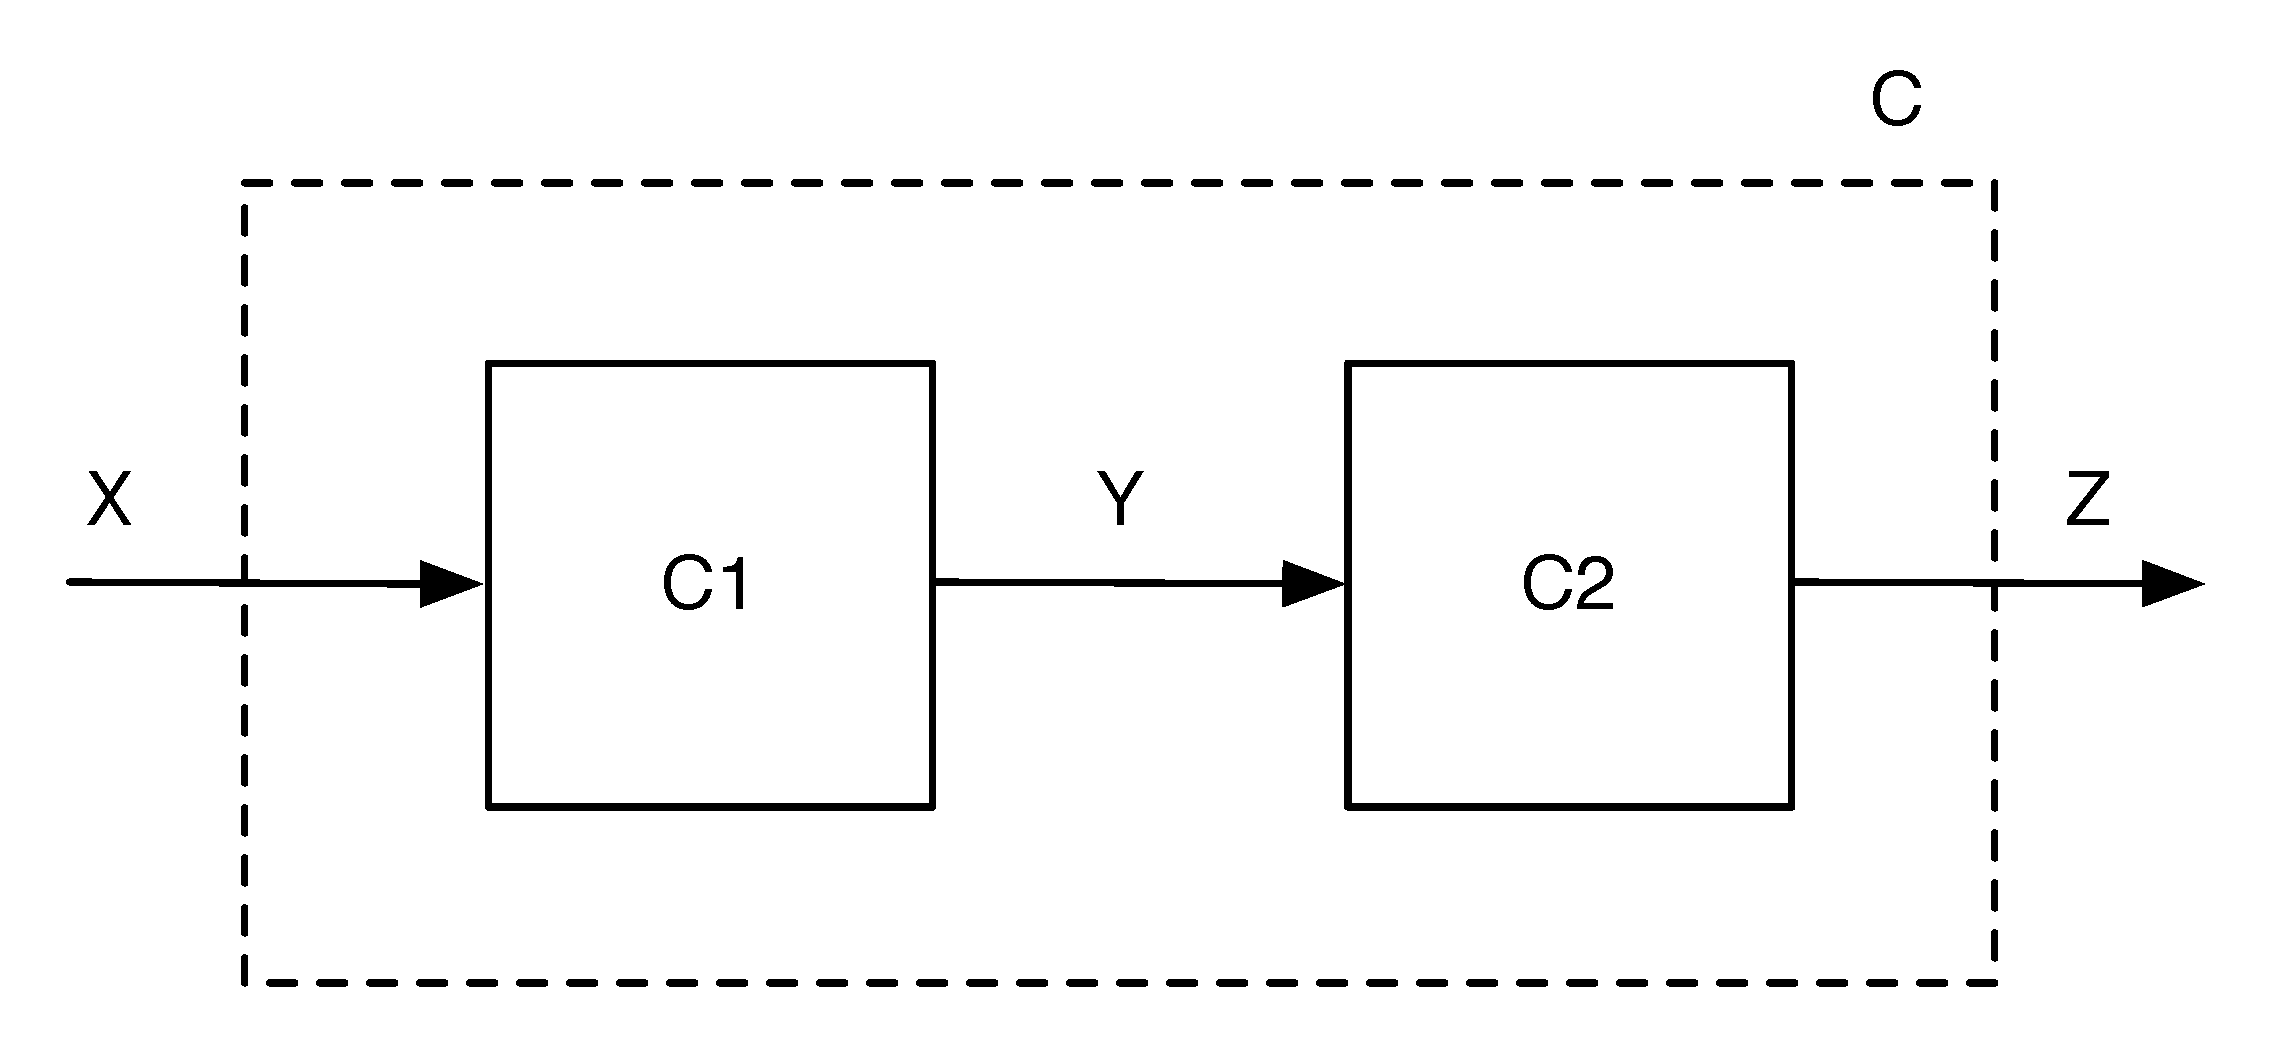
\includegraphics[width=0.6\textwidth]{img/cascata.pdf}
\caption{Due canali in cascata}
\label{fig:cascata}
\end{center}
\end{figure}

E' interessante determinare la matrice di canale che si ottiene ponendo in cascata due canali $C_1$ e $C_2$. In maniera abbastanza semplice, si nota come tale matrice è il prodotto delle matrici di canale di $C_1$ e $C_2$, ovvero $P=P_1 \times P_2$. Per fare un esempio consideriamo due canali BSC, rispettivamente con matrici di canale P1 e P2:

\[ P_1 = \left[
  \begin{array}{cc}
    1-p_1 & p_1 \\
    p_1 & 1-p_1 \\
  \end{array} \right]
  \\
  P_2 = \left[
  \begin{array}{cc}
    1-p_2 & p_2 \\
    p_2 & 1-p_2 \\
  \end{array} \right]
\]

Allora la matrice P, del canale che si ottiene ponendoli in cascata è:
\[
 P = \left[
  \begin{array}{cc}
    (1-p_1)(1-p_2) + p_1 p_2 & (1-p_1)p_2 + p_1(1-p_2) \\
    p_1 (1-p_2)+(1-p_1)p_2 & p_1 p_2 +(1-p_1)(1-p_2)\\
  \end{array} \right]
\]

\begin{figure}[htbp]
\begin{center}
	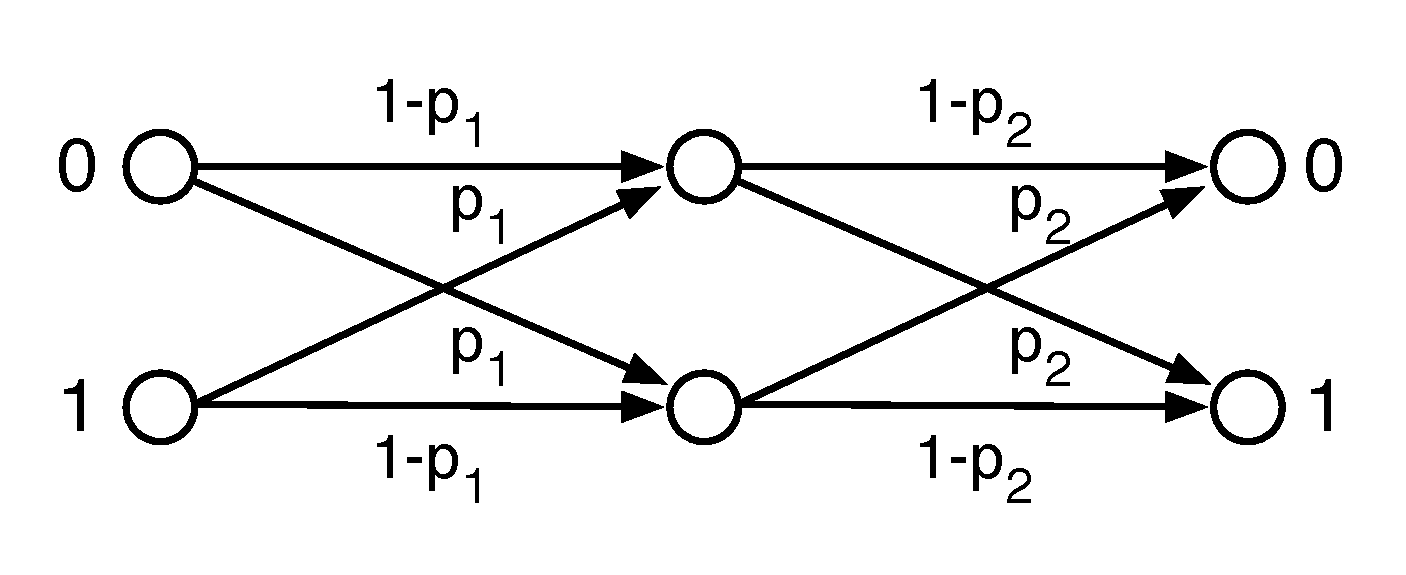
\includegraphics[width=0.6\textwidth]{img/cascata2.pdf}
\caption{Due BSC in cascata}
\label{fig:cascata2}
\end{center}
\end{figure}

\bigskip



\begin{lemma}
\mbox{}

Dati due canali in cascata $X \to Y \to Z$:
 \begin{itemize}
  \item $p(z/y,x)=p(z/y)$
  \item $p(x/y,z)=p(x/y)$
 \end{itemize}
 \begin{proof}
  Dimostriamo solo la seconda uguaglianza:
  \[\begin{split}
   p(x/y,z)=& \frac{p(y,z/x)p(x)}{p(y,z)} \\
   =&\frac{p(z/x,y)p(y/x)p(x)}{p(z/y)p(y)} \\
   =&\frac{p(z/y)p(y/x)p(x)}{p(z/y)p(y)} \\
   =&\frac{p(y/x)p(x)}{p(y)} \\
   =&p(x/y)
    \end{split}
  \]

 \end{proof}
\label{lem:cascata}
\end{lemma}

\begin{teorema}[Disuguaglianza dell'elaborazione dati]
\mbox{}

Dati due canali in cascata $X \to Y \to Z$:
 \begin{itemize}
  \item $I(X;Y) \ge I(X;Z)$
  \item $I(Y;Z) \ge I(X;Z)$
 \end{itemize}
\begin{proof}
 Dimostriamo solo la prima disuguaglianza.
 \[
  I(X;Y)=H(X)-H(X/Y)
 \]
 E:
 \[
  I(X;Z)=H(X)-H(X/Z)
 \]
 Quindi dimostrare che $I(X;Y) \ge I(X;Z)$, equivale a dimostrare che:
 \[\begin{split}
  & H(X)-H(X/Y) \ge H(X)-H(X/Z) \\
  \iff & -H(X/Y) \ge -H(X/Z) \\
  \iff & H(X/Y) \le H(X/Z) \\
  \iff & H(X/Y)-H(X/Z) \le 0 \\
  \iff & H(X/Z)-H(X/Y) \ge 0 \\
   \end{split}
 \]
Ora:
\[\begin{split}
  & H(X/Z)-H(X/Y)= \\
 =&\sum_{x \in X} \sum_{z \in Z} p(x,z) log \frac{1}{p(x/z)} - \sum_{x \in X} \sum_{y \in Y} p(x,y) log \frac{1}{p(x/y)} \\
 =&\sum_{x \in X} \sum_{z \in Z} log \frac{1}{p(x/z)}  \sum_{y \in Y} p(x,y,z) 
  - \sum_{x \in X} \sum_{y \in Y} log \frac{1}{p(x/y)} \sum_{z \in Z} p(x,y,z) \\
 =&\sum_{x \in X} \sum_{y \in Y} \sum_{z \in Z} p(x,y,z) log \frac{1}{p(x/z)} 
  - \sum_{x \in X} \sum_{y \in Y} \sum_{z \in Z} p(x,y,z) log \frac{1}{p(x/y)} \\
 =&\sum_{x \in X} \sum_{y \in Y} \sum_{z \in Z} p(x,y,z) log \frac{p(x/y)}{p(x/z)} \\
  \end{split}
\]
Ma per il lemma \ref{lem:cascata} $p(x/y)=p(x/y,z)$, quindi:
\[\begin{split}
  &\sum_{x \in X} \sum_{y \in Y} \sum_{z \in Z} p(x,y,z) log \frac{p(x/y)}{p(x/z)} \\
 =&\sum_{x \in X} \sum_{y \in Y} \sum_{z \in Z} p(x,y,z) log \frac{p(x/y,z)}{p(x/z)} \\
 =&\sum_{x \in X} \sum_{y \in Y} \sum_{z \in Z} p(y,z) p(x/y,z) log \frac{p(x/y,z)}{p(x/z)} \\
 =&\sum_{y \in Y} \sum_{z \in Z} p(y,z) \sum_{x \in X} p(x/y,z) log \frac{p(x/y,z)}{p(x/z)} \\
 \ge & 0
 \end{split}
\]
L'ultimo passaggio deriva dal fatto che $p(y,z)$ è una probabilità (e quindi maggiore uguale a 0), mentre il 
secondo termine è una distanza di Kullback-Leibler, che per il teorema \ref{leibler} è maggiore o uguale a 0.
\end{proof}
\end{teorema}

\medskip

La disuguaglianza dell'elaborazione dati dice in sostanza che l'informazione mutua, man mano che si attraversano dei canali, 
non può aumentare. In sostanza ad ogni ``passaggio'' si può solo perdere informazione (e mai guadagnarne).

\bigskip

\begin{teorema}[Disuguaglianza di Fano]
\mbox{}

Siano X,Y variabili casuali e $g(Y)=\widehat{X}$ una regola di decisione. Sia:
\[
 P_E=P\{\widehat{X} \neq X\}
\]
Allora:
\[
 H(X/Y) \le H(P_E)+P_E log(|X|-1)
\]
\begin{proof}
\mbox{}

 Costruiamo una nuova variabile casuale E, nel seguente modo:
 \[
  E=
  \begin{cases}
    1 & \widehat{X} \neq X \\
    0 & \widehat{X}=X \\
  \end{cases}
 \]
 Allora:
 \[\begin{split}
   H(X/Y)=&H(X/Y)+H(E/X,Y) \\
         =&H(E,X/Y) \\
         =&H(E/Y)+H(X/E,Y) \\
         \le & H(E) + H(X/E,Y) \\
         = & H(P_E) + H(X/E,Y) \\
   \end{split}
 \]

Il primo passaggio deriva dal fatto che $H(E/X,Y)=0$ in quanto se si conoscono X e Y, allora banalmente si conosce anche E. 
Il secondo e il terzo sono applicazioni 
della regola della catena (in particolare corollario del teorema \ref{catena}). Il quarto passaggio 
deriva dal fatto che il condizionamento riduce l'entropia (osservazione \ref{condizionamento}).
Ora:
\[\begin{split}
 H(X/E,Y) =&Pr\{E=0\}H(X/Y,E=0)+
           Pr\{E=1\}H(X/Y,E=1) \\
          =&Pr\{E=0\} \cdot 0 + Pr\{E=1\}H(X/Y,E=1) \\
          =&Pr\{E=1\}H(X/Y,E=1) \\
          =&P_E H(X/Y,E=1) \\
          \le& P_E log(|X|-1)
  \end{split}
\]
L'ultimo passaggio deriva dal fatto che il massimo valore che può raggiungere l'entropia è il logaritmo del 
numero di simboli. Ma se E=1 allora $\widehat{X}\neq X$, quindi ho qualche informazione in più sul simbolo inviato. 
Ovvero so che non sarà $\widehat{X}$. Rimane dunque da ``scegliere'' tra $|X|-1$ simboli, la cui massima entropia è proprio 
$log(|X|-1)$.
Riassumendo:
\[
 H(X/Y) \le H(P_E) + H(X/E,Y) \le H(P_E)+P_E log(|X|-1)
\]
Che conclude la dimostrazione
\end{proof}
\end{teorema}

\begin{corollario}
 \[
  H(X/Y) \le 1+P_E log(|X|)
 \]
\begin{proof}
 Segue direttamente dal teorema:
 \[\begin{split}
 H(X/Y) & \le H(P_E)+P_E log(|X|-1) \\
        & \le log(2) + P_E log(|X|-1) \\
        & \le 1 + P_E log(|X|)
  \end{split}
 \]
\end{proof}
\end{corollario}


\begin{lemma}
 Sia $C=(X,p(y/x),Y)$ un canale senza memoria e sia 
$C^n=(X^n,p^n(x,y),Y^n)$ la sua estensione n-esima. Allora:
\[
 I(X^n;Y^n) \le nC
\]
\begin{proof}
 \mbox{}
Ricordando che se C è senza memoria:
\[
p(y^n/x^n)=\prod_{i=1}^n p(y_i,x_i) 
\]
Si ha:
\[\begin{split}
 I(X^n;Y^n) &=H(Y^n)-H(Y^n/X^n) \\
 & = \sum_{i=1}^n H(Y_i/Y_1,Y_2,...,Y_{i-1}) - H(Y^n/X^n) \\
 & \le \sum_{i=1}^n H(Y_i) - H(Y^n/X^n) \\
 & \le \sum_{i=1}^n H(Y_i) - \sum_{i=1}^n H(Y_i/Y_1,Y_2,...,Y_{i-1},X^n) \\
 & = \sum_{i=1}^n H(Y_i) - \sum_{i=1}^n H(Y_i/X_i) \\
 & = \sum_{i=1}^n  [ \ H(Y_i)- H(Y_i/X_i) \  ] \\
 & = \sum_{i=1}^n I(X_i;Y_i) \\
 & \le nC
  \end{split}
\]
\end{proof}
Il secondo e il quarto passaggio seguono dalla regola della catena (generalizzata).
Il terzo passaggio segue invece dal fatto che il condizionamento riduce l'entropia (oss. \ref{condizionamento}).
Il quinto passaggio deriva dal fatto che il canale è senza memoria.
L'ultimo passaggio, infine, deriva dal fatto che la capacità di canale è il massimo dell'informazione mutua.
\label{lsh}
\end{lemma}


\bigskip

\noindent
Possiamo ora enunciare e dimostrare una parte del 2° teorema di Shannon.

\begin{teorema}[2° teorema di Shannon (o della codifica di canale)]
 \mbox{}

 \begin{enumerate}
  \item Sia $A=(X,p(y/x),Y)$ un canale con capacità C e sia $R \le C$.

        \noindent
        Allora esiste una sequenza di codici $(2^{nR},n)$ tali che:
        \[
         P_E^{(n)} \xrightarrow[n \to \infty]{} 0
        \]
        Ovvero:
        \[
         \forall \epsilon>0, \exists n_0 \in N: \forall n \ge n_0 \ P_E^{(n)}< \epsilon
        \]
   \item Se esiste una sequenza di codici $(2^{nR},n)$, tali che:
         \[
          P_E^{(n)} \xrightarrow[n \to \infty]{} 0
         \]
         Allora $R \le C$
 \end{enumerate}
 \begin{proof}
  \mbox{}
  \begin{description}
   \item[1.] Omesso, la dimostrazione è complicata.
   \item[2.] 
    
    Indichiamo con W l'insieme delle parole di codice inviabili sul canale.
    Quindi:
    \[
     W \to X^n(W) \to Y^n
    \]
    \noindent
    Poiché stiamo considerando dei codici $(2^{nR},n)$, si avrà:
    \[
     |W|=2^{nR}
    \]
    Quindi, poiché consideriamo le parole di codice tutte equiprobabili, si avrà:
    \[
     H(W)=log(|W|)=log(2^{nR})=nR
    \]
   Da cui:
   \[\begin{split}
    nR=H(W)&=H(W/Y^n)+I(W;Y^n) \\
        & \le H(W/Y^n)+I(X^n;Y^n) \\
        & \le H(W/Y^n)+nC \\
        & \le 1+P_E^{(n)} log(|W|) +nC \\
        & = 1+P_E^{(n)} nR +nC \\
     \end{split}
   \]
   Il secondo passaggio deriva dalla disuguaglianza dell'elaborazione dati, il terzo invece dal lemma \ref{lsh}.
   Il quarto passaggio segue dal corollario alla disuguaglianza di Fano.

   Ora dividendo ambo i membri per n si ottiene:
   \[
    R \le \frac{1}{n}+P_E^{(n)} R +C
   \]
   Ma:
   \[
    \lim_{n \to \infty} \frac{1}{n}+P_E^{(n)} R +C=C
   \]
   Da cui:
   \[
    R \le C
   \]

  \end{description}

 \end{proof}

\end{teorema}

\appendix
\chapter{Esercizi Svolti}

\textbf{Codifica di sorgente}

\begin{enumerate}
 \item Determinare se il codice con le seguenti parole è univocamente decodificabile o meno: 
       012, 0123, 4, 310, 1024, 2402, 2401, 4013.
       \bigskip
       \bigskip

       \textit{Soluzione:}

       \noindent
       Si può utilizzare l'algoritmo di Sardinas-Patterson. Risulta:
       \begin{table}[htbp]
       \begin{center}
       \begin{tabular}{l | l | l | l | l | l | l | l | l | l | l | l}
        $S_0$ & $S_1$  & $S_2$ & $S_3$ & $S_4$ & $S_5$ & $S_6$ & $S_7$ & $S_8$ & $S_9$ & $S_{10}$\\
        \hline
        012  & 3   & 10 & 24 & 02 & 2  & 402 & 3  & 10 & 24  & 3 \\
        0123 & 013 &    &    & 01 & 23 & 401 & 01 & 2  & 402 & 01 \\
        4    &     &    &    &    &    &     & 02 & 23 & 401 & 02 \\
        310  &     &    &    &    &    &     &    &    &    & \\
        1024 &     &    &    &    &    &     &    &    &    & \\
        2402 &     &    &    &    &    &     &    &    &    & \\
        2401 &     &    &    &    &    &     &    &    &    & \\
        4013 &     &    &    &    &    &     &    &    &    & \\
       \end{tabular}
       \end{center}
       \end{table}

       Il codice è dunque UD, poiché $S_{10}$ coincide con $S_7$.

       \bigskip
 \item Si costruisca un codice di Shannon binario, per la seguente varabile aleatoria:
       \[ X = \left(
        \begin{array}{cccccccc}
           x_1  & x_2  & x_3  & x_4  & x_5  & x_6  & x_7  & x_8 \\
           0.22 & 0.02 & 0.20 & 0.18 & 0.05 & 0.08 & 0.15 & 0.10 \\
        \end{array} \right)
       \]
       Si stabilisca se la lunghezza media del codice ottenuto coincide con l'entropia di X (in base 2) senza calcolare 
       né l'una né l'altra.
       \bigskip
       \bigskip

       \textit{Soluzione:}

       \noindent
       Calcoliamo le lunghezze delle varie parole di codice, per il codice di Shannon. Deve essere:
       \[
        l_i=\left \lceil -log p_i \right \rceil
       \]
       Le lunghezze sono dunque:
       \[ L = \left(
        \begin{array}{cccccccc}
           x_1  & x_2  & x_3  & x_4  & x_5  & x_6  & x_7  & x_8 \\
           3    & 6    & 3    & 3    & 5    & 4    & 3    & 4 \\
        \end{array} \right)
       \]
       Un codice con queste lunghezze è ad esempio:
       \[ C = \left(
        \begin{array}{cl}
           x_1  & \to 000 \\
           x_2  & \to 111111 \\
           x_3  & \to 011 \\
           x_4  & \to 100 \\
           x_5  & \to 11000 \\
           x_6  & \to 0101 \\
           x_7  & \to 001  \\
           x_8  & \to 1101 \\
        \end{array} \right)
       \]

       Per il teorema \ref{limitelcodice}, la lunghezza media del codice coincide con l'entropia se e solo se:
       \[
        \forall i=1..n  \ \ p_i=D^{-l_i}
       \]
       Ma non è questo il caso (ad esempio $0.22\ne2^{-3}$). La lunghezza del codice non coincide quindi con 
       l'entropia di X.
       \bigskip

 \item Si determini se i seguenti codici sono univocamente decodificabili o meno:
       \begin{itemize}
        \item $C_1=\{10,010,1,1110\}$
        \item $C_2=\{0,001,101,11\}$
        \item $C_3=\{0,2,03,011,104,341,11234\}$
       \end{itemize}
       \bigskip
       \bigskip

       \textit{Soluzione:}

       \noindent
       Si può utilizzare l'algoritmo di Sardinas-Patterson. Risulta:
       \newpage

       \begin{table}[htbp]
       \begin{center}
       \begin{tabular}{l | l | l}
        $S_0$ & $S_1$  & $S_2$ \\
        \hline
        10   & 0   & 10  \\
        010  & 110 &     \\
        1    &     &     \\
        1110 &     &     \\
       \end{tabular}
       \end{center}
       \end{table}

       Quindi $C_1$ non è UD, poiché $S_0 \cap S_2 = \{10\} \neq \varnothing $.

       \begin{table}[htbp]
       \begin{center}
       \begin{tabular}{l | l | l | l | l}
        $S_0$ & $S_1$  & $S_2$ & $S_3$ & $S_4$\\
        \hline
        0   & 01 & 1 & 1  & 1  \\
        001 &    &   & 01 & 01 \\
        101 &    &   &    &    \\
        11  &    &   &    &   \\
       \end{tabular}
       \end{center}
       \end{table}

       Quindi $C_2$ è UD, in quanto $S_3=S_4$.

       \begin{table}[htbp]
       \begin{center}
       \begin{tabular}{l | l | l | l | l | l | l | l}
        $S_0$ & $S_1$  & $S_2$ & $S_3$ & $S_4$ & $S_5$ & $S_6$ & $S_7$ \\
        \hline
        0     & 3  & 41  & 34 & 1 & 04   & 4 &\\
        2     & 11 & 234 &    &   & 1234 &   &\\
        03    &    &     &    &   &      &   &\\
        011   &    &     &    &   &      &   &\\
        104   &    &     &    &   &      &   &\\
        341   &    &     &    &   &      &   &\\
        11234 &    &     &    &   &      &   &\\
       \end{tabular}
       \end{center}
       \end{table}

       Quindi $C_3$ è UD perché $S_7=\varnothing$.

        \bigskip
\item Si costruisca un codice ottimale ternario per la seguente variabile aleatoria:
      \[ X = \left(
        \begin{array}{cccccccc}
           x_1  & x_2  & x_3  & x_4  & x_5  & x_6  & x_7  & x_8 \\
           0.22 & 0.02 & 0.20 & 0.18 & 0.05 & 0.08 & 0.15 & 0.10 \\
        \end{array} \right)
       \]
       Si stabilisca se la lunghezza media del codice ottenuto coincide con l'entropia di X (in base tre) 
       senza calcolare né l'una né l'altra.
       \bigskip
       \bigskip

       \textit{Soluzione:}

       \noindent
       Si può utilizzare l'algoritmo di Huffman. Poiché è richiesto un codice ternario, deve essere n=1 mod 2.
       E' necessario quindi aggiungere un simbolo aggiuntivo (infatti 9=4*2+1).
       Risulta:
       \begin{table}[htbp]
       \begin{center}
        \begin{tabular}{l || l|l|| l|l|| l|l|| l|l}
            &$S_0$ &$C_0$&$S_1$       & $C_1$& $S_2$        & $C_2$& $S_3$        & $C_3$ \\
       \hline
      $x_1$ & 0.22 &2  & 0.22           &2  &$\boxed{0.25}$ & 1  &$\boxed{0.53}$  & 0 \\
      $x_3$ & 0.20 &00 & 0.20           &00 &0.22           & 2  &0.25            & 1 \\
      $x_4$ & 0.18 &01 & 0.18           &01 &0.20           & 00 &0.22            & 2 \\
      $x_7$ & 0.15 &02 & 0.15           &02 &0.18           & 01 &                & \\
      $x_8$ & 0.10 &10 & 0.10           &10 &0.15           & 02 &                & \\
      $x_6$ & 0.08 &11 & 0.08           &11 &               &    &                & \\
      $x_5$ & 0.05 &120 & $\boxed{0.07}$ &12 &               &    &                & \\
      $x_2$ & 0.02 &121 &                &   &               &    &                & \\
        \hline
            & 0    &122 & & & & & &\\    
       \end{tabular}
       \end{center}
       \end{table} 

      \noindent
      Un codice ottimale è dunque:
       \[ C = \left(
        \begin{array}{cl}
           x_1  & \to 2 \\
           x_2  & \to 121 \\
           x_3  & \to 00 \\
           x_4  & \to 01 \\
           x_5  & \to 120 \\
           x_6  & \to 11 \\
           x_7  & \to 02  \\
           x_8  & \to 10 \\
        \end{array} \right)
       \]

       La lunghezza del codice non coincide con l'entropia, perché X non è 3-adica. Infatti, ad esempio, 
       $-log_3 0.22 \simeq 1.37 \neq 1 $
        \bigskip
\item E' possibile costruire un codice binario univocamente decodificabile con lunghezze di parola 2,2,3,3,3,4,4,4? 
      Giustificare la risposta.
       \bigskip
       \bigskip

       \textit{Soluzione:}

       \noindent
       E' sufficiente utilizzare la diseguaglianza di McMillan. Risulta:
       \[
        2^{-2}+2^{-2}+2^{-3}+2^{-3}+2^{-3}+2^{-4}+2^{-4}+2^{-4}=1.0625>1
       \]
       Quindi non è possibile costruire un codice UD con queste lunghezze.

       \bigskip
\item Si stabilisca se la seguente affermazione è vera o falsa: ``Sia C un codice si sorgente binario con lunghezze 
di parola $l_1,l_2,...,l_n$. Se :
\[
 \sum_{i=1}^n 2^{-l_i} \le 1
\]
allora C è istantaneo''. Nel primo casi si fornisca una dimostrazione, nel secondo un controesempio.
\bigskip
       \bigskip

       \textit{Soluzione:}

       \noindent
       L'affermazione è falsa. La disuguaglianza di Kraft (\ref{kraft}) alla quale si fa riferimento,
        parla infatti di condizione 
       \textbf{affinchè sia possibile} costruire un codice istantaneo. Un controesempio può essere il seguente:
       \[ C = \left(
        \begin{array}{cl}
           x_1  & \to 00 \\
           x_2  & \to 0 \\
        \end{array} \right)
       \]
       Il codice rispetta la disuguaglianza, infatti:
       \[
        2^{-2}+2^{-1}=0.75<1
       \]
       Tuttavia si nota immediatamente che il codice non è istantaneo.

       \bigskip

\item Si costruisca un codice binario ottimale per la seguente variabile aleatoria:
      \[ X = \left(
        \begin{array}{cccccccc}
           x_1  & x_2  & x_3  & x_4  & x_5  & x_6  & x_7\\
           0.49  & 0.26 & 0.12 & 0.04 & 0.04 & 0.03 & 0.02 \\
        \end{array} \right)
       \]
Calcolare l'entropia di X e confrontarla con la lunghezza media del codice costruito.
       \bigskip
       \bigskip

       \textit{Soluzione:}

       \noindent
       Si può utilizzare l'algoritmo di Huffman.
       Risulta:
       \begin{table}[htbp]
       \begin{center}
        \begin{tabular}{l || l|l|| l|l|| l|l|| l|l|| l|l|| l|l}
     &$S_0$ &$C_0$&$S_1$       & $C_1$& $S_2$        & $C_2$& $S_3$  & $C_3$& $S_4$      &$C_4$ & $S_5$ & $C_5$    \\
       \hline
$x_1$& 0.49&1   & 0.49          &1   &0.49          &1  &0.49          &1 &0.49          &1 &$\boxed{0.51}$& 0\\
$x_2$& 0.26&00  & 0.26          &00  &0.26          &00 &0.26          &00&0.26          &00&0.49 & 1\\
$x_3$& 0.12&011 & 0.12          &011 &0.12          &011&$\boxed{0.13}$&010&$\boxed{0.25}$&01&     &\\
$x_4$& 0.04&01000& $\boxed{0.05}$&0101&$\boxed{0.08}$&0100&0.12          &011& & & &\\
$x_5$& 0.04&01001& 0.04          &01000&0.05          &0101&              &  & & & &\\
$x_6$& 0.03&01010& 0.04          &01001&              &    &              &  & & & &\\
$x_7$& 0.02&01011&               &    &              &    &              &  & & & &\\
       \end{tabular}
       \end{center}
       \end{table} 

      Un codice ottimale è dunque:
       \[ C = \left(
        \begin{array}{cl}
           x_1  & \to 1 \\
           x_2  & \to 00 \\
           x_3  & \to 011 \\
           x_4  & \to 01000 \\
           x_5  & \to 01001 \\
           x_6  & \to 01010 \\
           x_7  & \to 01011  \\
        \end{array} \right)
       \]

Calcoliamo ora l'entropia della variabile X:
\[
 H(X)=-\sum_{i=1}^7 p_i log(p_i) \simeq 2.013
\]
E la lunghezza del codice:
\[
 L(C)=\sum_{i=1}^7 p_i l_i =2.02
\]
Quindi $H(X)<L(C)$, ed infatti X non è 2-adica.
\bigskip
\end{enumerate}


\textbf{Capacità di canale}

\begin{enumerate}
 \item Si costruisca un canale ponendo in cascata due BSC con probabilità di errore $p_1$ e $p_2$, rispettivamente.
       Si determini la sua matrice di canale e se ne calcoli la capacità.
       \bigskip
       \bigskip

       \textit{Soluzione:}

       \noindent
       La matrice del canale è data dal prodotto dei due BSC, quindi:
      \[
       P = \left[
         \begin{array}{cc}
         (1-p_1)(1-p_2) + p_1 p_2 & (1-p_1)p_2 + p_1(1-p_2) \\
         p_1 (1-p_2)+(1-p_1)p_2 & p_1 p_2 +(1-p_1)(1-p_2)\\
         \end{array} \right]
      \]
      Semplificando:
      \[
       P = \left[
         \begin{array}{cc}
         1-(p_1+p_2-2p_1p_2) & p_1+p_2-2p_1p_2 \\
         p_1+p_2-2p_1p_2 & 1-(p_1+p_2-2p_1p_2)\\
         \end{array} \right]
      \]
      Si ottiene dunque ancora un BSC, in cui $p=p_1+p_2+2p_1p_2$.
      Poiché la capacità di un BSC è 1-H(p), si ottiene:
      \[
       C=1-H(p_1+p_2+2p_1p_2,1-[p_1+p_2+2p_1p_2])
      \]
      \bigskip

 \item Un canale discreto senza memoria è alimentato da una sorgente binaria $X \in \{0,1\}$ e produce in uscita 
       Y=X+Z, dove Z è una variabile aleatora indipendente da X, a valori nell'insieme $\{0,a\}$ e con distribuzione 
       di probabilità uniforme: $P\{Z=0\}=P\{Z=a\}=\frac{1}{2}$. Si calcoli la capacità di questo canale.
       Si noti che l'alfabeto di uscita del canale e la sua capacità dipendono dal valore di a.
       \bigskip
       \bigskip

       \textit{Soluzione:}

       \noindent
       Il grafo di canale è rappresentato in figura \ref{fig:gres}.

       \begin{figure}[htbp]
       \begin{center}
	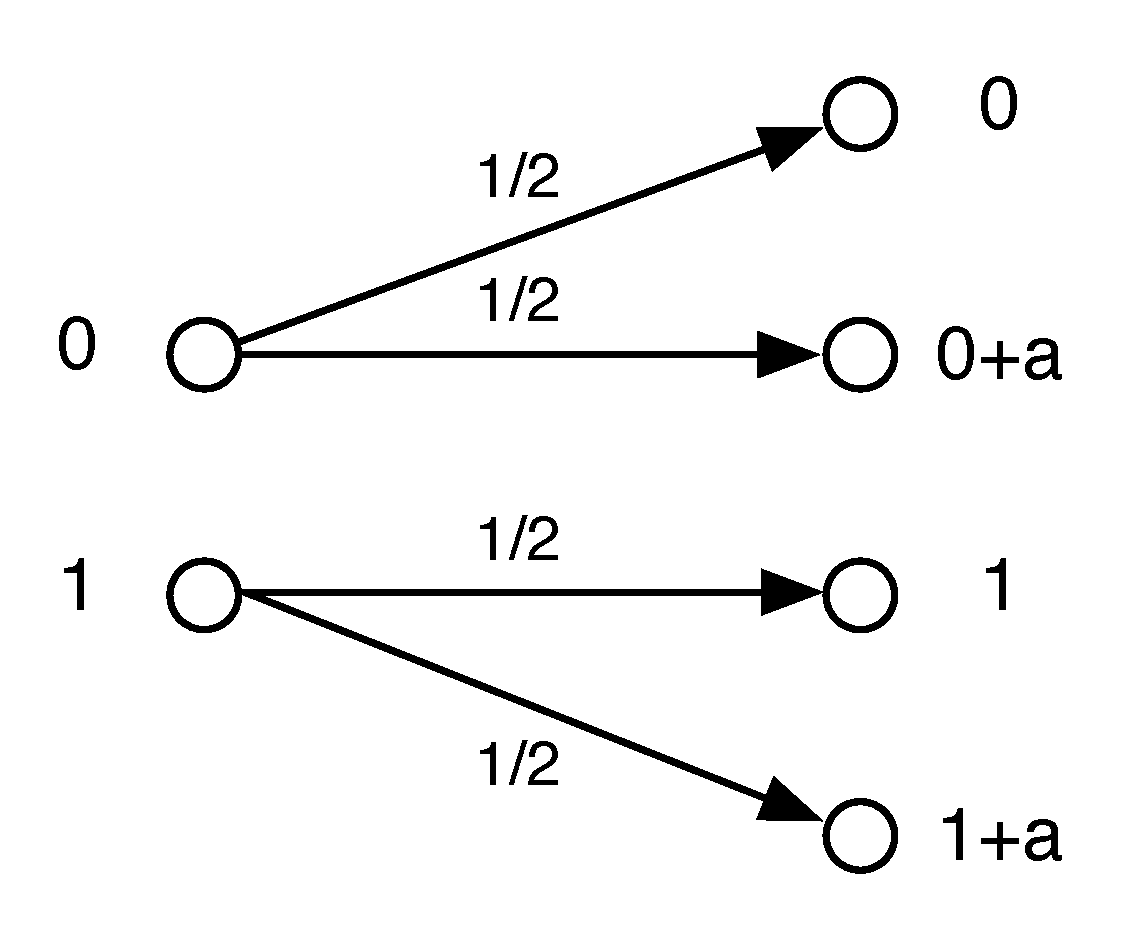
\includegraphics[width=0.4\textwidth]{img/gres.pdf}
       \caption{Grafo di canale}
       \label{fig:gres}
       \end{center}
       \end{figure}

       Poniamoci inizialmente nel caso in cui $a \neq 0$ e $a \neq 1$.
       Indicando con $\Pi$ $Pr\{X=0\}$, si ottiene:
       \[\begin{split}
        Pr\{Y=0\} &=\frac{\Pi}{2}  \\
        Pr\{Y=a\} &=\frac{\Pi}{2}  \\
        Pr\{Y=1\} &=\frac{1-\Pi}{2}  \\
        Pr\{Y=1+a\} &=\frac{1-\Pi}{2}  \\
        \end{split}
       \]
       Inoltre:
       \[
        H(Y/X=0)=H(Y/X=1)=H \left( \frac{1}{2},\frac{1}{2} \right)=1
       \]
       Quindi:
       \[\begin{split}
         I(X;Y) &=H(Y)-H(Y/X) \\
          &=H(Y)-\Pi H(Y/X=0) - (1-\Pi) H(Y/X=1) \\
          &=H(Y)-\Pi -1 + \Pi \\
          &=H(Y)-1 \\
          &=H \left (\frac{\Pi}{2},\frac{\Pi}{2},\frac{1-\Pi}{2},\frac{1-\Pi}{2} \right)-1 \\
         \end{split}
       \]
       Quindi la capacità è:
       \[
        C=\max_{p(x)} I(X;Y)
         =\max_{p(x)}H \left (\frac{\Pi}{2},\frac{\Pi}{2},\frac{1-\Pi}{2},\frac{1-\Pi}{2} \right)-1
       \]
       Ma il massimo dell'entropia si ha quando tutte le componenti sono uguali.
       In questo caso quindi si ha massimo quando valgono tutte 1/4, caso che si verifica per $\Pi=1/2$ (l'entropia 
       risulta invece log4=2).
       Risulta quindi:
       \[
        C=2-1=1 \ bit
       \]
       Restano da trattate i casi con a=0 e a=1. Se a=0, Y vale unicamente 0 o 1. Si ottiene un canale completamente 
       deterministico, la cui capacità è $C=log|X|=1$. Nel caso invece in cui a=1, Y assume i valori 0,1,2.
       In questo caso si ha un canale inutile, quindi la capacità è 0.
       Riassumendo:
       \[
        C=
        \begin{cases}
         1 & a \neq 1 \\
         0 & a =1 \\
         \end{cases}
        \]


       \bigskip
 \item Si calcoli la capacità del canale avente la seguente matrice di transizione:
      \[ P = \left(
        \begin{array}{ccccc}
           0.3  & 0.1  & 0.2 & 0.1 & 0.3 \\
           0.1  & 0.3  & 0.2 & 0.3 & 0.1\\
        \end{array} \right)
       \]
       e determinare una distribuzione di probabilità di ingresso in corrispondenza della quale si ottiene la capacità.
       \bigskip
       \bigskip

       \textit{Soluzione:}

       \noindent
       Si tratta di un canale debolmente simmetrico, pertanto:
       \[\begin{split}
        C &= log|Y|-H(r) \\
          &= log(5) - H(0.3,0.1,0.2,0.1,0.3) \\
          &\simeq 2.322 - 2.171 \\
          &\simeq 0.151 \ bit
         \end{split}
       \]
       La capacità si ottiene, sempre in virtù del fatto che il canale è debolmente simmetrico, quanto P(X) ha 
       distribuzione uniforme: X=(1/2,1/2).

       \bigskip
 \item In un canale binario, la probabilità che durante la trasmissione un bit venga complementato 
       (cioè, che da 0 diventi 1 e viceversa) è costante e pari a p=0.1.
        Assumendo che la sorgente che alimenta il canale invii un simbolo ogni secondo, è possibile 
        trasmettere informazione affidabile su questo canale ad una velocità superiore a 1 bit/sec. Perché?
       \bigskip
       \bigskip

       \textit{Soluzione:}

       \noindent
       Si tratta di un BSC, la cui capacità è:
       \[
        C=1-H(p)=1-H(0.1,0.9) \simeq 1-0.469 \simeq \ 0.531 bit
       \]
       Per il secondo teorema di Shannon, per trasmettere informazione affidabile deve essere :
       \[
        R \le C
       \]
       Ma in questo caso R=1 e quindi $R>C$. Pertanto non è possibile trasmettere sul canale ad 1 bit/sec in maniera 
       affidabile.
\end{enumerate}

\clearpage
\phantomsection 
\addcontentsline{toc}{chapter}{Bibliografia}

\begin{thebibliography}{3}

\bibitem{ct}
Gareth A. Jones, J. Mary Jones,
\newblock {\sl Information and Coding Theory},
\newblock Springer, London, 2000.

\bibitem{jj}
Thomas M. Cover, Joy A. Thomas,
\newblock {\sl Elements of  Information Theory},
\newblock Wiley, New York, 1991.


\bibitem{app}
Appunti delle lezioni raccolti da Stefano Calzavara, Anna Marabello, Lorenzo Simionato e Daniele Turato.

\end{thebibliography}


\end{document}